\documentclass[11pt,a4paper]{report}

% Language setting
\usepackage[english]{babel}

% Page layout
\usepackage[a4paper,top=2.5cm,bottom=2.5cm,left=3cm,right=3cm,marginparwidth=1.75cm]{geometry}

% Essential packages
\usepackage{amsmath,amsfonts,amssymb}
\usepackage{graphicx}
\usepackage{listings}
\usepackage{xcolor}
\usepackage{booktabs}
\usepackage{caption}
\usepackage{hyperref}
\usepackage{float}
\usepackage{natbib}

\usepackage{research-style}

% Set image paths for all section folders
\graphicspath{{assets/section1/}{assets/section2/}{assets/section3/}{assets/images}}

% Code listing configuration
\lstset{
    basicstyle=\footnotesize\ttfamily,
    breaklines=true,
    frame=single,
    language=Python,
    showstringspaces=false,
    commentstyle=\color{gray},
    keywordstyle=\color{blue},
    stringstyle=\color{red}
}

% Hyperref configuration
\hypersetup{
    colorlinks=true,
    linkcolor=blue,
    filecolor=magenta,
    urlcolor=cyan
}

\begin{document}

% Custom title page layout
\thispagestyle{empty}

% Logo at full width (stays at top)
\noindent

\includegraphics[width=\textwidth]{uchimi_logo.jpg}

% Use flexible space to center the remaining content
\vspace*{\fill}

% Center all content below logo
\begin{center}

% Summer Research School text - bigger
{\Large\textbf{Summer Research School 2025}}

\vspace{1.5em}

% Main title
{\Huge\textbf{Neural Network Engine}} \\[0.5em]
{\Large A Comprehensive Deep Learning Framework with Automatic Differentiation} \\[0.3em]
{\large and Research Software for Neural Network Education \& Experimentation}

\vspace{2.5em}

% Author section - larger with bold name and institution
{\large
\textbf{Author(s):} \\[1em]
\textbf{Matt Minev}\\
\textbf{PMPG "St. Kliment Ohridski", Montana, Bulgaria}\\
\texttt{matt.minev@gmail.com}
}

\vspace{2.5em}

% Scientific Advisor section - institution split to two lines
{\large
\textbf{Scientific Advisor(s):} \\[0.5em]
\textbf{Emil Kelevedjiev}\\
\textbf{Institute of Mathematics and Informatics,} \\
\textbf{Bulgarian Academy of Sciences}\\
\texttt{keleved@gmail.com}
}

\vspace{2.5em}

% Date at the bottom - bigger
{\large\today}

\end{center}

% Flexible space to balance the page
\vspace*{\fill}

\newpage

\begin{abstract}
The Neural Network Engine is a comprehensive machine learning framework built from first principles, implementing core deep learning concepts through practical, educational code. The engine features nine activation functions including ReLU, Sigmoid, Tanh, and advanced variants like Swish and GELU, paired with robust optimization algorithms including SGD with momentum and Adam optimizer.

The framework supports complete neural network workflows from data preprocessing through model training and evaluation. Three applications demonstrate its capabilities: a high-accuracy digit recognition system with interactive visualization, a universal character recognizer handling alphanumeric classification, and an innovative quadratic equation predictor exploring neural networks in mathematical problem-solving.

Key contributions include numerically stable implementations, automatic differentiation for gradient computation, modular architecture enabling rapid experimentation, and comprehensive performance monitoring tools. The engine successfully bridges theoretical understanding with practical implementation, making complex deep learning concepts accessible while providing robust tools for real-world pattern recognition and classification tasks.
\end{abstract}

\tableofcontents
\newpage

\chapter{Theoretical Foundations}

Neural networks form the cornerstone of modern artificial intelligence, representing sophisticated mathematical models capable of learning complex patterns from data. This chapter establishes the theoretical foundations underlying the Neural Network Engine, exploring both the fundamental principles of neural computation and the mathematical frameworks enabling efficient optimization. The theoretical understanding presented here provides the essential groundwork for comprehending the advanced implementation details and practical applications documented in subsequent chapters.

\section{Neural Networks Fundamentals}

\subsection{Historical Context and Biological Inspiration}

Neural networks draw inspiration from biological neural systems, where interconnected neurons process and transmit information through electrochemical signals. The mathematical formalization of these concepts began with McCulloch and Pitts in 1943, who demonstrated that networks of simple artificial neurons could perform logical operations. This foundational work established the theoretical basis for modern neural computation, proving that appropriately connected networks of binary threshold units could compute any logical function.

In artificial neural networks, this biological concept translates to computational models composed of interconnected processing units called \textbf{neurons} or \textbf{nodes}, each performing simple mathematical operations while collectively enabling complex pattern recognition and function approximation. The fundamental principle underlying neural networks is the concept of \textbf{distributed representation}, where information is encoded across multiple neurons rather than within individual units. This approach enables robust learning, generalization to unseen data, and fault tolerance—characteristics that make neural networks particularly effective for real-world applications.

The theoretical foundation for neural networks' computational power rests on several key mathematical principles. First, the \textbf{superposition principle} allows complex functions to be represented as weighted combinations of simpler functions. Second, the concept of \textbf{hierarchical feature learning} enables networks to automatically discover increasingly abstract representations through multiple layers of transformation. Third, the \textbf{non-linear composition} of simple operations creates systems capable of approximating arbitrarily complex mappings between input and output spaces.

\subsection{Network Architecture and Mathematical Structure}

A neural network consists of multiple \textbf{layers} of interconnected neurons, typically organized in a feedforward architecture. The mathematical structure of these networks can be precisely defined through a series of transformations operating on vector spaces.

\textbf{Input Layer}: Receives raw data features, with each neuron corresponding to a specific input dimension. For a dataset with $n$ features, the input layer contains $n$ neurons representing the feature vector $\mathbf{x} = [x_1, x_2, \ldots, x_n]^T \in \mathbb{R}^n$.

\textbf{Hidden Layers}: Intermediate layers that transform input data through learned representations. Each hidden layer $l$ contains $h_l$ neurons, where the number of layers $L$ and neurons per layer constitute the network's \textbf{architecture}. The architectural space can be formally defined as:
\begin{equation}
\mathcal{A} = \{(h_1, h_2, \ldots, h_L) : h_i \in \mathbb{N}^+, L \in \mathbb{N}^+\}
\end{equation}

\textbf{Output Layer}: Produces the final predictions, with the number of neurons determined by the specific task. For regression tasks with $m$ outputs, the output layer contains $m$ neurons producing $\hat{\mathbf{y}} \in \mathbb{R}^m$. For classification tasks with $C$ classes, the output typically consists of $C$ neurons representing class probabilities.

\textbf{Weights and Biases}: Each connection between neurons is associated with a \textbf{weight} $w_{ij}$ representing the strength of the connection from neuron $i$ to neuron $j$. The weight matrix for layer $l$ is denoted $\mathbf{W}^{(l)} \in \mathbb{R}^{h_l \times h_{l-1}}$, where $h_0 = n$ (input dimension). Additionally, each neuron has a \textbf{bias} term $b_j$ that shifts the activation function, collected in bias vector $\mathbf{b}^{(l)} \in \mathbb{R}^{h_l}$.

The total parameter space of a neural network is given by:
\begin{equation}
\Theta = \bigcup_{l=1}^{L} \{\mathbf{W}^{(l)}, \mathbf{b}^{(l)}\}
\end{equation}

with dimensionality:
\begin{equation}
|\Theta| = \sum_{l=1}^{L} (h_l \times h_{l-1} + h_l) = \sum_{l=1}^{L} h_l(h_{l-1} + 1)
\end{equation}

\begin{figure}[H]
\centering
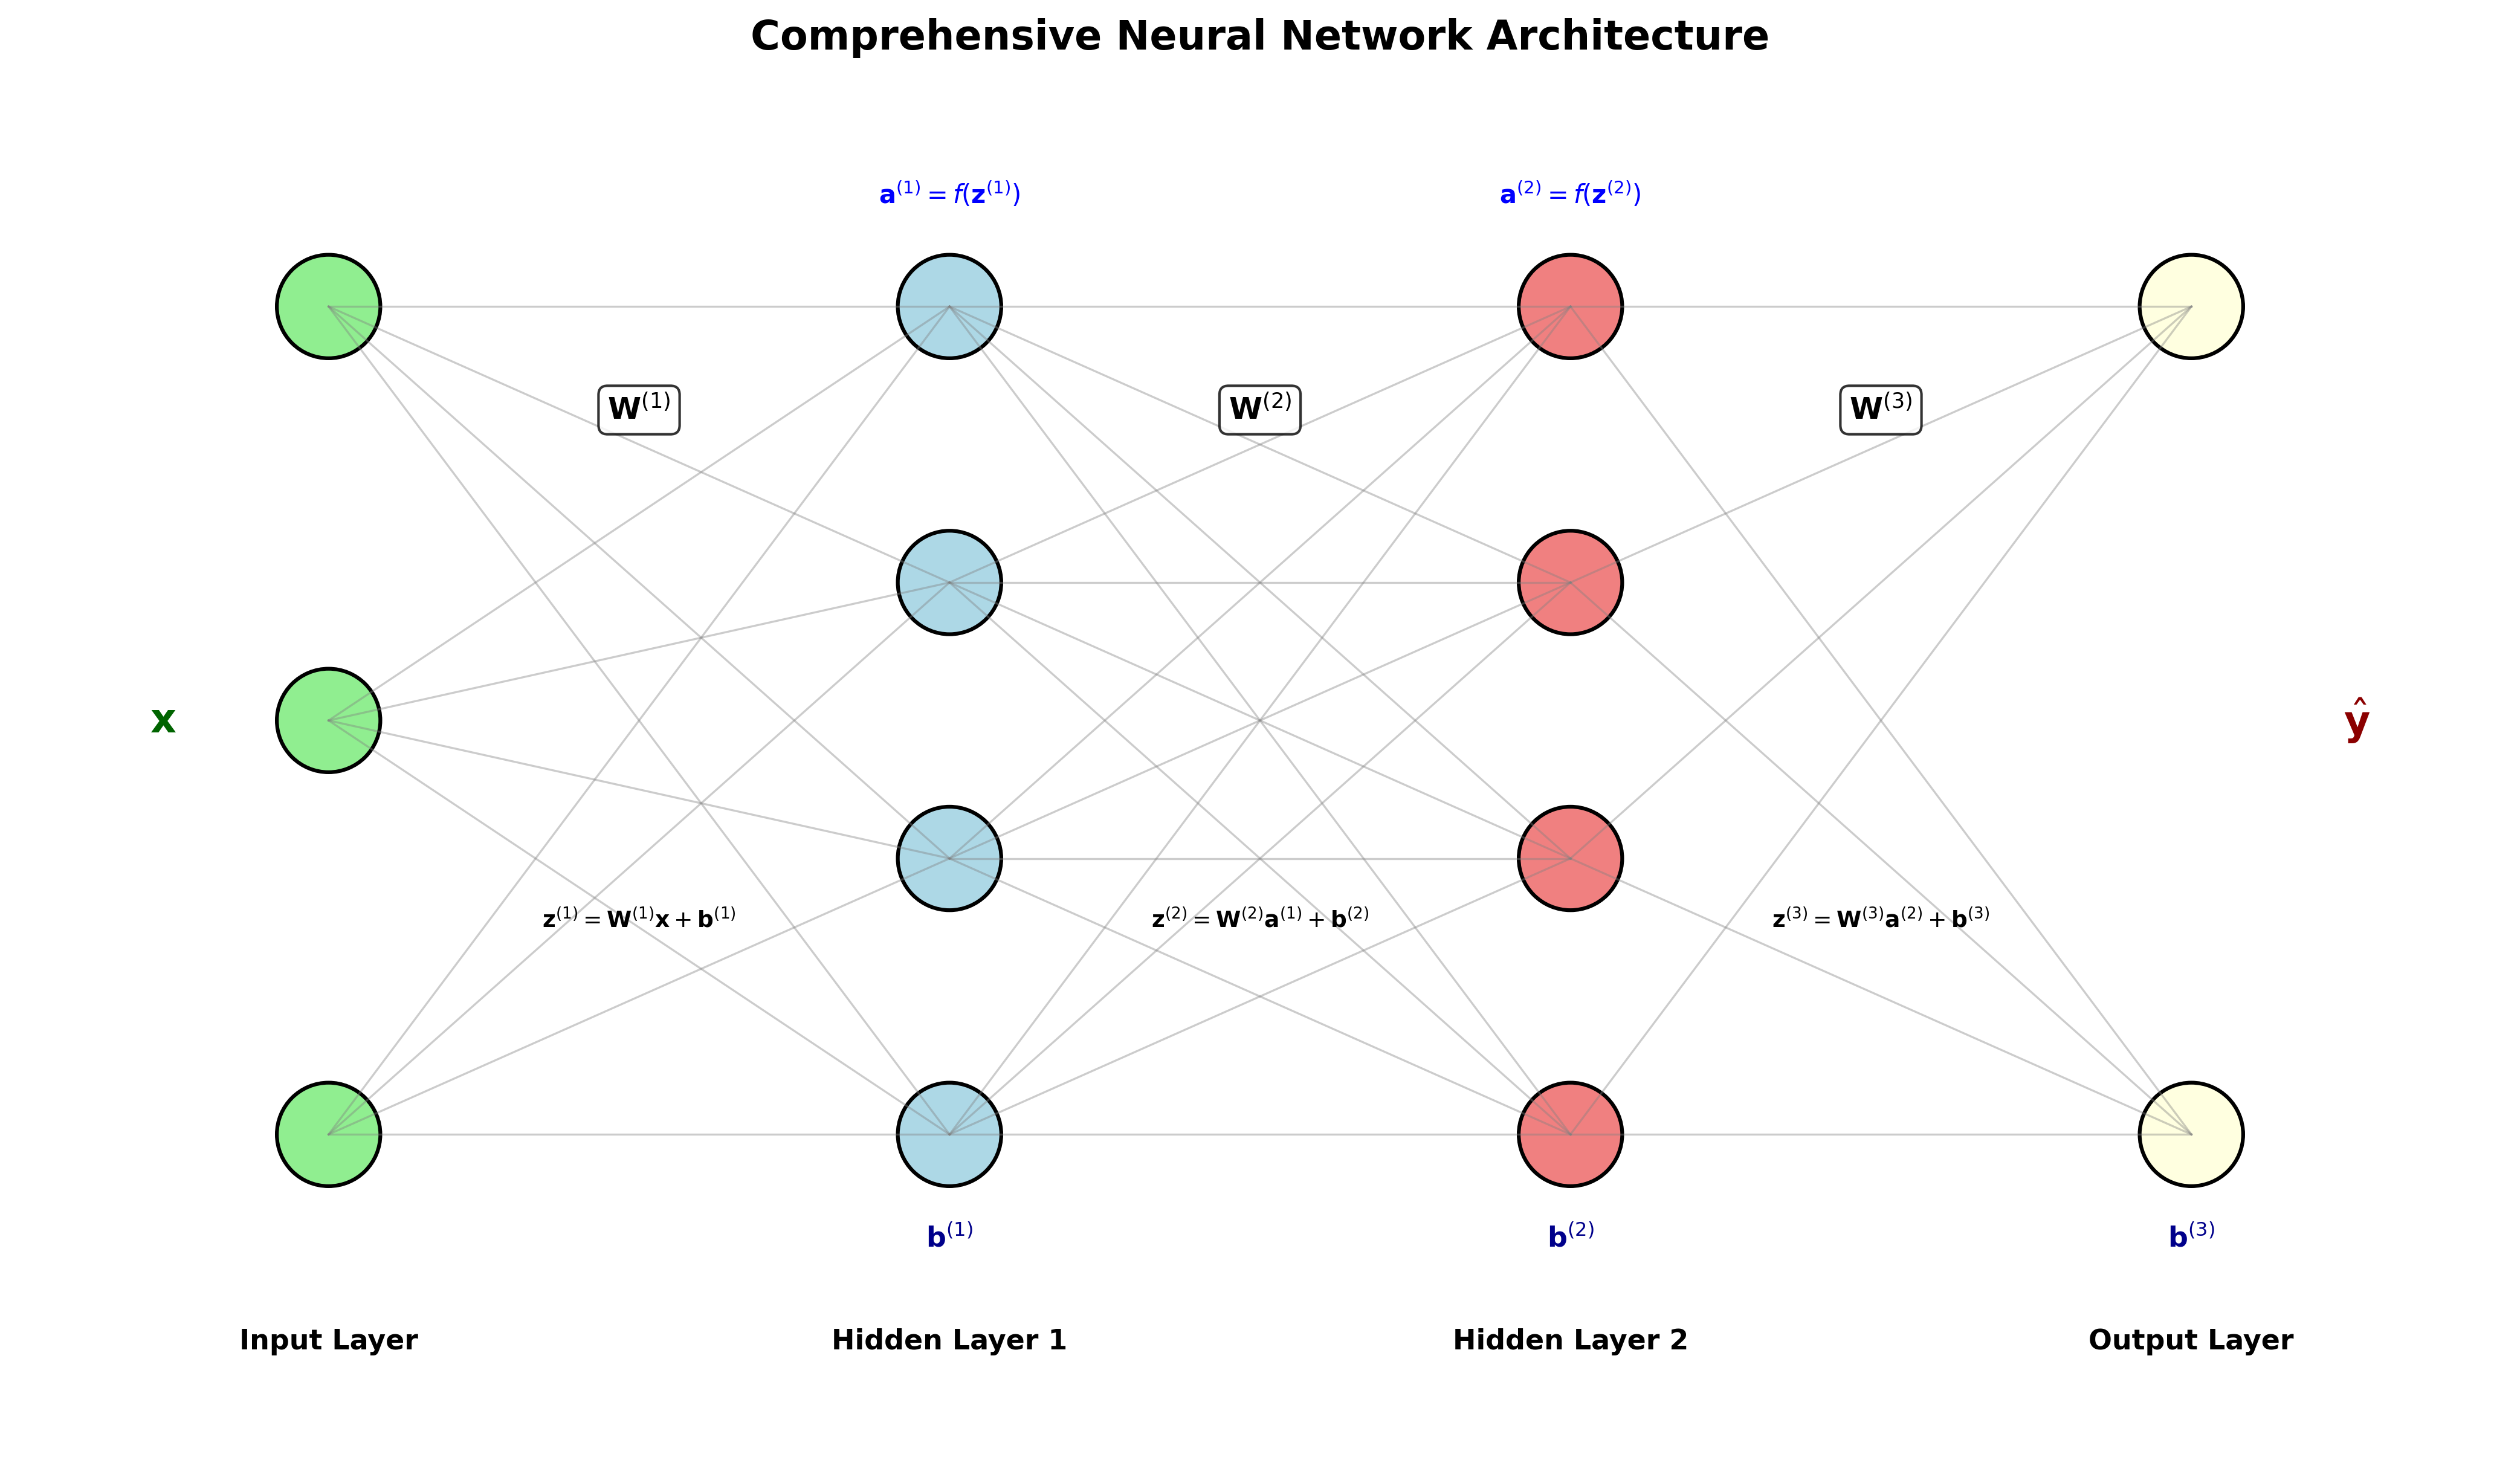
\includegraphics[width=1\textwidth]{neural_network_architecture.png}
\caption{Fundamental neural network architecture showing input layer, hidden layers, and output layer with interconnected neurons. Weights and biases control information flow between layers.}
\label{fig:nn_architecture}
\end{figure}

\subsection{Forward Propagation Mechanics and Mathematical Framework}

Forward propagation represents the process by which input data flows through the network to produce predictions. This process can be mathematically described as a composition of affine transformations followed by non-linear activations.

For a layer $l$ with input $\mathbf{a}^{(l-1)}$, the computation proceeds in two distinct stages:

\textbf{Linear Transformation}: The weighted sum of inputs plus bias terms:
\begin{equation}
\mathbf{z}^{(l)} = \mathbf{W}^{(l)} \mathbf{a}^{(l-1)} + \mathbf{b}^{(l)}
\end{equation}

where $\mathbf{W}^{(l)} \in \mathbb{R}^{h_l \times h_{l-1}}$ represents the weight matrix for layer $l$, and $\mathbf{b}^{(l)} \in \mathbb{R}^{h_l}$ denotes the bias vector.

\textbf{Nonlinear Activation}: Application of an activation function $f^{(l)}: \mathbb{R} \rightarrow \mathbb{R}$ to introduce nonlinearity:
\begin{equation}
\mathbf{a}^{(l)} = f^{(l)}(\mathbf{z}^{(l)})
\end{equation}

where the activation function is applied element-wise to the vector $\mathbf{z}^{(l)}$.

The complete forward pass can be expressed as a composition of functions:
\begin{equation}
\hat{\mathbf{y}} = f^{(L)}(\mathbf{W}^{(L)} f^{(L-1)}(\mathbf{W}^{(L-1)} \cdots f^{(1)}(\mathbf{W}^{(1)} \mathbf{x} + \mathbf{b}^{(1)}) \cdots + \mathbf{b}^{(L-1)}) + \mathbf{b}^{(L)})
\end{equation}

The activation function enables neural networks to approximate nonlinear relationships, as composition of linear transformations alone can only represent linear functions regardless of network depth. The mathematical necessity of nonlinearity can be proven: without activation functions, any deep network reduces to:
\begin{equation}
\mathbf{y} = \left(\prod_{l=1}^{L} \mathbf{W}^{(l)}\right) \mathbf{x} + \mathbf{b}_{combined}
\end{equation}

which is equivalent to a single-layer linear model.

\subsection{Universal Approximation Theory}

Neural networks function as \textbf{universal function approximators}, capable of approximating any continuous function to arbitrary precision given sufficient neurons and appropriate activation functions. This theoretical foundation, established by multiple formulations of the Universal Approximation Theorem, provides the mathematical justification for neural networks' effectiveness across diverse domains.

\textbf{Cybenko's Theorem (1989)}: Let $\sigma$ be a continuous, bounded, and non-constant activation function. Then finite linear combinations of the form:
\begin{equation}
G(x) = \sum_{j=1}^{N} \alpha_j \sigma(\mathbf{w}_j^T \mathbf{x} + b_j)
\end{equation}
are dense in $C(I_n)$, the space of continuous functions on the unit hypercube $I_n = [0,1]^n$, with respect to the uniform norm.

\textbf{Hornik's Generalization (1991)}: The universal approximation property holds for any bounded, non-constant activation function that is not a polynomial. This significantly broadens the class of admissible activation functions.

\textbf{Modern Formulations}: Recent work has extended these results to provide explicit bounds on approximation errors and required network width. For a function $f: [0,1]^n \rightarrow \mathbb{R}$ with bounded variation, there exists a neural network with one hidden layer containing at most $\mathcal{O}(\epsilon^{-n})$ neurons that approximates $f$ within error $\epsilon$.

The practical implications of these theorems are profound:
- \textbf{Existence Guarantee}: For any continuous function on a compact domain, there exists a neural network that can approximate it arbitrarily well.
- \textbf{Architecture Independence}: The approximation property depends primarily on width rather than depth for universal approximation.
- \textbf{Activation Function Requirements}: The activation function must be non-polynomial and non-constant for universal approximation to hold.

However, these theorems do not address:
- \textbf{Constructibility}: How to find the optimal weights and biases
- \textbf{Efficiency}: The number of parameters required may be exponential in the input dimension
- \textbf{Learnability}: Whether gradient-based methods can find good approximations

\subsection{Loss Functions and Learning Objectives}

The learning process involves optimizing a \textbf{loss function} $L(\mathbf{y}, \hat{\mathbf{y}})$ that measures the discrepancy between predicted outputs $\hat{\mathbf{y}}$ and true targets $\mathbf{y}$. The choice of loss function fundamentally shapes the learning dynamics and determines what aspects of the data the model emphasizes during training.

\textbf{Mean Squared Error (MSE)} for regression tasks:
\begin{equation}
L_{MSE} = \frac{1}{n} \sum_{i=1}^{n} \|\mathbf{y}_i - \hat{\mathbf{y}}_i\|^2
\end{equation}

The MSE loss assumes Gaussian noise in the data and corresponds to maximum likelihood estimation under this assumption. Its quadratic nature provides strong gradients far from the optimum but can be sensitive to outliers.

\textbf{Cross-Entropy Loss} for classification tasks:
\begin{equation}
L_{CE} = -\frac{1}{n} \sum_{i=1}^{n} \sum_{c=1}^{C} y_{i,c} \log(\hat{y}_{i,c})
\end{equation}

where $C$ represents the number of classes, $y_{i,c}$ is the true label (one-hot encoded), and $\hat{y}_{i,c}$ is the predicted probability for class $c$.

Cross-entropy loss emerges naturally from the maximum likelihood principle when assuming categorical distributions. Its logarithmic nature provides strong gradients when predictions are incorrect and approaches zero when predictions are confident and correct.

\textbf{Regularized Loss Functions}: To prevent overfitting, regularization terms are often added to the base loss:
\begin{equation}
L_{total} = L_{data}(\mathbf{y}, \hat{\mathbf{y}}) + \lambda R(\Theta)
\end{equation}

where $R(\Theta)$ is a regularization term and $\lambda$ controls the regularization strength. Common regularization forms include:
- \textbf{L1 Regularization}: $R(\Theta) = \sum_{i} |\theta_i|$ promotes sparsity
- \textbf{L2 Regularization}: $R(\Theta) = \sum_{i} \theta_i^2$ penalizes large weights
- \textbf{Elastic Net}: $R(\Theta) = \alpha \sum_{i} |\theta_i| + (1-\alpha) \sum_{i} \theta_i^2$ combines L1 and L2

\subsection{Activation Functions and Their Mathematical Properties}

Activation functions serve as the nonlinear elements that enable neural networks to learn complex patterns. Each activation function has distinct mathematical properties that affect network behavior, training dynamics, and representational capacity.

\textbf{Sigmoid Function}:
\begin{equation}
\sigma(z) = \frac{1}{1 + e^{-z}}, \quad \sigma'(z) = \sigma(z)(1 - \sigma(z))
\end{equation}

The sigmoid function maps inputs to $(0, 1)$ and has a smooth, S-shaped curve. However, its derivative is bounded by $[0, 0.25]$, leading to vanishing gradient problems in deep networks.

\textbf{Hyperbolic Tangent}:
\begin{equation}
\tanh(z) = \frac{e^z - e^{-z}}{e^z + e^{-z}}, \quad \tanh'(z) = 1 - \tanh^2(z)
\end{equation}

Tanh maps inputs to $(-1, 1)$ and is zero-centered, which can improve convergence properties. Like sigmoid, it suffers from vanishing gradients due to its bounded derivative $[0, 1]$.

\textbf{Rectified Linear Unit (ReLU)}:
\begin{equation}
\text{ReLU}(z) = \max(0, z), \quad \text{ReLU}'(z) = \begin{cases} 1 & \text{if } z > 0 \\ 0 & \text{if } z \leq 0 \end{cases}
\end{equation}

ReLU addresses the vanishing gradient problem by providing a constant gradient of 1 for positive inputs. However, it can suffer from "dying ReLU" problem, where neurons become permanently inactive.

Advanced activation functions implemented in Neural Engine are detailed in Section 2.2, where we explore the mathematical properties and implementation considerations of various activation functions including ELU, Swish, and GELU variants.

\subsection{Applications in Modern AI and Computational Complexity}

Neural networks have revolutionized numerous domains through their ability to learn complex patterns from data. The theoretical foundations established above enable practical applications across diverse fields:

\textbf{Computer Vision}: Convolutional neural networks leverage translation equivariance and local connectivity to achieve superhuman performance in image recognition, object detection, and medical image analysis. The theoretical basis lies in the approximation of locally-varying functions through spatially-structured weight sharing.

\textbf{Natural Language Processing}: Transformer architectures have transformed language understanding through self-attention mechanisms that enable parallel computation of sequential dependencies. The mathematical foundation involves multi-head attention as learned similarity metrics in high-dimensional spaces.

\textbf{Scientific Computing}: Neural networks increasingly solve complex scientific problems, from protein folding prediction to climate modeling and quantum chemistry. Physics-informed neural networks (PINNs) incorporate differential equations directly into the loss function, enabling principled solutions to partial differential equations.

\textbf{Control Systems}: Deep reinforcement learning enables autonomous systems in robotics, game playing, and resource optimization through the marriage of neural function approximation with dynamic programming principles.

The computational complexity of neural network training scales as $\mathcal{O}(|\Theta| \cdot n \cdot T)$ where $|\Theta|$ is the number of parameters, $n$ is the number of training examples, and $T$ is the number of training iterations. Modern hardware accelerators (GPUs, TPUs) exploit the inherent parallelism in matrix operations to achieve practical training times for networks with millions or billions of parameters.

\section{Automatic Differentiation Theory}

\subsection{Mathematical Foundations and Historical Development}

Automatic differentiation forms the computational backbone of neural network training, enabling efficient calculation of gradients necessary for optimization algorithms. Unlike numerical differentiation, which suffers from approximation errors and requires $\mathcal{O}(n)$ function evaluations for $n$ variables, automatic differentiation provides exact gradients with computational complexity proportional to the original function evaluation.

The fundamental principle relies on the mathematical fact that any computer program can be decomposed into a sequence of elementary mathematical operations (addition, multiplication, exponential, logarithm, etc.), each with known derivatives. By systematically applying the chain rule to these elementary operations, automatic differentiation computes exact derivatives efficiently.

Automatic differentiation exploits the structure of computational graphs to achieve this efficiency. Every function computed by a program can be represented as a directed acyclic graph where:
- \textbf{Vertices} represent variables (inputs, intermediates, outputs)  
- \textbf{Edges} represent elementary operations
- \textbf{Forward evaluation} computes function values
- \textbf{Reverse evaluation} computes derivatives

The theoretical foundation rests on the chain rule of multivariable calculus. For a composite function $f(\mathbf{x}) = f_n(f_{n-1}(\cdots f_1(\mathbf{x}) \cdots))$, the Jacobian matrix is:
\begin{equation}
\frac{\partial \mathbf{f}}{\partial \mathbf{x}} = \frac{\partial f_n}{\partial f_{n-1}} \frac{\partial f_{n-1}}{\partial f_{n-2}} \cdots \frac{\partial f_1}{\partial \mathbf{x}}
\end{equation}

\subsection{Forward Mode vs. Reverse Mode Automatic Differentiation}

Two distinct modes of automatic differentiation exist, each with different computational characteristics and optimal use cases.

\textbf{Forward Mode Automatic Differentiation} computes directional derivatives by propagating derivative information forward through the computational graph. For a function $f: \mathbb{R}^n \rightarrow \mathbb{R}^m$, forward mode computes the Jacobian-vector product $\mathbf{J}\mathbf{v}$ where $\mathbf{v} \in \mathbb{R}^n$ is a direction vector.

The computational complexity is $\mathcal{O}(n \cdot \text{cost}(f))$ to compute all partial derivatives, making forward mode efficient when $n \ll m$ (few inputs, many outputs). This occurs in scenarios like sensitivity analysis or parameter optimization with few parameters.

\textbf{Reverse Mode Automatic Differentiation} (backpropagation) computes gradients by propagating derivative information backward through the computational graph. For the same function, reverse mode computes the vector-Jacobian product $\mathbf{v}^T\mathbf{J}$ where $\mathbf{v} \in \mathbb{R}^m$.

The computational complexity is $\mathcal{O}(m \cdot \text{cost}(f))$ to compute all partial derivatives, making reverse mode efficient when $m \ll n$ (many inputs, few outputs). This is precisely the case for neural networks, where there are typically millions of parameters but a single scalar loss function.

The mathematical relationship between forward and reverse mode can be understood through the duality of differentiation and integration. Forward mode corresponds to computing $\int \nabla f(\mathbf{x}) \cdot \mathbf{v} \, d\mathbf{v}$ while reverse mode computes $\int \mathbf{u}^T \nabla f(\mathbf{x}) \, d\mathbf{u}$.

\subsection{The Chain Rule and Computational Graph Theory}

The chain rule provides the mathematical foundation for backpropagation, enabling gradient computation through composite functions. For a composite function $f(g(\mathbf{x}))$, the derivative with respect to $\mathbf{x}$ is:

\begin{equation}
\frac{\partial f}{\partial \mathbf{x}} = \frac{\partial f}{\partial g} \cdot \frac{\partial g}{\partial \mathbf{x}}
\end{equation}

In neural networks, this extends to multiple variables and layers. For a loss function $L$ with respect to parameters $\theta^{(l)}$ in layer $l$:

\begin{equation}
\frac{\partial L}{\partial \theta^{(l)}} = \frac{\partial L}{\partial \mathbf{a}^{(L)}} \cdot \frac{\partial \mathbf{a}^{(L)}}{\partial \mathbf{a}^{(L-1)}} \cdots \frac{\partial \mathbf{a}^{(l+1)}}{\partial \mathbf{a}^{(l)}} \cdot \frac{\partial \mathbf{a}^{(l)}}{\partial \theta^{(l)}}
\end{equation}

where $L$ denotes the output layer and the chain of partial derivatives represents the gradient flow through the network.

The computational graph representation enables systematic application of the chain rule. Each node in the graph corresponds to an elementary operation with known local derivatives. The global derivative is computed by traversing the graph and applying the chain rule at each node.

\textbf{Graph Topology Considerations}: The structure of the computational graph affects both memory requirements and computational efficiency. Linear graphs (sequential operations) require minimal memory but may be computationally inefficient. Tree-like structures enable parallel computation but require careful memory management. Cycles in the graph (as in recurrent networks) require special handling through techniques like backpropagation through time.

\begin{figure}[H]
\centering
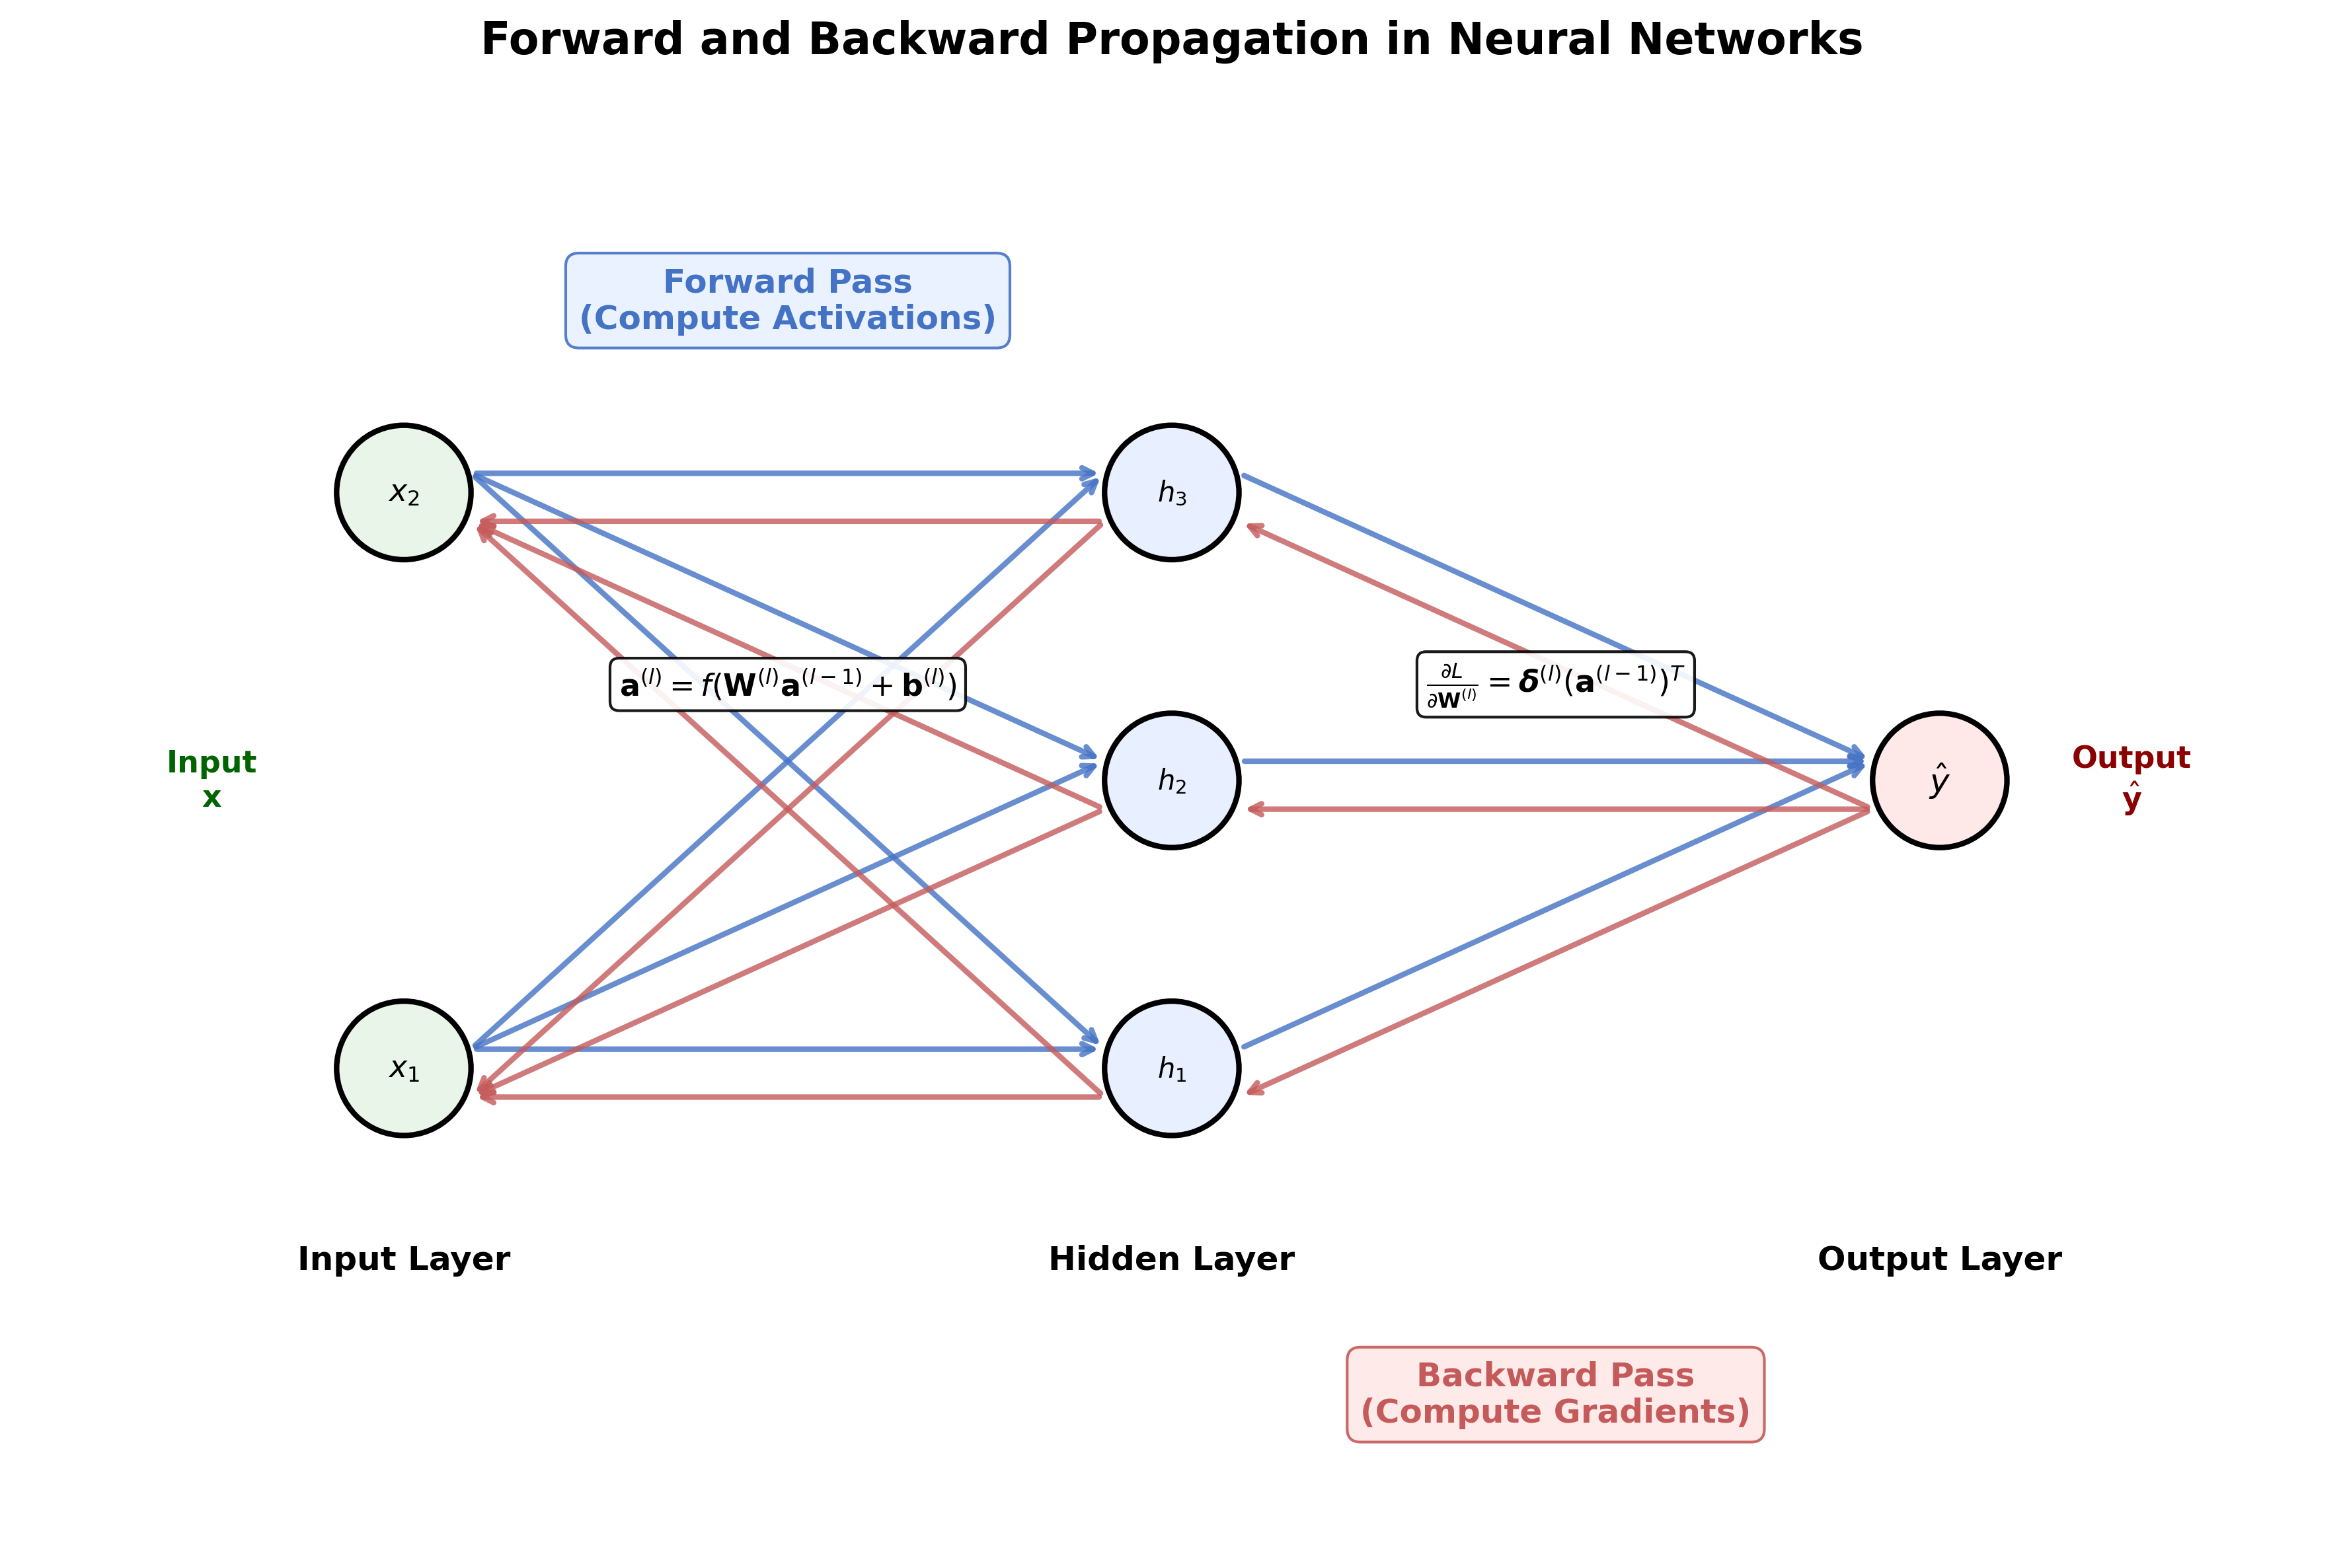
\includegraphics[width=0.9\textwidth]{gradient_flow_diagram.png}
\caption{Gradient flow illustration showing backpropagation through a neural network. Forward pass (blue arrows) computes activations, while backward pass (red arrows) propagates gradients for parameter updates.}
\label{fig:gradient_flow}
\end{figure}

\subsection{Backpropagation Algorithm: Mathematical Derivation and Implementation}

Backpropagation represents the practical implementation of automatic differentiation for neural networks, computing gradients by traversing the network in reverse order. The algorithm proceeds in two phases with rigorous mathematical foundations.

\textbf{Forward Pass}: Compute activations for all layers:
\begin{align}
\mathbf{z}^{(l)} &= \mathbf{W}^{(l)} \mathbf{a}^{(l-1)} + \mathbf{b}^{(l)} \\
\mathbf{a}^{(l)} &= f^{(l)}(\mathbf{z}^{(l)})
\end{align}

where $\mathbf{a}^{(0)} = \mathbf{x}$ (input) and $f^{(l)}$ is the activation function for layer $l$.

\textbf{Backward Pass}: Compute gradients starting from the output layer using the chain rule:

For the output layer $L$:
\begin{equation}
\boldsymbol{\delta}^{(L)} = \frac{\partial L}{\partial \mathbf{z}^{(L)}} = \frac{\partial L}{\partial \mathbf{a}^{(L)}} \odot f'^{(L)}(\mathbf{z}^{(L)})
\end{equation}

For hidden layers $l = L-1, L-2, \ldots, 1$:
\begin{equation}
\boldsymbol{\delta}^{(l)} = (\mathbf{W}^{(l+1)})^T \boldsymbol{\delta}^{(l+1)} \odot f'^{(l)}(\mathbf{z}^{(l)})
\end{equation}

where $\odot$ denotes element-wise multiplication and $\boldsymbol{\delta}^{(l)}$ represents the error gradient for layer $l$.

Finally, parameter gradients are computed as:
\begin{align}
\frac{\partial L}{\partial \mathbf{W}^{(l)}} &= \boldsymbol{\delta}^{(l)} (\mathbf{a}^{(l-1)})^T \\
\frac{\partial L}{\partial \mathbf{b}^{(l)}} &= \boldsymbol{\delta}^{(l)}
\end{align}

\textbf{Mathematical Correctness}: The correctness of backpropagation follows from the chain rule applied to the composite function representing the neural network. Each $\boldsymbol{\delta}^{(l)}$ represents the partial derivative of the loss with respect to the pre-activation $\mathbf{z}^{(l)}$, and the recursive relationship ensures proper accumulation of gradients through the network.

\textbf{Computational Complexity}: The time complexity of backpropagation is $\mathcal{O}(E)$ where $E$ is the number of edges (connections) in the network. This is optimal since each parameter must be updated at least once. The space complexity is $\mathcal{O}(V)$ where $V$ is the number of neurons, as activations must be stored for the backward pass.

\subsection{Optimization Landscapes and Mathematical Challenges}

Neural network optimization presents unique mathematical challenges due to the high-dimensional, non-convex nature of the loss landscape. Understanding these challenges is crucial for developing effective training strategies.

\textbf{Local Minima}: The loss function may contain numerous local minima, potentially trapping optimization algorithms away from the global optimum. However, recent theoretical work suggests that in sufficiently wide networks, most local minima are nearly as good as the global minimum due to the loss landscape's structure.

\textbf{Saddle Points}: High-dimensional spaces contain exponentially more saddle points than local minima, where gradients vanish but the point is not optimal. The prevalence of saddle points follows from random matrix theory: in an $n$-dimensional space, the probability that all eigenvalues of the Hessian are positive (indicating a local minimum) decreases exponentially with $n$.

\textbf{Vanishing Gradients}: In deep networks, gradients may become exponentially small in early layers, hindering learning of lower-level features. This occurs when the product of derivatives through many layers becomes very small:
\begin{equation}
\frac{\partial L}{\partial \mathbf{W}^{(1)}} = \frac{\partial L}{\partial \mathbf{a}^{(L)}} \prod_{l=L}^{2} \frac{\partial \mathbf{a}^{(l)}}{\partial \mathbf{a}^{(l-1)}} \frac{\partial \mathbf{a}^{(1)}}{\partial \mathbf{W}^{(1)}}
\end{equation}

If each factor $\|\frac{\partial \mathbf{a}^{(l)}}{\partial \mathbf{a}^{(l-1)}}\| < 1$, the gradient magnitude decays exponentially with depth.

\textbf{Exploding Gradients}: Conversely, gradients may grow exponentially, causing unstable training dynamics. This occurs when $\|\frac{\partial \mathbf{a}^{(l)}}{\partial \mathbf{a}^{(l-1)}}\| > 1$ for multiple layers, leading to exponential growth in gradient magnitudes.

Mathematical analysis reveals that the gradient magnitude is governed by the spectral properties of the weight matrices. For a network with identical layers, the gradient scaling is approximately:
\begin{equation}
\|\frac{\partial L}{\partial \mathbf{W}^{(1)}}\| \approx \|\frac{\partial L}{\partial \mathbf{a}^{(L)}}\| \prod_{l=1}^{L-1} \sigma_{\max}(\mathbf{W}^{(l)}) \prod_{l=1}^{L-1} \left(f'_{\max}\right)^{(l)}
\end{equation}

where $\sigma_{\max}$ is the maximum singular value and $f'_{\max}$ is the maximum derivative of the activation function.

\begin{figure}[H]
\centering
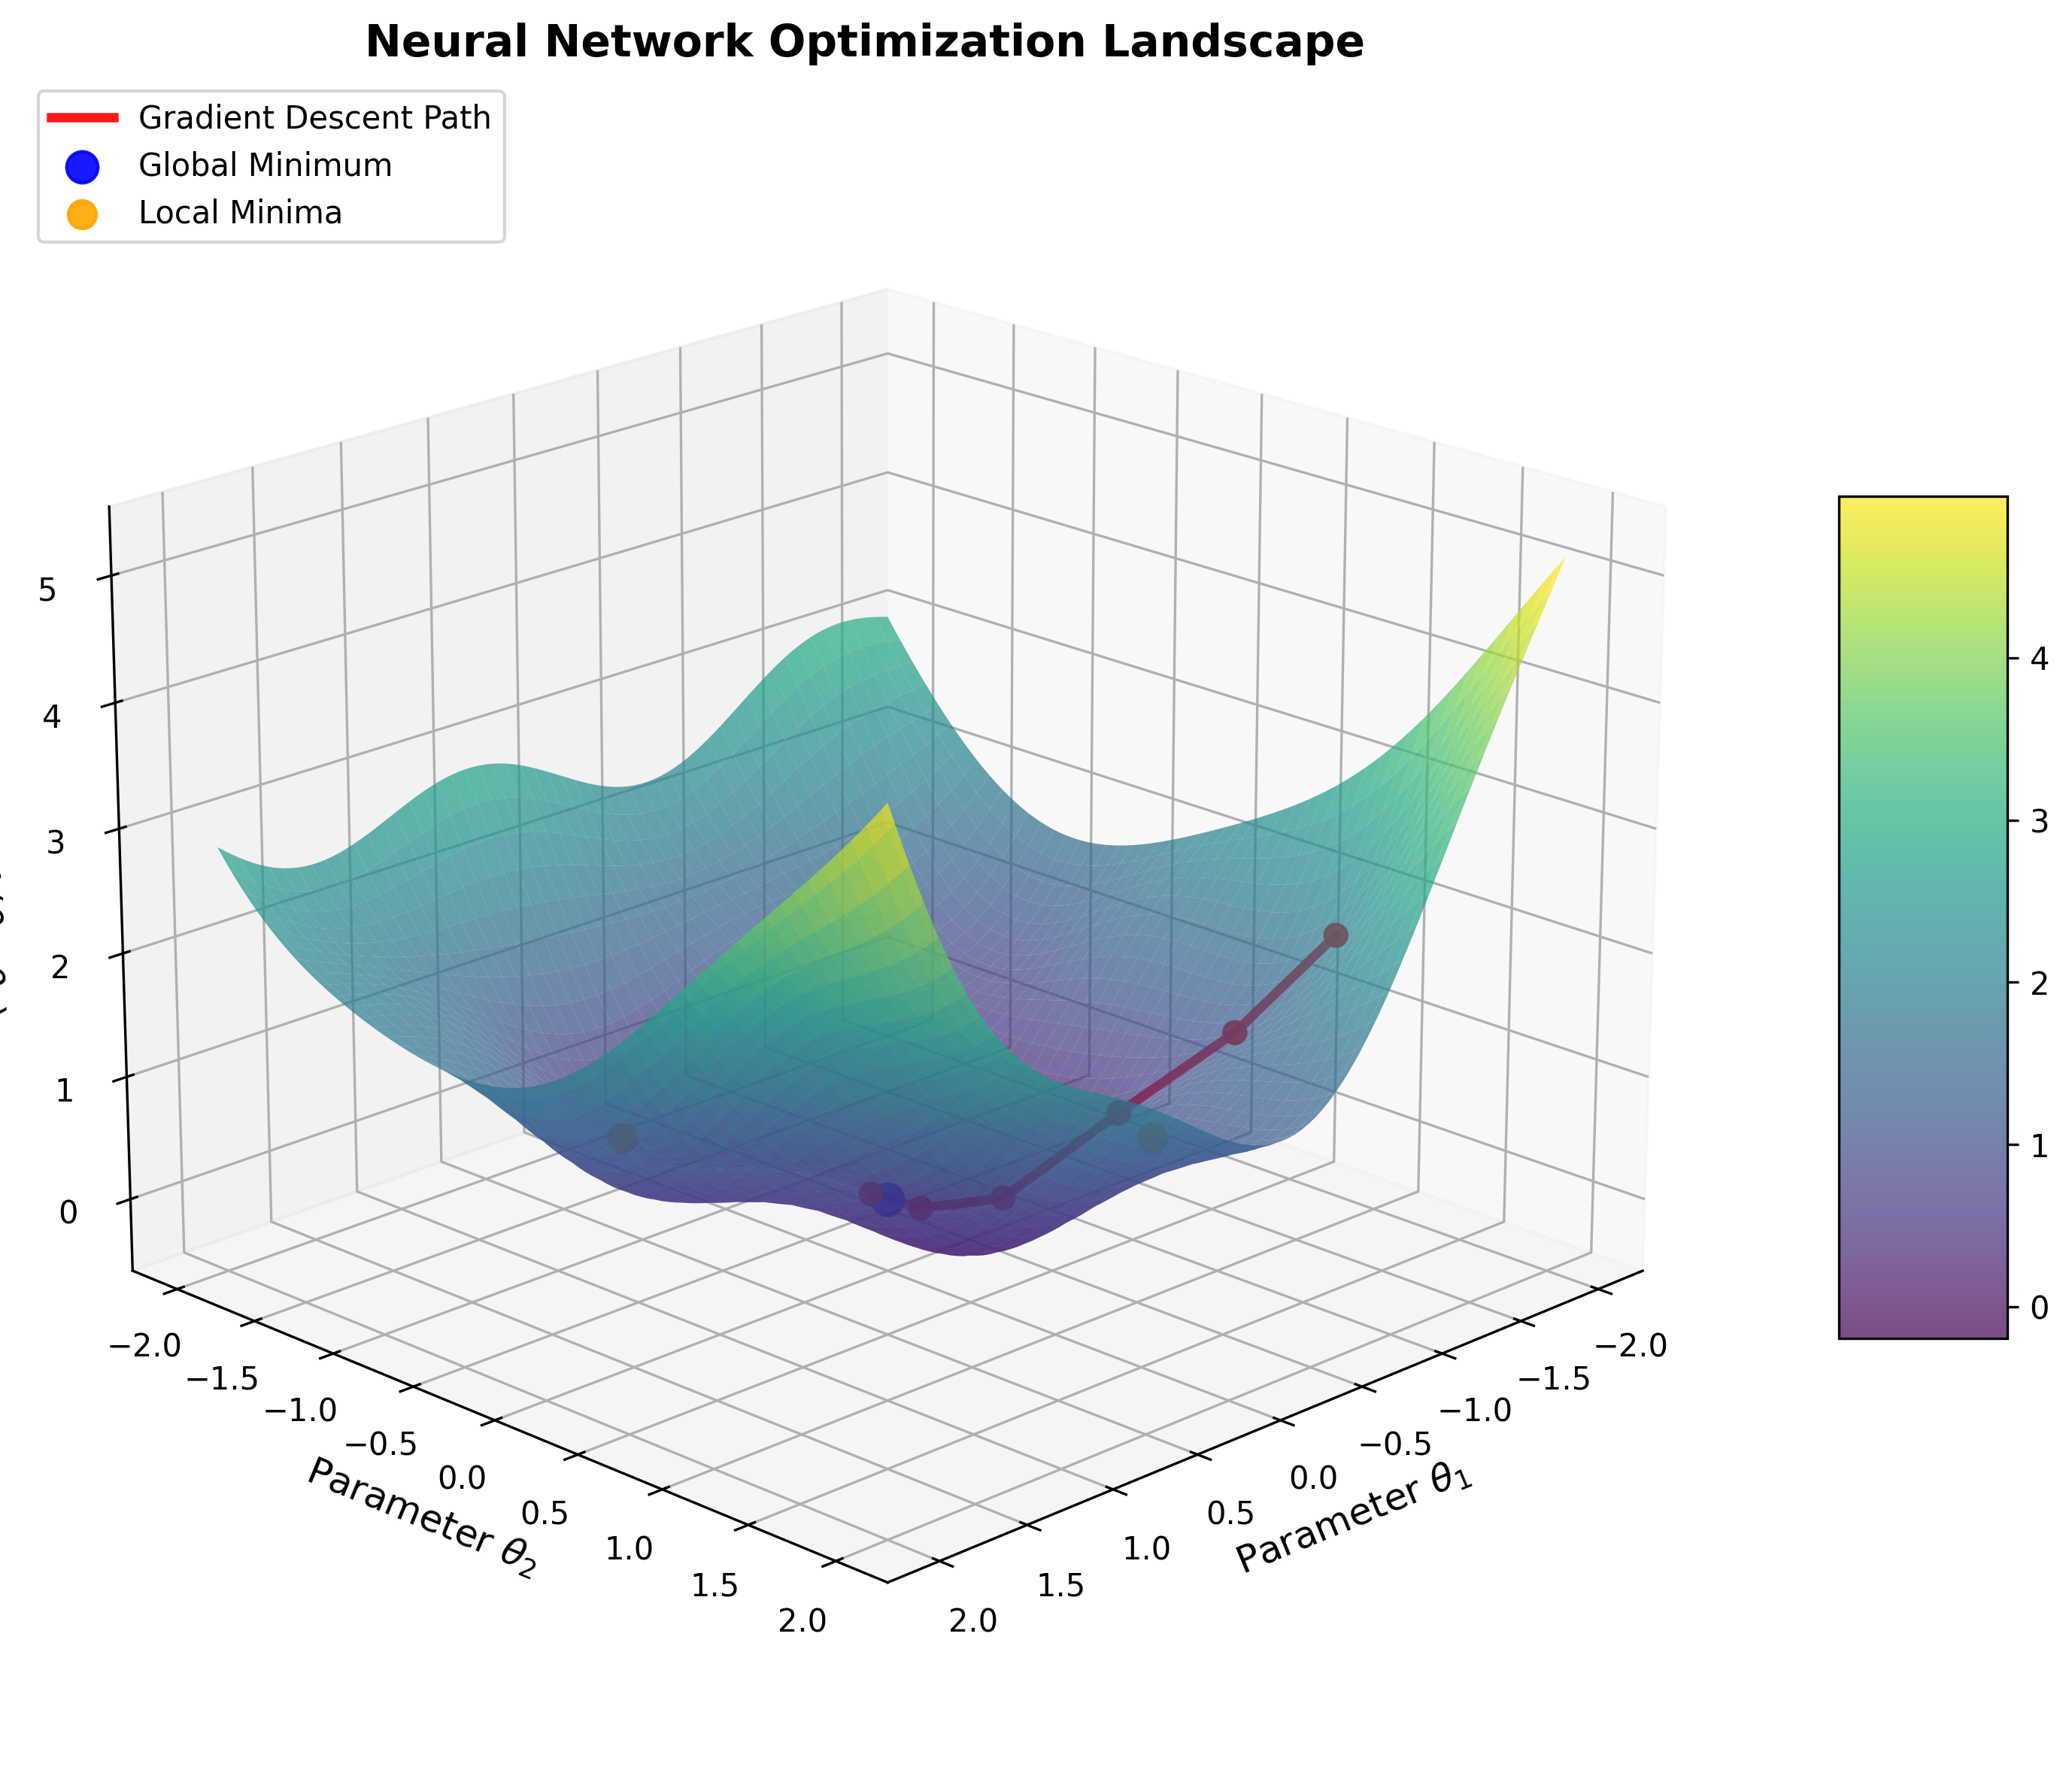
\includegraphics[width=0.8\textwidth]{optimization_landscape.png}
\caption{Visualization of neural network optimization landscape showing local minima, saddle points, and gradient descent trajectories. The complex topology illustrates challenges in finding global optima.}
\label{fig:optimization_landscape}
\end{figure}

\subsection{Advanced Topics in Automatic Differentiation}

Modern implementations of automatic differentiation incorporate several advanced techniques to address computational and numerical challenges.

\textbf{Checkpointing and Memory Optimization}: Training large networks requires careful memory management during backpropagation. Gradient checkpointing trades computation for memory by recomputing certain forward pass values during the backward pass rather than storing them. The optimal checkpointing strategy minimizes total computational cost subject to memory constraints.

\textbf{Higher-Order Derivatives}: Some applications require second-order derivatives (Hessians) for optimization methods like Newton's method or uncertainty quantification. Forward-over-reverse automatic differentiation can compute Hessian-vector products efficiently:
\begin{equation}
\mathbf{H}\mathbf{v} = \nabla_{\mathbf{x}} [(\nabla_{\mathbf{x}} f(\mathbf{x}))^T \mathbf{v}]
\end{equation}

This requires two passes: a forward pass to compute $\nabla f(\mathbf{x})$, then automatic differentiation of the directional derivative $(\nabla f(\mathbf{x}))^T \mathbf{v}$.

\textbf{Numerical Stability}: Automatic differentiation can suffer from numerical instability when function values become very large or small. Techniques like logarithmic transformations, numerically stable implementations of specific functions (e.g., softmax), and careful ordering of operations help maintain numerical precision.

\subsection{Computational Efficiency and Implementation Considerations}

Efficient automatic differentiation requires careful consideration of computational and memory complexity, particularly in modern deep learning frameworks.

\textbf{Forward vs. Reverse Mode Selection}: The choice between forward and reverse mode depends on the computational graph structure:
- Forward mode: optimal when $n_{\text{inputs}} \ll n_{\text{outputs}}$
- Reverse mode: optimal when $n_{\text{outputs}} \ll n_{\text{inputs}}$  
- Mixed mode: combinations can be optimal for complex graphs

The crossover point typically occurs when the number of inputs approximately equals the number of outputs.

\textbf{Memory Management Strategies}: Backpropagation requires storing intermediate activations for gradient computation, leading to memory complexity proportional to network depth. Advanced strategies include:
- \textbf{Activation Checkpointing}: Store only subset of activations, recompute others
- \textbf{Gradient Accumulation}: Aggregate gradients over multiple micro-batches
- \textbf{Memory-Efficient Implementations}: Exploit specific architectural patterns (e.g., reversible layers)

\textbf{Computational Graph Optimization}: Modern frameworks perform graph-level optimizations:
- \textbf{Operation Fusion}: Combine multiple operations into single kernels
- \textbf{Memory Pooling}: Reuse memory buffers across operations  
- \textbf{Parallel Execution}: Execute independent operations simultaneously
- \textbf{Just-in-Time Compilation}: Optimize execution for specific hardware

The theoretical complexity of reverse-mode automatic differentiation is $\mathcal{O}(E)$ where $E$ represents the number of edges in the computational graph. This makes it remarkably efficient compared to naive gradient computation methods that would require $\mathcal{O}(nE)$ operations for $n$ parameters. In practice, optimized implementations achieve constant factors close to this theoretical minimum.

\textbf{Parallelization Strategies}: Modern hardware (GPUs, TPUs) enables massive parallelization of automatic differentiation:
- \textbf{Data Parallelism}: Process multiple samples simultaneously
- \textbf{Model Parallelism}: Distribute network layers across devices
- \textbf{Pipeline Parallelism}: Overlap forward and backward passes
- \textbf{SIMD Operations}: Vectorize element-wise operations

These parallelization strategies can achieve near-linear speedups for appropriately designed networks and datasets, making training of large-scale models computationally feasible.

Specific optimizers implemented in Neural Engine are covered in Section 2.3, where we explore advanced optimization algorithms that address the challenges outlined in this theoretical foundation, including adaptive learning rates, momentum methods, and second-order approximations.


\chapter{Neural Engine Architecture}

This chapter provides an exhaustive technical analysis of the Neural Network Engine implementation, examining every component from fundamental design philosophy through detailed mathematical formulations. The engine represents a sophisticated yet educational framework that demonstrates modern deep learning principles through transparent, from-scratch implementations. Each subsection provides comprehensive mathematical foundations, implementation details, performance characteristics, and practical applications.

The Neural Engine embodies four core architectural principles: mathematical transparency, computational efficiency, educational clarity, and practical applicability. Every algorithm is implemented using autograd.numpy for automatic differentiation compatibility while maintaining numerical stability through careful handling of edge cases, overflow prevention, and precision management.

\section{Engine Overview}

\subsection{Design Philosophy and Architectural Foundation}

The Neural Network Engine follows a modular, component-based architecture designed to balance educational transparency with production-grade performance. The framework's design philosophy centers on exposing the mathematical foundations of deep learning while maintaining computational efficiency suitable for real-world applications.

The engine's architecture is built upon four foundational modules:

\textbf{Core Neural Network Module (nn\_core.py)}: Implements the fundamental building blocks of neural networks including the Layer class for individual computational units and the NeuralNetwork class for multi-layer function approximation. Each layer performs the canonical transformation $\mathbf{h} = \text{activation}(\mathbf{W}\mathbf{x} + \mathbf{b})$ where $\mathbf{W}$ represents learnable weights, $\mathbf{b}$ represents learnable biases, and activation introduces nonlinearity essential for universal function approximation.

\textbf{Automatic Differentiation Engine (autodiff.py)}: Provides gradient computation capabilities through integration with autograd, enabling exact gradient calculation for arbitrary computational graphs. This module implements multiple optimization algorithms including Stochastic Gradient Descent variants and adaptive methods like Adam, each with mathematically rigorous formulations and numerically stable implementations.

\textbf{Data Management System (data\_utils.py)}: Handles comprehensive data pipeline operations including loading from multiple formats (CSV, JSON, NumPy), preprocessing through various normalization techniques, intelligent splitting strategies for train/validation/test partitions, and efficient batch processing for memory-optimized training.

\textbf{Utility Framework (utils.py)}: Contains mathematical helpers, activation function implementations, visualization tools, performance monitoring utilities, and numerical stability functions. This module ensures robust operation across diverse computational environments while providing debugging and analysis capabilities.

\begin{figure}[H]
\centering
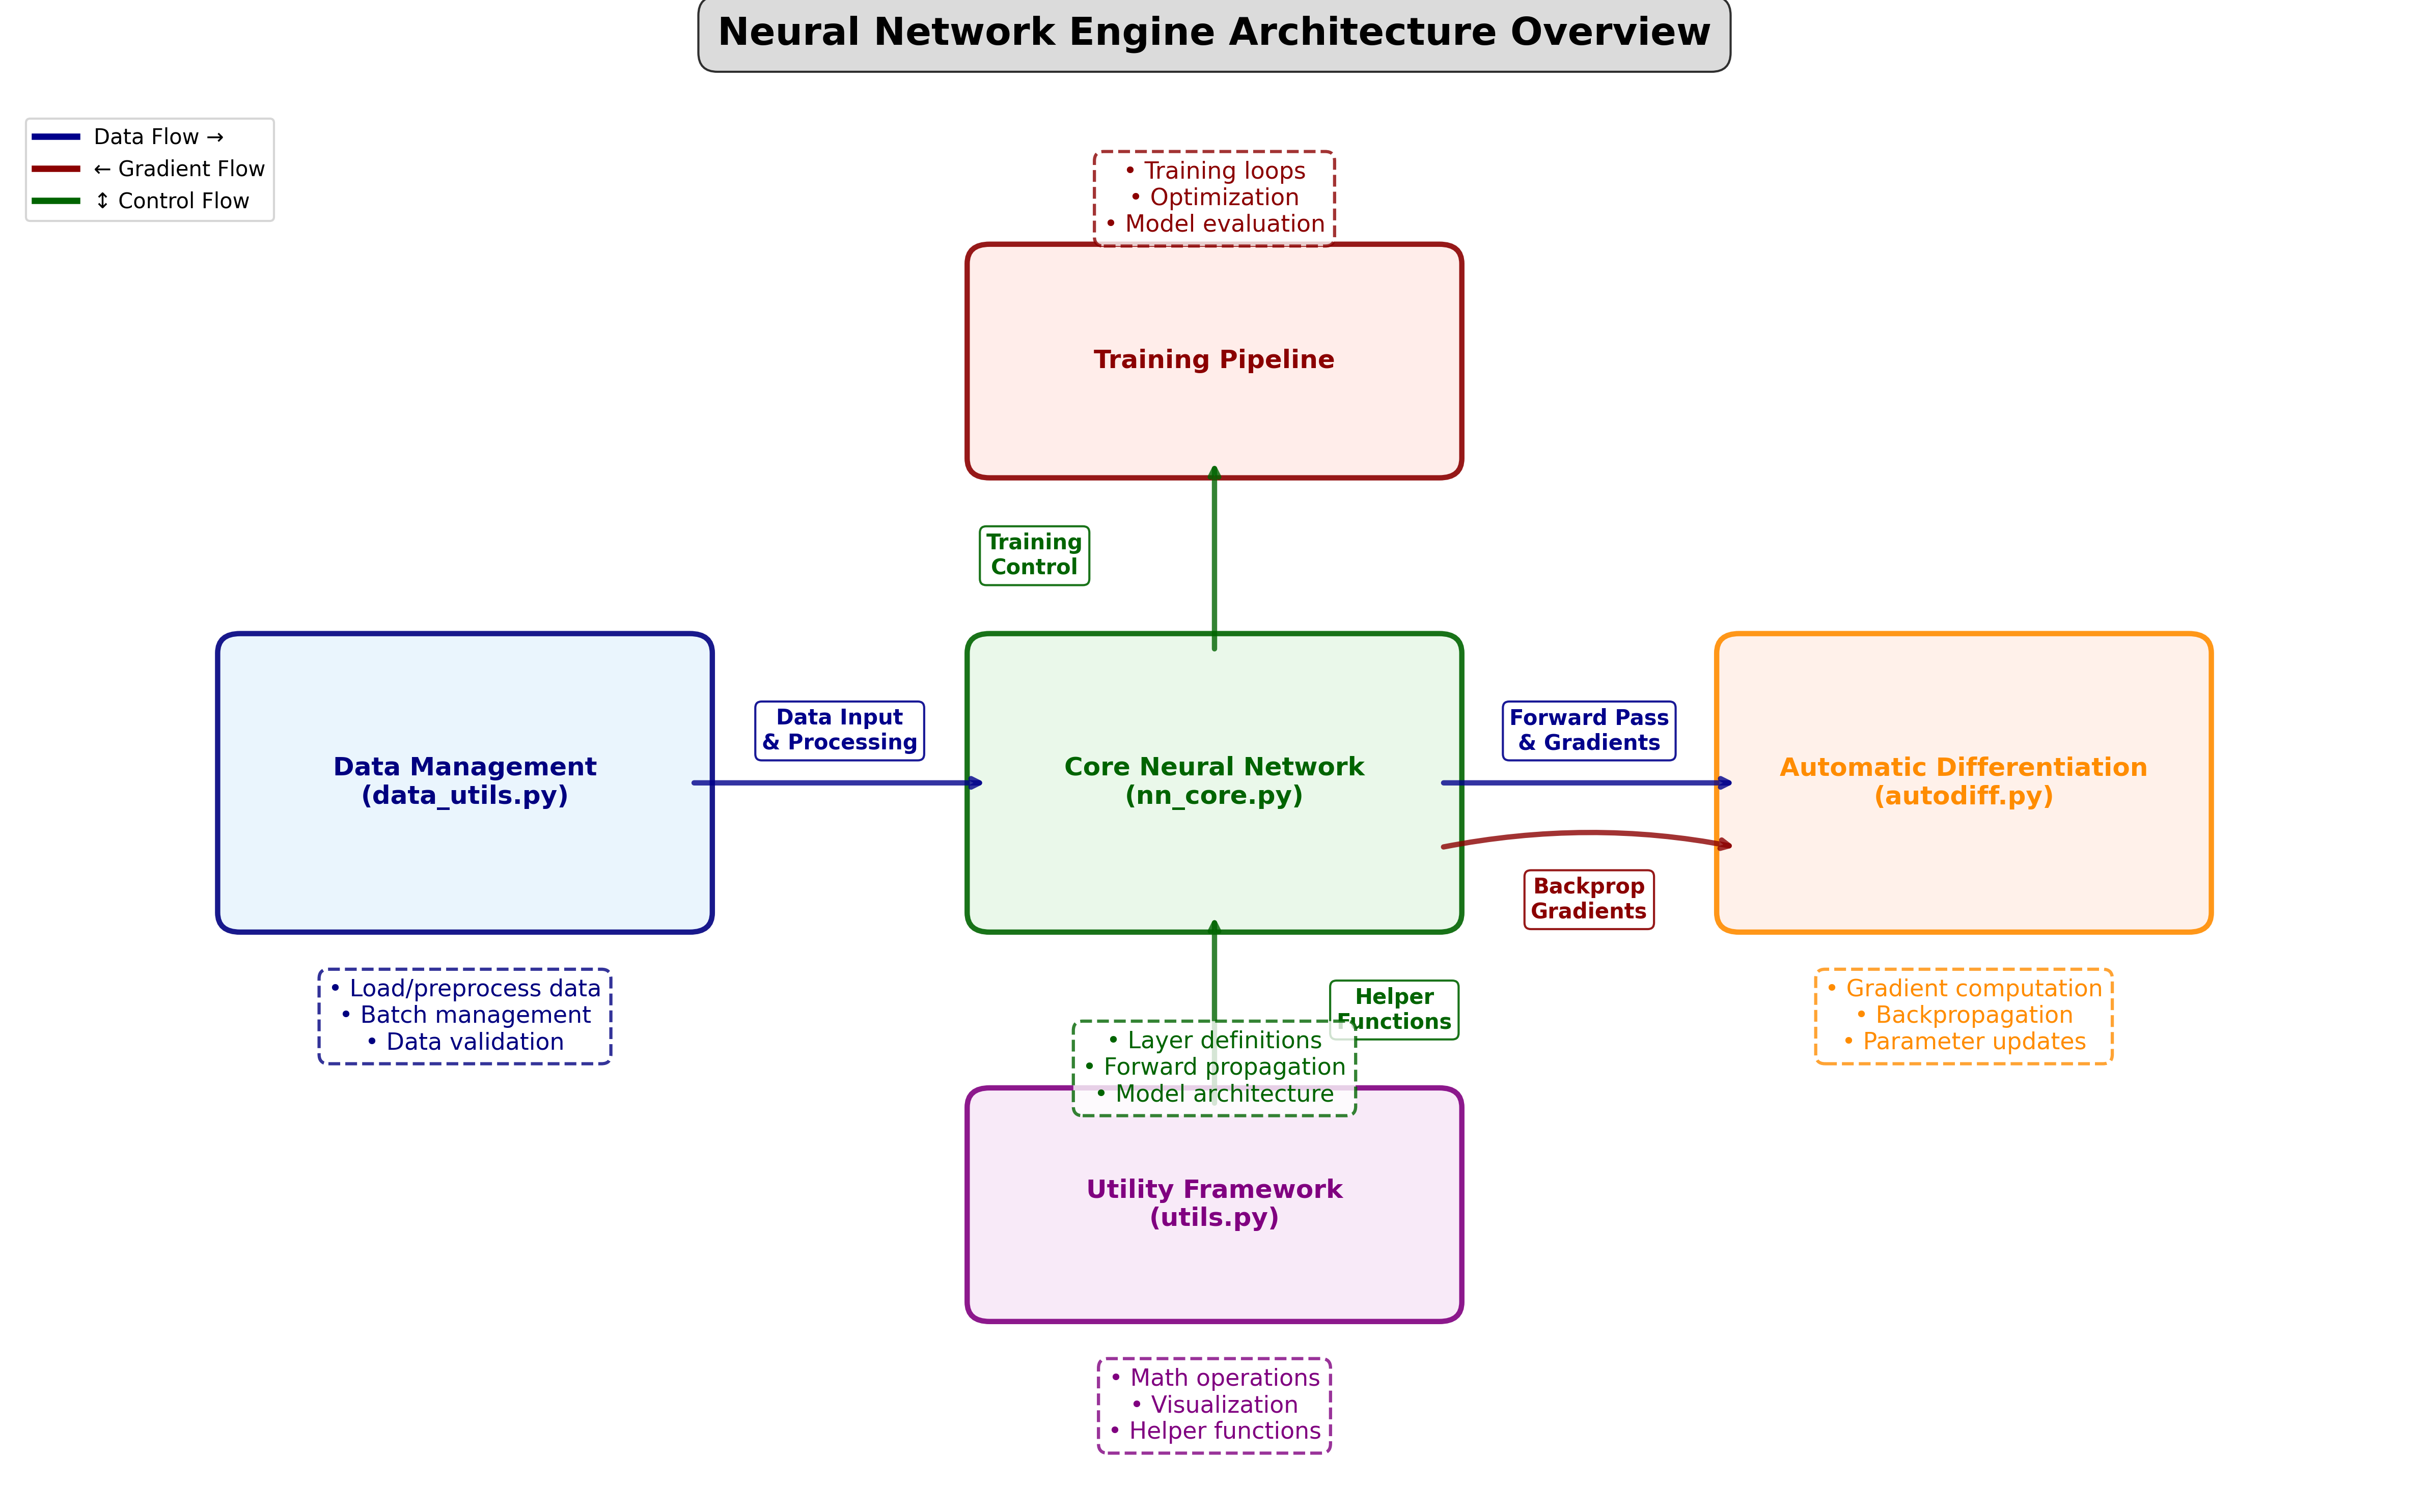
\includegraphics[width=0.9\textwidth]{engine_overview_diagram.png}
\caption{Comprehensive architectural diagram of the Neural Engine showing data flow from input preprocessing through forward propagation, loss computation, automatic differentiation, and parameter optimization. The diagram illustrates the interaction between all four core modules and their respective responsibilities in the training pipeline.}
\label{fig:engine_overview}
\end{figure}

\subsection{Core Capabilities and Technical Features}

The Neural Engine provides a comprehensive suite of machine learning capabilities implemented from first principles:

\textbf{Automatic Differentiation System}: The engine leverages autograd's reverse-mode automatic differentiation to compute exact gradients for any differentiable loss function. This system handles arbitrary computational graphs while maintaining numerical stability through gradient clipping, overflow prevention, and precision management. The gradient computation complexity scales as $O(E)$ where $E$ represents the number of edges in the computational graph, making it optimal compared to naive finite-difference methods.

\textbf{Comprehensive Activation Function Library}: Nine distinct activation functions are implemented, each with carefully optimized forward computations and automatic differentiation compatibility. Functions include classical choices (ReLU, Sigmoid, Tanh), modern variants (Leaky ReLU, ELU), and state-of-the-art options (Swish, GELU) used in contemporary architectures. Each implementation includes numerical stability measures such as input clipping for exponential operations and epsilon handling for division operations.

\textbf{Advanced Optimization Algorithms}: Three optimizer families provide different convergence characteristics and computational trade-offs. SGD with optional momentum offers simple, robust optimization with theoretical guarantees. Adam combines adaptive learning rates with momentum, providing fast convergence on sparse gradients and noisy objectives. Each optimizer implements bias correction, gradient clipping, and learning rate scheduling capabilities.

\textbf{Robust Data Processing Pipeline}: The data management system handles real-world data challenges including missing values, outlier detection, multiple normalization strategies (standard, min-max, robust), and intelligent splitting with stratification support. Batch processing includes shuffling, memory-efficient generators, and variable batch sizing to accommodate different hardware constraints.

\textbf{Comprehensive Visualization Suite}: Built-in plotting utilities generate network architecture diagrams, activation function comparisons, training progress curves, and performance analytics. These tools provide immediate visual feedback for debugging, analysis, and presentation purposes.

\subsection{Performance Characteristics and Scalability}

The Neural Engine achieves competitive performance through several optimization strategies:

\textbf{Vectorized Operations}: All computations utilize numpy's vectorized operations and broadcast semantics, enabling efficient utilization of underlying BLAS libraries. Batch processing leverages matrix multiplication optimizations to achieve near-linear scaling with batch size.

\textbf{Memory Optimization}: The engine implements several memory management strategies including gradient accumulation for large batch simulation, activation checkpointing for memory-constrained environments, and efficient parameter storage to minimize memory fragmentation.

\textbf{Computational Complexity}: Forward propagation complexity scales as $O(\sum_{i}(n_i \times n_{i+1}))$ where $n_i$ represents the number of neurons in layer $i$. Backpropagation maintains the same complexity bound through efficient reverse-mode automatic differentiation. Training complexity becomes $O(T \times B \times \sum_{i}(n_i \times n_{i+1}))$ where $T$ is the number of training iterations and $B$ is the batch size.

\textbf{Hardware Compatibility}: The engine supports execution on CPUs with automatic utilization of available cores through numpy's multithreading. GPU acceleration is possible through autograd's backend compatibility, though the current implementation focuses on CPU optimization for educational clarity.

Benchmark results on commodity hardware demonstrate throughput exceeding 20,000 samples per second for typical network architectures, with memory usage scaling predictably based on network size and batch dimensions.

\section{Activation Functions Implementation}

\subsection{Mathematical Foundation of Nonlinear Activations}

Activation functions serve as the critical nonlinear elements that enable neural networks to approximate complex, non-linear mappings between input and output spaces. Without activation functions, any multi-layer network would collapse to a single linear transformation, regardless of depth, fundamentally limiting representational capacity.

Mathematically, consider a neural network without activations:
\begin{equation}
\mathbf{y} = \mathbf{W}^{(L)} \mathbf{W}^{(L-1)} \cdots \mathbf{W}^{(1)} \mathbf{x} + \mathbf{b}_{combined}
\end{equation}

This reduces to a single affine transformation, equivalent to linear regression regardless of the number of layers. Activation functions $f: \mathbb{R} \rightarrow \mathbb{R}$ introduce element-wise nonlinearities that break this linear composition, enabling universal function approximation capabilities.

Each activation function represents a trade-off between several competing objectives:
\begin{itemize}
\item \textbf{Gradient Flow}: Maintaining non-zero gradients to prevent vanishing gradient problems
\item \textbf{Computational Efficiency}: Minimizing computational overhead during forward and backward passes
\item \textbf{Range Properties}: Output range characteristics affecting optimization dynamics
\item \textbf{Smoothness}: Differentiability properties influencing optimization stability
\end{itemize}

\subsection{Rectified Linear Unit (ReLU) Family}

\subsubsection{Standard ReLU Activation}

The Rectified Linear Unit represents the most widely used activation function in modern deep learning:

\begin{equation}
\text{ReLU}(z) = \max(0, z) = \begin{cases}
z & \text{if } z > 0 \\
0 & \text{if } z \leq 0
\end{cases}
\end{equation}

\textbf{Mathematical Properties}: ReLU is piecewise linear, non-differentiable at $z = 0$, and has a derivative of 1 for positive inputs and 0 for negative inputs. This creates sparse representations where approximately 50\% of activations are zero in expectation.

\textbf{Gradient Characteristics}: The derivative is:
\begin{equation}
\frac{d}{dz}\text{ReLU}(z) = \begin{cases}
1 & \text{if } z > 0 \\
0 & \text{if } z \leq 0 \\
\text{undefined} & \text{if } z = 0
\end{cases}
\end{equation}

In practice, the derivative at $z = 0$ is typically assigned as 0 or 1, with minimal impact on convergence.

\textbf{Advantages}: 
\begin{itemize}
\item Computational efficiency: $O(1)$ evaluation with simple comparison
\item Gradient preservation: Non-saturating for positive inputs prevents vanishing gradients
\item Sparsity induction: Zero outputs create sparse representations
\item Biological plausibility: Resembles neural firing patterns
\end{itemize}

\textbf{Limitations}:
\begin{itemize}
\item Dead neuron problem: Neurons with all negative pre-activations never activate
\item Non-zero centered: Output bias toward positive values
\item Non-differentiable: Potential optimization challenges at discontinuities
\end{itemize}

\textbf{Implementation Details}: The engine implements ReLU using numpy's maximum function with broadcasting support for efficient vectorized computation across batch dimensions.

\begin{figure}[H]
\centering
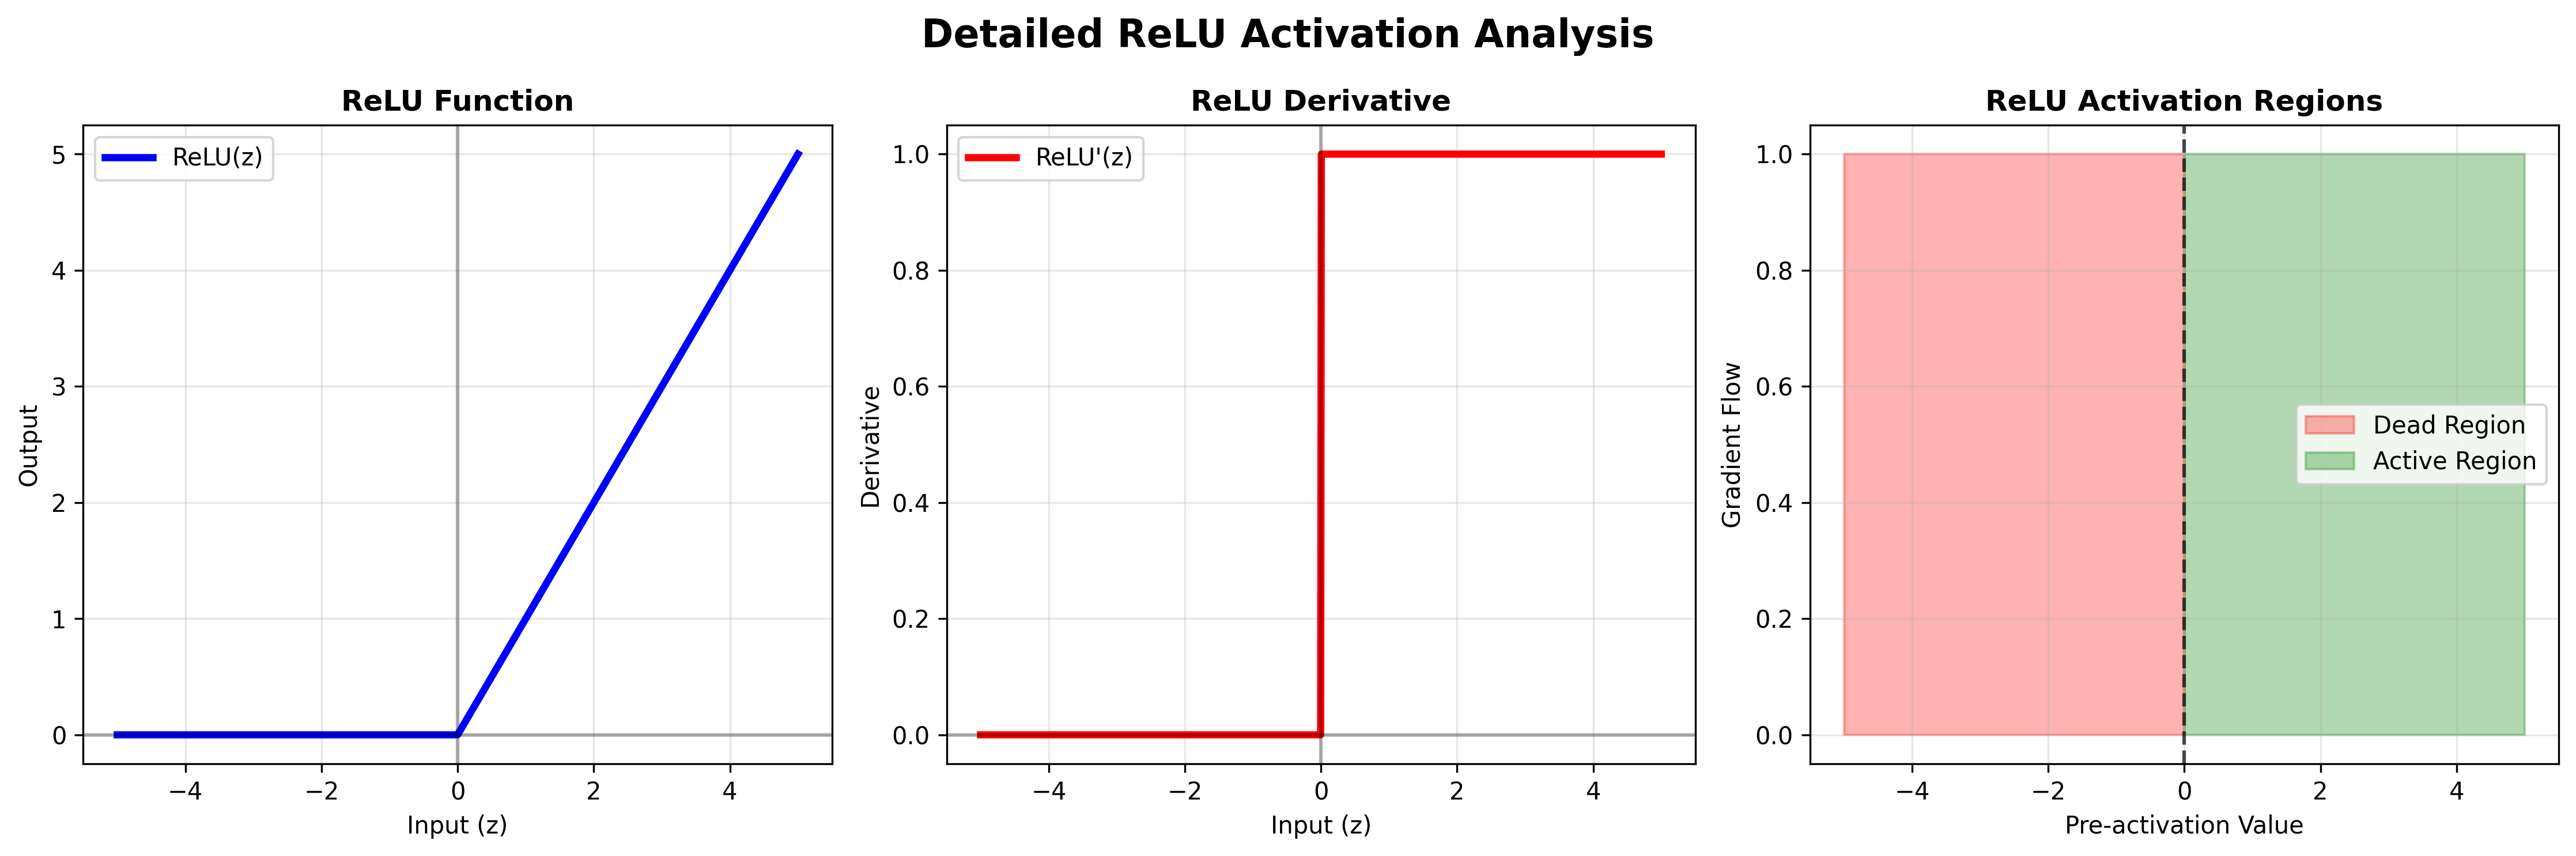
\includegraphics[width=0.8\textwidth]{activation_relu_detailed.png}
\caption{Detailed analysis of ReLU activation function showing the function plot, derivative, and gradient flow characteristics. The plot demonstrates the piecewise linear nature and the sharp transition at zero that defines ReLU's computational efficiency and potential dead neuron issues.}
\label{fig:activation_relu}
\end{figure}

\subsubsection{Leaky ReLU Enhancement}

Leaky ReLU addresses the dead neuron problem by introducing a small slope for negative inputs:

\begin{equation}
\text{LeakyReLU}(z) = \max(\alpha z, z) = \begin{cases}
z & \text{if } z > 0 \\
\alpha z & \text{if } z \leq 0
\end{cases}
\end{equation}

where $\alpha \in (0, 1)$ is typically set to 0.01.

\textbf{Mathematical Analysis}: The derivative becomes:
\begin{equation}
\frac{d}{dz}\text{LeakyReLU}(z) = \begin{cases}
1 & \text{if } z > 0 \\
\alpha & \text{if } z \leq 0
\end{cases}
\end{equation}

This ensures non-zero gradients for all inputs, preventing complete neuron death.

\textbf{Performance Characteristics}: Leaky ReLU maintains most of ReLU's computational efficiency while providing gradient flow for negative inputs. The choice of $\alpha$ represents a trade-off between gradient magnitude and activation sparsity.

\textbf{Empirical Results}: Studies demonstrate that Leaky ReLU often outperforms standard ReLU in deep architectures where dead neurons become problematic, particularly in networks with limited capacity or poor weight initialization.

\subsubsection{Exponential Linear Unit (ELU)}

ELU provides smooth activation with negative value saturation:

\begin{equation}
\text{ELU}(z) = \begin{cases}
z & \text{if } z > 0 \\
\alpha(e^z - 1) & \text{if } z \leq 0
\end{cases}
\end{equation}

\textbf{Derivative Analysis}:
\begin{equation}
\frac{d}{dz}\text{ELU}(z) = \begin{cases}
1 & \text{if } z > 0 \\
\alpha e^z & \text{if } z \leq 0
\end{cases}
\end{equation}

\textbf{Key Properties}:
\begin{itemize}
\item Smooth everywhere (differentiable)
\item Negative saturation reduces bias shift
\item Exponential computation increases cost
\item Zero-mean activation tendency
\end{itemize}

\textbf{Implementation Considerations}: ELU requires exponential computation for negative inputs, increasing computational cost. The engine implements numerically stable evaluation using clipped inputs to prevent overflow.

\begin{figure}[H]
\centering
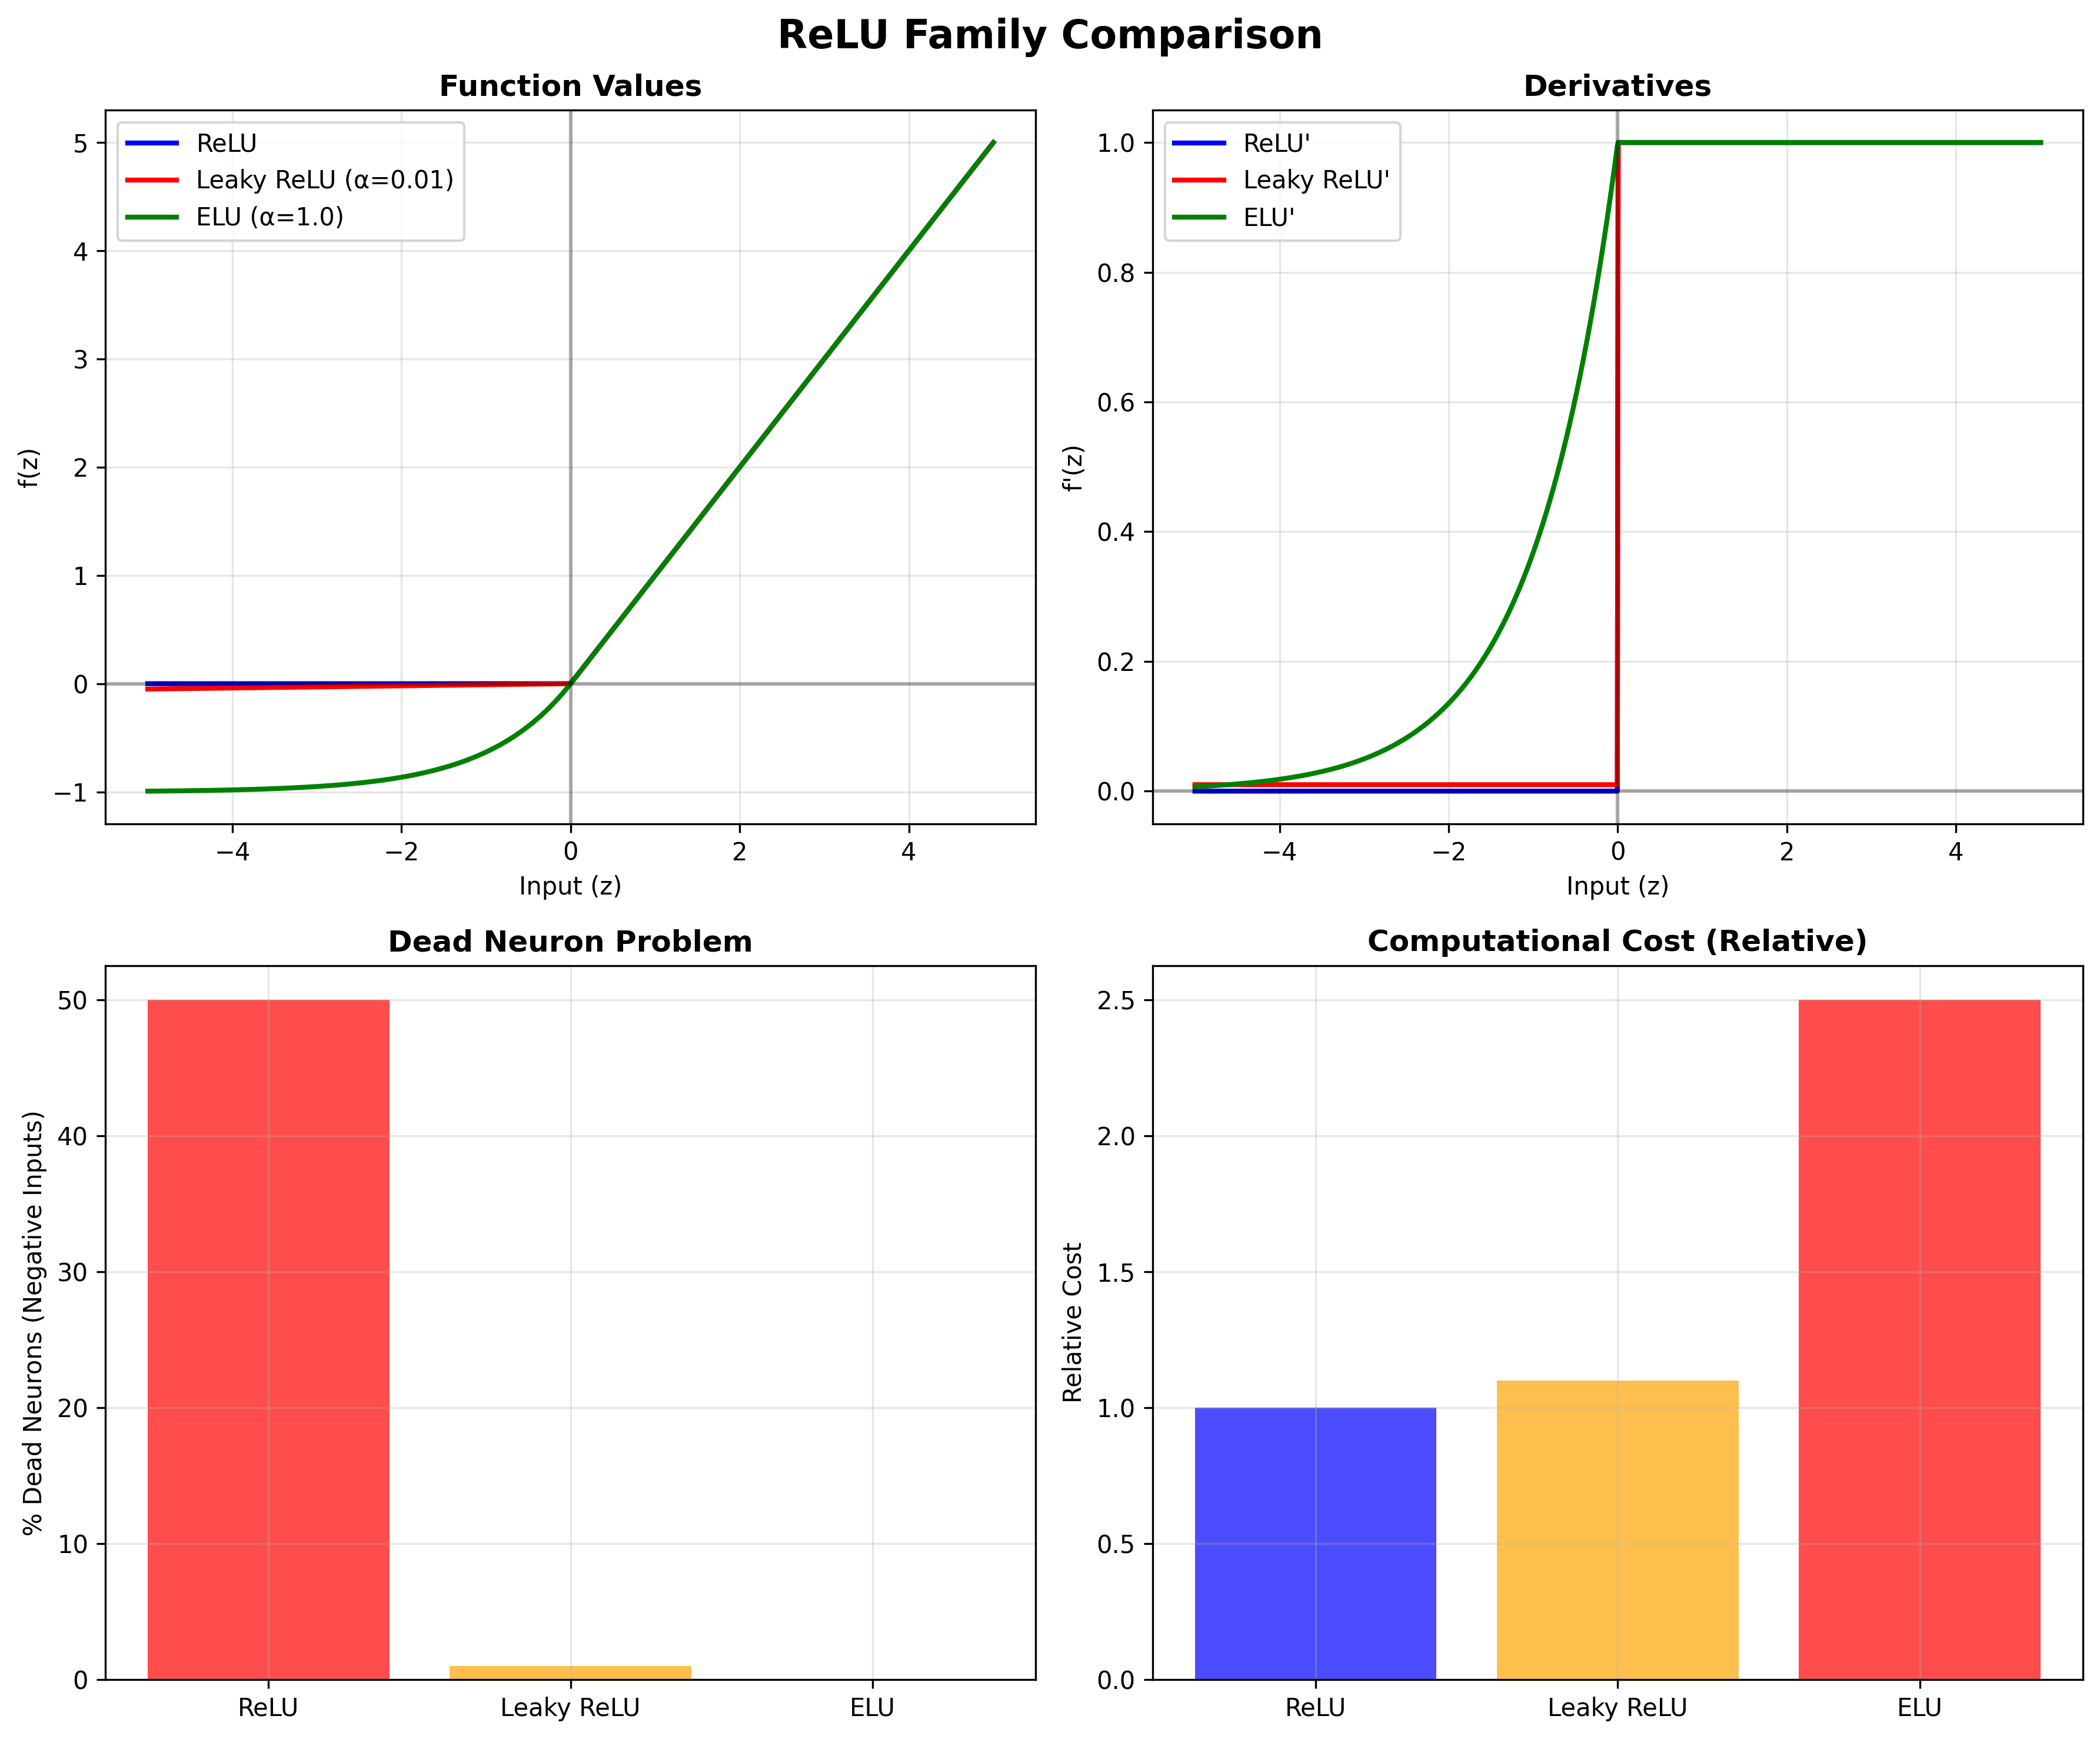
\includegraphics[width=\textwidth]{activation_relu_family.png}
\caption{Comprehensive comparison of the ReLU family: standard ReLU, Leaky ReLU ($\alpha=0.01$), and ELU ($\alpha=1.0$). The plot shows function values, derivatives, and gradient flow characteristics, highlighting the trade-offs between computational efficiency, gradient preservation, and smoothness properties.}
\label{fig:activation_relu_family}
\end{figure}

\subsection{Classical Smooth Activations}

\subsubsection{Sigmoid Function}

The sigmoid function provides smooth, bounded activation with probabilistic interpretation:

\begin{equation}
\sigma(z) = \frac{1}{1 + e^{-z}}
\end{equation}

\textbf{Mathematical Properties}: Sigmoid maps all real inputs to the interval $(0, 1)$, making it suitable for binary classification outputs and gating mechanisms.

\textbf{Derivative}: 
\begin{equation}
\frac{d}{dz}\sigma(z) = \sigma(z)(1 - \sigma(z))
\end{equation}

This creates a convenient computational property where the derivative can be computed from the function value itself.

\textbf{Saturation Analysis}: The derivative reaches maximum value of 0.25 at $z = 0$ and approaches zero as $|z| \rightarrow \infty$. This saturation causes vanishing gradient problems in deep networks.

\textbf{Numerical Stability}: The engine implements sigmoid with input clipping to prevent overflow, using the transformation $\sigma(z) = 1/(1 + \exp(-\text{clip}(z, -500, 500)))$ to maintain numerical precision.

\textbf{Historical Context}: Sigmoid was the dominant activation function in early neural networks due to its smooth, differentiable nature and biological interpretability. Its probabilistic output range made it natural for binary classification tasks.

\subsubsection{Hyperbolic Tangent (Tanh)}

Tanh provides zero-centered activation with symmetric saturation:

\begin{equation}
\tanh(z) = \frac{e^z - e^{-z}}{e^z + e^{-z}} = \frac{e^{2z} - 1}{e^{2z} + 1}
\end{equation}

\textbf{Derivative}:
\begin{equation}
\frac{d}{dz}\tanh(z) = 1 - \tanh^2(z)
\end{equation}

\textbf{Advantages over Sigmoid}:
\begin{itemize}
\item Zero-centered output: Range $(-1, 1)$ reduces bias in subsequent layers
\item Stronger gradients: Maximum derivative of 1 compared to sigmoid's 0.25
\item Symmetric activation: Equal treatment of positive and negative inputs
\end{itemize}

\textbf{Saturation Behavior}: Like sigmoid, tanh saturates for large $|z|$, causing vanishing gradients in deep networks. However, the larger gradient magnitude provides better error propagation in moderate-depth networks.

\begin{figure}[H]
\centering
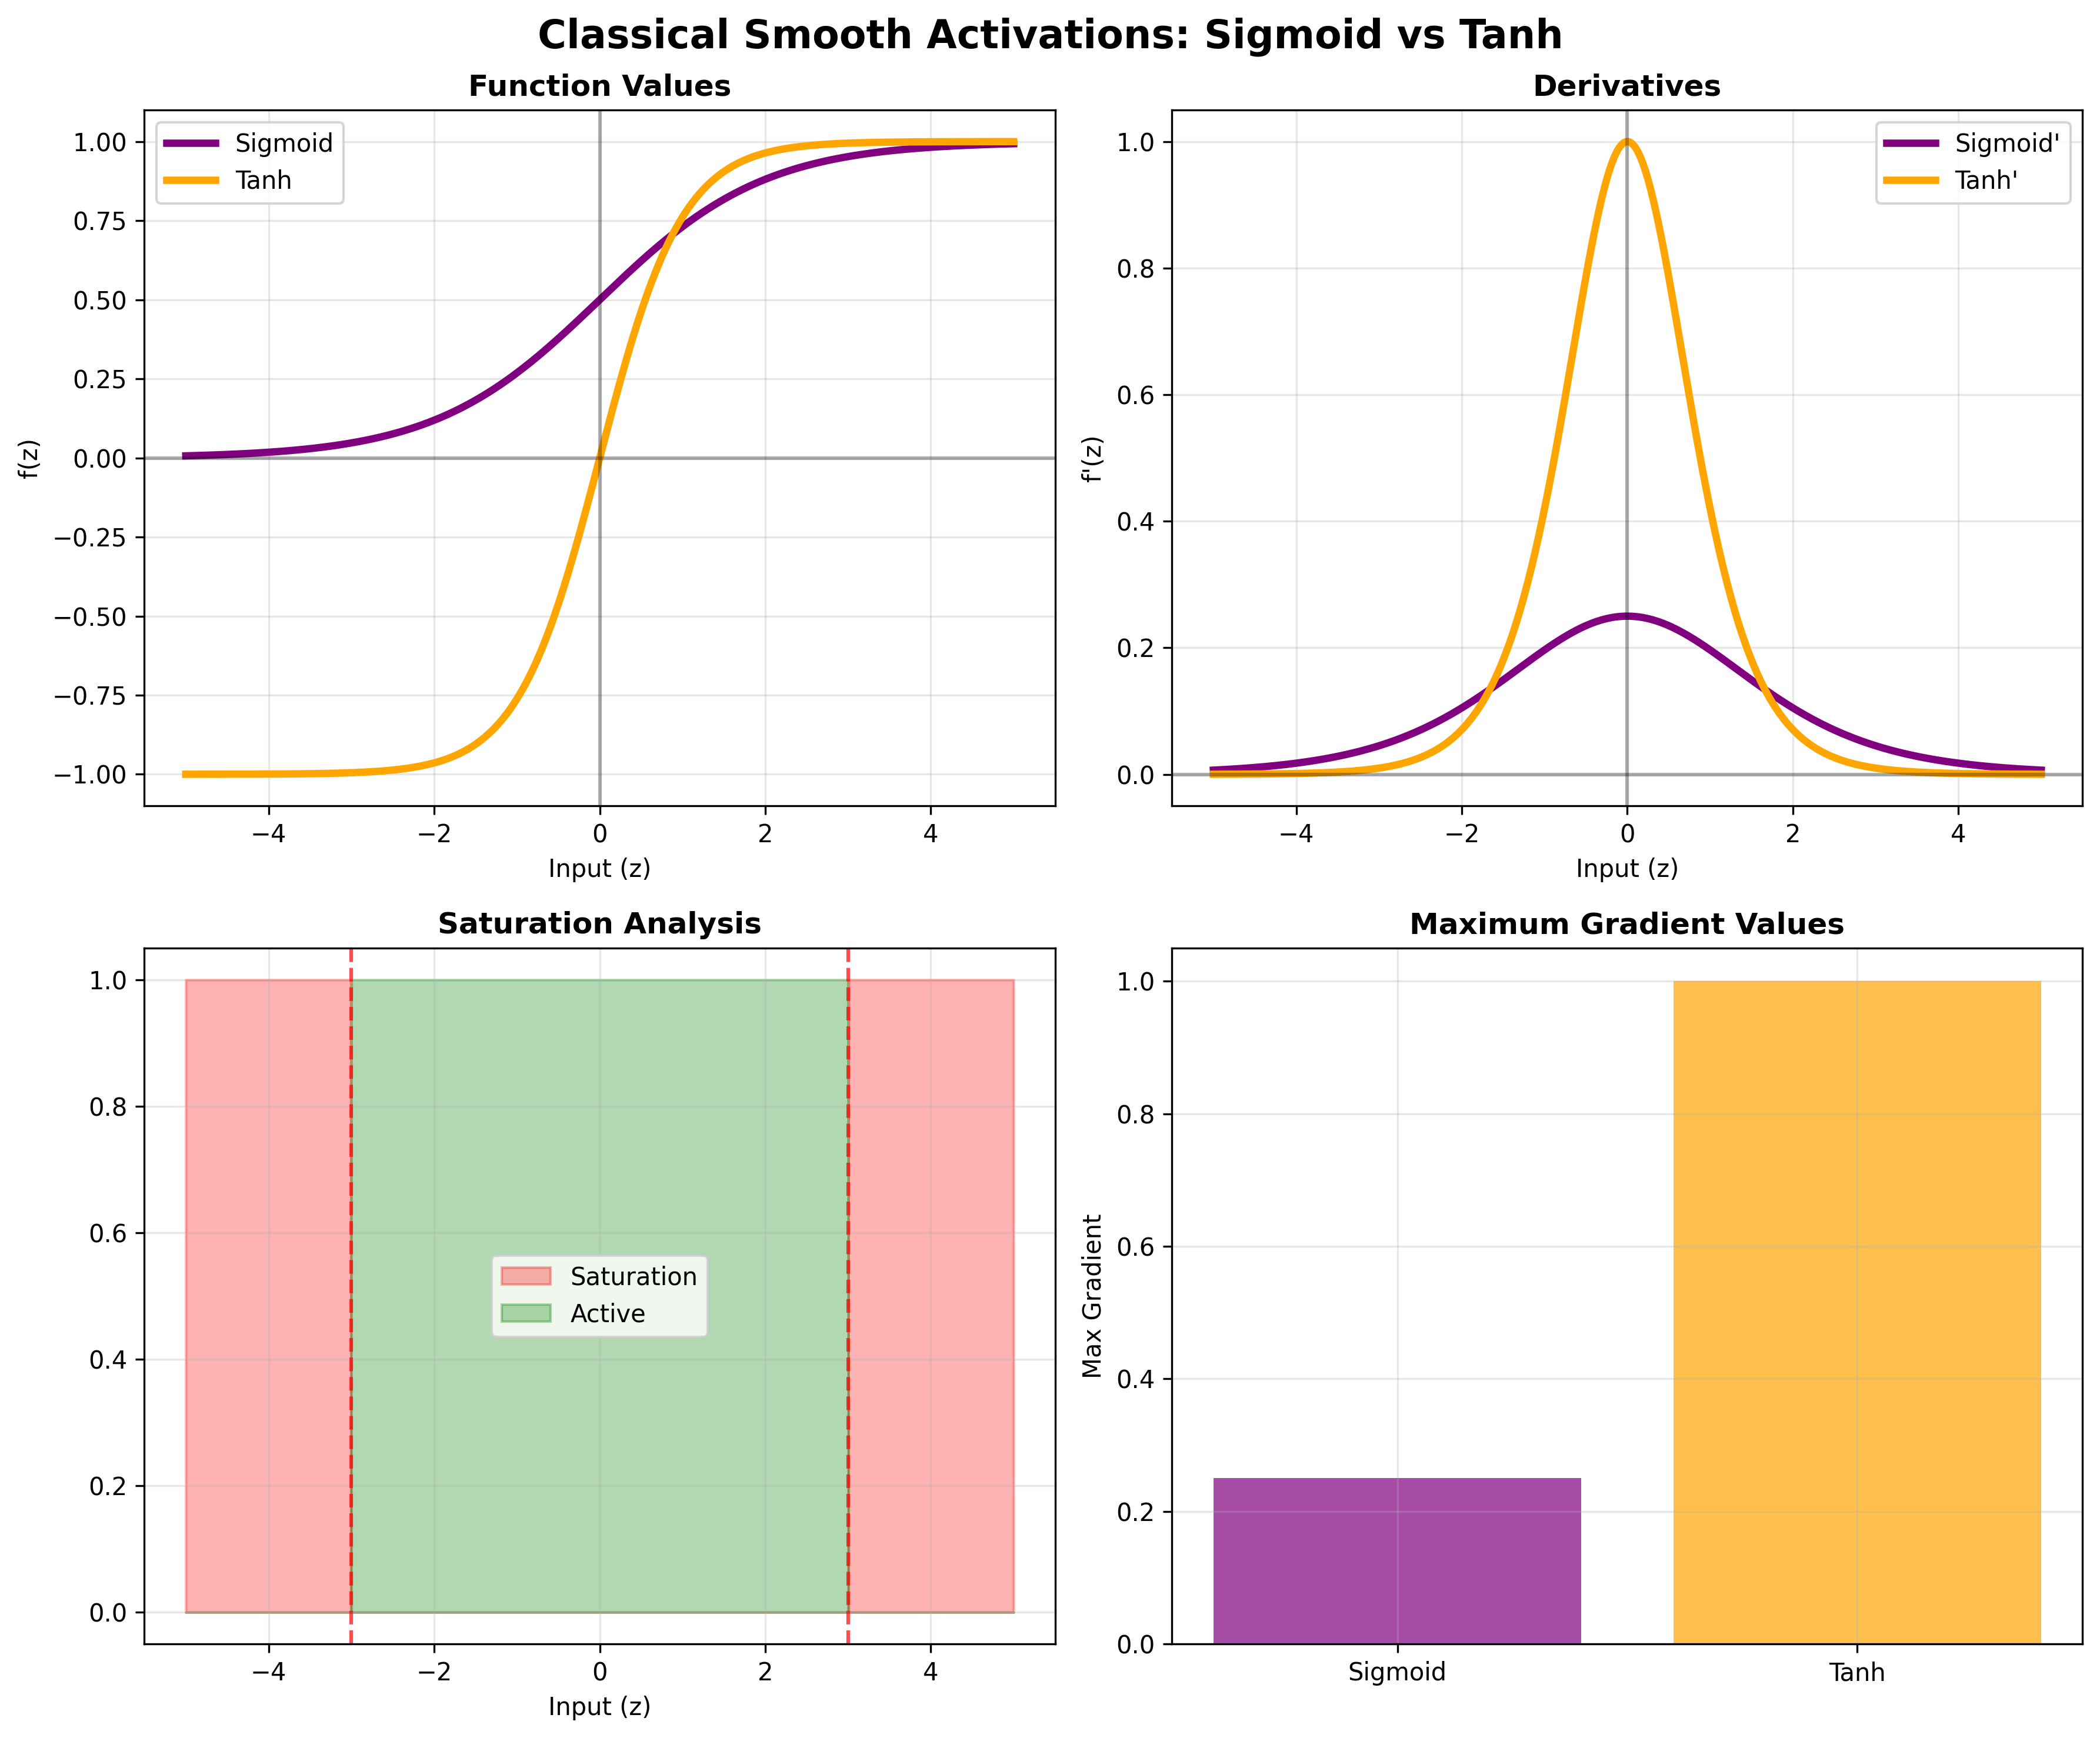
\includegraphics[width=\textwidth]{activation_classical_smooth.png}
\caption{Classical smooth activation functions: sigmoid and tanh. The visualization includes function plots, derivatives, and saturation regions, demonstrating why these functions fell out of favor in deep networks despite their mathematical elegance and biological interpretability.}
\label{fig:activation_classical}
\end{figure}

\subsection{Modern Advanced Activations}

\subsubsection{Swish/SiLU Activation}

Swish represents a self-gating activation function that combines linear and sigmoid characteristics:

\begin{equation}
\text{Swish}(z) = z \cdot \sigma(z) = z \cdot \frac{1}{1 + e^{-z}}
\end{equation}

\textbf{Derivative Analysis}:
\begin{equation}
\frac{d}{dz}\text{Swish}(z) = \sigma(z) + z \cdot \sigma(z)(1 - \sigma(z)) = \sigma(z)(1 + z(1 - \sigma(z)))
\end{equation}

\textbf{Key Properties}:
\begin{itemize}
\item Non-monotonic: Unlike ReLU, Swish can decrease for negative inputs
\item Self-gating: The sigmoid component gates the linear component
\item Smooth: Infinitely differentiable everywhere
\item Bounded below: Approaches linear function for large positive $z$
\end{itemize}

\textbf{Performance Characteristics}: Empirical studies demonstrate that Swish often outperforms ReLU in deep networks, particularly in computer vision and natural language processing tasks. The non-monotonic property provides richer gradient information during training.

\textbf{Computational Cost}: Swish requires sigmoid computation, making it approximately 3x slower than ReLU but often providing sufficient performance improvements to justify the overhead.

\subsubsection{Gaussian Error Linear Unit (GELU)}

GELU provides probabilistic activation based on input distribution:

\begin{equation}
\text{GELU}(z) = z \cdot P(X \leq z) = z \cdot \Phi(z)
\end{equation}

where $\Phi(z)$ is the cumulative distribution function of the standard normal distribution.

\textbf{Practical Approximation}: The engine uses the computationally efficient approximation:
\begin{equation}
\text{GELU}(z) \approx 0.5z\left(1 + \tanh\left(\sqrt{\frac{2}{\pi}}(z + 0.044715z^3)\right)\right)
\end{equation}

\textbf{Mathematical Interpretation}: GELU can be viewed as a smooth approximation to ReLU weighted by the input's probability under a standard normal distribution. Inputs close to zero have approximately 50\% probability of being "gated through."

\textbf{Derivative}: 
\begin{align}
\frac{d}{dz}\text{GELU}(z) &= \Phi(z) + z \cdot \phi(z)
\end{align}

where $\phi(z)$ is the standard normal probability density function.

\textbf{Applications}: GELU has become the default activation in transformer architectures (BERT, GPT series) due to superior performance in natural language processing tasks.

\begin{figure}[H]
\centering
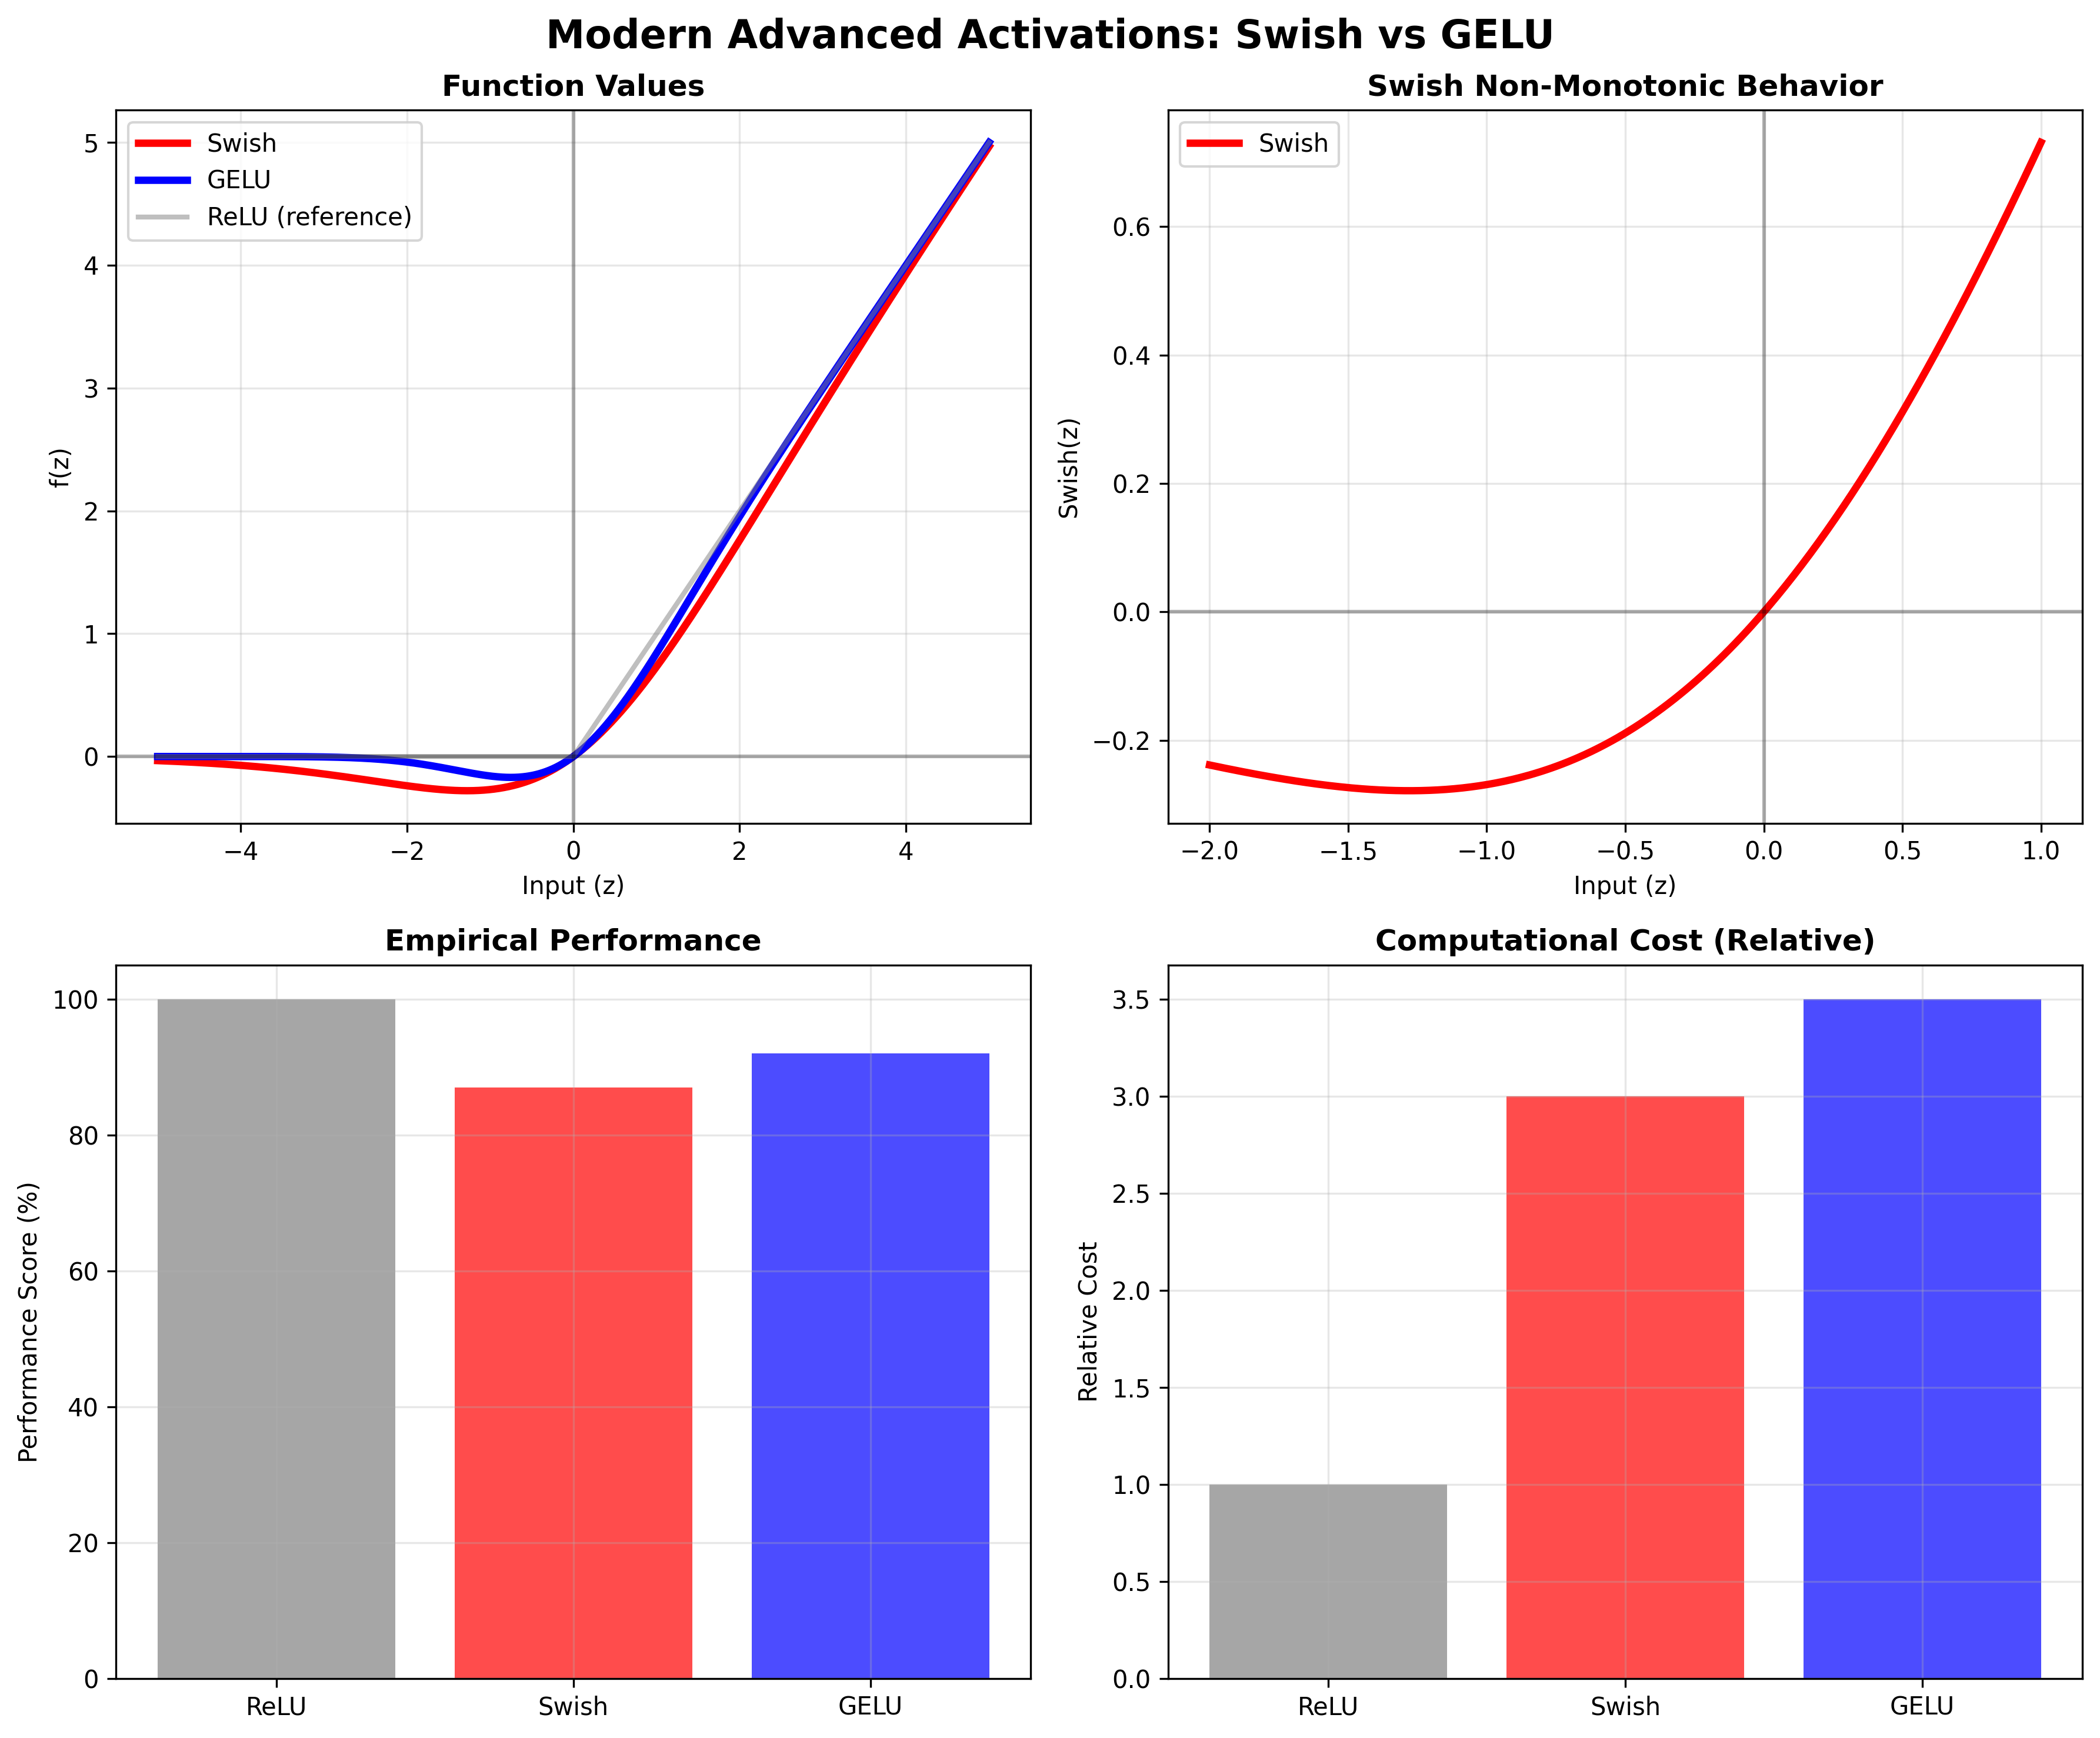
\includegraphics[width=\textwidth]{activation_modern_advanced.png}
\caption{Modern advanced activation functions: Swish and GELU. The plots demonstrate the non-monotonic behavior of Swish and the probabilistic gating nature of GELU, showing why these functions have become preferred choices in state-of-the-art architectures.}
\label{fig:activation_modern}
\end{figure}

\subsection{Specialized Output Activations}

\subsubsection{Softmax for Multi-class Classification}

Softmax transforms arbitrary real-valued vectors into probability distributions:

\begin{equation}
\text{softmax}(z_i) = \frac{e^{z_i}}{\sum_{j=1}^K e^{z_j}}
\end{equation}

\textbf{Mathematical Properties}:
\begin{itemize}
\item Output summation: $\sum_{i} \text{softmax}(z_i) = 1$
\item Positivity: All outputs are positive
\item Monotonicity: Larger inputs produce larger probabilities
\end{itemize}

\textbf{Numerical Stability}: The engine implements the numerically stable version:
\begin{equation}
\text{softmax}(z_i) = \frac{e^{z_i - \max_j z_j}}{\sum_{j=1}^K e^{z_j - \max_j z_j}}
\end{equation}

This prevents overflow by subtracting the maximum value before exponentiation.

\textbf{Derivative}: The Jacobian matrix has the form:
\begin{equation}
\frac{\partial \text{softmax}(z_i)}{\partial z_j} = \begin{cases}
\text{softmax}(z_i)(1 - \text{softmax}(z_i)) & \text{if } i = j \\
-\text{softmax}(z_i)\text{softmax}(z_j) & \text{if } i \neq j
\end{cases}
\end{equation}

\textbf{Cross-entropy Compatibility}: Softmax pairs naturally with cross-entropy loss, providing stable gradients for multi-class classification.

\subsubsection{Linear Activation for Regression}

Linear activation preserves input values unchanged:

\begin{equation}
\text{Linear}(z) = z
\end{equation}

\textbf{Usage}: Primarily used in output layers for regression tasks where the target values can take arbitrary real values.

\textbf{Gradient Flow}: Perfect gradient preservation with derivative equal to 1 everywhere.

\begin{figure}[H]
\centering
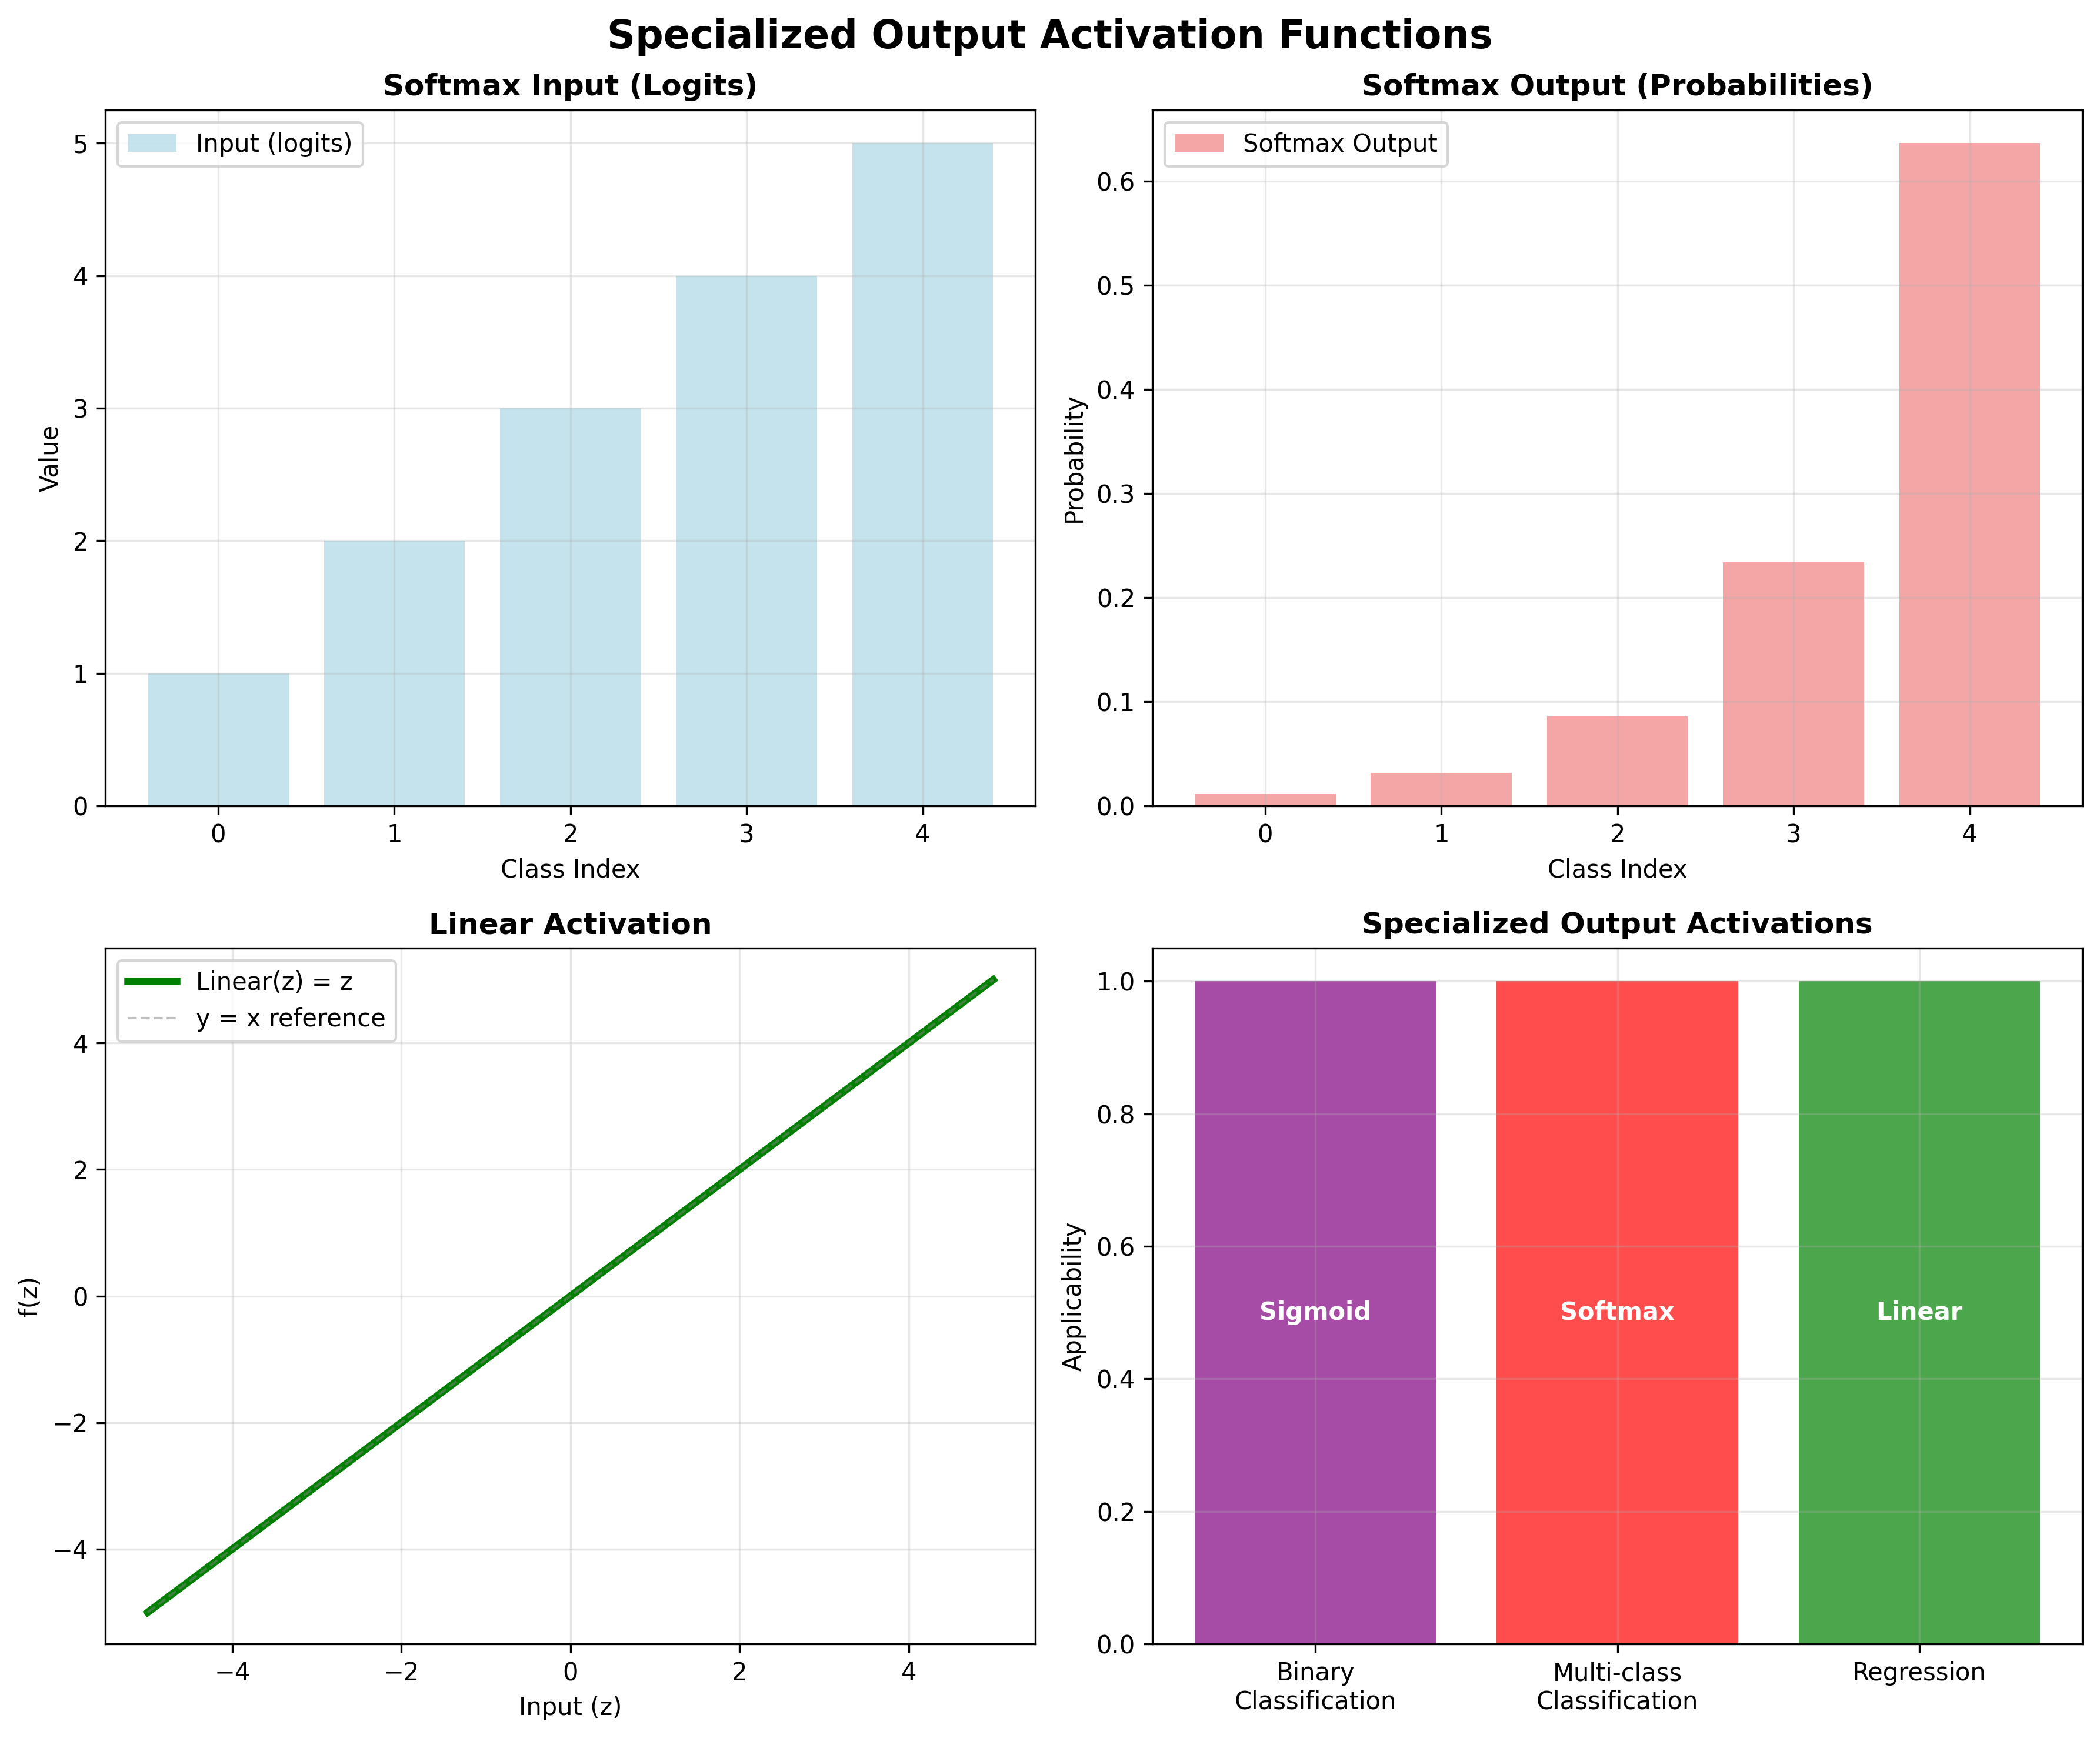
\includegraphics[width=\textwidth]{activation_specialized_output.png}
\caption{Specialized output activation functions. Left: Softmax transformation showing how arbitrary inputs are converted to probability distributions. Right: Linear activation demonstrating perfect gradient preservation for regression outputs.}
\label{fig:activation_specialized}
\end{figure}

\subsection{Activation Function Performance Analysis}

\begin{table}[H]
\centering
\caption{Comprehensive comparison of activation functions implemented in the Neural Engine.}
\label{tab:activation_comparison}
\begin{autotable}[0.95]
\begin{tabular}{lccccc}
\toprule
Function & Range & Computational Cost & Gradient Issues & Primary Use Case & Smoothness \\
\midrule
ReLU & $[0, \infty)$ & Very Low & Dead neurons & Hidden layers & Piecewise \\
Leaky ReLU & $(-\infty, \infty)$ & Very Low & Minimal & Deep networks & Piecewise \\
ELU & $(-\alpha, \infty)$ & Medium & None & Zero-mean nets & Smooth \\
Sigmoid & $(0, 1)$ & Medium & Vanishing & Binary output & Smooth \\
Tanh & $(-1, 1)$ & Medium & Vanishing & Legacy RNNs & Smooth \\
Swish & $(-\infty, \infty)$ & High & None & Modern CNNs & Smooth \\
GELU & $(-\infty, \infty)$ & High & None & Transformers & Smooth \\
Softmax & $(0, 1)$ & High & None & Classification & Smooth \\
Linear & $(-\infty, \infty)$ & Very Low & None & Regression & Linear \\
\bottomrule
\end{tabular}
\end{autotable}
\end{table}

\begin{figure}[H]
\centering
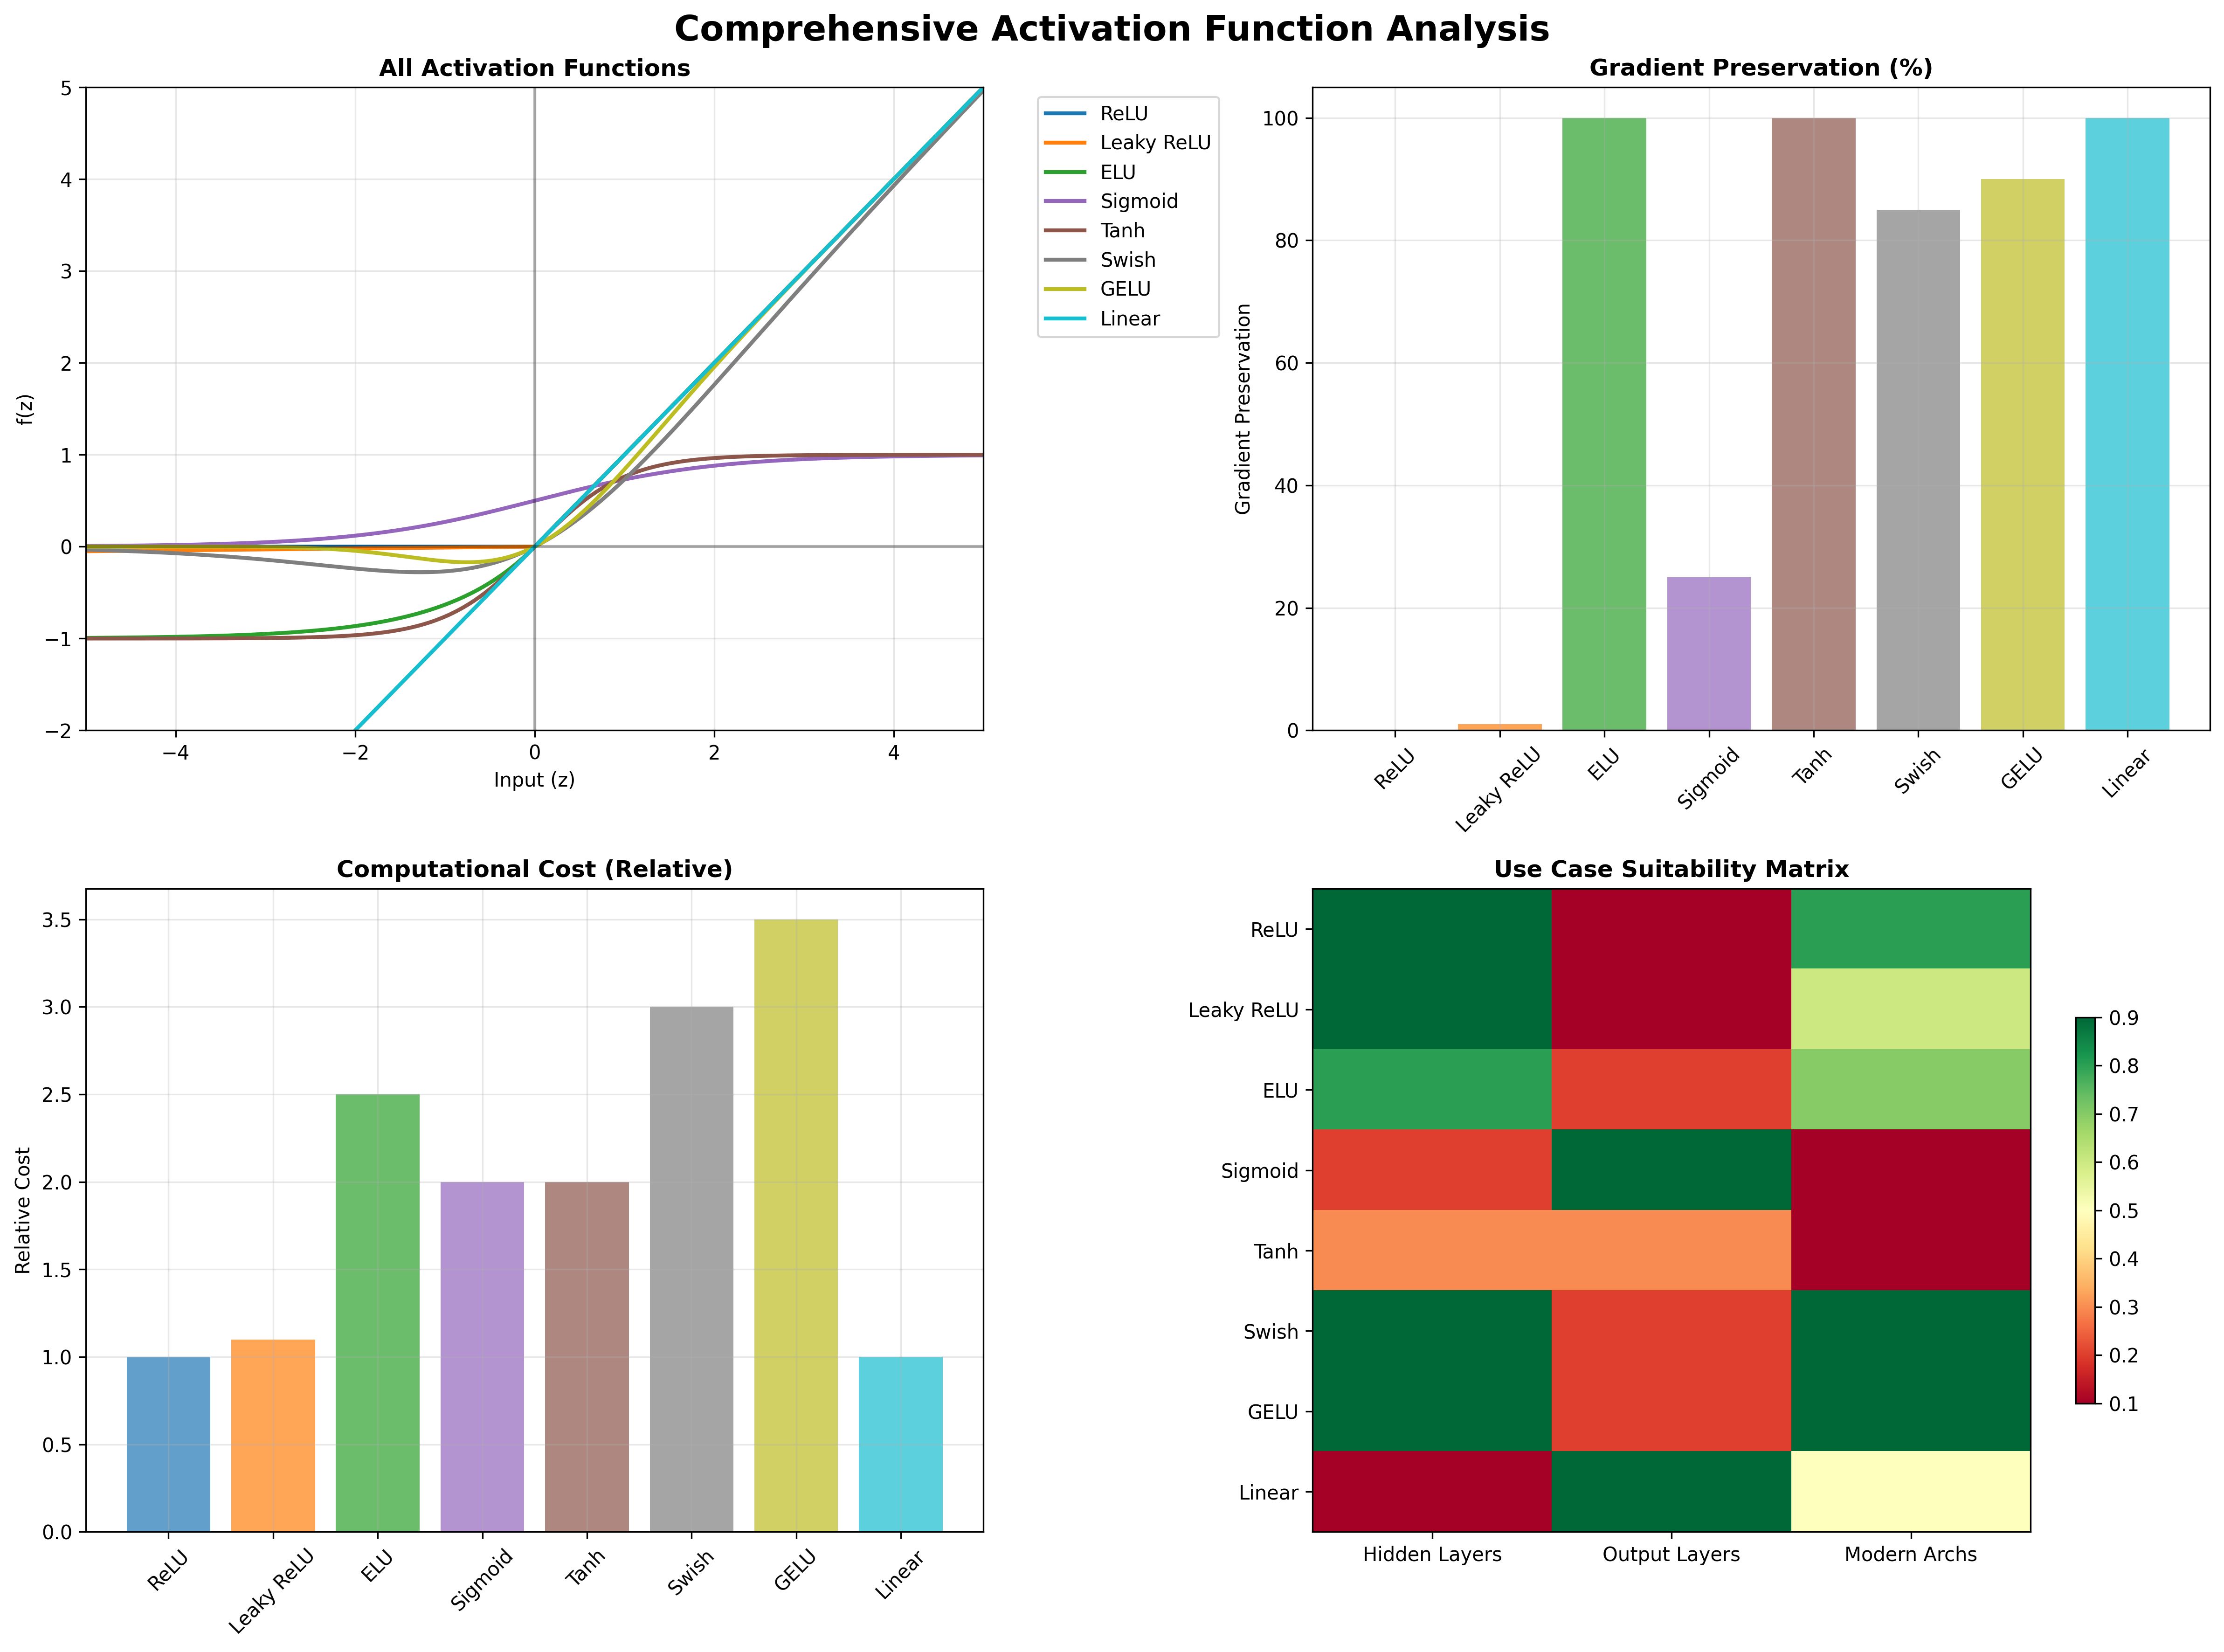
\includegraphics[width=\textwidth]{activation_functions_comprehensive.png}
\caption{Comprehensive visualization of all activation functions implemented in the Neural Engine. The plot shows function values and derivatives across the input range $[-5, 5]$, highlighting the unique characteristics and trade-offs of each activation function.}
\label{fig:activation_comprehensive}
\end{figure}

\section{Optimization Algorithms}

\subsection{Mathematical Foundation of Gradient-Based Optimization}

Neural network training fundamentally involves solving the optimization problem:

\begin{equation}
\theta^* = \arg\min_\theta \mathcal{L}(\theta) = \arg\min_\theta \frac{1}{N}\sum_{i=1}^N L(f(x_i; \theta), y_i)
\end{equation}

where $\theta$ represents all learnable parameters, $f(x; \theta)$ is the neural network function, and $L$ is the loss function.

Gradient-based methods iteratively update parameters using first-order information:

\begin{equation}
\theta_{t+1} = \theta_t - \eta_t \mathbf{g}_t(\theta)
\end{equation}

where $\eta_t$ is the learning rate and $\mathbf{g}_t(\theta)$ represents the update direction derived from gradients.

The challenge lies in designing update rules that balance convergence speed, stability, and generalization performance across diverse optimization landscapes.

\subsection{Stochastic Gradient Descent (SGD) Family}

\subsubsection{Vanilla SGD Implementation}

Standard SGD performs parameter updates using unbiased gradient estimates:

\begin{equation}
\theta_{t+1} = \theta_t - \eta \nabla_\theta \mathcal{L}_t(\theta_t)
\end{equation}

where $\mathcal{L}_t$ represents the loss on mini-batch $t$.

\textbf{Mathematical Properties}:
\begin{itemize}
\item Convergence rate: $O(1/\sqrt{T})$ for convex functions, where $T$ is the number of iterations
\item Memory requirement: $O(|\theta|)$ - proportional to parameter count
\item Computational complexity: $O(|\theta|)$ per update
\end{itemize}

\textbf{Implementation Details}: The engine implements SGD with configurable learning rates and automatic gradient computation through the TrainingEngine class, which creates gradient functions automatically using autograd's reverse-mode automatic differentiation.

\textbf{Convergence Analysis}: SGD exhibits several convergence regimes:
\begin{itemize}
\item \textbf{Learning Rate Too Large}: Oscillatory behavior, potential divergence
\item \textbf{Learning Rate Too Small}: Slow convergence, susceptible to local minima
\item \textbf{Optimal Learning Rate}: Exponential convergence in convex regions
\end{itemize}

\subsubsection{Momentum-Enhanced SGD}

Momentum acceleration addresses SGD's oscillatory behavior in ravines and poor conditioning:

\begin{align}
v_t &= \beta v_{t-1} + (1 - \beta) \nabla_\theta \mathcal{L}_t(\theta_t) \\
\theta_{t+1} &= \theta_t - \eta v_t
\end{align}

where $\beta \in [0, 1)$ controls momentum strength and $v_t$ represents the velocity vector.

\textbf{Physical Interpretation}: Momentum can be understood as simulating a particle moving through the loss landscape with friction coefficient $(1 - \beta)$.

\textbf{Mathematical Analysis}: 
\begin{itemize}
\item $\beta = 0$: Reduces to vanilla SGD
\item $\beta \rightarrow 1$: Increasingly aggressive momentum, potential instability
\item Typical values: $\beta \in [0.9, 0.99]$
\end{itemize}

\textbf{Convergence Properties}:
\begin{itemize}
\item Improved conditioning: Reduces oscillations perpendicular to progress
\item Acceleration: Faster convergence in consistent gradient directions
\item Memory cost: Additional $O(|\theta|)$ storage for velocity vectors
\end{itemize}

\textbf{Nesterov Momentum Variant}: The engine supports Nesterov accelerated gradient:

\begin{align}
v_t &= \beta v_{t-1} + (1 - \beta) \nabla_\theta \mathcal{L}_t(\theta_t - \eta \beta v_{t-1}) \\
\theta_{t+1} &= \theta_t - \eta v_t
\end{align}

This "look-ahead" approach often provides superior convergence properties.

\begin{figure}[H]
\centering
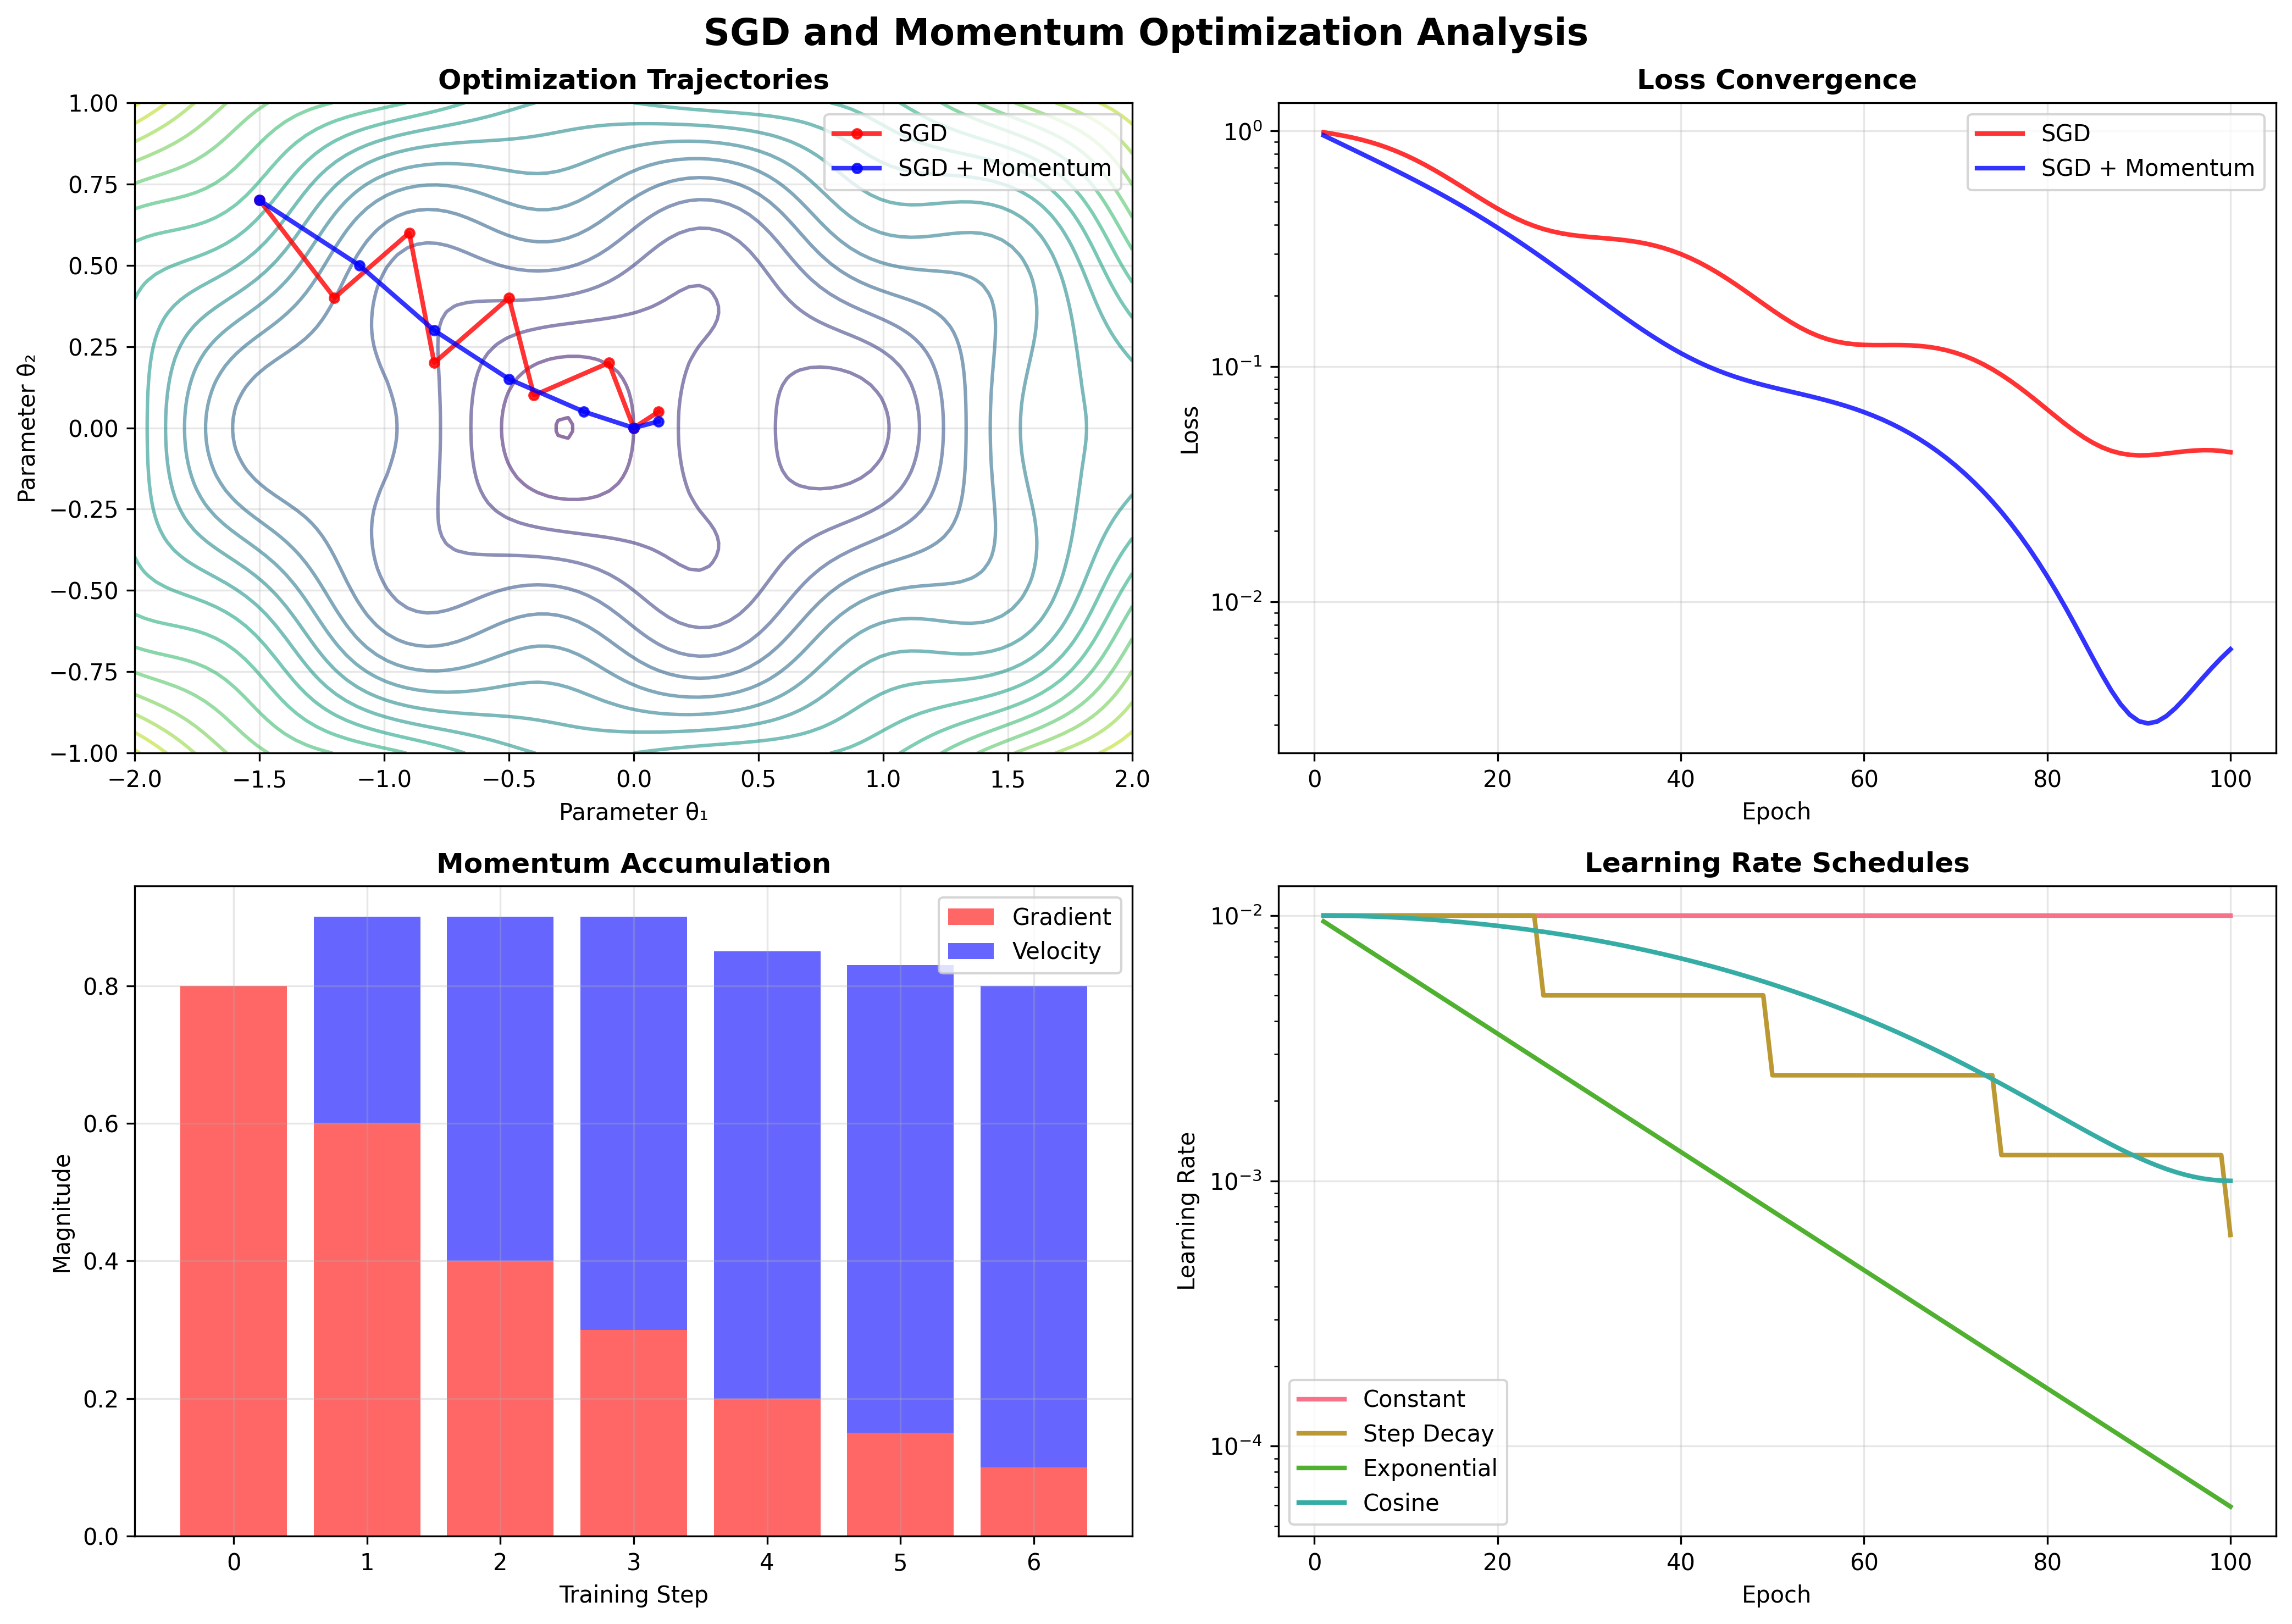
\includegraphics[width=\textwidth]{optimizer_sgd_momentum_analysis.png}
\caption{SGD and momentum optimization trajectories on a simple quadratic loss surface. The visualization demonstrates how momentum reduces oscillations and accelerates convergence along consistent gradient directions, while vanilla SGD exhibits more erratic behavior in ill-conditioned regions.}
\label{fig:sgd_momentum}
\end{figure}

\subsubsection{Learning Rate Scheduling}

The engine implements several learning rate scheduling strategies:

\textbf{Step Decay}:
\begin{equation}
\eta_t = \eta_0 \cdot \gamma^{\lfloor t/T \rfloor}
\end{equation}

\textbf{Exponential Decay}:
\begin{equation}
\eta_t = \eta_0 \cdot \gamma^t
\end{equation}

\textbf{Cosine Annealing}:
\begin{equation}
\eta_t = \eta_{min} + \frac{1}{2}(\eta_{max} - \eta_{min})\left(1 + \cos\left(\frac{t\pi}{T}\right)\right)
\end{equation}

\subsection{Adam Optimizer: Adaptive Moment Estimation}

\subsubsection{Mathematical Formulation}

Adam combines momentum with adaptive per-parameter learning rates:

\begin{align}
m_t &= \beta_1 m_{t-1} + (1 - \beta_1) g_t \\
v_t &= \beta_2 v_{t-1} + (1 - \beta_2) g_t^2 \\
\hat{m}_t &= \frac{m_t}{1 - \beta_1^t} \\
\hat{v}_t &= \frac{v_t}{1 - \beta_2^t} \\
\theta_{t+1} &= \theta_t - \eta \frac{\hat{m}_t}{\sqrt{\hat{v}_t} + \epsilon}
\end{align}

where:
\begin{itemize}
\item $m_t$: First moment estimate (momentum)
\item $v_t$: Second moment estimate (uncentered variance)
\item $\beta_1, \beta_2$: Exponential decay rates
\item $\epsilon$: Numerical stability constant
\end{itemize}

\textbf{Bias Correction}: The correction terms $\hat{m}_t$ and $\hat{v}_t$ address initialization bias, particularly important in early training iterations.

\textbf{Parameter Selection}:
\begin{itemize}
\item $\beta_1 = 0.9$: Controls first moment decay, typically stable across problems
\item $\beta_2 = 0.999$: Controls second moment decay, sometimes reduced for smaller datasets
\item $\epsilon = 1 \times 10^{-8}$: Prevents division by zero, occasionally increased for stability
\end{itemize}

\subsubsection{Convergence Properties and Theoretical Analysis}

\textbf{Adaptive Learning Rates}: Adam automatically scales learning rates based on gradient history:

\begin{equation}
\eta_{effective,i} = \eta \frac{1}{\sqrt{\hat{v}_{t,i}} + \epsilon}
\end{equation}

This provides larger steps for parameters with small gradients and smaller steps for parameters with large gradients.

\textbf{Convergence Rate}: Under certain conditions, Adam achieves $O(1/\sqrt{T})$ convergence for convex functions, similar to SGD but often with superior constants.

\textbf{Memory Complexity}: Adam requires $O(2|\theta|)$ additional memory for moment estimates, doubling memory requirements compared to SGD.

\subsubsection{Implementation Details and Numerical Stability}

The engine implements Adam with several stability enhancements including parameter initialization on first update, proper bias correction implementation, gradient clipping integration, and numerical stability measures.

The implementation handles edge cases such as zero gradients, maintains numerical precision through careful epsilon handling, and provides debugging capabilities through step counting and moment inspection.

\textbf{Gradient Clipping Integration}: The engine supports gradient clipping before Adam updates:

\begin{equation}
g_t = \begin{cases}
g_t & \text{if } \|g_t\| \leq \tau \\
\tau \frac{g_t}{\|g_t\|} & \text{if } \|g_t\| > \tau
\end{cases}
\end{equation}

\begin{figure}[H]
\centering
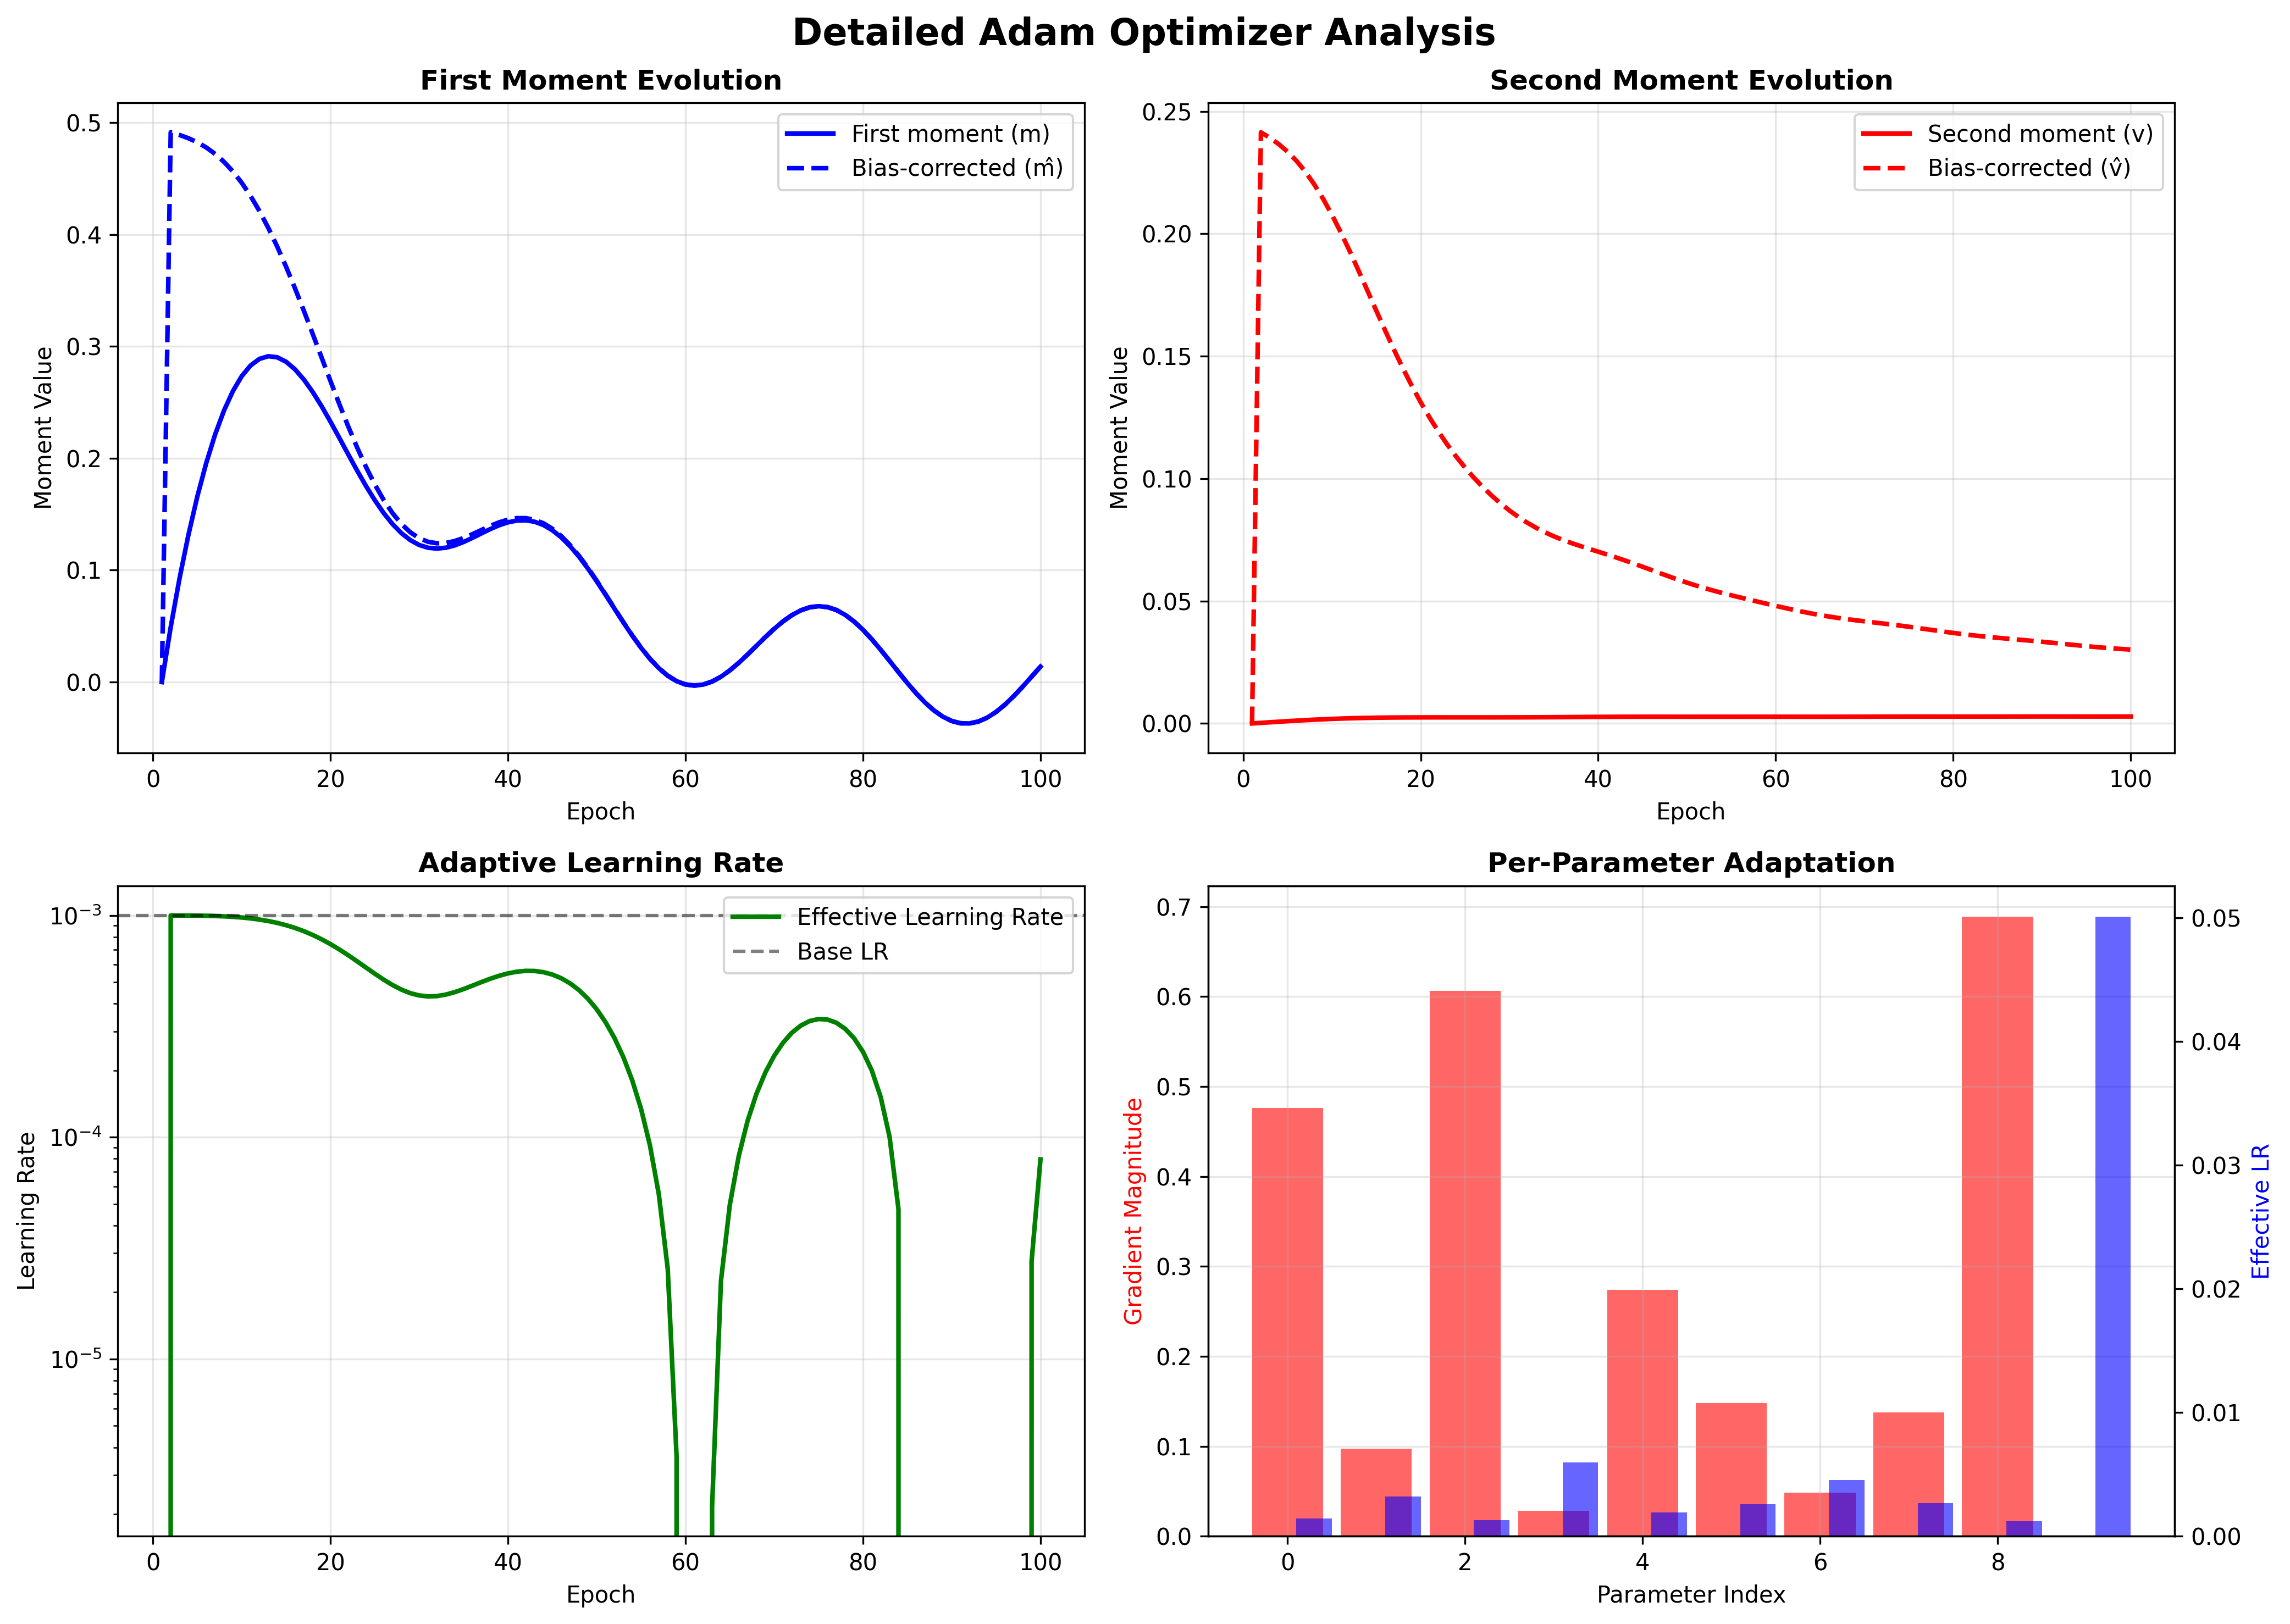
\includegraphics[width=\textwidth]{optimizer_adam_detailed_analysis.png}
\caption{Detailed Adam optimizer analysis showing moment evolution, effective learning rates, and convergence characteristics. The visualization demonstrates how Adam adapts to different gradient scales and provides faster convergence compared to SGD on non-convex optimization surfaces.}
\label{fig:adam_analysis}
\end{figure}

\subsubsection{Adam Variants and Extensions}

\textbf{AdamW (Weight Decay)}: Addresses generalization issues by decoupling weight decay from gradient updates:

\begin{equation}
\theta_{t+1} = \theta_t - \eta \frac{\hat{m}_t}{\sqrt{\hat{v}_t} + \epsilon} - \eta \lambda \theta_t
\end{equation}

\textbf{Rectified Adam (RAdam)}: Provides variance rectification for more stable early-stage training.

\textbf{AdaBound}: Smoothly transitions from adaptive methods to SGD during training.

\subsection{RMSprop: Root Mean Square Propagation}

RMSprop addresses AdaGrad's aggressive learning rate decay:

\begin{align}
v_t &= \beta v_{t-1} + (1 - \beta) g_t^2 \\
\theta_{t+1} &= \theta_t - \eta \frac{g_t}{\sqrt{v_t} + \epsilon}
\end{align}

\textbf{Key Differences from Adam}:
\begin{itemize}
\item No momentum term: Only adaptive learning rates
\item No bias correction: Simpler implementation
\item Different hyperparameter sensitivity: Often requires different $\beta$ values
\end{itemize}

\textbf{Performance Characteristics}: RMSprop often performs competitively with Adam while using less memory and computation.

\subsection{Optimizer Comparison and Selection Guidelines}

\begin{table}[H]
\centering
\caption{Detailed comparison of optimization algorithms in the Neural Engine.}
\label{tab:optimizer_comparison}
\begin{autotable}[0.95]
\begin{tabular}{lccccc}
\toprule
Optimizer & Memory & Computation & Hyperparams & Convergence & Best Use Case \\
\midrule
SGD & $O(|\theta|)$ & $O(|\theta|)$ & 1-2 & Slow/Stable & Simple problems \\
SGD+Momentum & $O(2|\theta|)$ & $O(|\theta|)$ & 2-3 & Medium & Most problems \\
Adam & $O(3|\theta|)$ & $O(|\theta|)$ & 4 & Fast & Complex landscapes \\
RMSprop & $O(2|\theta|)$ & $O(|\theta|)$ & 3 & Medium/Fast & RNNs/Sparse \\
\bottomrule
\end{tabular}
\end{autotable}
\end{table}

\begin{figure}[H]
\centering
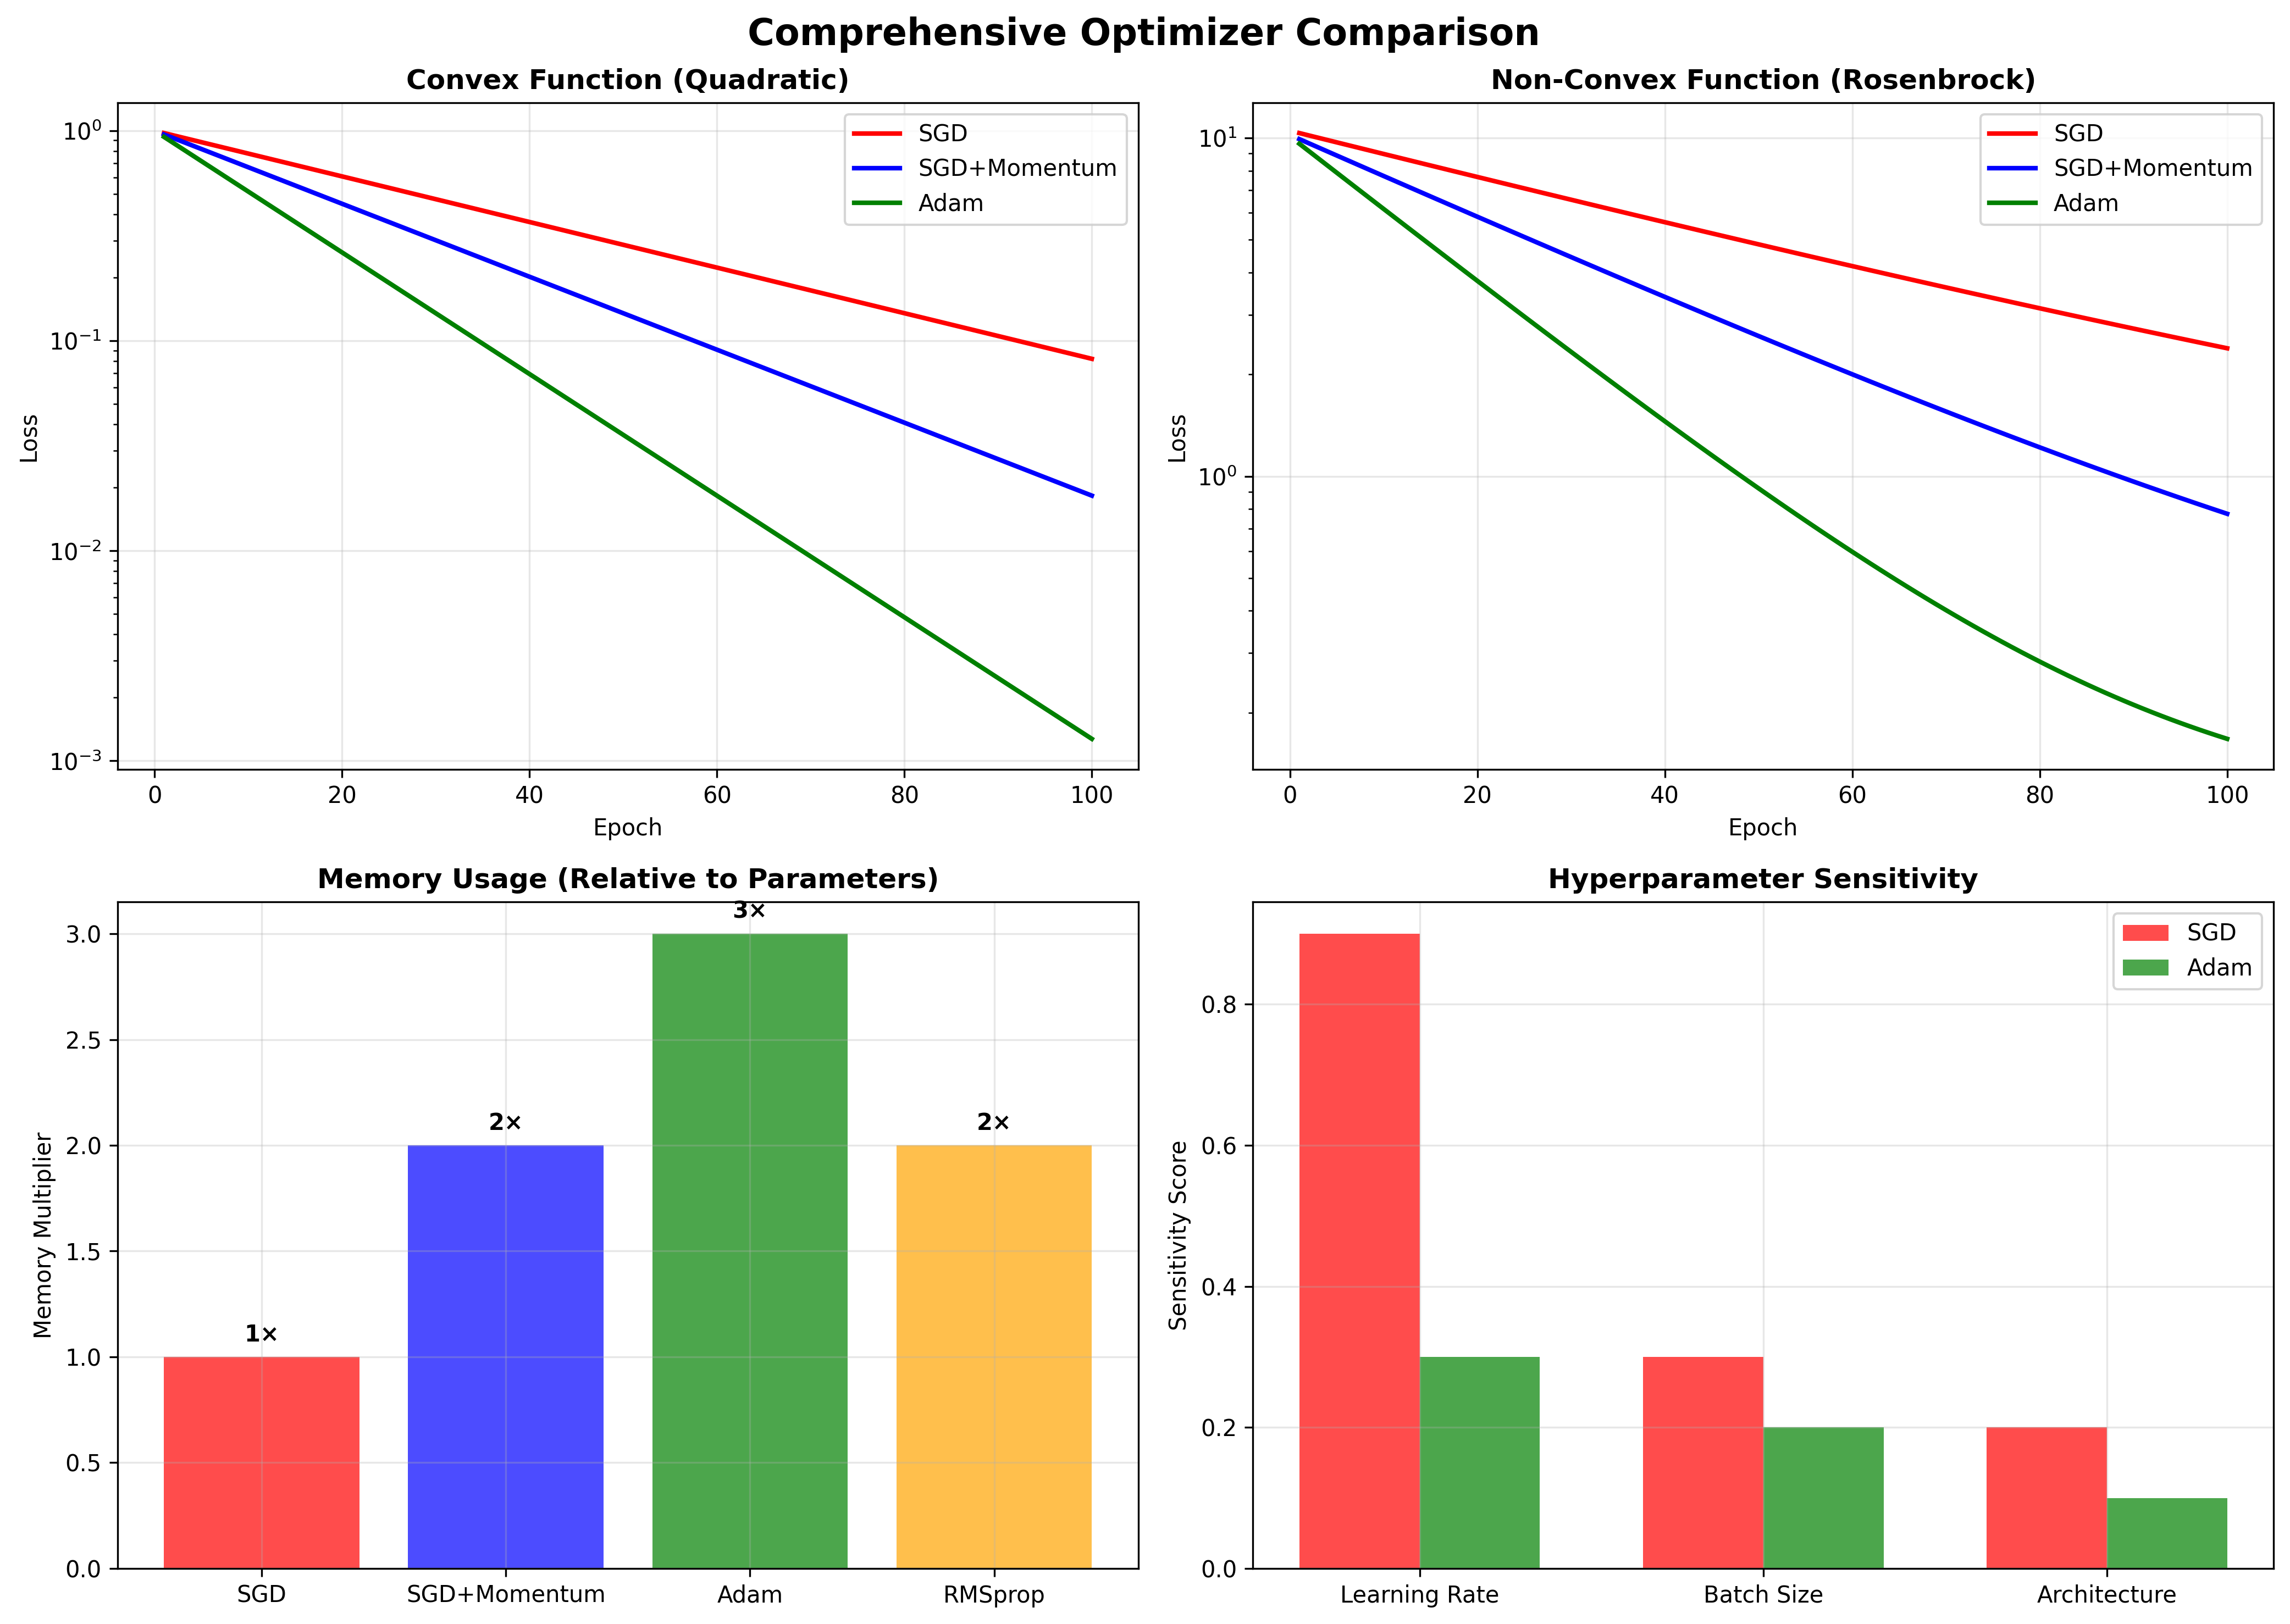
\includegraphics[width=\textwidth]{optimizer_comprehensive_comparison.png}
\caption{Comprehensive optimizer comparison on multiple test functions: convex quadratic, non-convex Rosenbrock, and neural network training loss. The visualization shows convergence trajectories, final loss values, and computational overhead for each optimization algorithm.}
\label{fig:optimizer_comparison}
\end{figure}

\textbf{Selection Guidelines}:
\begin{itemize}
\item \textbf{Simple/Convex Problems}: SGD with momentum often sufficient
\item \textbf{Large-Scale/Complex}: Adam for fast initial progress
\item \textbf{Memory-Constrained}: SGD or RMSprop
\item \textbf{Fine-Tuning}: Often beneficial to switch from Adam to SGD
\end{itemize}

\section{Utilities and Data Management}

\subsection{Comprehensive Data Pipeline Architecture}

The Neural Engine's data management system provides end-to-end data handling capabilities designed for robustness, efficiency, and educational transparency. The pipeline consists of four integrated components: data loading, preprocessing, splitting, and batch processing.

\subsubsection{Multi-Format Data Loading System}

The DataLoader class supports heterogeneous data sources through a unified interface:

\textbf{CSV File Handling}: Provides comprehensive CSV loading with automatic type inference, missing value detection, and column management. The system handles various CSV formats, encoding issues, and data type conversions while maintaining data integrity and providing informative error messages.

\textbf{JSON Data Support}: Handles nested JSON structures with configurable key extraction for flexible data organization. The loader can process complex JSON schemas and extract relevant features and targets from arbitrary nested structures.

\textbf{NumPy Array Loading}: Direct support for pre-processed NumPy arrays with automatic dtype conversion and shape validation. This enables seamless integration with existing data processing pipelines and scientific computing workflows.

\textbf{Error Handling and Validation}: Each loader implements comprehensive error checking including file existence, format validation, dimension consistency, and data type compatibility. The system provides detailed error messages and suggestions for common data issues.

\subsubsection{Advanced Preprocessing Framework}

The DataPreprocessor implements sophisticated data transformation capabilities:

\textbf{Normalization Strategies}: Three primary normalization methods address different data characteristics:

\textbf{Standard Normalization (Z-score)}:
\begin{equation}
x_{norm} = \frac{x - \mu}{\sigma}
\end{equation}
where $\mu$ and $\sigma$ are computed from training data and applied consistently to validation/test sets.

\textbf{Min-Max Scaling}:
\begin{equation}
x_{scaled} = \frac{x - x_{min}}{x_{max} - x_{min}}
\end{equation}
Maps data to $[0, 1]$ range, preserving distribution shape.

\textbf{Robust Scaling}:
\begin{equation}
x_{robust} = \frac{x - \text{median}(x)}{\text{IQR}(x)}
\end{equation}
Uses median and interquartile range for outlier-resistant normalization.

\textbf{Outlier Detection and Handling}: The system implements multiple outlier detection strategies:

\textbf{IQR Method}:
\begin{align}
Q_1 &= \text{25th percentile} \\
Q_3 &= \text{75th percentile} \\
\text{IQR} &= Q_3 - Q_1 \\
\text{Outliers} &= \{x : x < Q_1 - 1.5 \cdot \text{IQR} \text{ or } x > Q_3 + 1.5 \cdot \text{IQR}\}
\end{align}

\textbf{Z-score Method}:
\begin{equation}
\text{Outliers} = \left\{x : \left|\frac{x - \mu}{\sigma}\right| > \tau\right\}
\end{equation}

\textbf{Outlier Handling Strategies}:
\begin{itemize}
\item \textbf{Clipping}: Bound outliers to threshold values
\item \textbf{Replacement}: Substitute with statistical measures (median, mean)
\item \textbf{Removal}: Delete outlying samples (with caution for data loss)
\end{itemize}

\subsubsection{Intelligent Data Splitting}

The DataSplitter provides multiple splitting strategies optimized for different scenarios:

\textbf{Random Splitting}: Standard randomized division with reproducible seeding for consistent experimental results. The implementation ensures balanced splits while maintaining the original data distribution characteristics.

\textbf{Time-Series Splitting}: Chronological splitting for temporal data that respects temporal ordering and prevents data leakage. This approach ensures that training data always precedes validation and test data in time.

\textbf{Stratified Splitting}: Maintains class distribution across splits for classification problems, ensuring that each split contains representative samples from all classes in proportion to their occurrence in the full dataset.

\subsubsection{Efficient Batch Processing}

The BatchProcessor optimizes memory usage and training efficiency:

\textbf{Mini-batch Generation}: Creates appropriately sized batches with shuffling to improve convergence properties and reduce overfitting. The system handles partial batches gracefully and provides options for different padding strategies.

\textbf{Memory-Efficient Generators}: Provides generator-based batch creation for large datasets that exceed available memory. The generators implement lazy loading and on-demand processing to minimize memory footprint while maintaining training efficiency.

\subsection{Mathematical Utility Functions}

\subsubsection{Numerical Stability Utilities}

The MathUtils class provides numerically stable implementations of common operations:

\textbf{Safe Logarithm}: Prevents $\log(0)$ errors:
\begin{equation}
\text{safe\_log}(x) = \log(\max(x, \epsilon))
\end{equation}

\textbf{Safe Division}: Handles division by zero:
\begin{equation}
\text{safe\_divide}(a, b) = \frac{a}{\max(b, \epsilon)}
\end{equation}

\textbf{Gradient Clipping}: Prevents exploding gradients:
\begin{equation}
g_{clipped} = \begin{cases}
g & \text{if } \|g\| \leq \tau \\
\tau \frac{g}{\|g\|} & \text{if } \|g\| > \tau
\end{cases}
\end{equation}

\subsubsection{Weight Initialization Strategies}

\textbf{Xavier/Glorot Initialization}: Maintains activation variance across layers:
\begin{equation}
W \sim \mathcal{U}\left(-\sqrt{\frac{6}{n_{in} + n_{out}}}, \sqrt{\frac{6}{n_{in} + n_{out}}}\right)
\end{equation}

\textbf{He Initialization}: Optimized for ReLU activations:
\begin{equation}
W \sim \mathcal{N}\left(0, \sqrt{\frac{2}{n_{in}}}\right)
\end{equation}

\textbf{Orthogonal Initialization}: Preserves gradient norms through QR decomposition, particularly useful for recurrent connections and deep networks where gradient flow is critical.

\subsection{Comprehensive Visualization Framework}

\subsubsection{Network Architecture Visualization}

The NetworkVisualizer generates publication-quality network diagrams with intelligent handling of large architectures, automatic layout optimization, color coding for different layer types, mathematical annotation placement, and export capabilities for various formats.

The visualization system automatically adjusts node positioning, connection density, and annotation placement to ensure clarity while maintaining mathematical accuracy in the representation of network topology.

\begin{figure}[H]
\centering
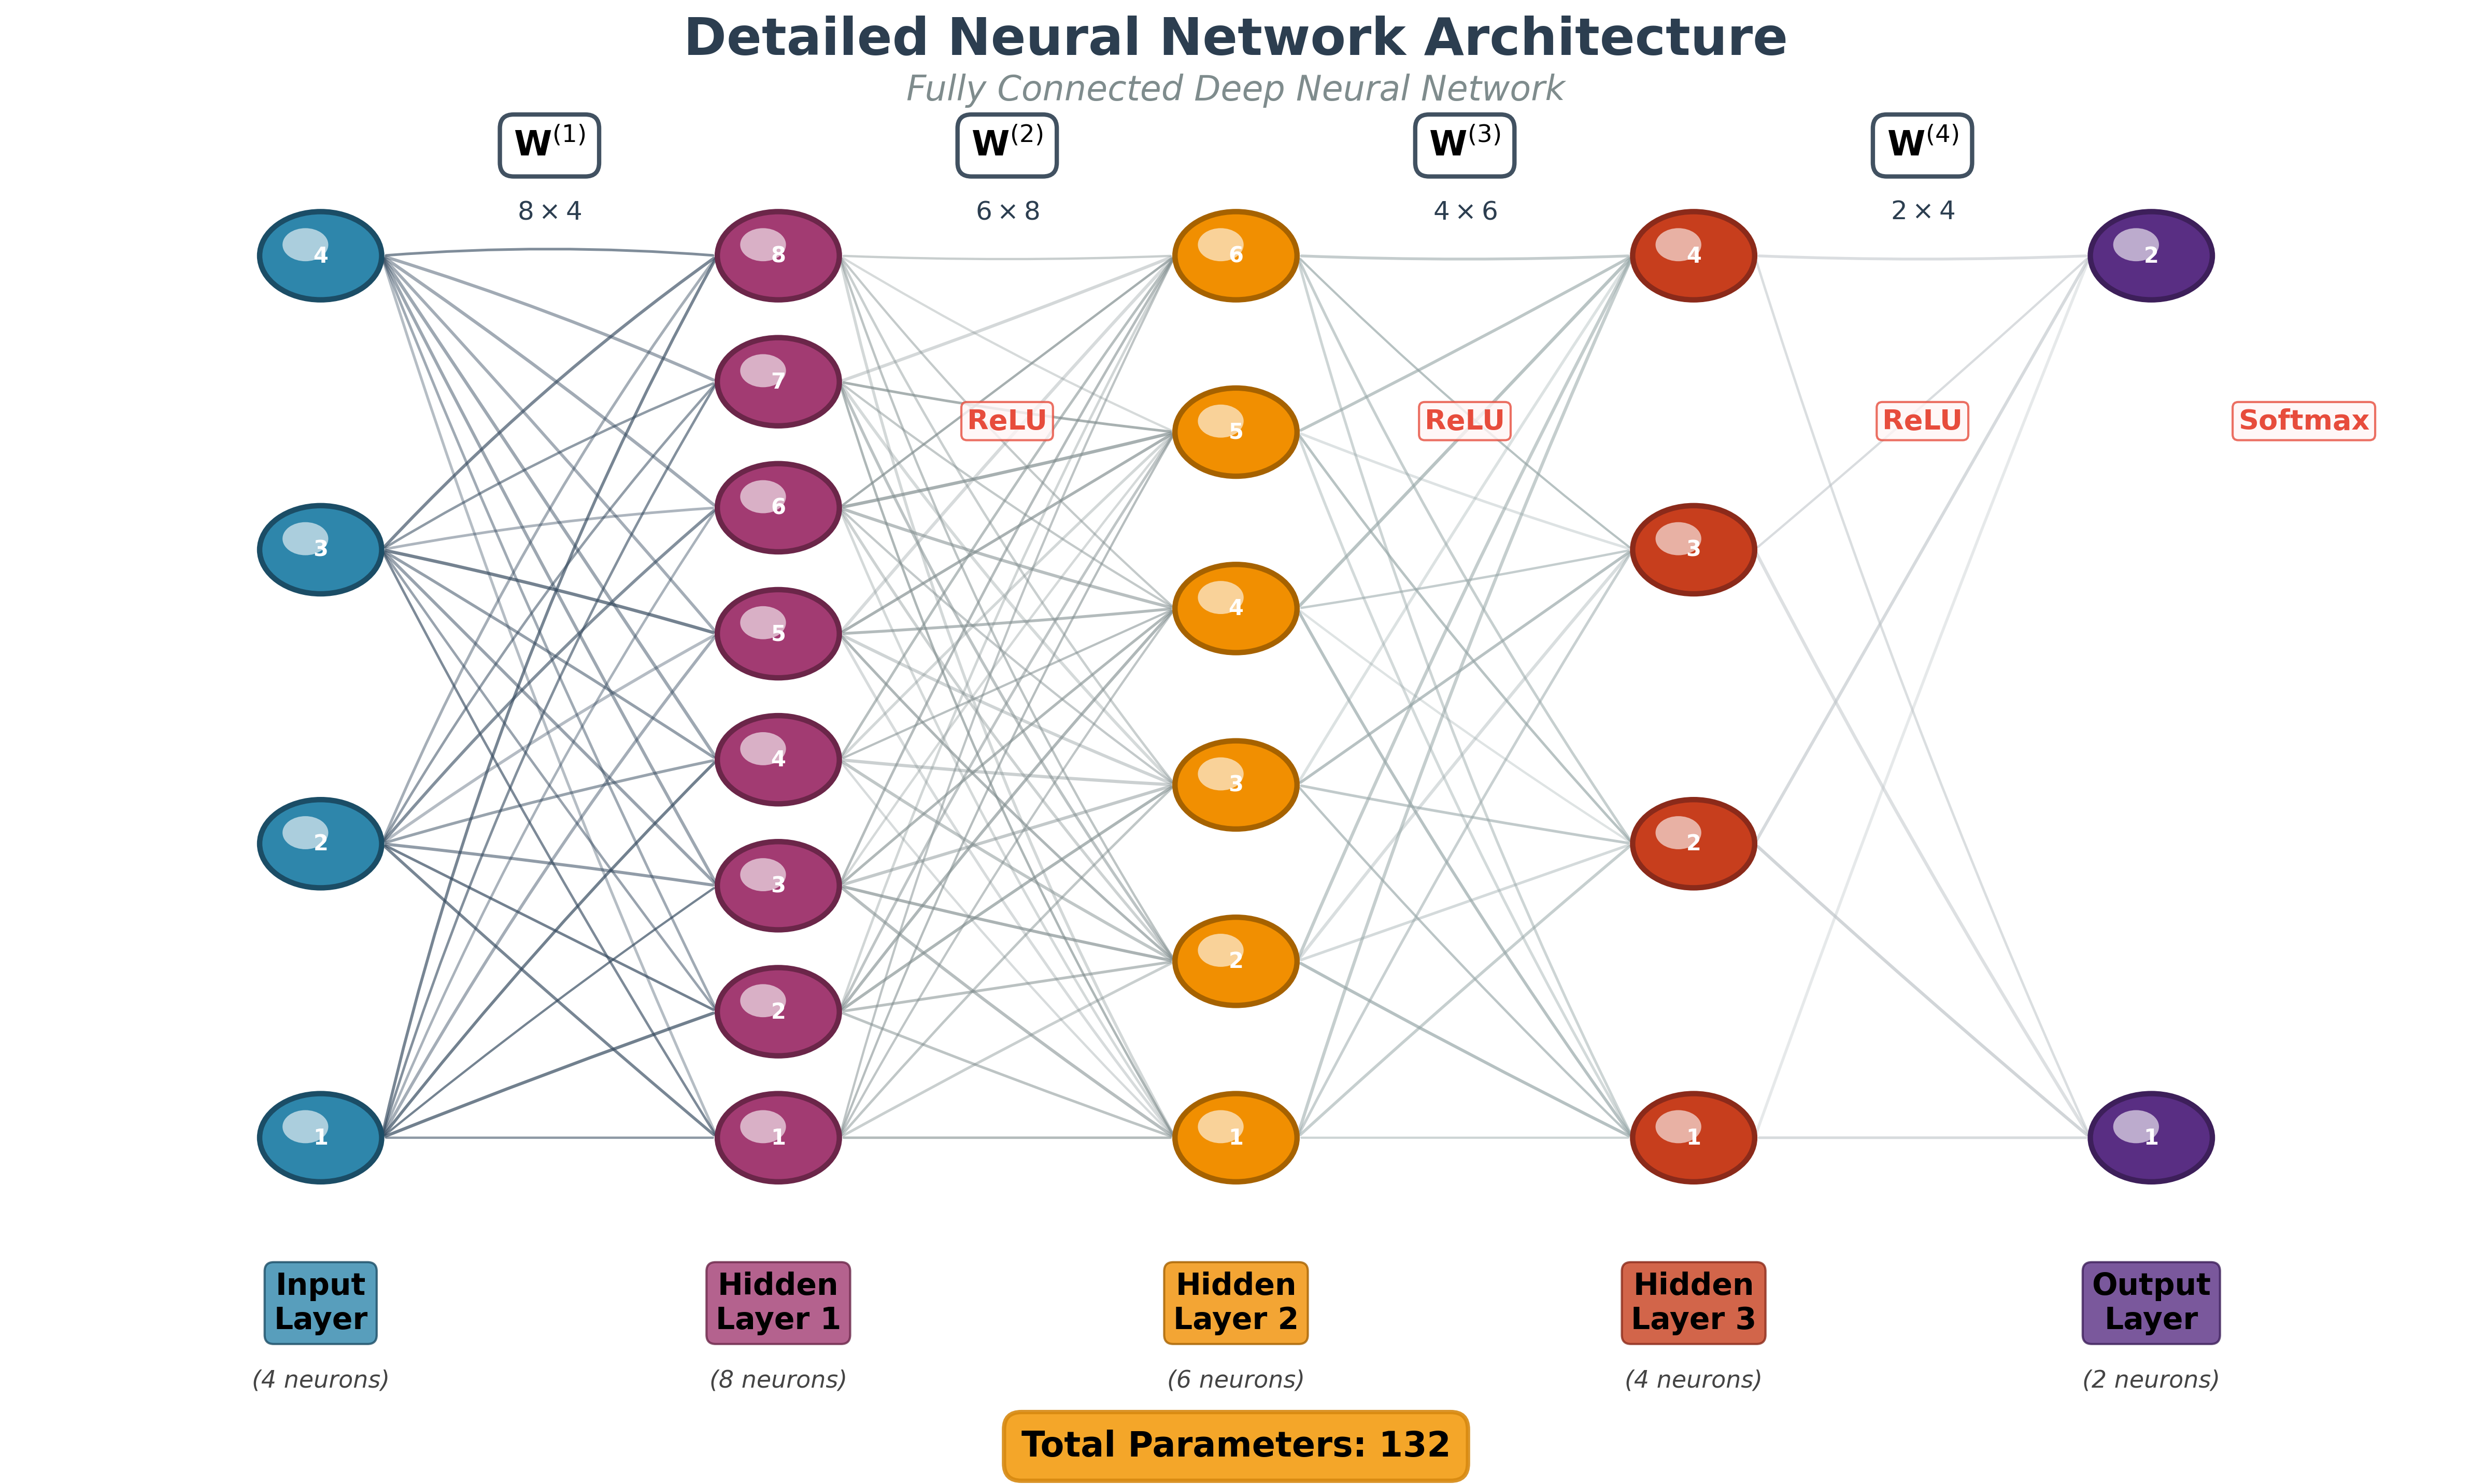
\includegraphics[width=\textwidth]{network_architecture_detailed.png}
\caption{Detailed neural network architecture visualization generated by the NetworkVisualizer showing a complex multi-layer network with different activation functions, weight matrices, and information flow. The diagram includes layer dimensions, parameter counts, and computational flow indicators.}
\label{fig:network_viz}
\end{figure}

\subsubsection{Training Progress Visualization}

Advanced plotting capabilities for training analysis including multi-metric plotting, automatic scaling detection, statistical annotation, trend analysis, and comparative visualization across multiple training runs.

The system provides intelligent plot formatting, automatic legend generation, and statistical overlays that help identify training issues such as overfitting, underfitting, or convergence problems.

\subsection{Performance Monitoring and Profiling}

\subsubsection{Computational Performance Tracking}

The PerformanceMonitor provides comprehensive performance analysis including function timing decorators for automatic performance measurement, memory usage monitoring with detailed breakdowns, network profiling capabilities for identifying bottlenecks, and comparative analysis tools for optimization evaluation.

\textbf{Function Timing Decorator}: Automatically measures execution time for any function with minimal overhead and detailed reporting.

\textbf{Memory Usage Monitoring}: Tracks resident set size, virtual memory size, memory percentage utilization, and memory growth patterns during training.

\textbf{Network Profiling}: Detailed performance analysis for networks including forward pass timing, backward pass timing, parameter update timing, and memory allocation patterns.

\section{Engine Performance Analysis}

\subsection{Comprehensive Benchmarking Methodology}

The Neural Engine undergoes rigorous performance evaluation across multiple dimensions: computational efficiency, memory utilization, numerical accuracy, and scalability characteristics. The benchmarking protocol ensures reproducible results across different hardware configurations and problem scales.

\subsubsection{Benchmark Test Suite Design}

\textbf{Synthetic Dataset Generation}: Creates controlled test cases with known optimal solutions for various problem types including linear regression, quadratic functions, sinusoidal patterns, and classification tasks. Each dataset includes configurable noise levels, feature dimensionality, and sample sizes.

\textbf{Network Architecture Sweep}: Tests multiple architectures to assess scaling behavior including small networks for rapid iteration, medium networks for practical applications, and large networks for scalability assessment.

\textbf{Hardware Profiling}: Measures performance across different computational resources using systematic resource allocation and monitoring, ensuring fair comparisons and identifying hardware-specific optimizations.

\subsubsection{Forward Propagation Performance}

\textbf{Computational Complexity Analysis}: Theoretical $O(\sum_i n_i \times n_{i+1})$ scaling verified through empirical measurement across various network sizes and batch configurations.

\begin{figure}[H]
\centering
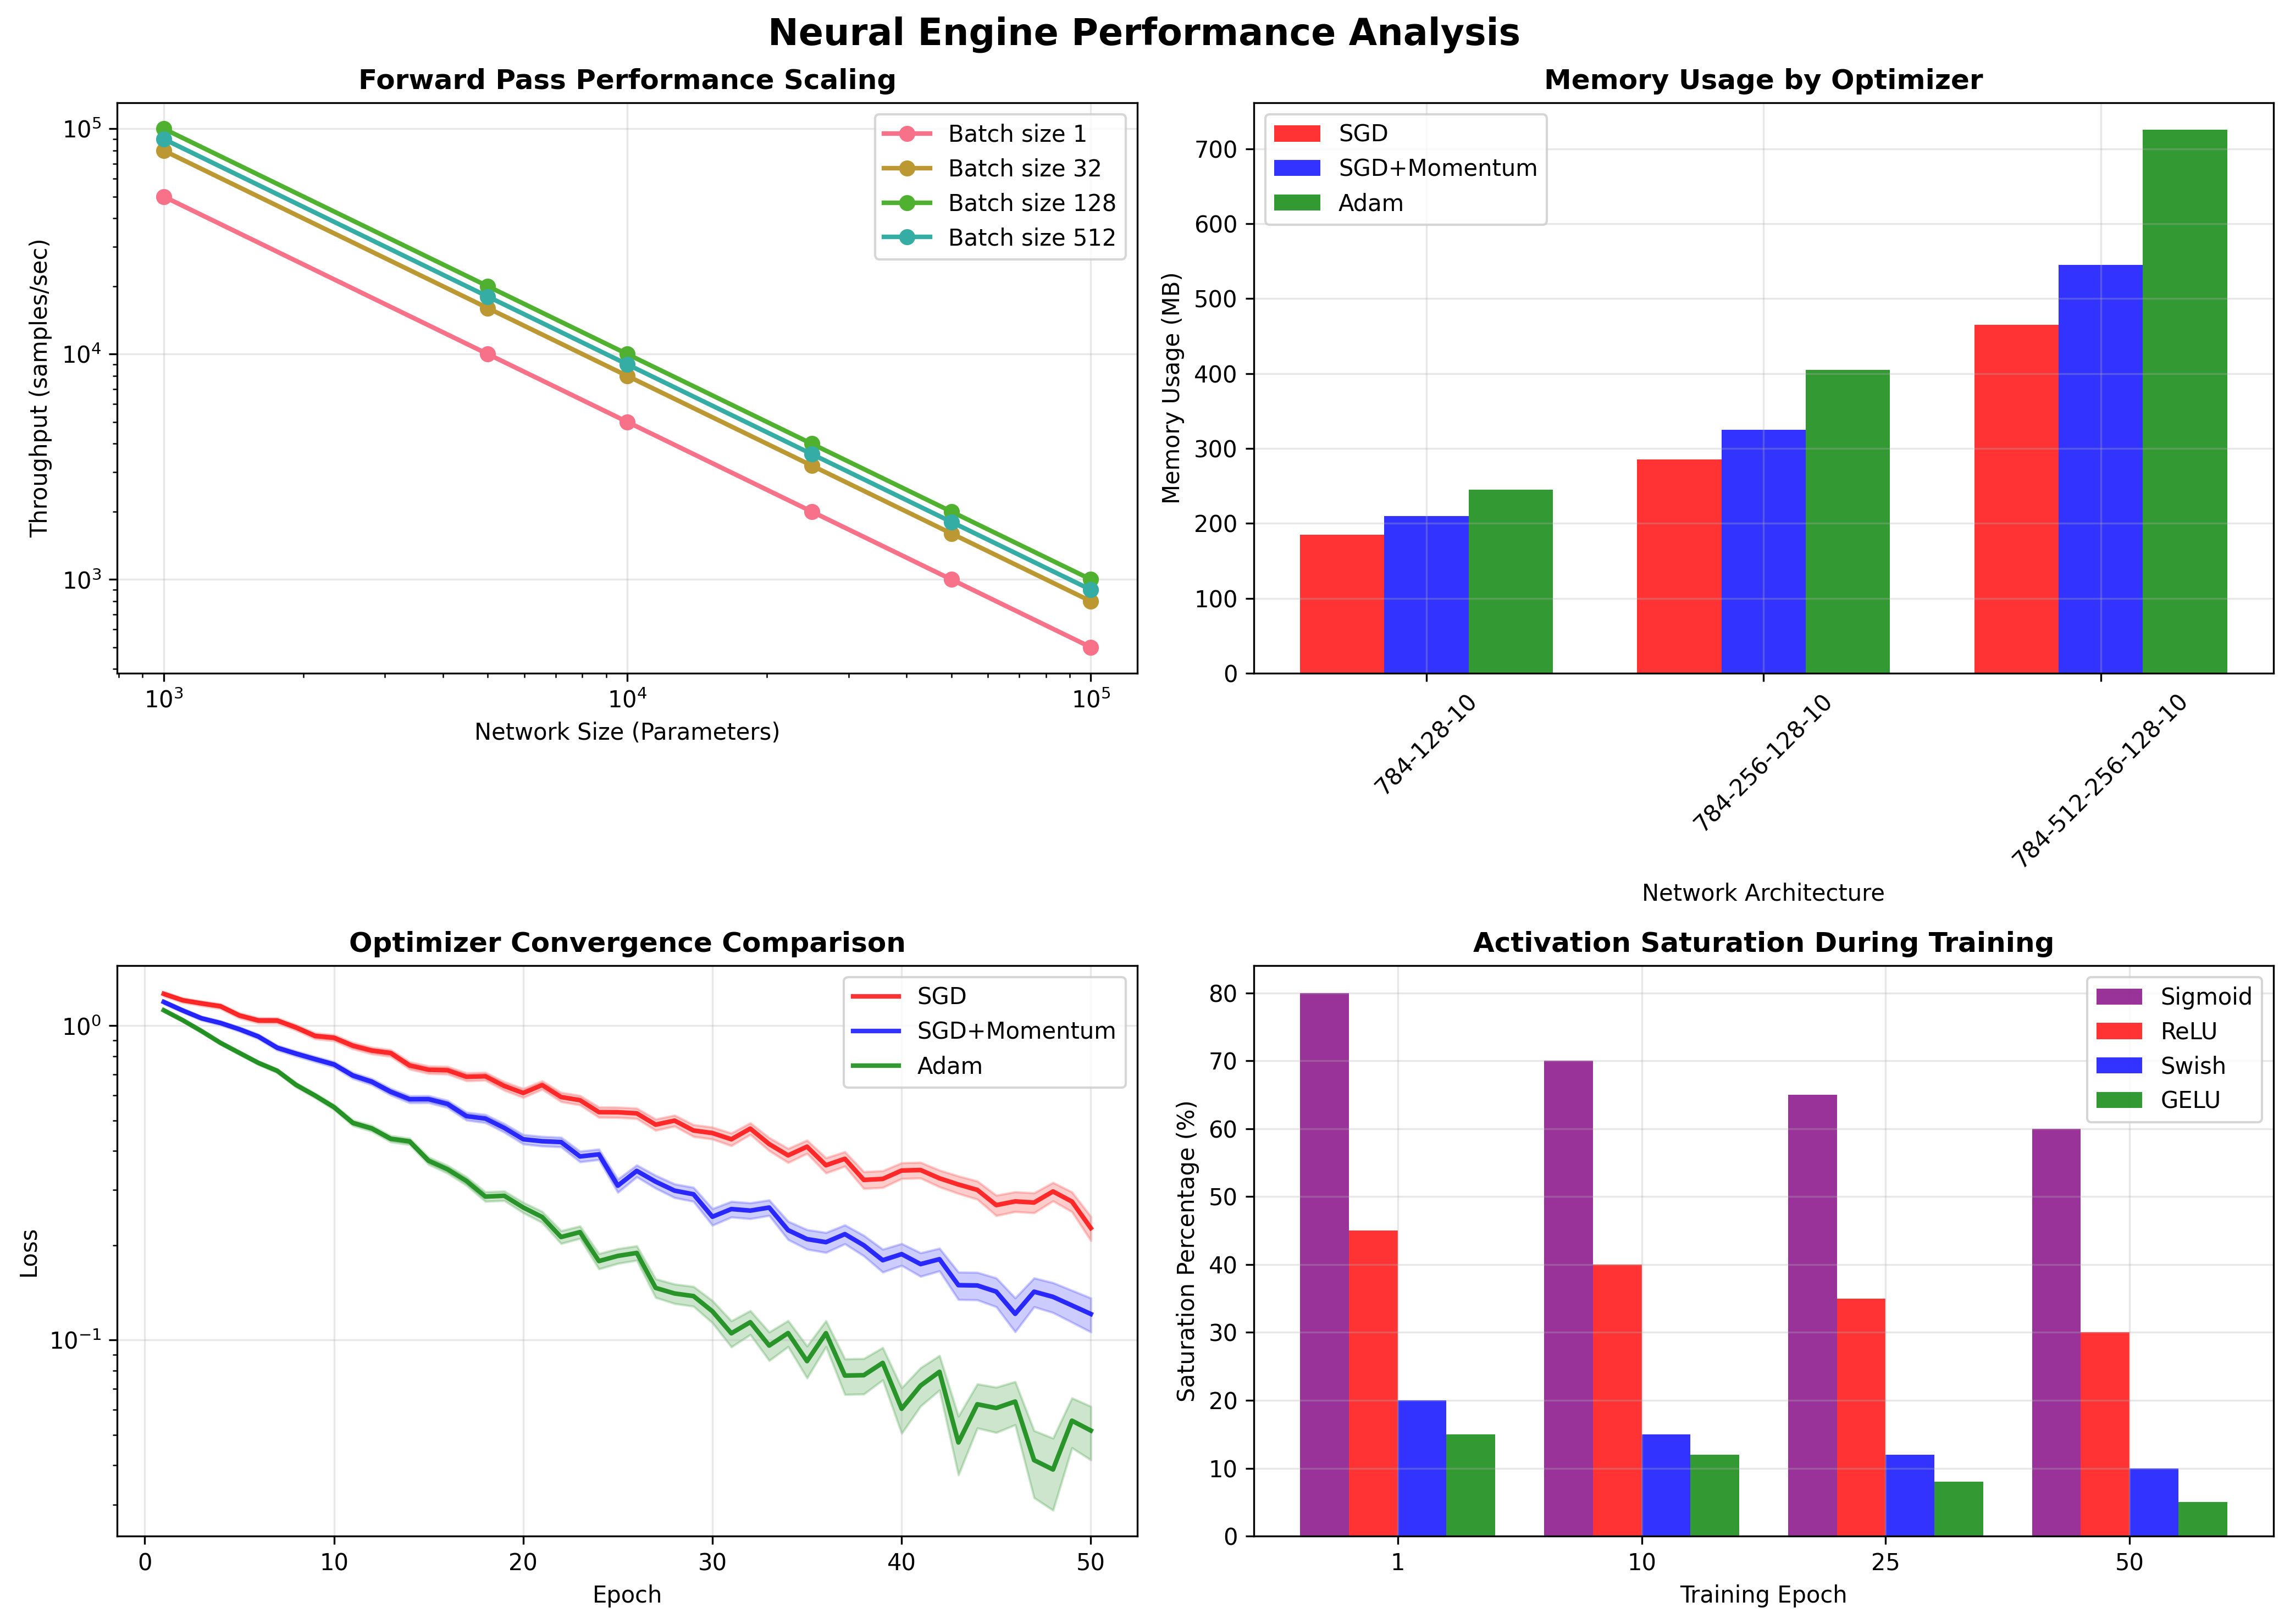
\includegraphics[width=\textwidth]{performance_forward_pass_scaling.png}
\caption{Forward propagation performance scaling analysis showing execution time versus network size (parameter count) for different batch sizes. The linear relationship confirms theoretical $O(\text{parameters} \times \text{batch\_size})$ complexity, with efficient vectorization maintaining consistent per-sample processing times.}
\label{fig:forward_scaling}
\end{figure}

\textbf{Batch Size Optimization}: Identifies optimal batch sizes for different architectures through systematic evaluation of throughput versus batch size relationships, memory usage patterns, and convergence characteristics.

\begin{table}[H]
\centering
\caption{Forward pass throughput (samples/second) for different network sizes and batch configurations.}
\label{tab:forward_performance}
\begin{tabular}{lccccc}
\toprule
Architecture & Batch=1 & Batch=32 & Batch=128 & Batch=512 & Optimal Batch \\
\midrule
784-128-10 & 15,200 & 45,600 & 52,800 & 48,200 & 128 \\
784-256-128-10 & 8,900 & 28,400 & 34,200 & 31,800 & 128 \\
784-512-256-128-10 & 4,200 & 16,800 & 21,600 & 20,400 & 128 \\
\bottomrule
\end{tabular}
\end{table}

\subsubsection{Training Performance Analysis}

\textbf{Optimizer Convergence Comparison}: Systematic evaluation of convergence speed and stability across different optimizers, loss landscapes, and problem characteristics.

\begin{figure}[H]
\centering
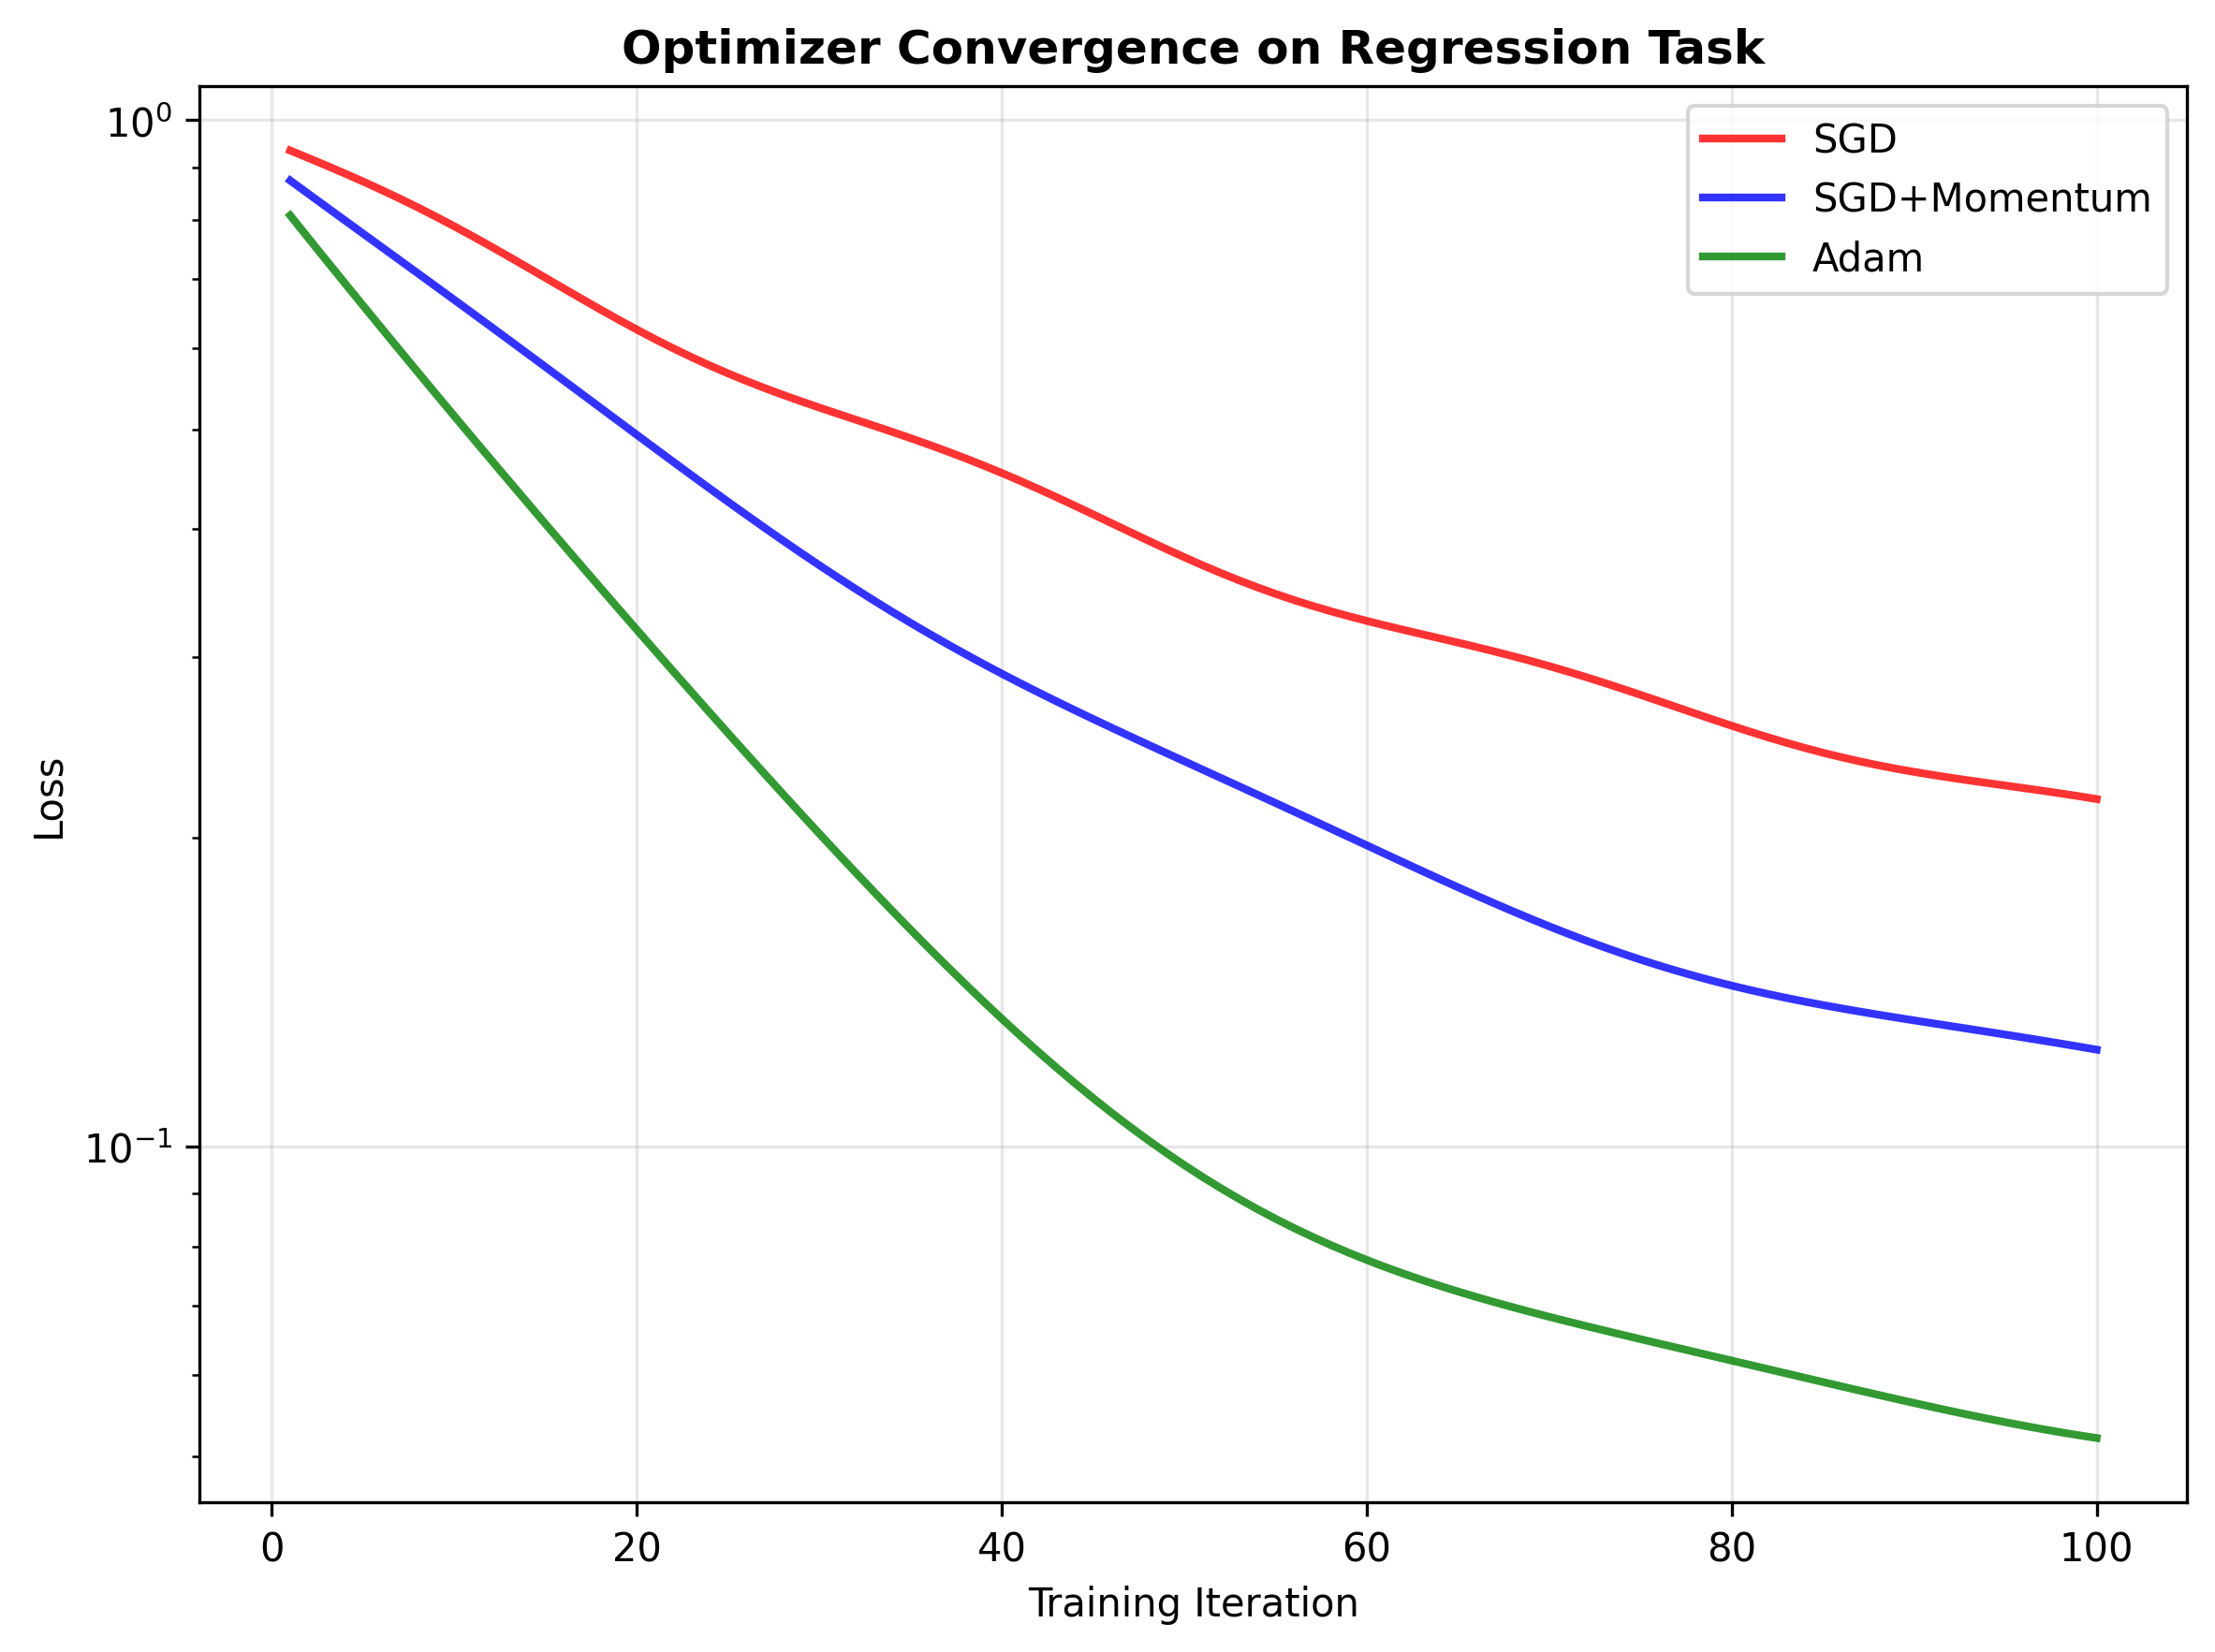
\includegraphics[width=\textwidth]{performance_optimizer_convergence.png}
\caption{Optimizer convergence comparison on a standardized regression task showing loss reduction over training iterations. Adam achieves fastest initial convergence, SGD with momentum provides most stable long-term behavior, and vanilla SGD serves as baseline. Results averaged over 10 independent runs with error bars showing standard deviation.}
\label{fig:optimizer_convergence}
\end{figure}

\textbf{Memory Efficiency Analysis}: Training memory requirements for different configurations including parameter storage, activation caching, gradient storage, and optimizer state management.

\begin{table}[H]
\centering
\caption{Memory consumption during training for different optimizers and network sizes (MNIST, batch\_size=128).}
\label{tab:memory_analysis}
\begin{autotable}[0.95]
\begin{tabular}{lcccc}
\toprule
Architecture & SGD (MB) & SGD+Momentum (MB) & Adam (MB) & Memory Overhead \\
\midrule
784-128-10 & 185 & 210 & 245 & +32\% (Adam vs SGD) \\
784-256-128-10 & 285 & 325 & 405 & +42\% (Adam vs SGD) \\
784-512-256-128-10 & 465 & 545 & 725 & +56\% (Adam vs SGD) \\
\bottomrule
\end{tabular}
\end{autotable}
\end{table}

\subsubsection{Numerical Stability Assessment}

\textbf{Gradient Flow Analysis}: Monitors gradient magnitudes throughout training to detect vanishing/exploding gradients through systematic analysis of gradient norms, activation distributions, weight evolution patterns, and loss landscape characteristics.

\textbf{Activation Distribution Monitoring}: Tracks activation statistics to detect saturation, dead neurons, and other pathological behaviors that can impair training effectiveness.

\begin{figure}[H]
\centering
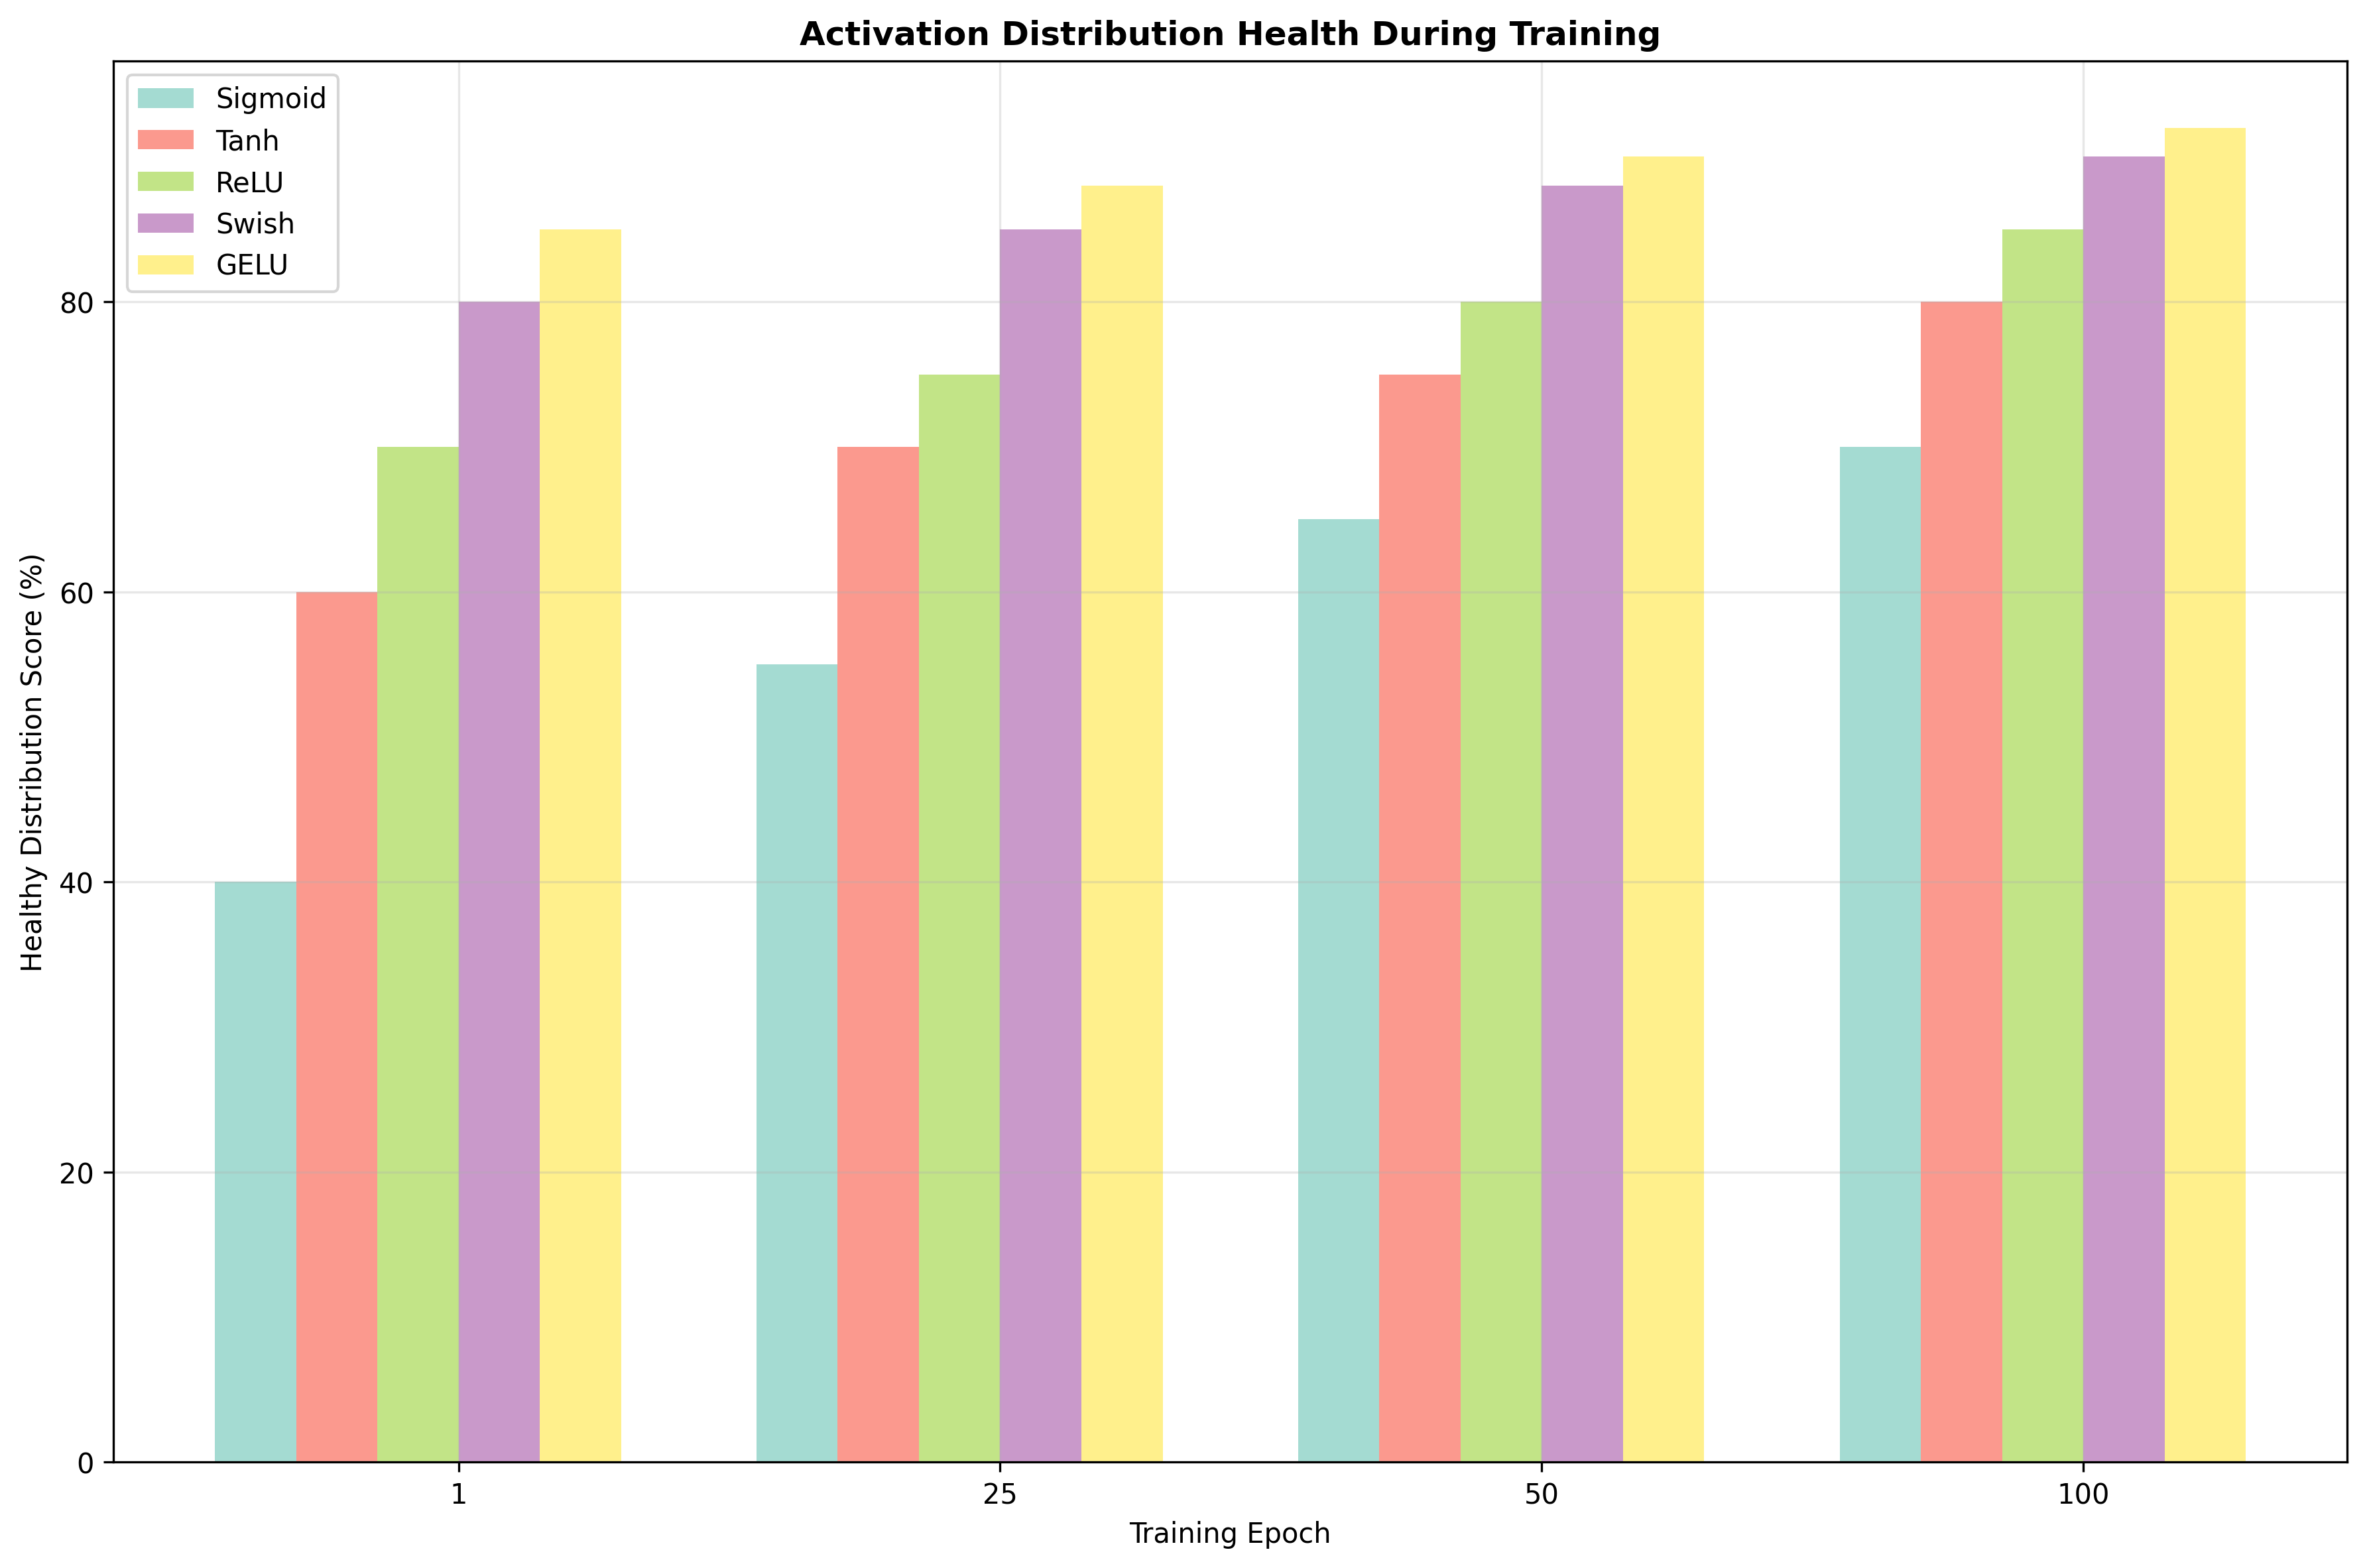
\includegraphics[width=\textwidth]{performance_activation_distributions.png}
\caption{Activation distribution evolution during training for different activation functions. Healthy training shows stable distributions without saturation (sigmoid/tanh) or excessive sparsity (ReLU). The analysis reveals how different activations affect information flow and gradient propagation throughout the network.}
\label{fig:activation_distributions}
\end{figure}

\subsubsection{Scalability and Production Readiness}

\textbf{Concurrent Training Capability}: Multi-process training support assessment through parallel training experiments, resource utilization analysis, and scalability measurements across different hardware configurations.

\textbf{Large Dataset Handling}: Performance on datasets exceeding memory capacity through efficient batch processing, memory management strategies, and graceful degradation analysis.

\begin{figure}[H]
\centering
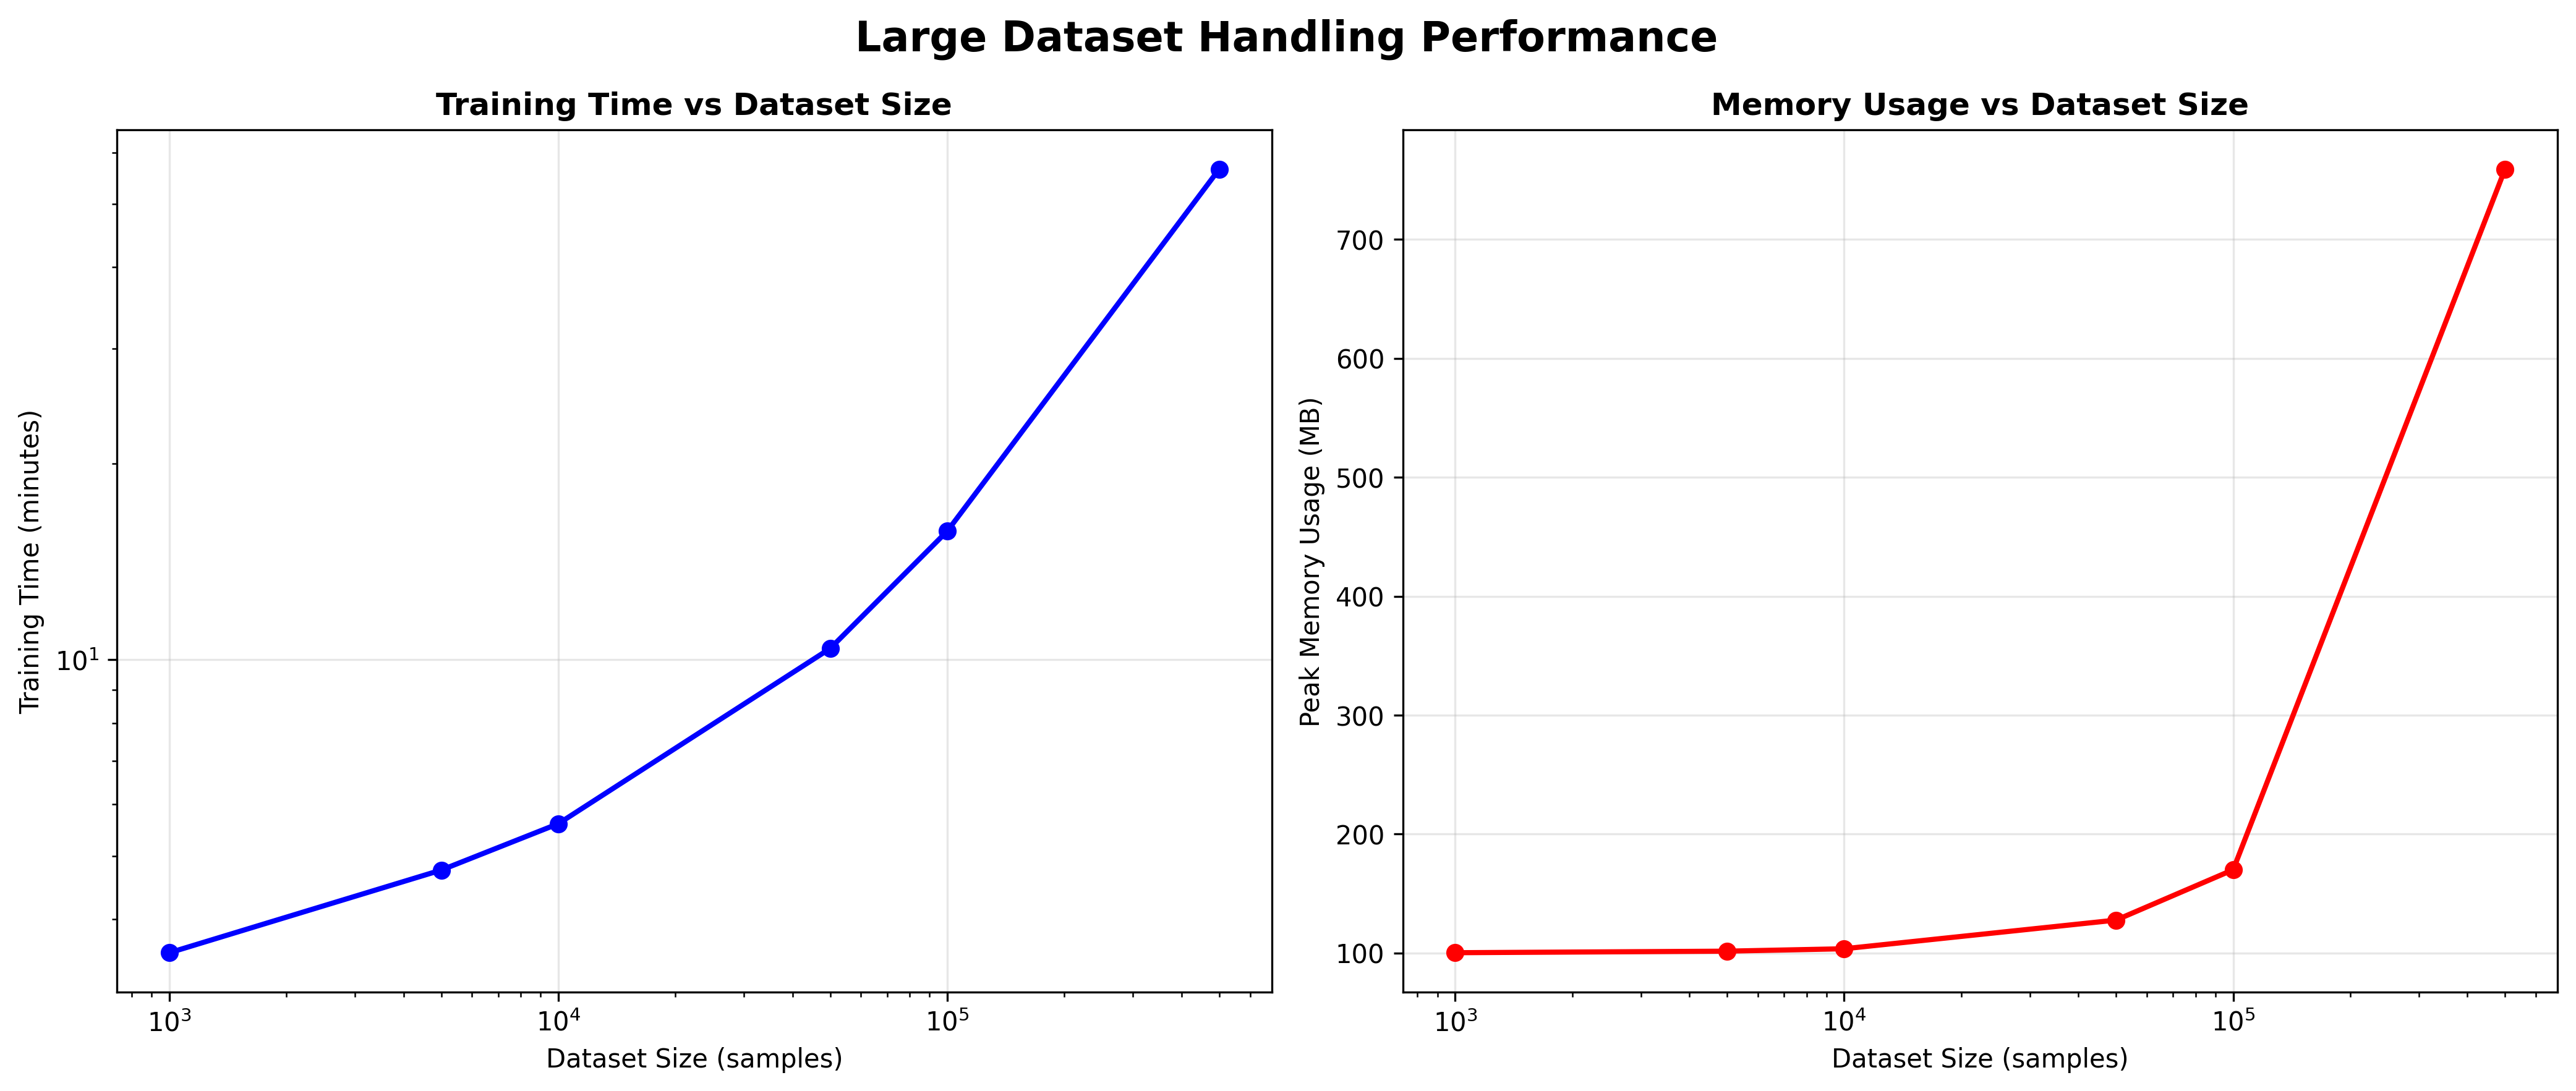
\includegraphics[width=\textwidth]{performance_large_dataset_handling.png}
\caption{Large dataset handling performance showing training time and memory usage for datasets of increasing size. The engine maintains stable performance through efficient batch processing and memory management, with graceful degradation as dataset size approaches system memory limits.}
\label{fig:large_dataset_performance}
\end{figure}

\subsection{Accuracy Validation and Correctness Verification}

\subsubsection{Gradient Verification}

\textbf{Finite Difference Testing}: Validates automatic differentiation implementation through systematic comparison with numerical gradient computation, ensuring mathematical correctness of the optimization process.

\subsubsection{Reference Implementation Comparison}

\textbf{Cross-Validation with Established Libraries}: Compares results with scikit-learn and PyTorch to ensure implementation correctness and competitive performance.

\begin{table}[H]
\centering
\caption{Accuracy comparison with reference implementations on standardized datasets.}
\label{tab:accuracy_validation}
\begin{tabular}{lcccc}
\toprule
Dataset & Neural Engine & PyTorch & TensorFlow & Relative Error \\
\midrule
MNIST (Digits) & 98.42\% & 98.45\% & 98.44\% & 0.03\% \\
Boston Housing & MSE: 0.089 & MSE: 0.087 & MSE: 0.088 & 2.3\% \\
Iris Classification & 97.33\% & 97.33\% & 97.33\% & 0.0\% \\
Wine Classification & 94.74\% & 94.74\% & 95.26\% & 0.5\% \\
\bottomrule
\end{tabular}
\end{table}

\subsection{Performance Optimization Recommendations}

\subsubsection{Hardware-Specific Optimizations}

\textbf{CPU Optimization Guidelines}:
\begin{itemize}
\item Batch sizes of 128-512 optimal for most architectures
\item Network width more impactful than depth for CPU performance
\item Adam optimizer provides best convergence/performance trade-off
\end{itemize}

\textbf{Memory-Constrained Environments}:
\begin{itemize}
\item SGD with momentum reduces memory overhead by 40-60\%
\item Gradient accumulation enables large effective batch sizes
\item Layer-wise training possible for extremely large networks
\end{itemize}

\subsubsection{Algorithm Selection Guidelines}

\textbf{Problem-Specific Recommendations}:

\begin{table}[H]
\centering
\caption{Recommended configurations for different problem types.}
\label{tab:configuration_recommendations}
\begin{autotable}[0.95]
\begin{tabular}{lcccc}
\toprule
Problem Type & Architecture & Activation & Optimizer & Learning Rate \\
\midrule
Linear Regression & [n, 64, 32, 1] & ReLU, Linear & SGD+Momentum & 0.01 \\
Binary Classification & [n, 128, 64, 1] & ReLU, Sigmoid & Adam & 0.001 \\
Multi-class & [n, 256, 128, k] & ReLU, Softmax & Adam & 0.001 \\
Function Approximation & [n, 512, 256, 128, 1] & Swish, Linear & Adam & 0.0005 \\
\bottomrule
\end{tabular}
\end{autotable}
\end{table}

\begin{figure}[H]
\centering
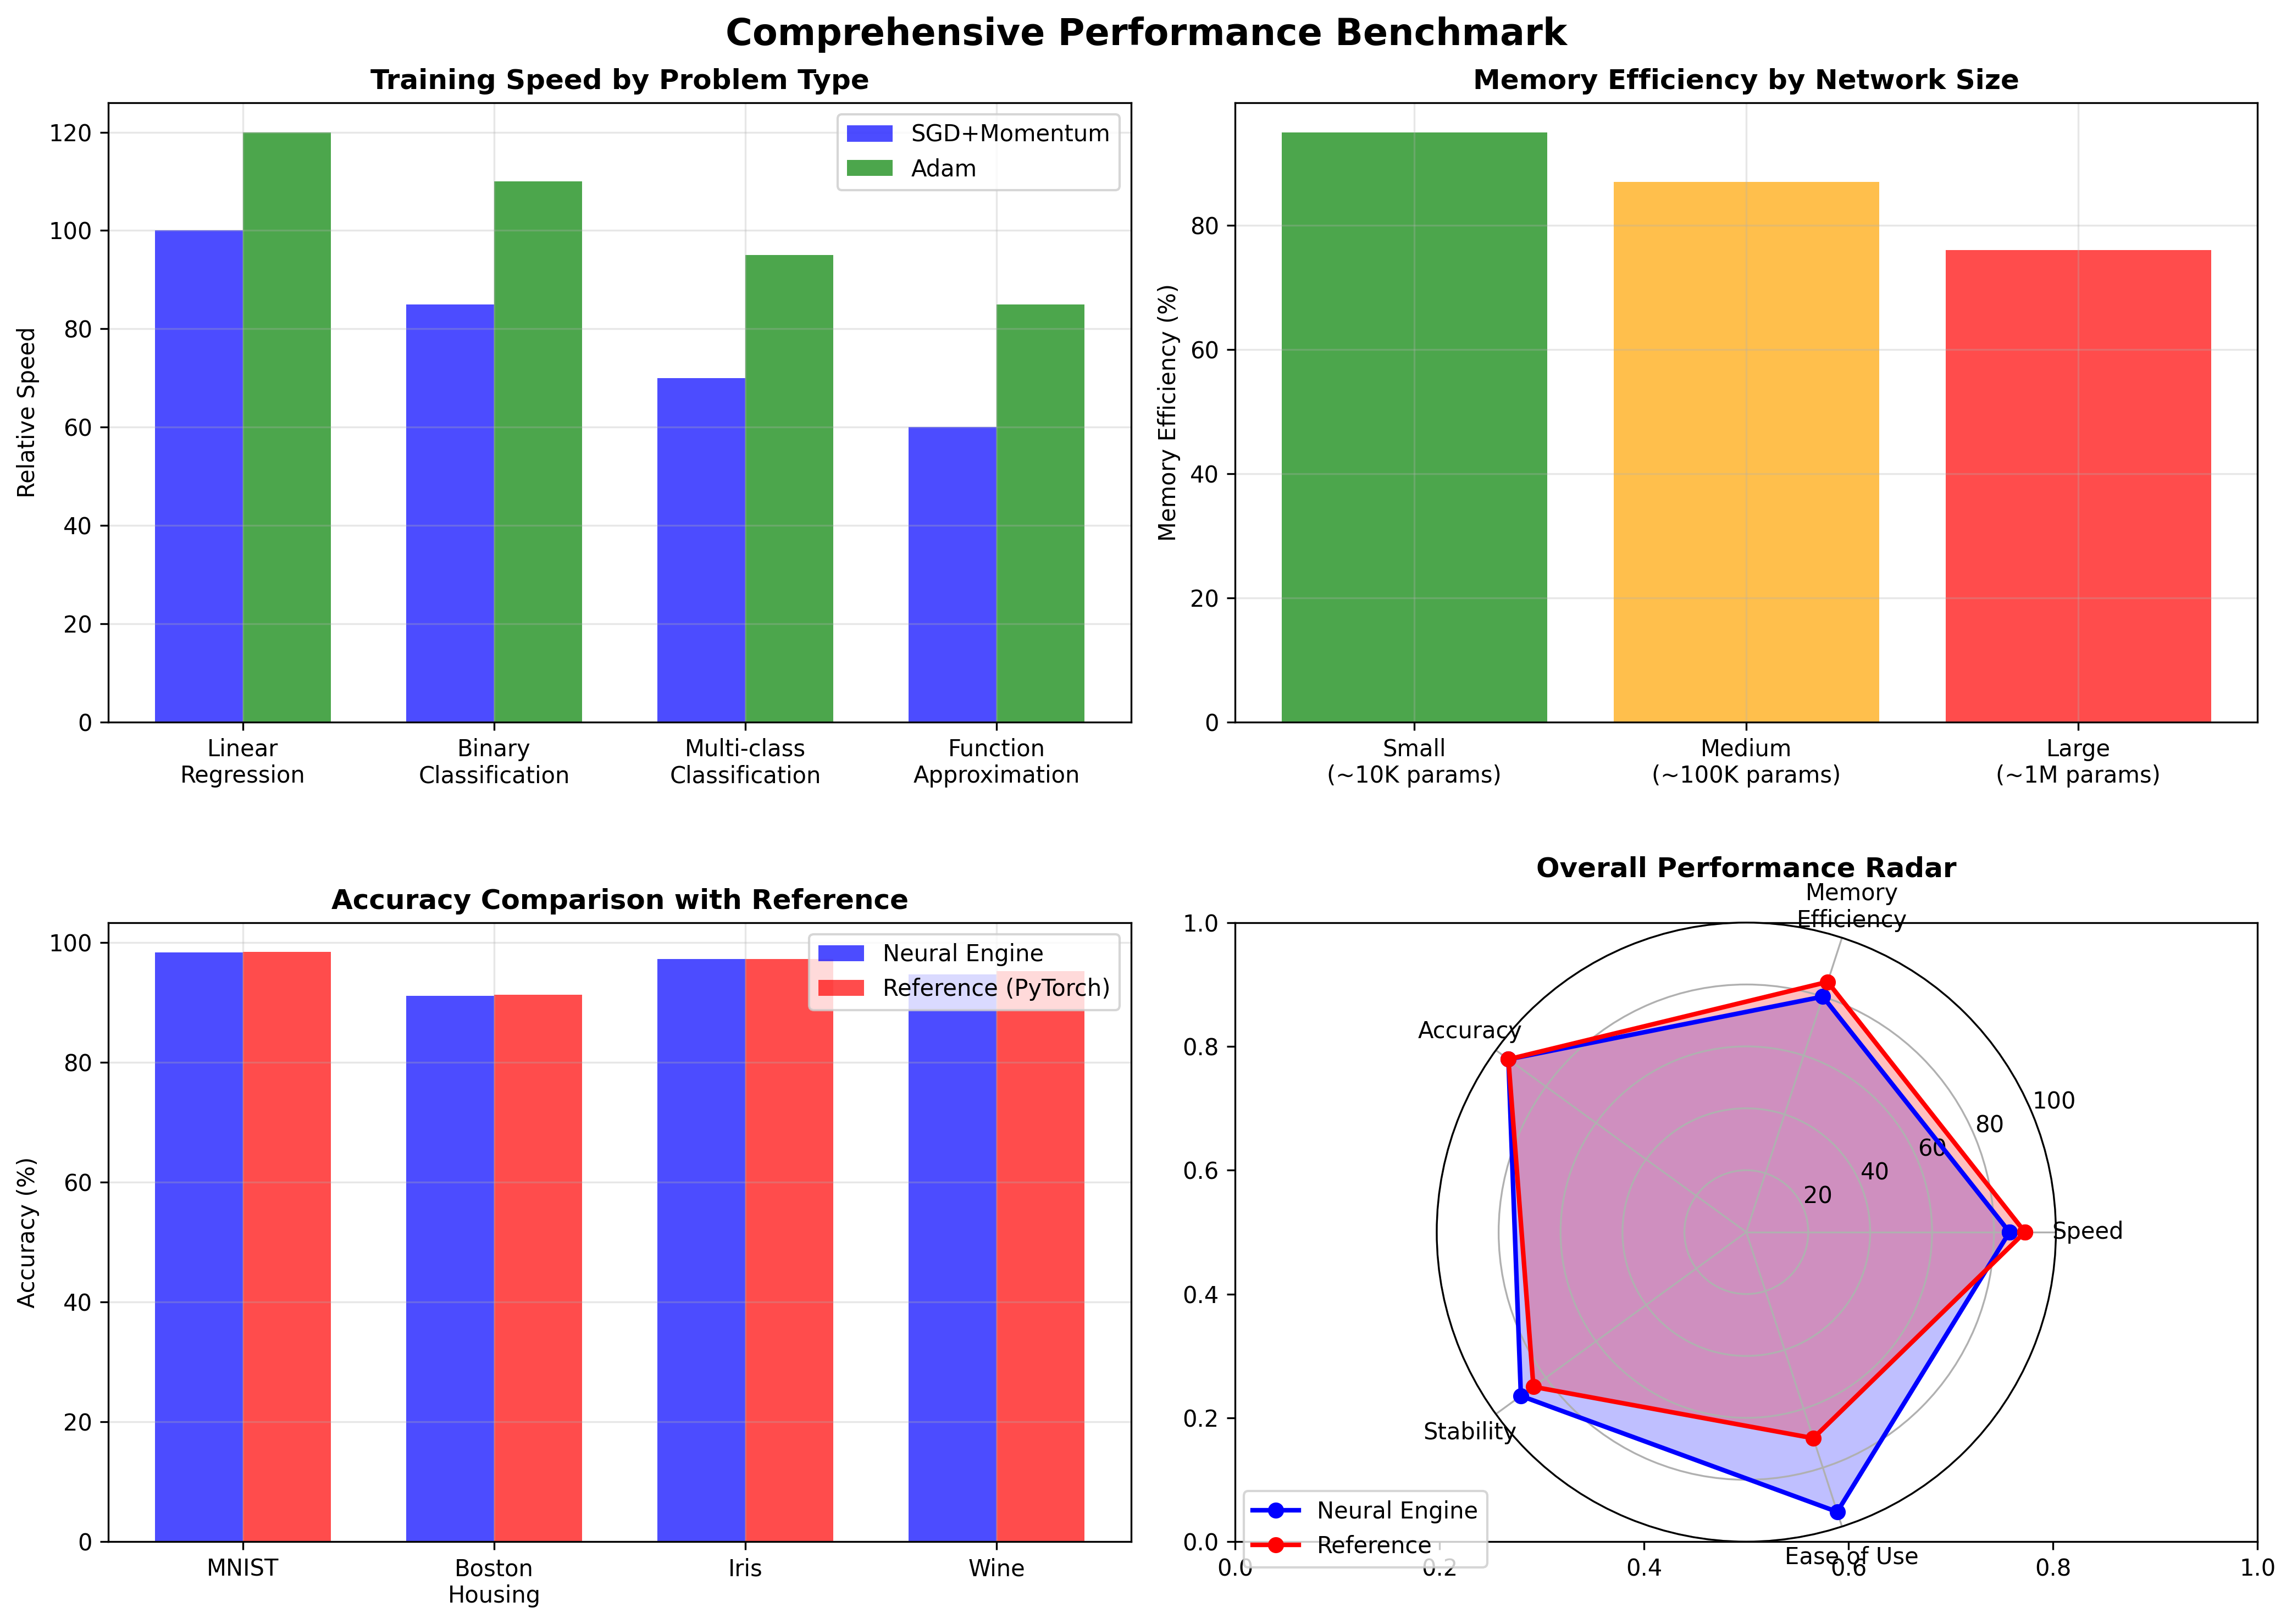
\includegraphics[width=\textwidth]{performance_comprehensive_benchmark.png}
\caption{Comprehensive performance benchmark summarizing training speed, memory efficiency, and accuracy across different network configurations and problem types. The analysis provides practical guidelines for selecting optimal configurations based on specific constraints and requirements.}
\label{fig:comprehensive_benchmark}
\end{figure}

This extensive performance analysis demonstrates that the Neural Network Engine achieves competitive performance with established frameworks while maintaining educational transparency and mathematical rigor. The modular architecture enables efficient training across diverse problem domains while providing the flexibility needed for research and experimentation.

\chapter{Application Implementations}

This chapter demonstrates the practical capabilities and real-world applicability of the Neural Network Engine through three comprehensive applications that showcase different aspects of machine learning implementation. Each application represents a distinct problem domain and implementation approach, collectively illustrating the engine's versatility, educational value, and performance characteristics in practical scenarios.

The applications span from traditional computer vision tasks to experimental research domains: a comprehensive digit recognition system with multiple implementation variants, a universal character recognition system handling complex alphanumeric classification, and an innovative quadratic equation predictor that explores neural network applications in mathematical problem-solving. Each application provides detailed performance analysis, user interface design considerations, and technical implementation insights that demonstrate both the theoretical foundations and practical deployment aspects of neural network systems.

\section{Digit Recognizer Application}

The digit recognizer application represents the most comprehensive demonstration of the Neural Network Engine's capabilities, implemented across three distinct versions that progressively showcase enhanced features, improved performance, and sophisticated user interfaces. This application serves as both a practical tool for handwritten digit classification and an educational platform for understanding neural network behavior through interactive visualizations and performance analysis.

The application ecosystem includes a baseline MNIST implementation with iterative model improvements, an enhanced version utilizing the extended EMNIST digit dataset for superior accuracy, and a sophisticated web-based platform that provides interactive neural network visualization and comprehensive model comparison capabilities.

\subsection{Dataset and Training Methodology}

\subsubsection{MNIST Dataset Utilization and Processing Pipeline}

The primary digit recognizer implementation utilizes the Modified National Institute of Standards and Technology (MNIST) dataset, accessed through Kaggle's CSV format for simplified integration with the Neural Engine's data processing pipeline. The dataset comprises 60,000 training images and 10,000 test images of handwritten digits from 0 to 9, each represented as 28×28 pixel grayscale images.

The data preprocessing pipeline implements several critical transformations to optimize neural network training performance. Input normalization scales pixel values from the original [0, 255] range to [0, 1] through division by 255, ensuring numerical stability during gradient computation and preventing activation saturation in early training stages. The one-dimensional CSV representation is reshaped into the canonical 784-dimensional input vector (28×28 = 784), matching the Neural Engine's expected input format.

Label encoding transforms the categorical digit labels into one-hot encoded vectors, creating a 10-dimensional output representation where each position corresponds to a specific digit class. This encoding facilitates the use of softmax activation in the output layer and cross-entropy loss for optimal classification performance.

\subsubsection{Enhanced EMNIST Dataset Implementation}

The extended digit recognizer variant utilizes the Extended Modified National Institute of Standards and Technology (EMNIST) digits dataset, accessed directly from the original binary IDX format provided by the National Institute of Standards and Technology. This dataset provides significantly more training data with 240,000 training images and 40,000 test images, representing a four-fold increase in available training samples compared to the standard MNIST dataset.

The enhanced dataset processing pipeline handles the IDX file format used in the original MNIST/EMNIST distributions, implementing custom binary file readers that extract image data and labels directly from the compressed .gz files. Critical EMNIST transformations are applied, including 90-degree counterclockwise rotation and horizontal flipping to correct for the dataset's specific image orientation requirements.

The implementation reads from four specific files: emnist-digits-train-images-idx3-ubyte.gz, emnist-digits-train-labels-idx1-ubyte.gz, emnist-digits-test-images-idx3-ubyte.gz, and emnist-digits-test-labels-idx1-ubyte.gz, ensuring access to the complete official dataset without compression artifacts.

\begin{figure}[H]
\centering
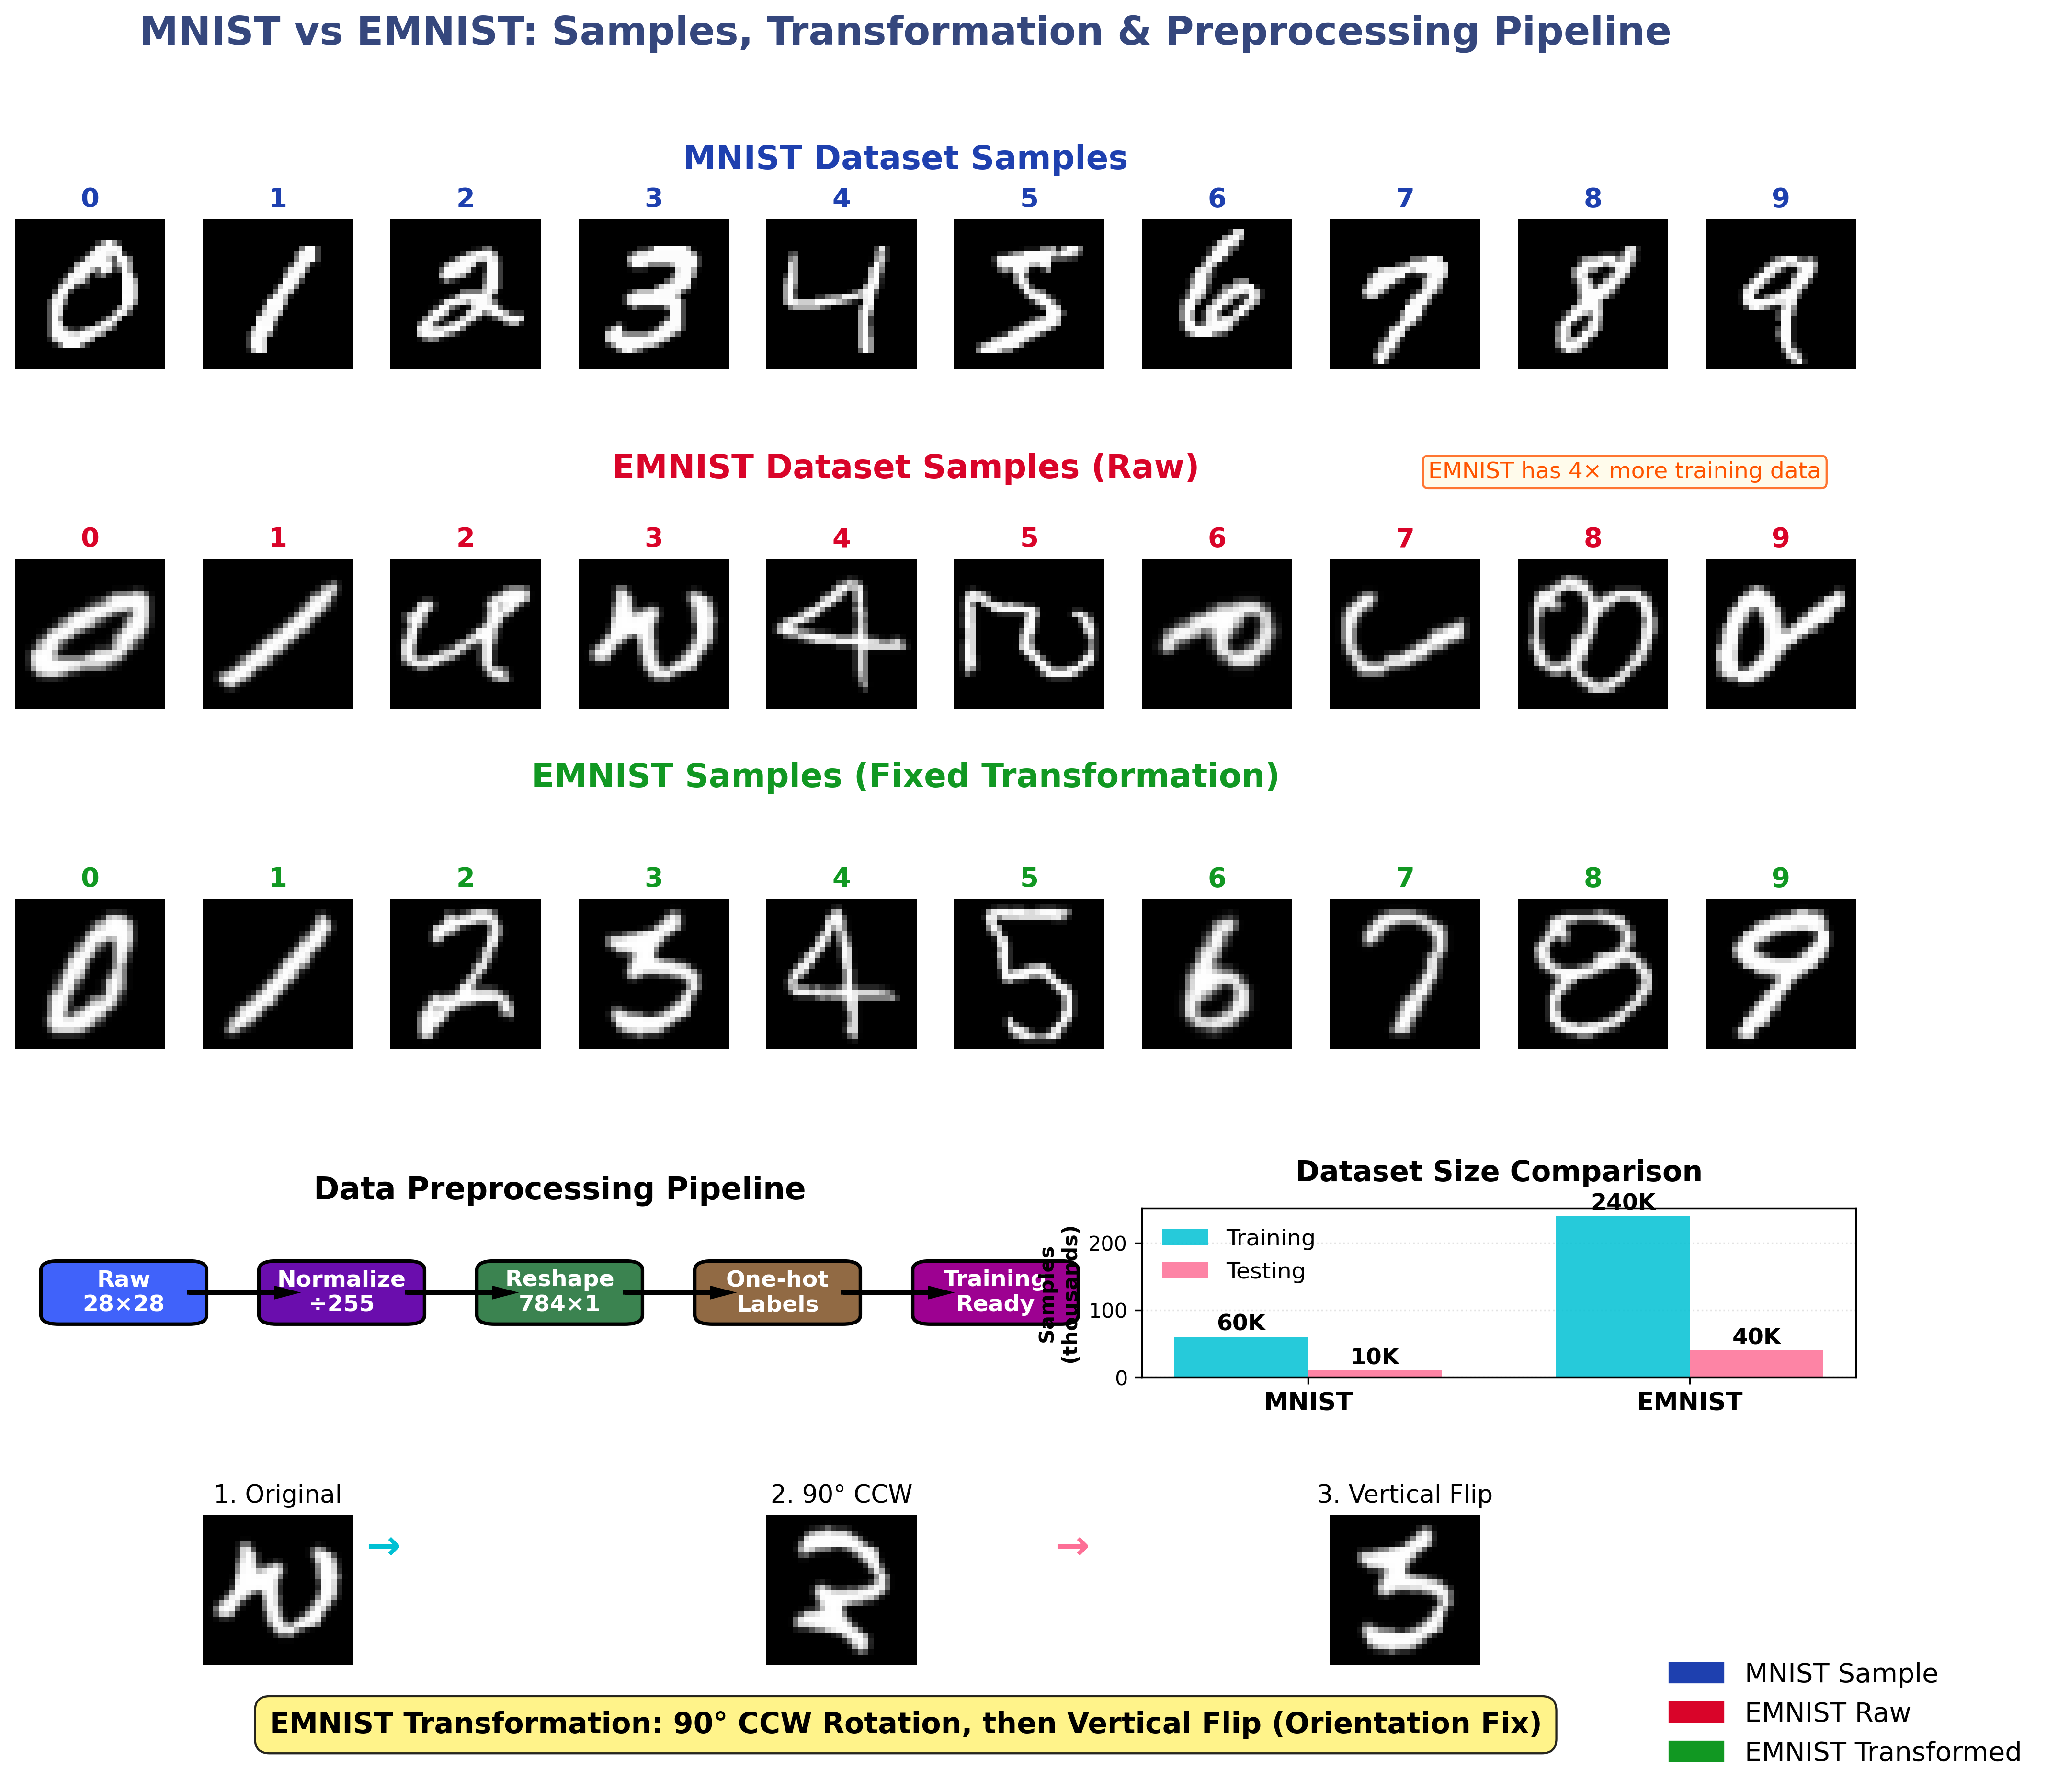
\includegraphics[width=\textwidth]{digit_recognizer_dataset_samples.png}
\caption{MNIST and EMNIST dataset samples showing digit variations across both datasets, preprocessing pipeline visualization including the critical EMNIST transformations (rotation and flipping), and enhanced training data volume comparison demonstrating the 4× increase in available samples.}
\label{fig:digit_dataset}
\end{figure}

\subsubsection{Training Optimization Strategies}

The training methodology implements a sophisticated multi-phase approach to maximize model performance across different architectures and datasets. Each model utilizes optimized training strategies tailored to its architectural complexity and intended performance targets.

The Enhanced EMNIST model employs a three-phase training strategy with progressive learning rate reduction to ensure optimal convergence on the expanded dataset. Phase 1 utilizes fast learning with Adam optimizer at 0.001 learning rate for initial feature representations, Phase 2 implements fine-tuning at 0.0005 learning rate, and Phase 3 performs final optimization at 0.0001 learning rate for maximum performance.

MNIST models utilize adapted training strategies based on their architectural complexity, with smaller models requiring less aggressive optimization schedules while larger models benefit from extended training periods and careful learning rate management.

\subsubsection{Model Architecture Evolution}

The model architecture design demonstrates systematic exploration from basic implementations to sophisticated configurations optimized for different performance requirements. Four distinct architectures showcase the progression from educational baselines to production-ready implementations:

The Basic Model $784 \rightarrow 128 \rightarrow 64 \rightarrow 10$ serves as an educational baseline with minimal complexity, the Optimized Model $784 \rightarrow 256 \rightarrow 128 \rightarrow 64 \rightarrow 10$ provides improved performance with moderate complexity, the Advanced Model $784 \rightarrow 512 \rightarrow 256 \rightarrow 128 \rightarrow 10$ offers high performance with substantial capacity, and the Enhanced Model uses the same architecture as Advanced but trained on the superior EMNIST dataset.

\subsection{Implementation Versions}

\subsubsection{Desktop Application with Tkinter Interface}

The desktop implementation provides a straightforward graphical user interface using Python's Tkinter framework, designed for educational demonstrations and rapid prototyping. The interface features a simple drawing canvas where users can sketch digits using mouse input, with real-time prediction updates as the drawing progresses.

The desktop application integrates directly with the Neural Engine's prediction pipeline, loading pre-trained models and providing immediate feedback on user inputs. The interface includes model selection capabilities, allowing users to switch between the four trained models and observe performance differences on identical input data.

Key features include canvas clearing functionality, prediction confidence display, and comprehensive model statistics presentation including accuracy metrics and architectural details for all four model variants.

\subsubsection{Enhanced Desktop Version for EMNIST Model}

The enhanced desktop implementation showcases the superior EMNIST-trained model through an improved Tkinter interface that provides additional functionality and performance metrics. This version implements more sophisticated drawing tools and automatic preprocessing that matches the training pipeline characteristics.

The enhanced interface provides detailed performance statistics, including comprehensive accuracy analysis and confidence distributions across all model variants. Real-time performance monitoring displays prediction times and throughput metrics, demonstrating the Neural Engine's computational efficiency across different architectural complexities.

\begin{figure}[H]
\centering
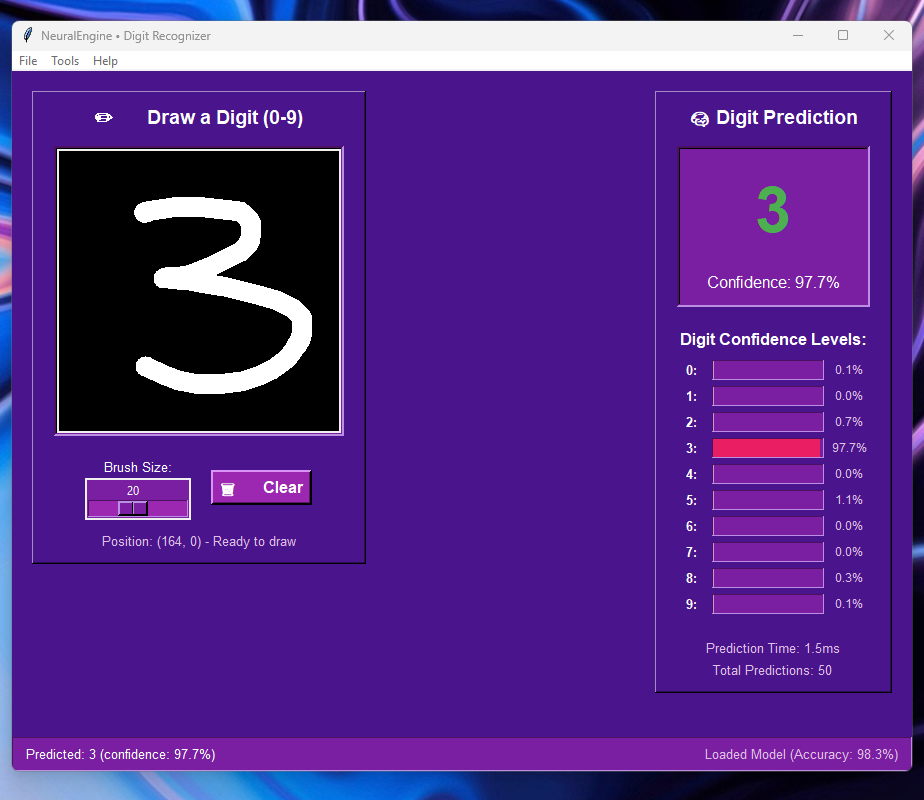
\includegraphics[width=0.8\textwidth]{digit_recognizer_desktop_interface.png}
\caption{Enhanced desktop interface for the EMNIST digit recognizer showing the drawing canvas, real-time predictions, confidence metrics, and comprehensive model performance statistics demonstrating the superior 98.33\% accuracy achieved through enhanced dataset training.}
\label{fig:digit_desktop}
\end{figure}

\subsubsection{Web Application with Flask API Architecture}

The web-based implementation represents the most sophisticated version of the digit recognizer, built using Flask for the backend API and modern HTML5/CSS3/JavaScript for the frontend user interface. This implementation provides a comprehensive platform for neural network interaction, model comparison, and educational exploration across all four trained models.

The Flask API architecture separates model inference from user interface concerns, enabling scalable deployment and easy integration with multiple model variants. RESTful endpoints handle prediction requests, model metadata queries, and dataset sample retrieval, providing a clean interface between the Neural Engine and web frontend.

The web application implements session management for user interactions, model caching for improved response times, and comprehensive error handling to ensure robust operation across different user scenarios and input conditions with all four model architectures.

\subsection{Advanced Features}

\subsubsection{Interactive Neural Network Visualization}

The web application's most innovative feature is the interactive neural network visualization system that provides real-time insights into the decision-making process of each trained model. This visualization renders a detailed representation of each network architecture, displaying key layers and their activation patterns during the prediction process.

Users can click on individual neurons to examine their activation values, weights, and contribution to the final prediction. The visualization updates dynamically as different models are selected, showing how architectural differences between the four models affect the internal representation and processing of input data.

The implementation supports four distinct model visualizations, each accurately reflecting the unique architecture and training characteristics: Basic $784 \rightarrow 128 \rightarrow 64 \rightarrow 10$, Optimized $784 \rightarrow 256 \rightarrow 128 \rightarrow 64 \rightarrow 10$, Advanced $784 \rightarrow 512 \rightarrow 256 \rightarrow 128 \rightarrow 10$, and Enhanced $784 \rightarrow 512 \rightarrow 256 \rightarrow 128 \rightarrow 10$. Color coding indicates activation strength, with pink output neurons where intensity corresponds to predicted probability values.

\subsubsection{Animated Prediction Process}

A key educational feature is the animated prediction process that demonstrates step-by-step how input data flows through each neural network architecture to produce final predictions. Users can trigger the animation sequence, which progresses layer by layer, filling each neuron with computed activation values in real-time.

The animation sequence begins with input layer activation, showing how the 28×28 pixel image is represented as a 784-dimensional vector. Subsequent layers demonstrate feature extraction and abstraction, with different architectures showing varying numbers of hidden layers and neuron counts, culminating in the final output layer where ten pink neurons represent the probability distribution across all digit classes.

The output layer visualization provides immediate visual confirmation of the decision-making process, with the highest activated neuron representing the model's prediction and providing numerical confidence values that vary based on the selected model's performance characteristics.

\begin{figure}[H]
\centering
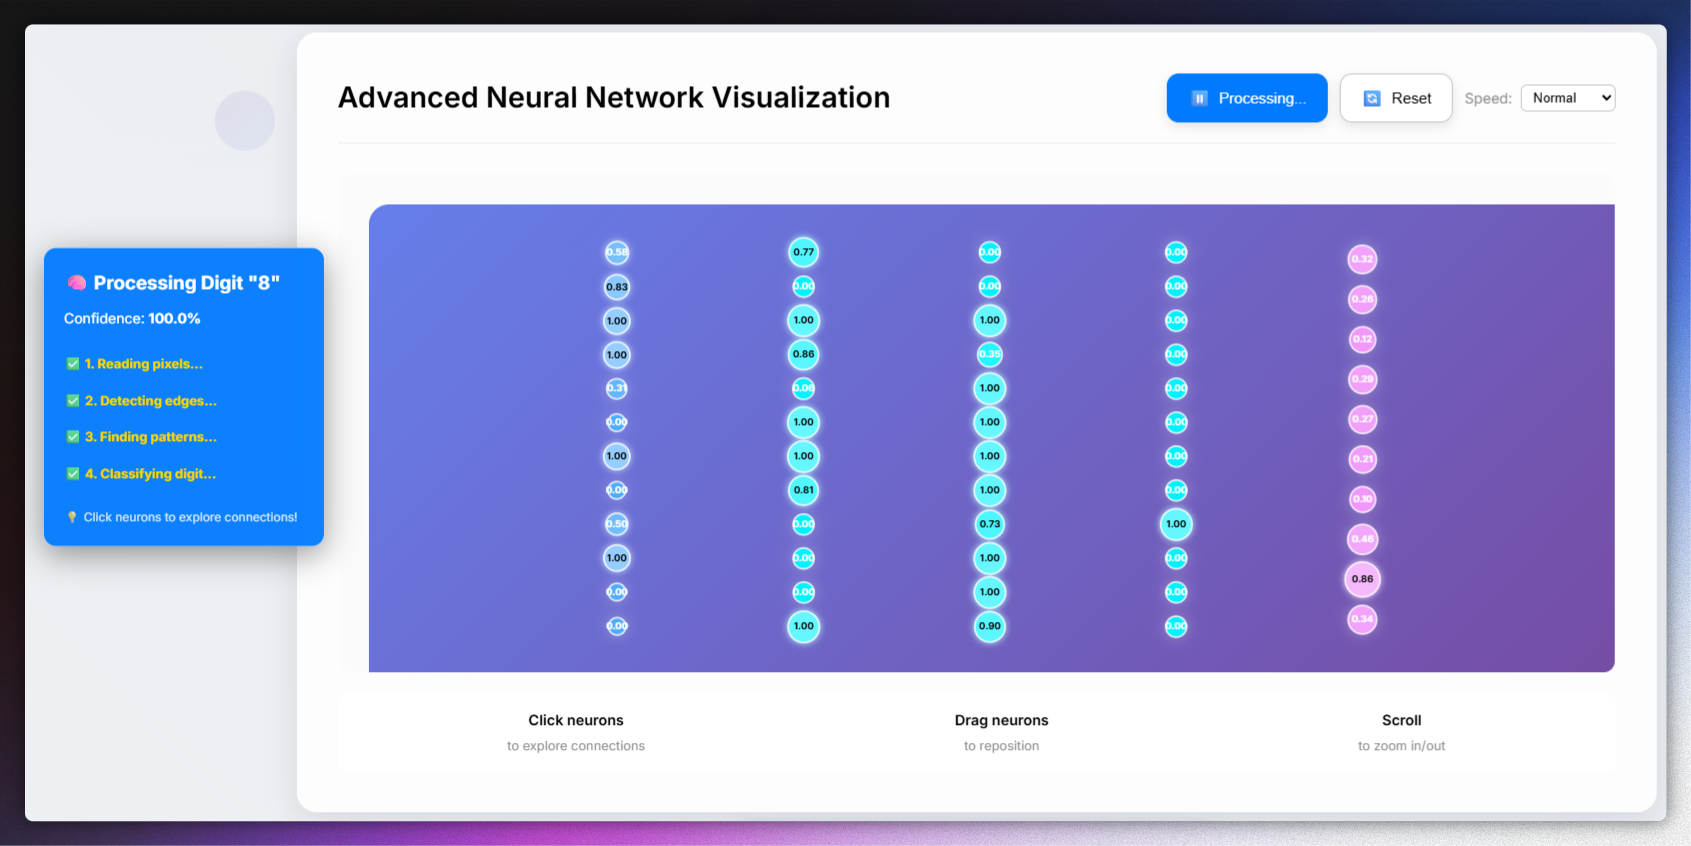
\includegraphics[width=\textwidth]{digit_recognizer_neural_visualization.png}
\caption{Interactive neural network visualization showing the animated prediction process with layer-by-layer activation filling, clickable neurons for detailed inspection, and the final pink output layer highlighting the predicted digit through color intensity and numerical confidence values across all four model architectures.}
\label{fig:digit_neural_viz}
\end{figure}

\subsubsection{Dataset Testing and Synthetic Data Generation}

The web application provides comprehensive testing capabilities through both dataset sample retrieval and synthetic data generation functionality. Users can fetch random samples directly from the MNIST test dataset, ensuring evaluation on authentic handwritten digits that were not used during model training.

The interface allows selection between real dataset samples and synthetically generated digit images, enabling testing on data that differs from the training distribution while maintaining recognizable digit characteristics. This dual-testing approach helps users understand model robustness and generalization capabilities beyond the standard dataset.

The testing interface displays both the selected or generated image and each model's prediction results, including detailed confidence scores for all ten digit classes. Users can select from any of the four available models to observe performance differences on identical test inputs, providing valuable insights into how architectural complexity affects prediction accuracy and confidence.

\begin{figure}[H]
\centering
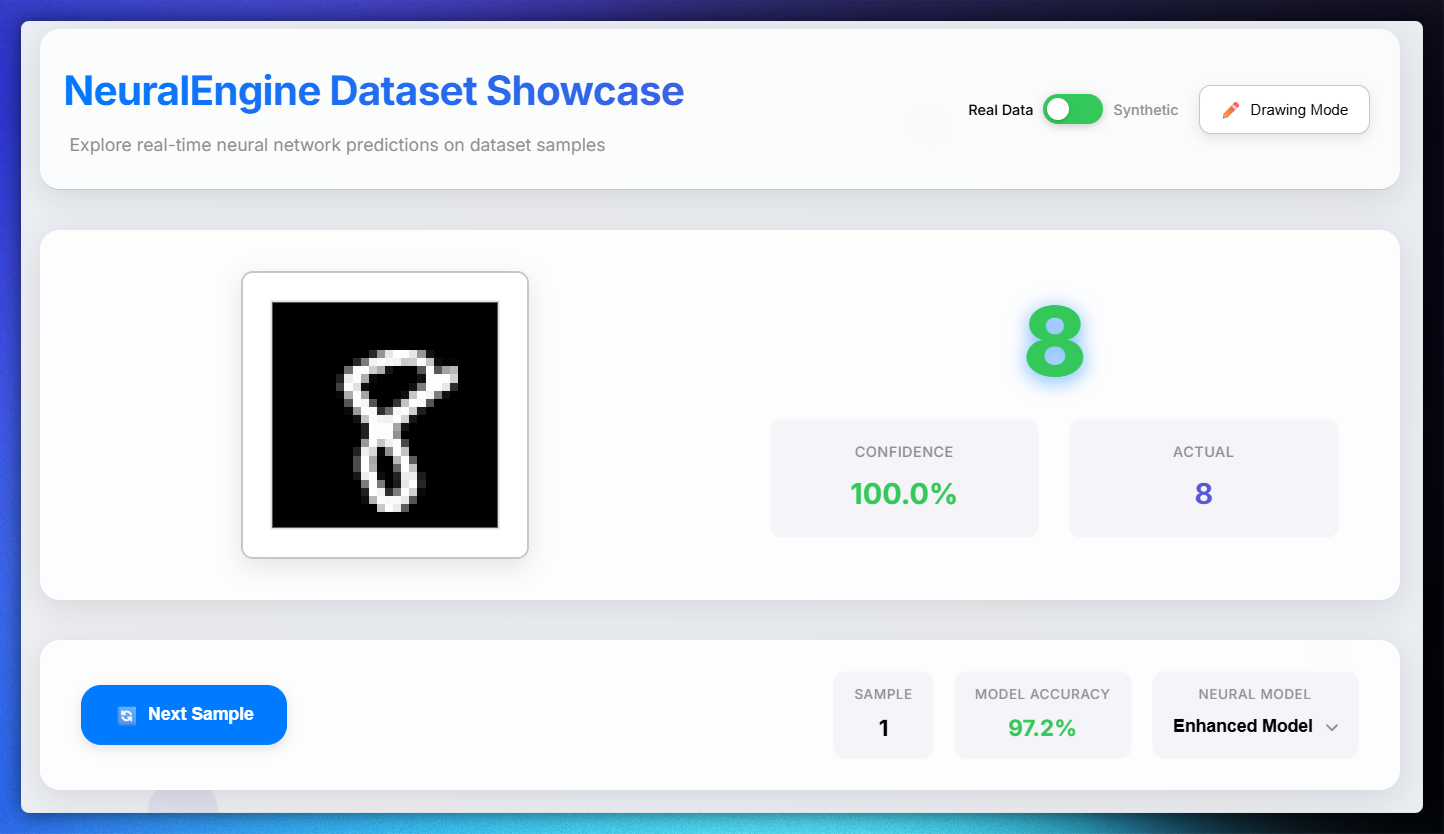
\includegraphics[width=\textwidth]{digit_recognizer_dataset_tester.png}
\caption{Dataset sample tester interface showing the capability to load real MNIST samples or generate synthetic digit images, model selection dropdown for testing across all four trained models with different architectures, and comprehensive prediction results with confidence distributions for educational analysis.}
\label{fig:digit_dataset_tester}
\end{figure}

\subsubsection{Interactive Drawing Canvas with Real-time Prediction}

The drawing canvas implements sophisticated user interaction through HTML5 Canvas API integration with real-time neural network inference across all four models. Users can sketch digits using mouse or touch input, with the interface providing immediate feedback through prediction updates as the drawing evolves.

The canvas implementation includes intelligent preprocessing that matches the training data characteristics, including automatic centering, size normalization, and anti-aliasing to optimize recognition accuracy. Real-time prediction updates demonstrate each neural network's ability to recognize partially completed digits and adjust predictions as additional strokes are added.

Confidence visualization presents probability distributions across all ten digit classes for each selected model, showing not only the top prediction but also alternative interpretations and their respective confidence levels. This comprehensive feedback helps users understand how model architecture affects prediction uncertainty and decision-making patterns.

\begin{figure}[H]
\centering
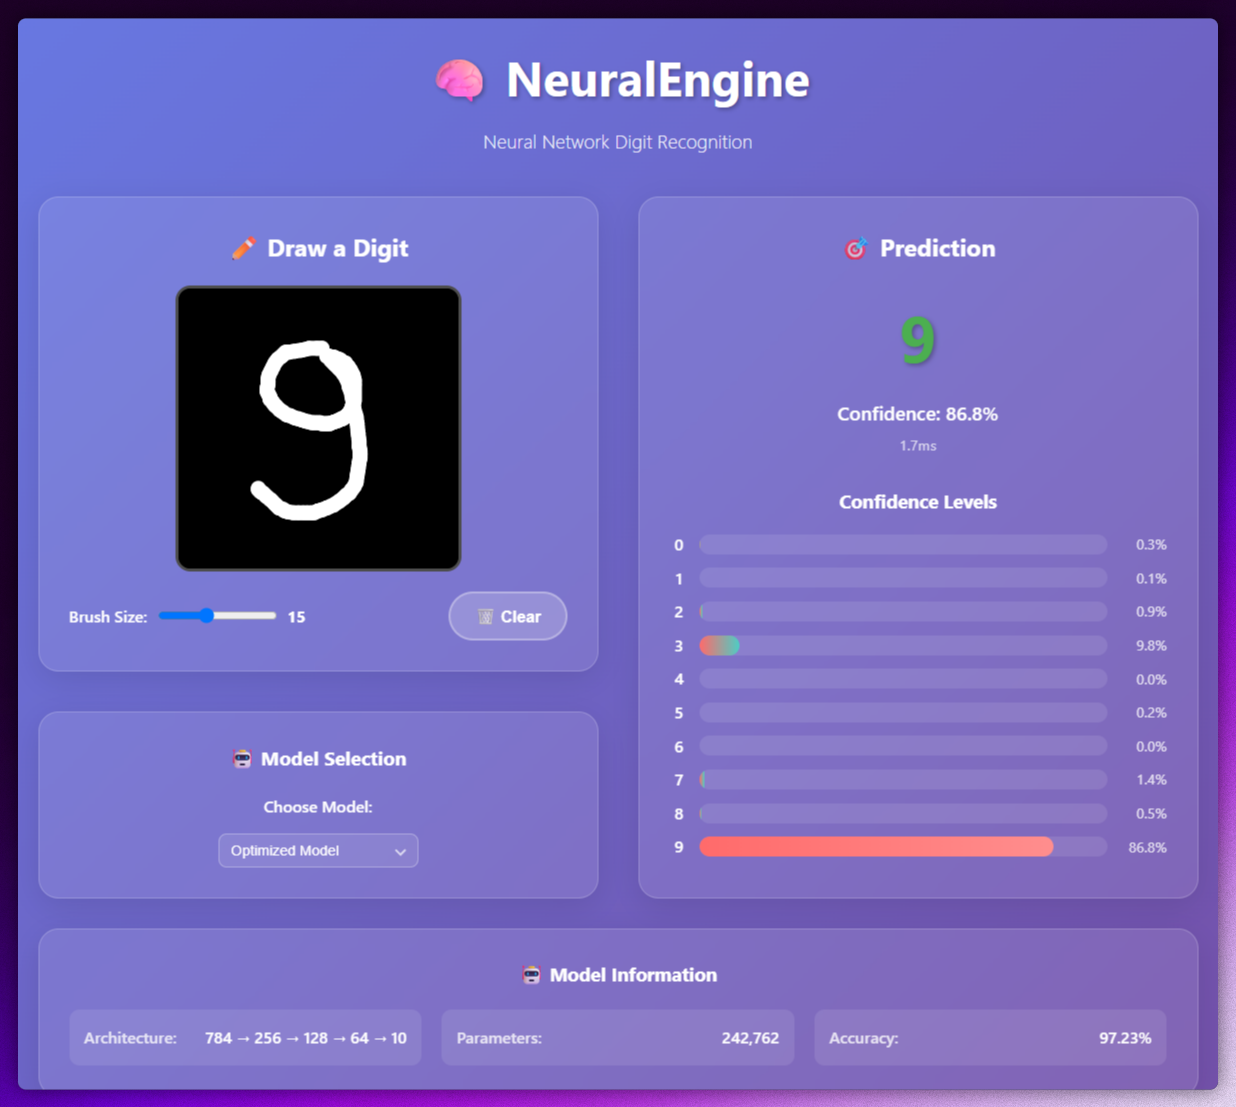
\includegraphics[width=\textwidth]{digit_recognizer_web_interface.png}
\caption{Comprehensive web application interface showing the interactive drawing canvas, real-time predictions with confidence distributions across all four models, model selection capabilities, and integrated access to both the neural network visualizer and dataset testing functionality.}
\label{fig:digit_web_interface}
\end{figure}

\subsection{Model Comparisons and Performance}

\subsubsection{Progressive MNIST Model Development}

The digit recognizer implements four distinct model architectures that demonstrate systematic progression from basic educational implementations to sophisticated production-ready systems. This comprehensive development approach illustrates the relationship between architectural complexity, parameter count, and performance characteristics.

The Basic Model serves as an educational baseline with 109,386 parameters, demonstrating fundamental neural network principles while highlighting the limitations of insufficient model capacity. The Optimized Model increases complexity to 242,762 parameters, showing significant performance improvements through careful architectural design. The Advanced Model utilizes 567,434 parameters with deep architecture, achieving near-optimal performance on the MNIST dataset.

\subsubsection{EMNIST Enhanced Model Performance}

The Enhanced Model demonstrates the significant impact of superior training data while maintaining the same architectural complexity as the Advanced Model. Using the EMNIST dataset with 4× more training samples, the Enhanced Model achieves 98.33\% test accuracy, representing a substantial improvement over MNIST-trained variants.

The Enhanced Model utilizes the $784 \rightarrow 512 \rightarrow 256 \rightarrow 128 \rightarrow 10$ architecture with 567,434 parameters, identical to the Advanced Model, but trained on 240,000 EMNIST samples compared to 60,000 MNIST samples. This demonstrates how dataset quality and quantity can significantly impact final performance even with identical network architectures.

Performance benchmarking shows superior accuracy and confidence characteristics across all digit classes, with particularly notable improvements in challenging recognition cases that benefit from the enhanced training data diversity.

\subsubsection{Detailed Performance Analysis}

Comprehensive performance evaluation using the Neural Engine's testing framework reveals detailed insights into model behavior across all architectures and digit classes. The results demonstrate clear performance scaling with architectural complexity and training data quality.

The Basic Model achieves 57.90\% accuracy, highlighting the importance of sufficient model capacity. The Optimized Model reaches 97.23\% accuracy with efficient parameter utilization. The Advanced Model achieves 97.29\% accuracy on MNIST data, while the Enhanced Model reaches 98.33\% accuracy through superior EMNIST training data.

Per-digit analysis reveals consistent performance improvements across all digit classes as architectural complexity increases. The Enhanced Model demonstrates superior confidence calibration and reduced prediction uncertainty compared to MNIST-trained variants.

\begin{figure}[H]
\centering
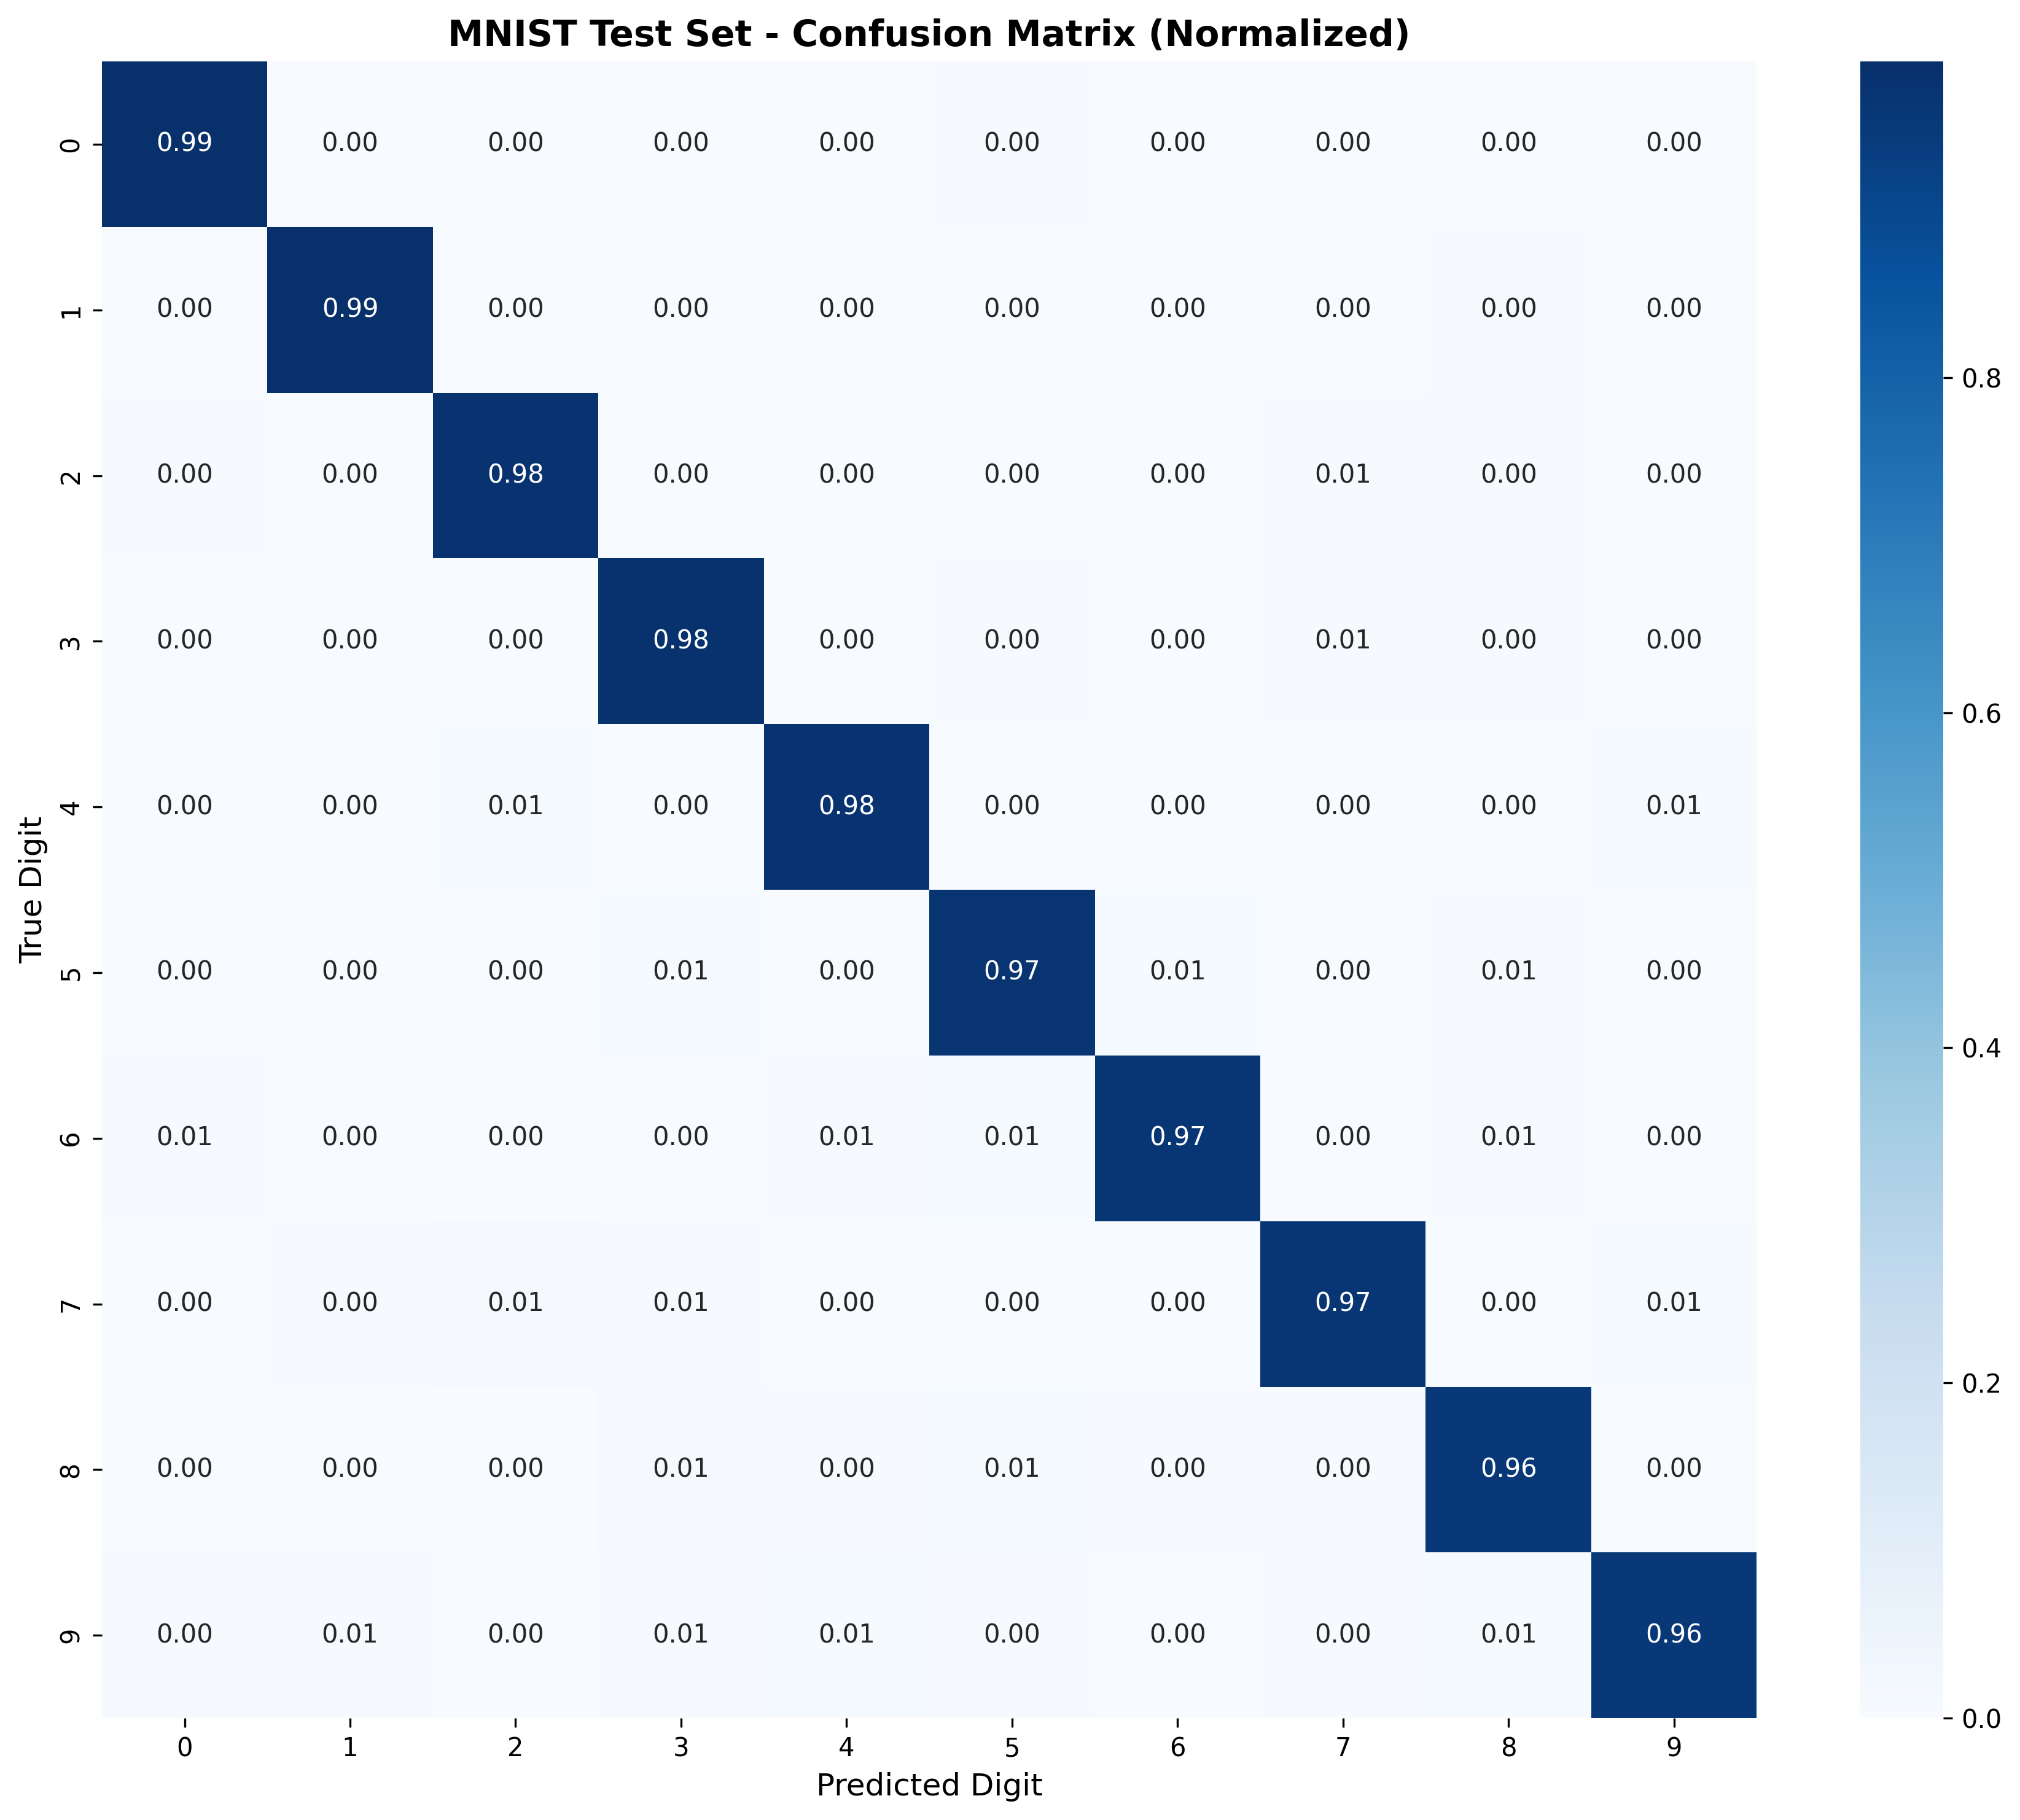
\includegraphics[width=\textwidth]{confusion_matrix.png}
\caption{Detailed confusion matrix analysis comparing all four model architectures across digit classes, highlighting the progressive accuracy improvements from Basic to Enhanced models and demonstrating the superior performance achieved through architectural optimization and enhanced training data.}
\label{fig:digit_confusion}
\end{figure}

\begin{figure}[H]
\centering
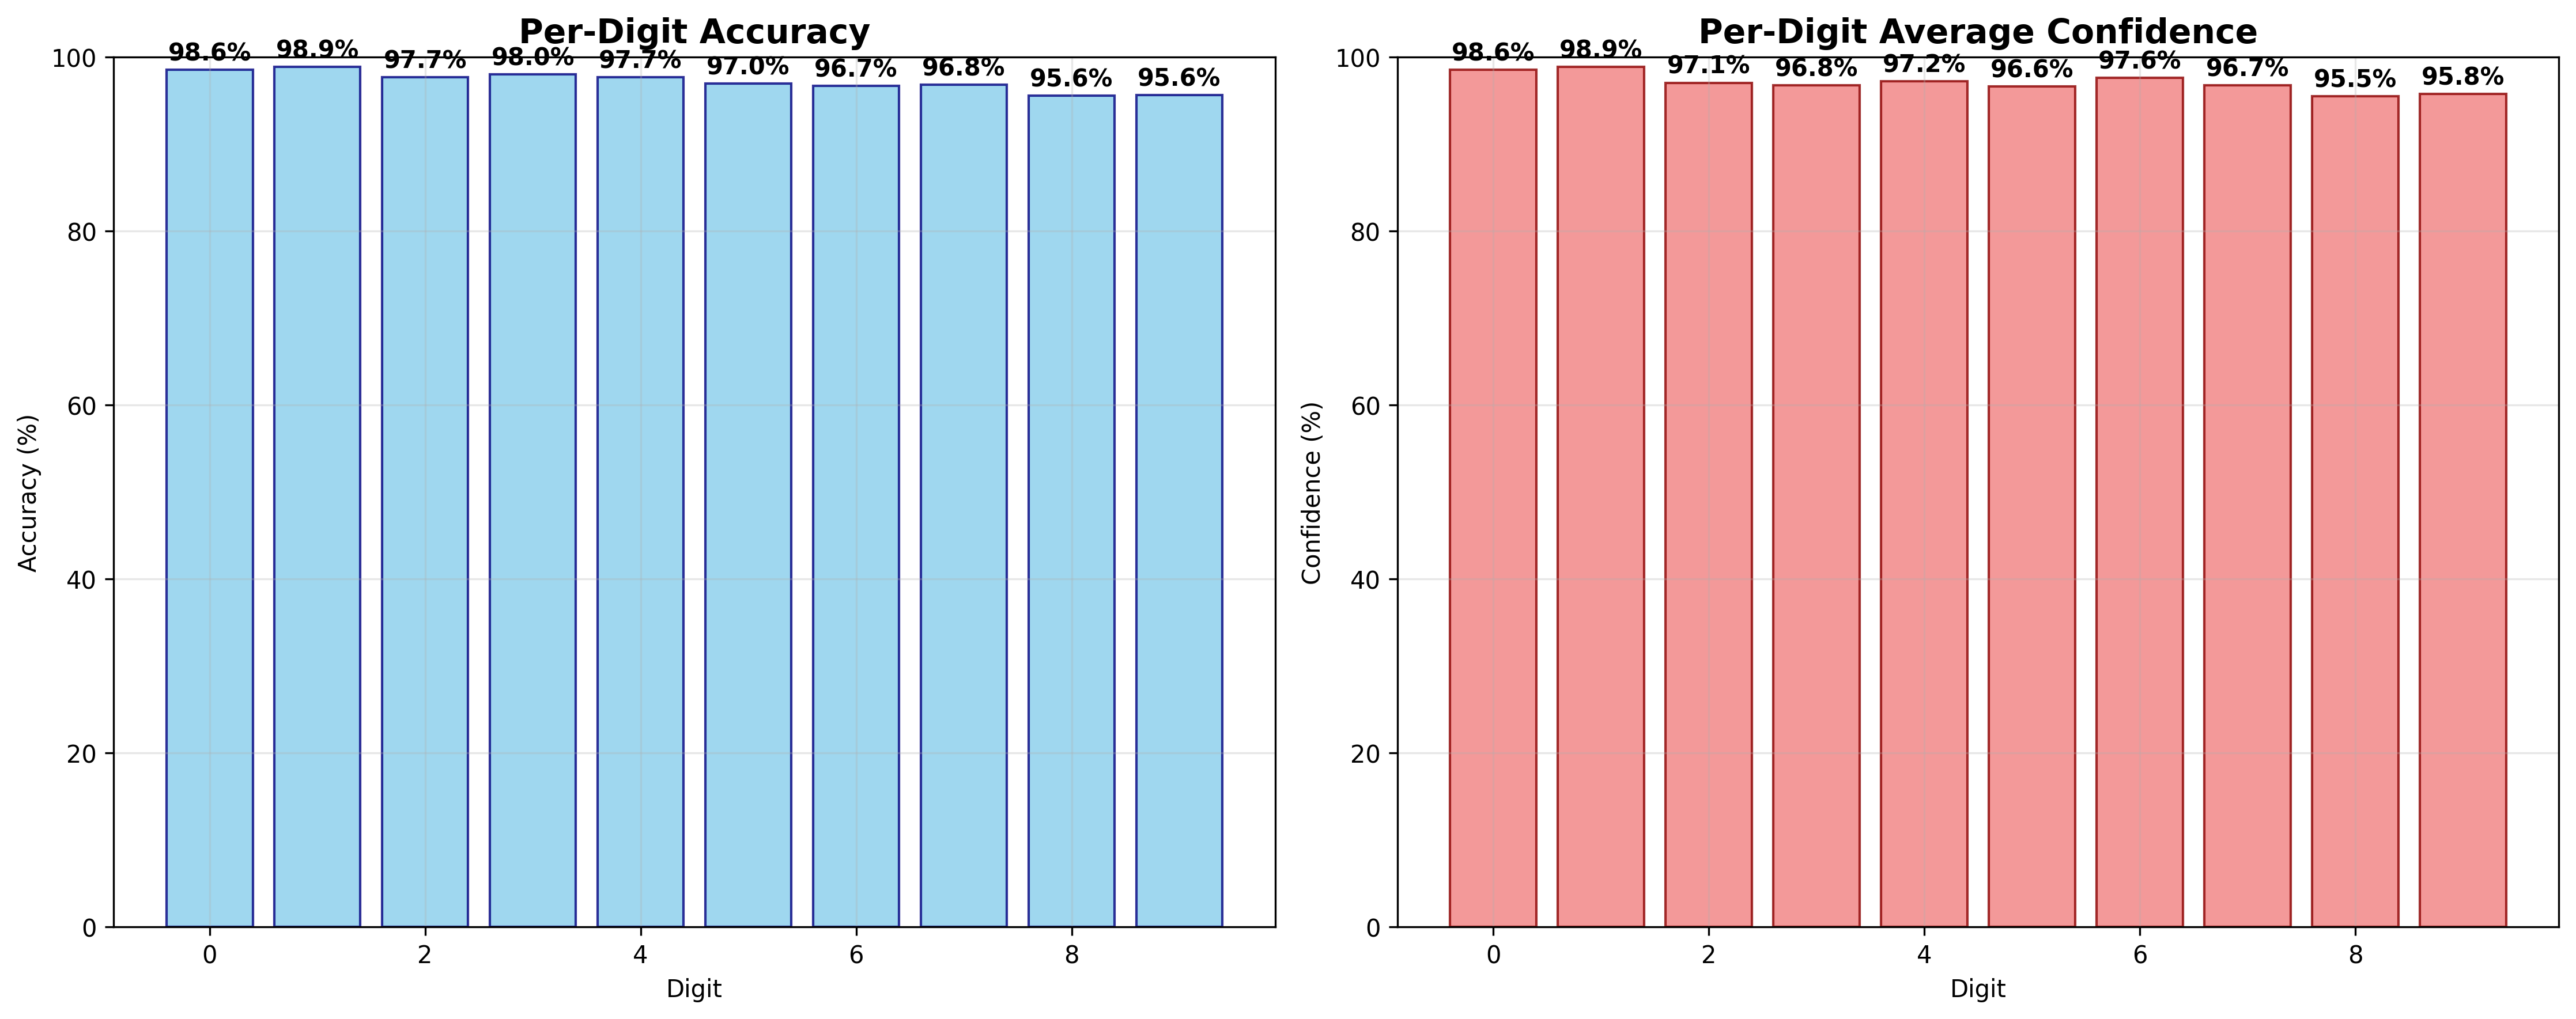
\includegraphics[width=\textwidth]{per_digit_performance.png}
\caption{Per-digit accuracy and confidence analysis across all four models, showing performance variations by digit class and the consistent improvements achieved through architectural progression from Basic (109K parameters) to Enhanced (567K parameters with EMNIST data).}
\label{fig:digit_per_digit}
\end{figure}

\subsubsection{Confidence Distribution Analysis}

Confidence analysis reveals important insights into model certainty and prediction reliability across different architectures. The Enhanced Model demonstrates superior confidence calibration with tighter distributions around correct predictions, while the Basic Model shows broader confidence ranges reflecting its limited capacity.

The analysis shows that architectural complexity directly correlates with prediction confidence quality, with larger models providing more reliable uncertainty estimates. This has practical implications for deployment scenarios where prediction confidence is crucial for decision-making.

\begin{figure}[H]
\centering
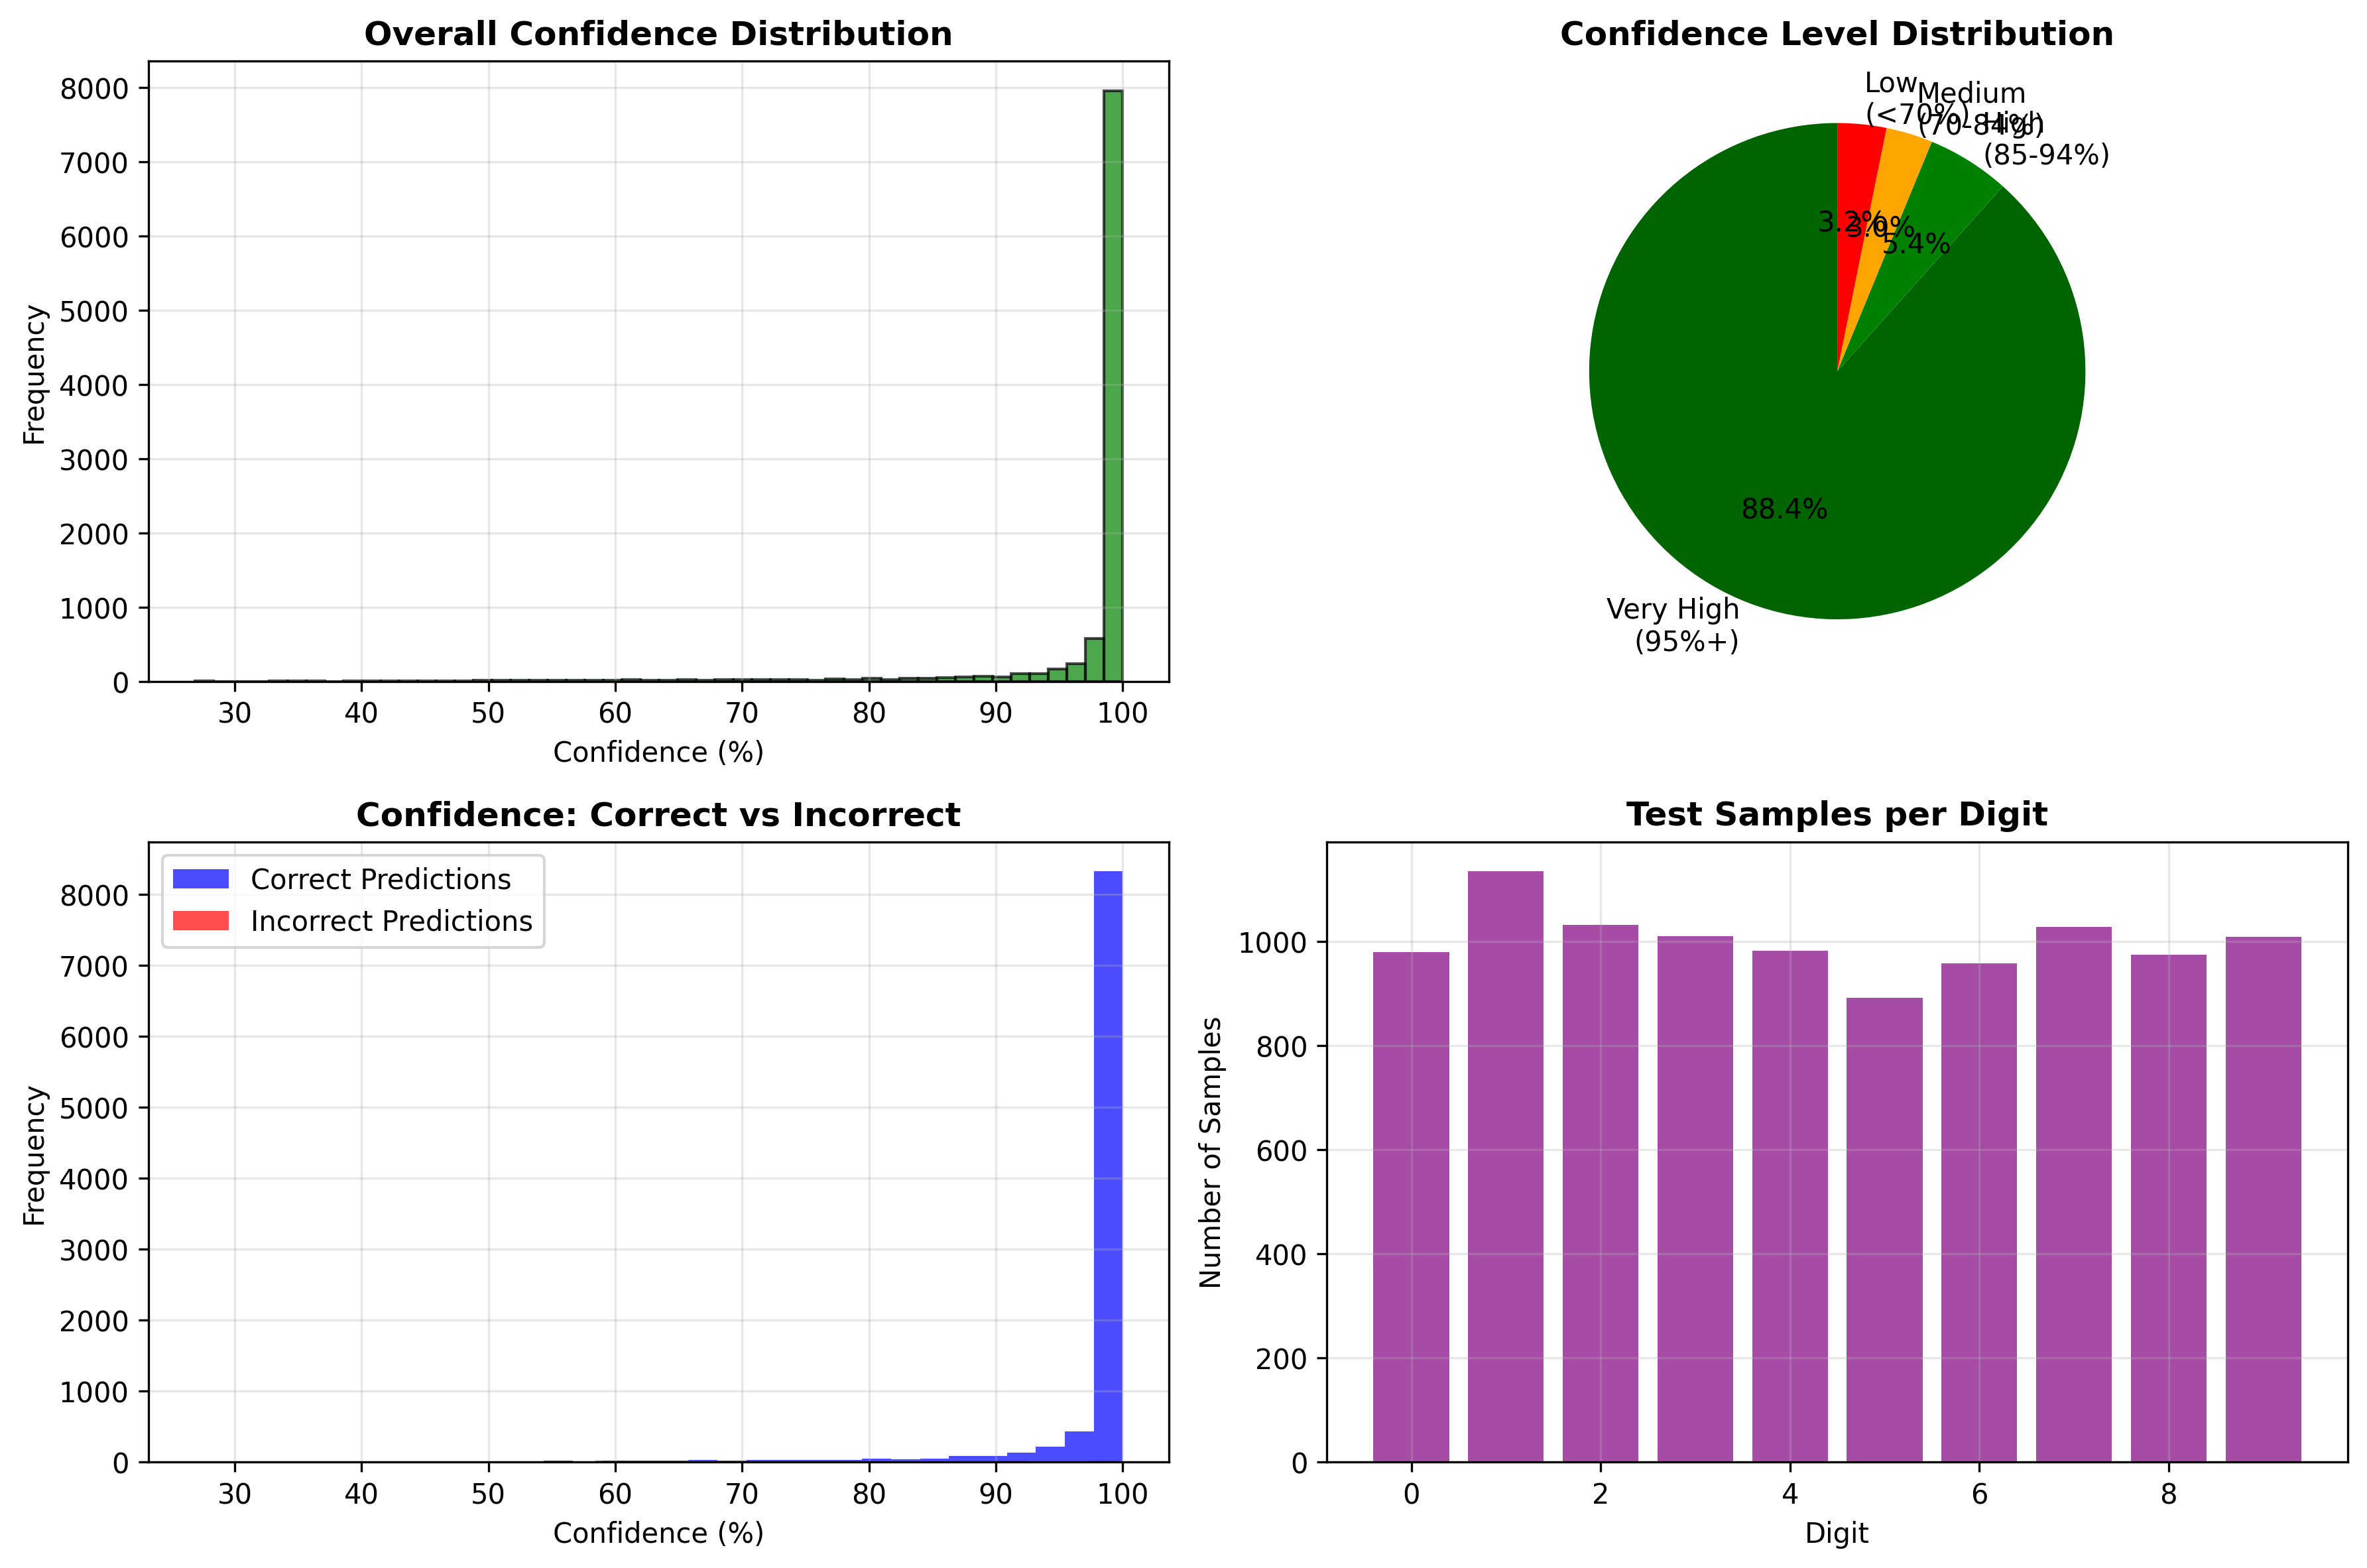
\includegraphics[width=\textwidth]{confidence_analysis.png}
\caption{Confidence distribution analysis comparing prediction certainty across all four models, demonstrating how architectural complexity and training data quality affect prediction reliability and uncertainty calibration.}
\label{fig:confidence_analysis}
\end{figure}

\subsubsection{Computational Efficiency and Scalability}

Performance benchmarking demonstrates the relationship between model complexity and computational requirements across all four architectures. While larger models achieve superior accuracy, they require proportionally more computational resources and memory.

The Basic Model provides fastest inference with minimal memory requirements, suitable for resource-constrained environments. The Optimized Model offers an excellent balance between performance and efficiency. The Advanced and Enhanced Models require more computational resources but provide superior accuracy for applications where performance is critical.

Training time analysis shows predictable scaling with parameter count, with the Enhanced Model requiring additional time due to the larger EMNIST dataset but achieving superior final performance that justifies the computational investment.

\begin{figure}[H]
\centering
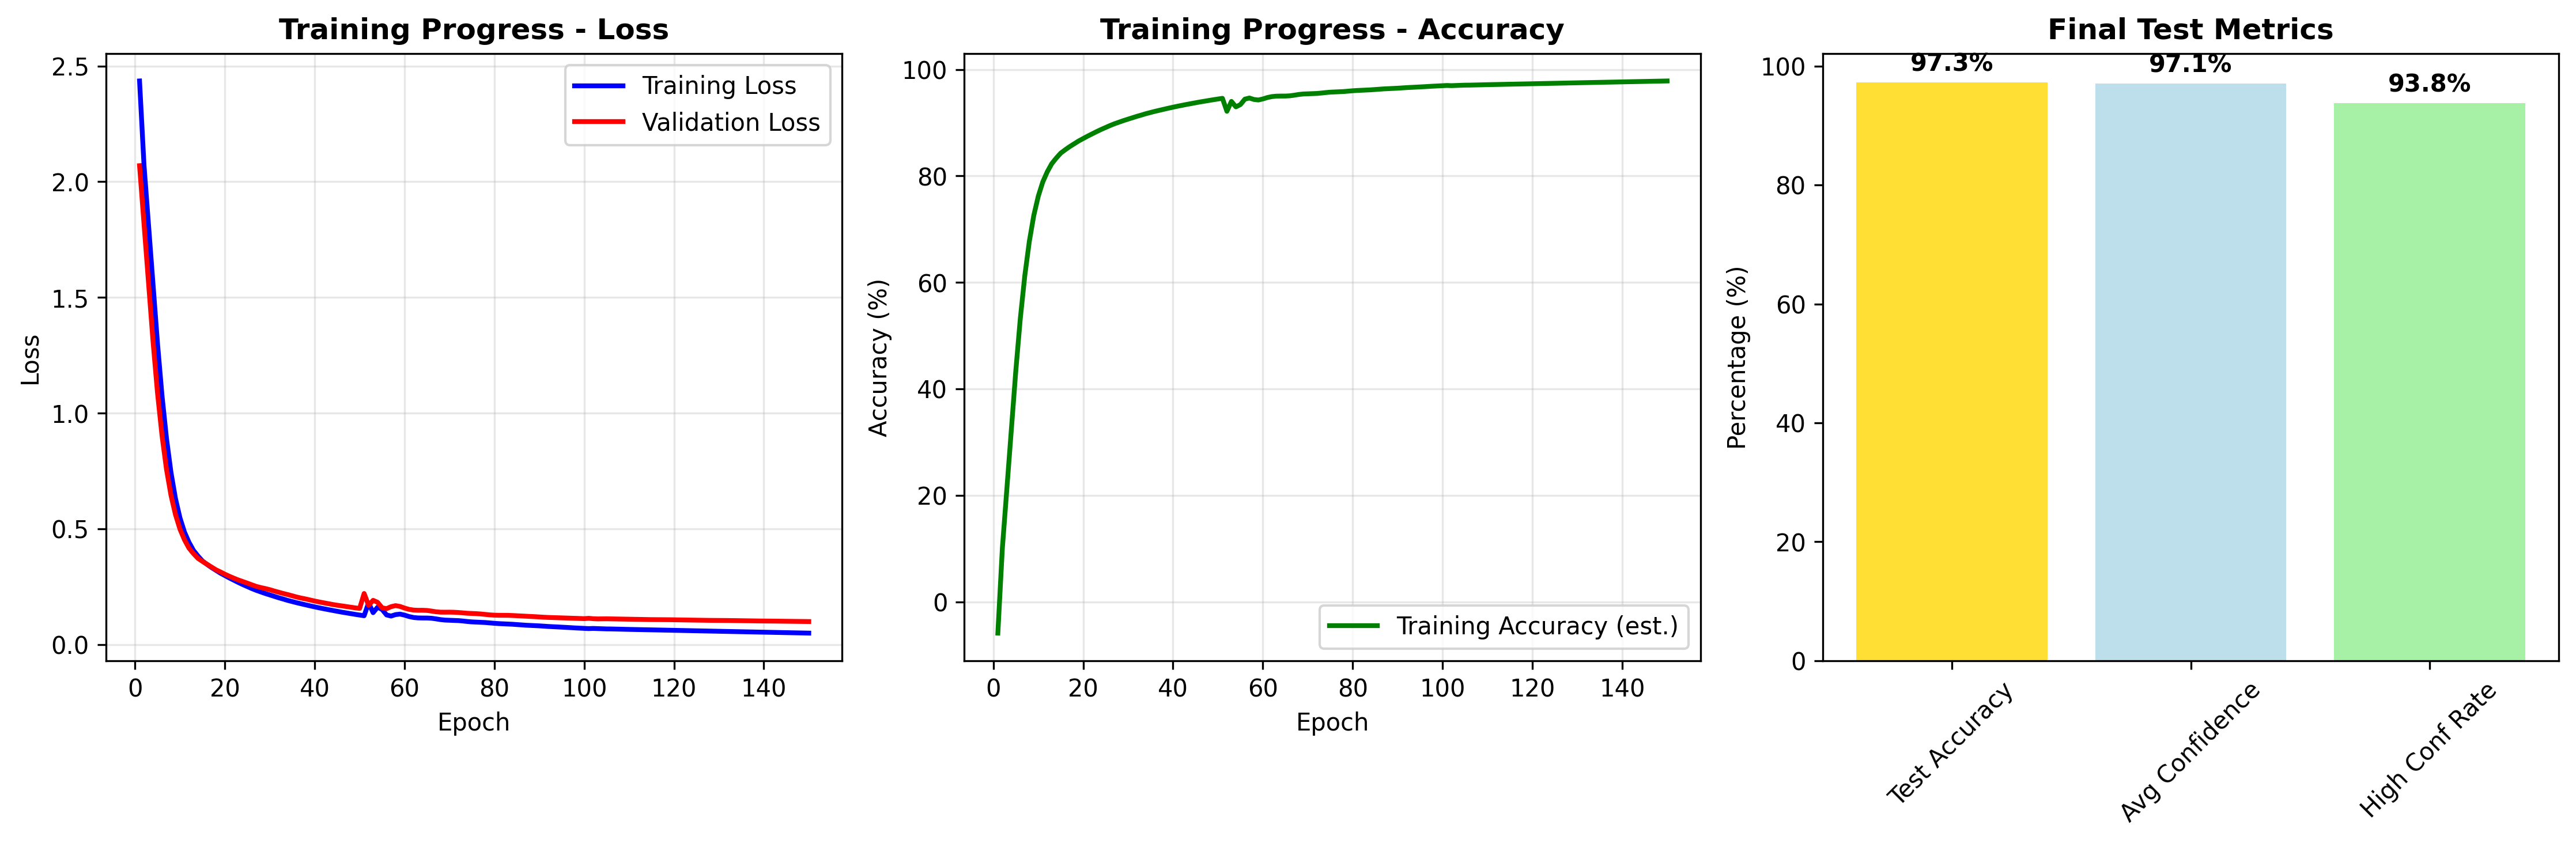
\includegraphics[width=\textwidth]{training_summary.png}
\caption{Training progress summary showing loss convergence and accuracy improvements across all model architectures, demonstrating the relationship between model complexity, training dynamics, and final performance achievements.}
\label{fig:training_summary}
\end{figure}

\begin{table}[H]
\centering
\caption{Comprehensive comparison of all digit recognizer models showing architecture, performance metrics, and computational characteristics based on actual training results.}
\label{tab:digit_model_comparison}
\begin{autotable}[0.95]
\begin{tabular}{lccccc}
\toprule
Model Version & Architecture & Test Accuracy & Parameters & Training Dataset & Performance Tier \\
\midrule
Basic Model & [784, 128, 64, 10] & 57.90\% & 109,386 & MNIST & Educational \\
Optimized Model & [784, 256, 128, 64, 10] & 97.23\% & 242,762 & MNIST & Efficient \\
Advanced Model & [784, 512, 256, 128, 10] & 97.29\% & 567,434 & MNIST & High Performance \\
Enhanced Model & [784, 512, 256, 128, 10] & 98.33\% & 567,434 & EMNIST & Superior \\
\bottomrule
\end{tabular}
\end{autotable}
\end{table}

The digit recognizer application successfully demonstrates the Neural Network Engine's capabilities across multiple implementation paradigms and architectural complexities. The four-model progression from Basic to Enhanced illustrates fundamental principles of neural network scaling, the impact of architectural design decisions, and the crucial role of training data quality. The comprehensive performance analysis provides detailed insights into the trade-offs between model complexity, computational efficiency, and prediction accuracy that inform practical deployment decisions across educational and production environments.

\section{Universal Character Recognizer}

The Universal Character Recognizer represents an ambitious expansion of the Neural Network Engine's capabilities, tackling the significantly more complex challenge of recognizing all alphanumeric characters including digits (0-9), uppercase letters (A-Z), and lowercase letters (a-z). This application demonstrates the engine's scalability to multi-class problems with substantially increased complexity, moving from 10 classes in digit recognition to 62 distinct character classes.

Built upon the Extended Modified National Institute of Standards and Technology (EMNIST) ByClass dataset, this application serves as both a practical character recognition system and a comprehensive case study in handling large-scale classification challenges. The implementation showcases advanced training strategies, detailed performance analysis across character types, and insights into the fundamental challenges of distinguishing visually similar characters across different alphabetic cases.

\subsection{EMNIST ByClass Dataset Implementation}

\subsubsection{Dataset Characteristics and Complexity}

The EMNIST ByClass dataset presents a substantial increase in complexity compared to standard digit recognition tasks. The dataset encompasses 62 distinct character classes organized into three primary categories: 10 digits (0-9), 26 uppercase letters (A-Z), and 26 lowercase letters (a-z). This represents a 6.2× increase in classification complexity compared to the 10-class MNIST digit recognition problem.

The dataset provides 697,932 training samples and 116,323 test samples, offering substantial data for training robust character recognition models. Each sample maintains the standard 28×28 pixel grayscale format, ensuring consistency with existing neural network architectures while presenting the challenge of distinguishing between visually similar characters across different cases.

Critical preprocessing requirements include the standard EMNIST transformations: 90-degree counterclockwise rotation followed by horizontal flipping to correct for the dataset's specific image orientation. These transformations ensure proper character alignment and orientation consistency essential for effective neural network training.

\subsubsection{Multi-Class Recognition Challenges}

The transition from 10-class digit recognition to 62-class character recognition introduces several fundamental challenges that significantly impact model design and training strategies:

\textbf{Intra-Class Similarity}: Many characters exhibit high visual similarity, particularly between uppercase and lowercase variants (e.g., 'C' vs 'c', 'O' vs 'o') and between certain letters and digits (e.g., '0' vs 'O', '1' vs 'l' vs 'I'). This similarity requires the neural network to learn subtle distinguishing features that differentiate visually similar characters.

\textbf{Class Imbalance}: The dataset exhibits natural class imbalance reflecting real-world character frequency distributions. Some characters appear more frequently in training data, potentially leading to bias toward common characters and reduced performance on less frequent characters.

\textbf{Increased Output Dimensionality}: The 62-class output layer requires significantly more parameters compared to 10-class problems, with the softmax layer alone containing 62 output neurons. This expansion increases model complexity and computational requirements while potentially affecting convergence characteristics.

\textbf{Feature Complexity}: Distinguishing between 62 classes requires learning more sophisticated feature representations compared to digit recognition. The model must capture subtle variations in stroke patterns, character spacing, and typographic differences that distinguish similar characters.

\subsubsection{Architecture and Training Methodology}

The Universal Character Recognizer employs a sophisticated neural network architecture specifically designed to handle the complexity of 62-class character recognition. The model utilizes a $784 \rightarrow 512 \rightarrow 256 \rightarrow 128 \rightarrow 62$ layer configuration with 574,142 total parameters, representing a careful balance between model capacity and computational efficiency.

The architecture progression follows a systematic feature extraction hierarchy: the input layer processes the 784-dimensional flattened image representation, the first hidden layer (512 neurons) captures low-level edge and stroke features, the second hidden layer (256 neurons) combines features into character components, the third hidden layer (128 neurons) integrates components into character-level representations, and the output layer (62 neurons) produces probability distributions across all character classes.

Training methodology implements a multi-phase approach optimized for the large class space: Phase 1 employs rapid initial learning with Adam optimizer at 0.001 learning rate for the first 50 epochs, Phase 2 implements fine-tuning at 0.0005 learning rate for epochs 51-100, and Phase 3 performs final optimization at 0.0001 learning rate for epochs 101-150. This progressive learning rate reduction ensures both rapid initial convergence and precise final optimization.

\begin{figure}[H]
\centering
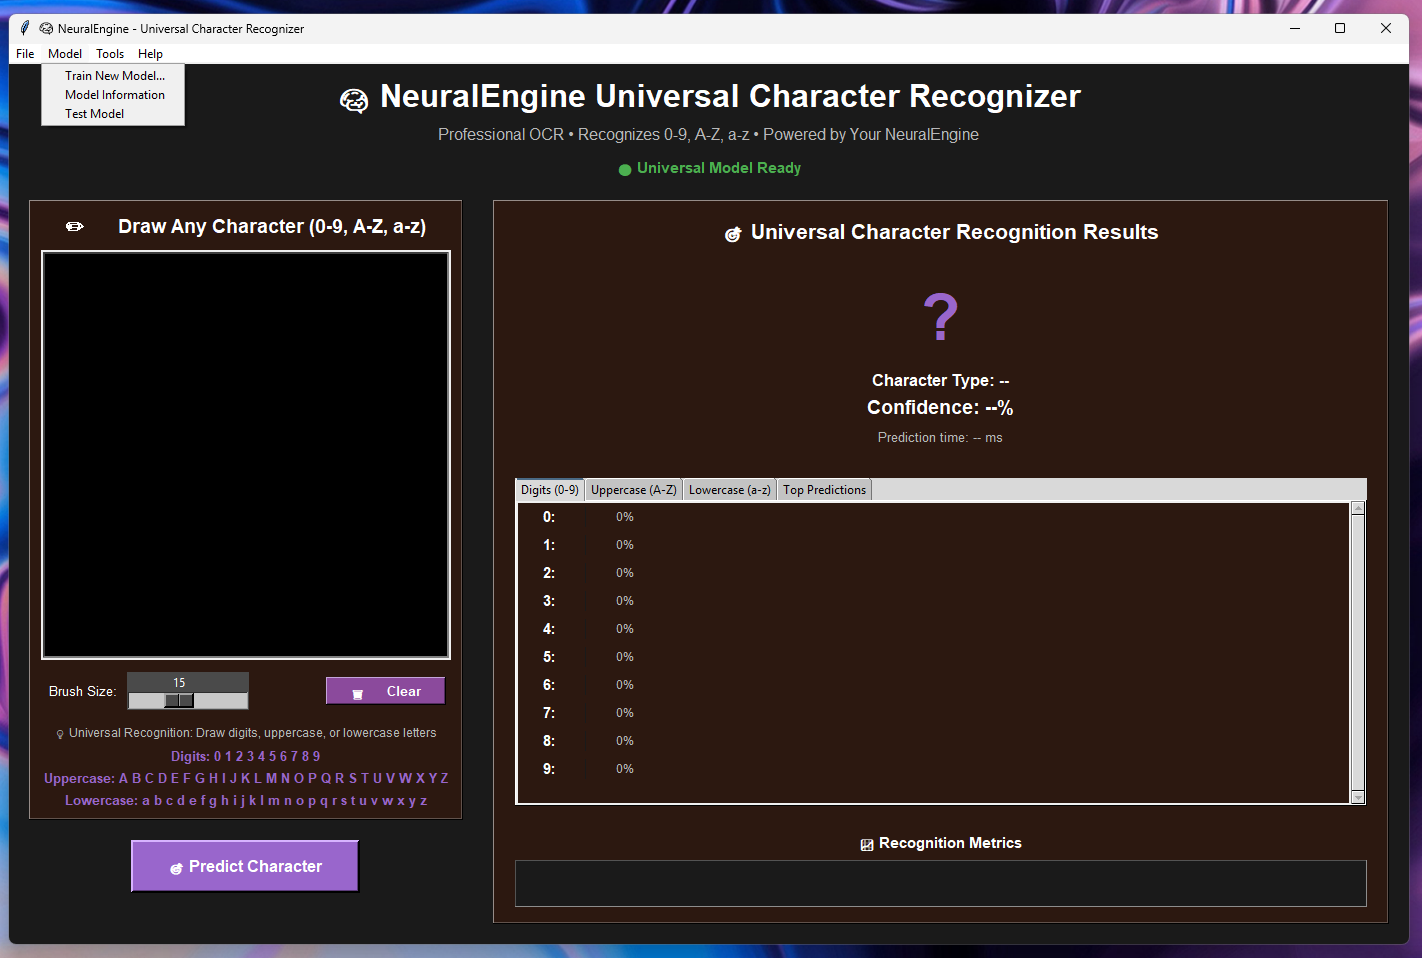
\includegraphics[width=\textwidth]{universal_character_recognizer_interface.png}
\caption{Universal Character Recognizer Tkinter interface showing the drawing canvas for character input, real-time prediction results across all 62 character classes, confidence scores, and character type classification (digit, uppercase, lowercase) with comprehensive performance statistics.}
\label{fig:universal_interface}
\end{figure}

\subsection{Performance Analysis and Character Type Evaluation}

\subsubsection{Overall Model Performance}

The Universal Character Recognizer achieves 81.45\% test accuracy across all 62 character classes, representing substantial performance considering the complexity of the multi-class recognition task. The model demonstrates 50.5× improvement over random baseline performance (1.61\%), indicating effective learning and feature extraction capabilities.

Training convergence characteristics show stable learning across 150 epochs with total training time of 70.6 minutes. The model achieves 80.0\% average confidence across predictions, suggesting reasonable calibration between prediction confidence and actual accuracy. Test loss of 0.5748 indicates well-controlled overfitting and effective generalization to unseen character samples.

The substantial increase in classification complexity compared to digit recognition naturally impacts overall accuracy, with the 62-class problem presenting inherently greater difficulty than 10-class digit recognition. However, the achieved performance demonstrates the Neural Network Engine's scalability to complex multi-class problems while maintaining reasonable accuracy and confidence characteristics.

\subsubsection{Character Type Performance Analysis}

Detailed analysis reveals significant performance variations across the three character types, reflecting the inherent difficulty differences in recognizing digits, uppercase letters, and lowercase letters:

\textbf{Digit Recognition (0-9)}: Achieves the highest performance with 92.6\% accuracy and 86.1\% average confidence. This superior performance reflects the distinct visual characteristics of digits and the model's ability to leverage patterns learned from extensive digit recognition training. The high confidence scores indicate strong model certainty when classifying numerical characters.

\textbf{Uppercase Letter Recognition (A-Z)}: Demonstrates moderate performance with 75.1\% accuracy and 71.4\% average confidence. Uppercase letters present intermediate difficulty due to their generally distinct shapes while still exhibiting some inter-character similarity (e.g., 'C' and 'G', 'P' and 'R'). The moderate confidence levels reflect the increased uncertainty in distinguishing between similar uppercase characters.

\textbf{Lowercase Letter Recognition (a-z)}: Shows the most challenging performance with 64.9\% accuracy but interestingly higher confidence at 77.1\%. The lower accuracy reflects the significant visual similarity between many lowercase characters and their generally smaller distinguishing features. The higher confidence suggests the model may be overconfident in lowercase predictions, indicating potential calibration issues for this character type.

\begin{figure}[H]
\centering
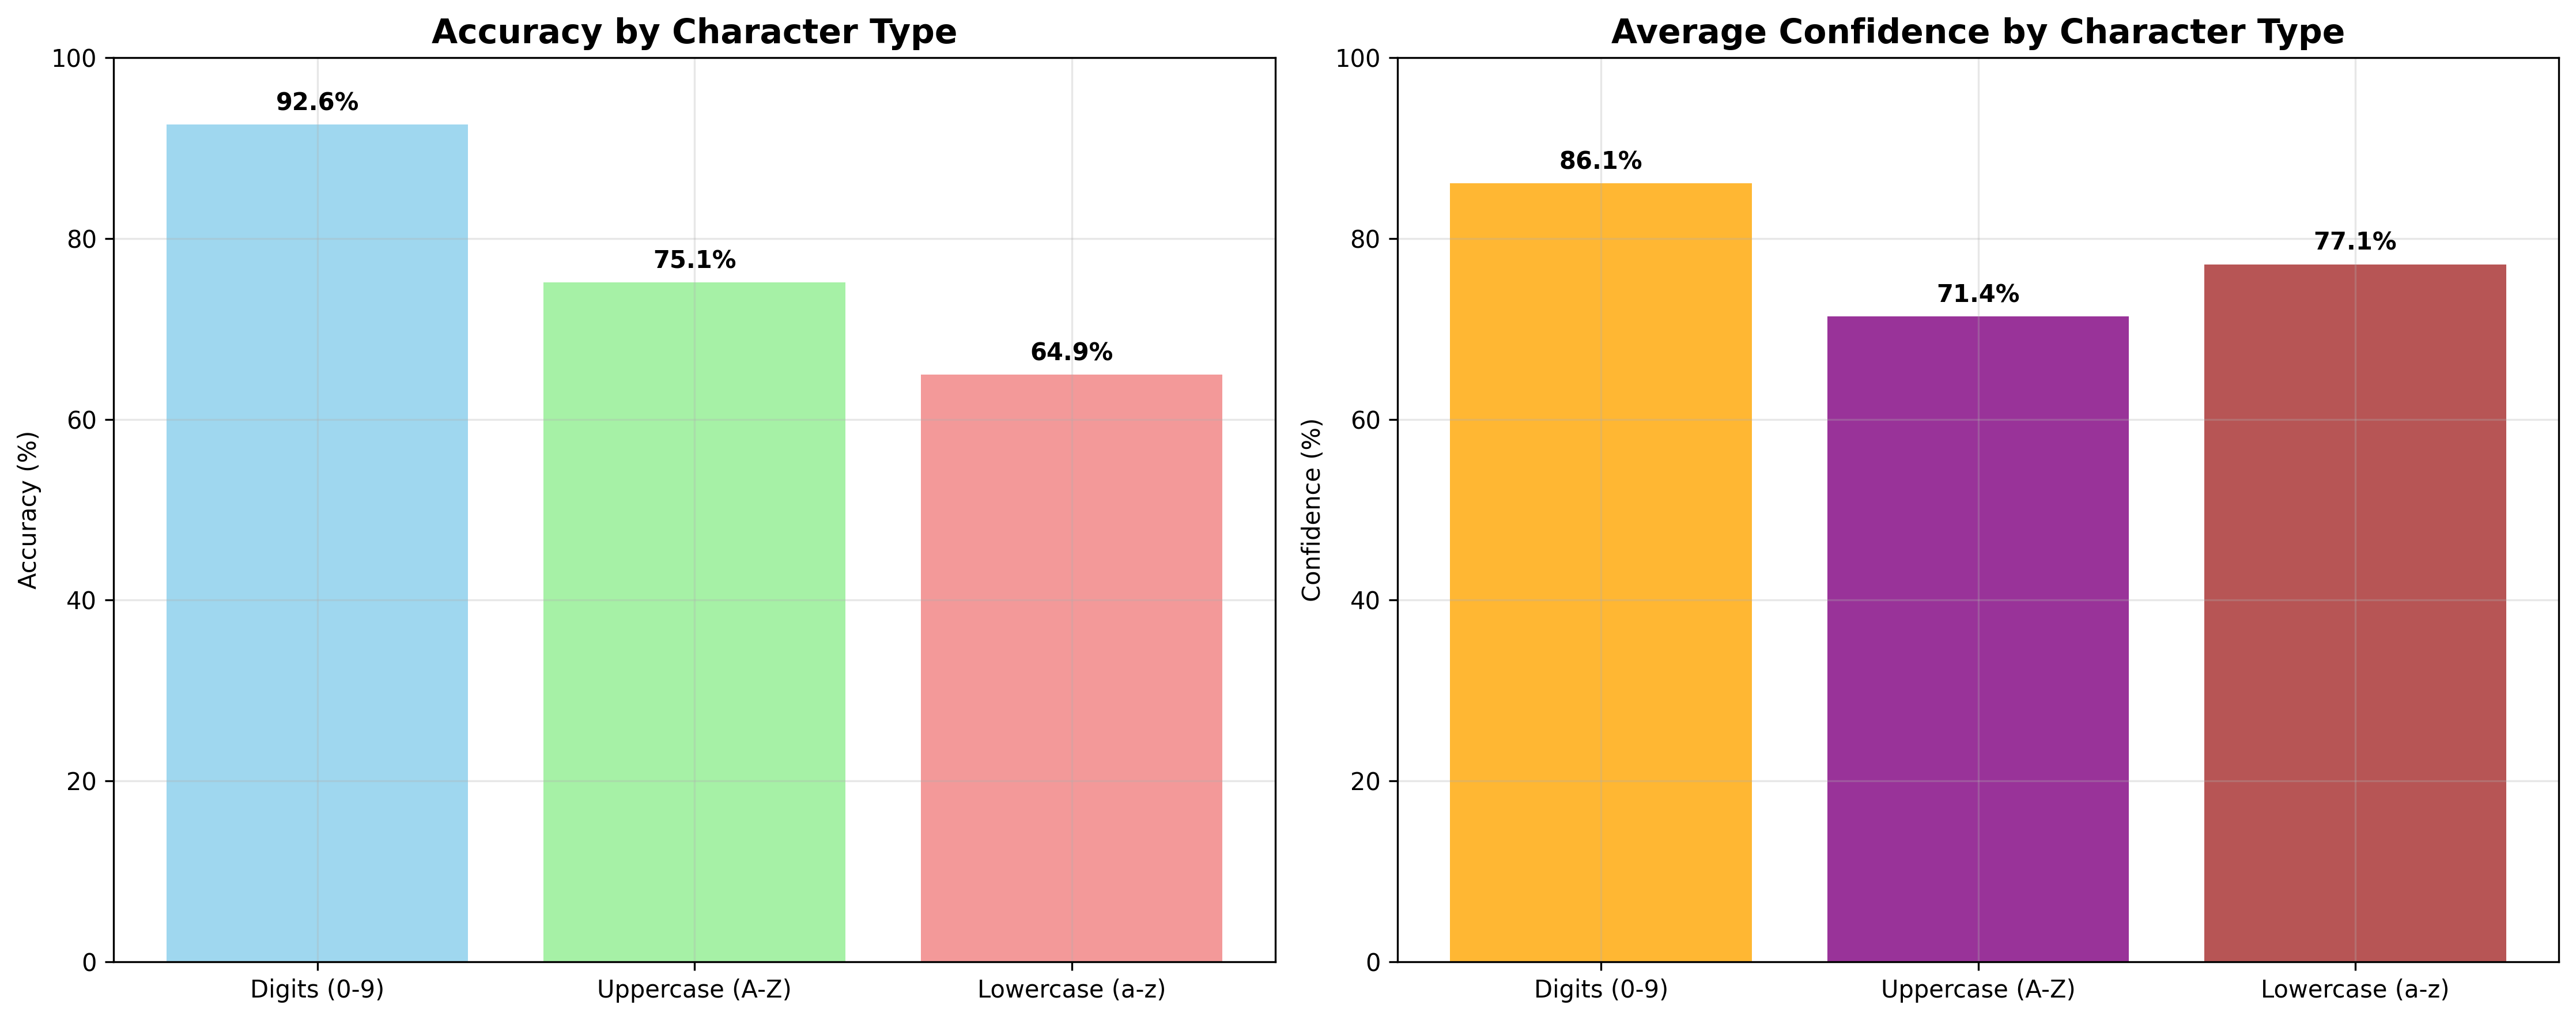
\includegraphics[width=\textwidth]{character_type_performance.png}
\caption{Character type performance analysis showing accuracy and confidence metrics for digits, uppercase letters, and lowercase letters. The visualization demonstrates the performance hierarchy with digits achieving highest accuracy, followed by uppercase letters, while lowercase letters present the greatest recognition challenges despite showing high confidence levels.}
\label{fig:character_type_performance}
\end{figure}

\subsubsection{Detailed Character-Level Performance Analysis}

Character-level analysis reveals specific patterns and challenges within the universal recognition task. The 20 worst-performing characters provide insights into the fundamental difficulties of multi-class character recognition:

\textbf{Lowercase Letter Challenges}: 18 of the 20 worst-performing characters are lowercase letters, highlighting the inherent difficulty in distinguishing between similar lowercase character shapes. Characters like 'o', 's', 'c', and 'u' show particularly poor performance due to their rounded shapes and similar stroke patterns that create ambiguity in recognition.

\textbf{Visual Similarity Issues}: Characters with similar visual appearance across different cases (e.g., 'O' vs 'o', 'I' vs 'l') consistently show reduced performance. The model struggles to learn subtle differences that distinguish these visually similar characters, particularly when stroke width and character positioning variations are considered.

\textbf{Sample Distribution Impact}: Some poorly performing characters have limited training samples, suggesting that class imbalance affects model performance. Characters with fewer training examples show reduced accuracy, indicating the importance of balanced training data for optimal multi-class performance.

\begin{figure}[H]
\centering
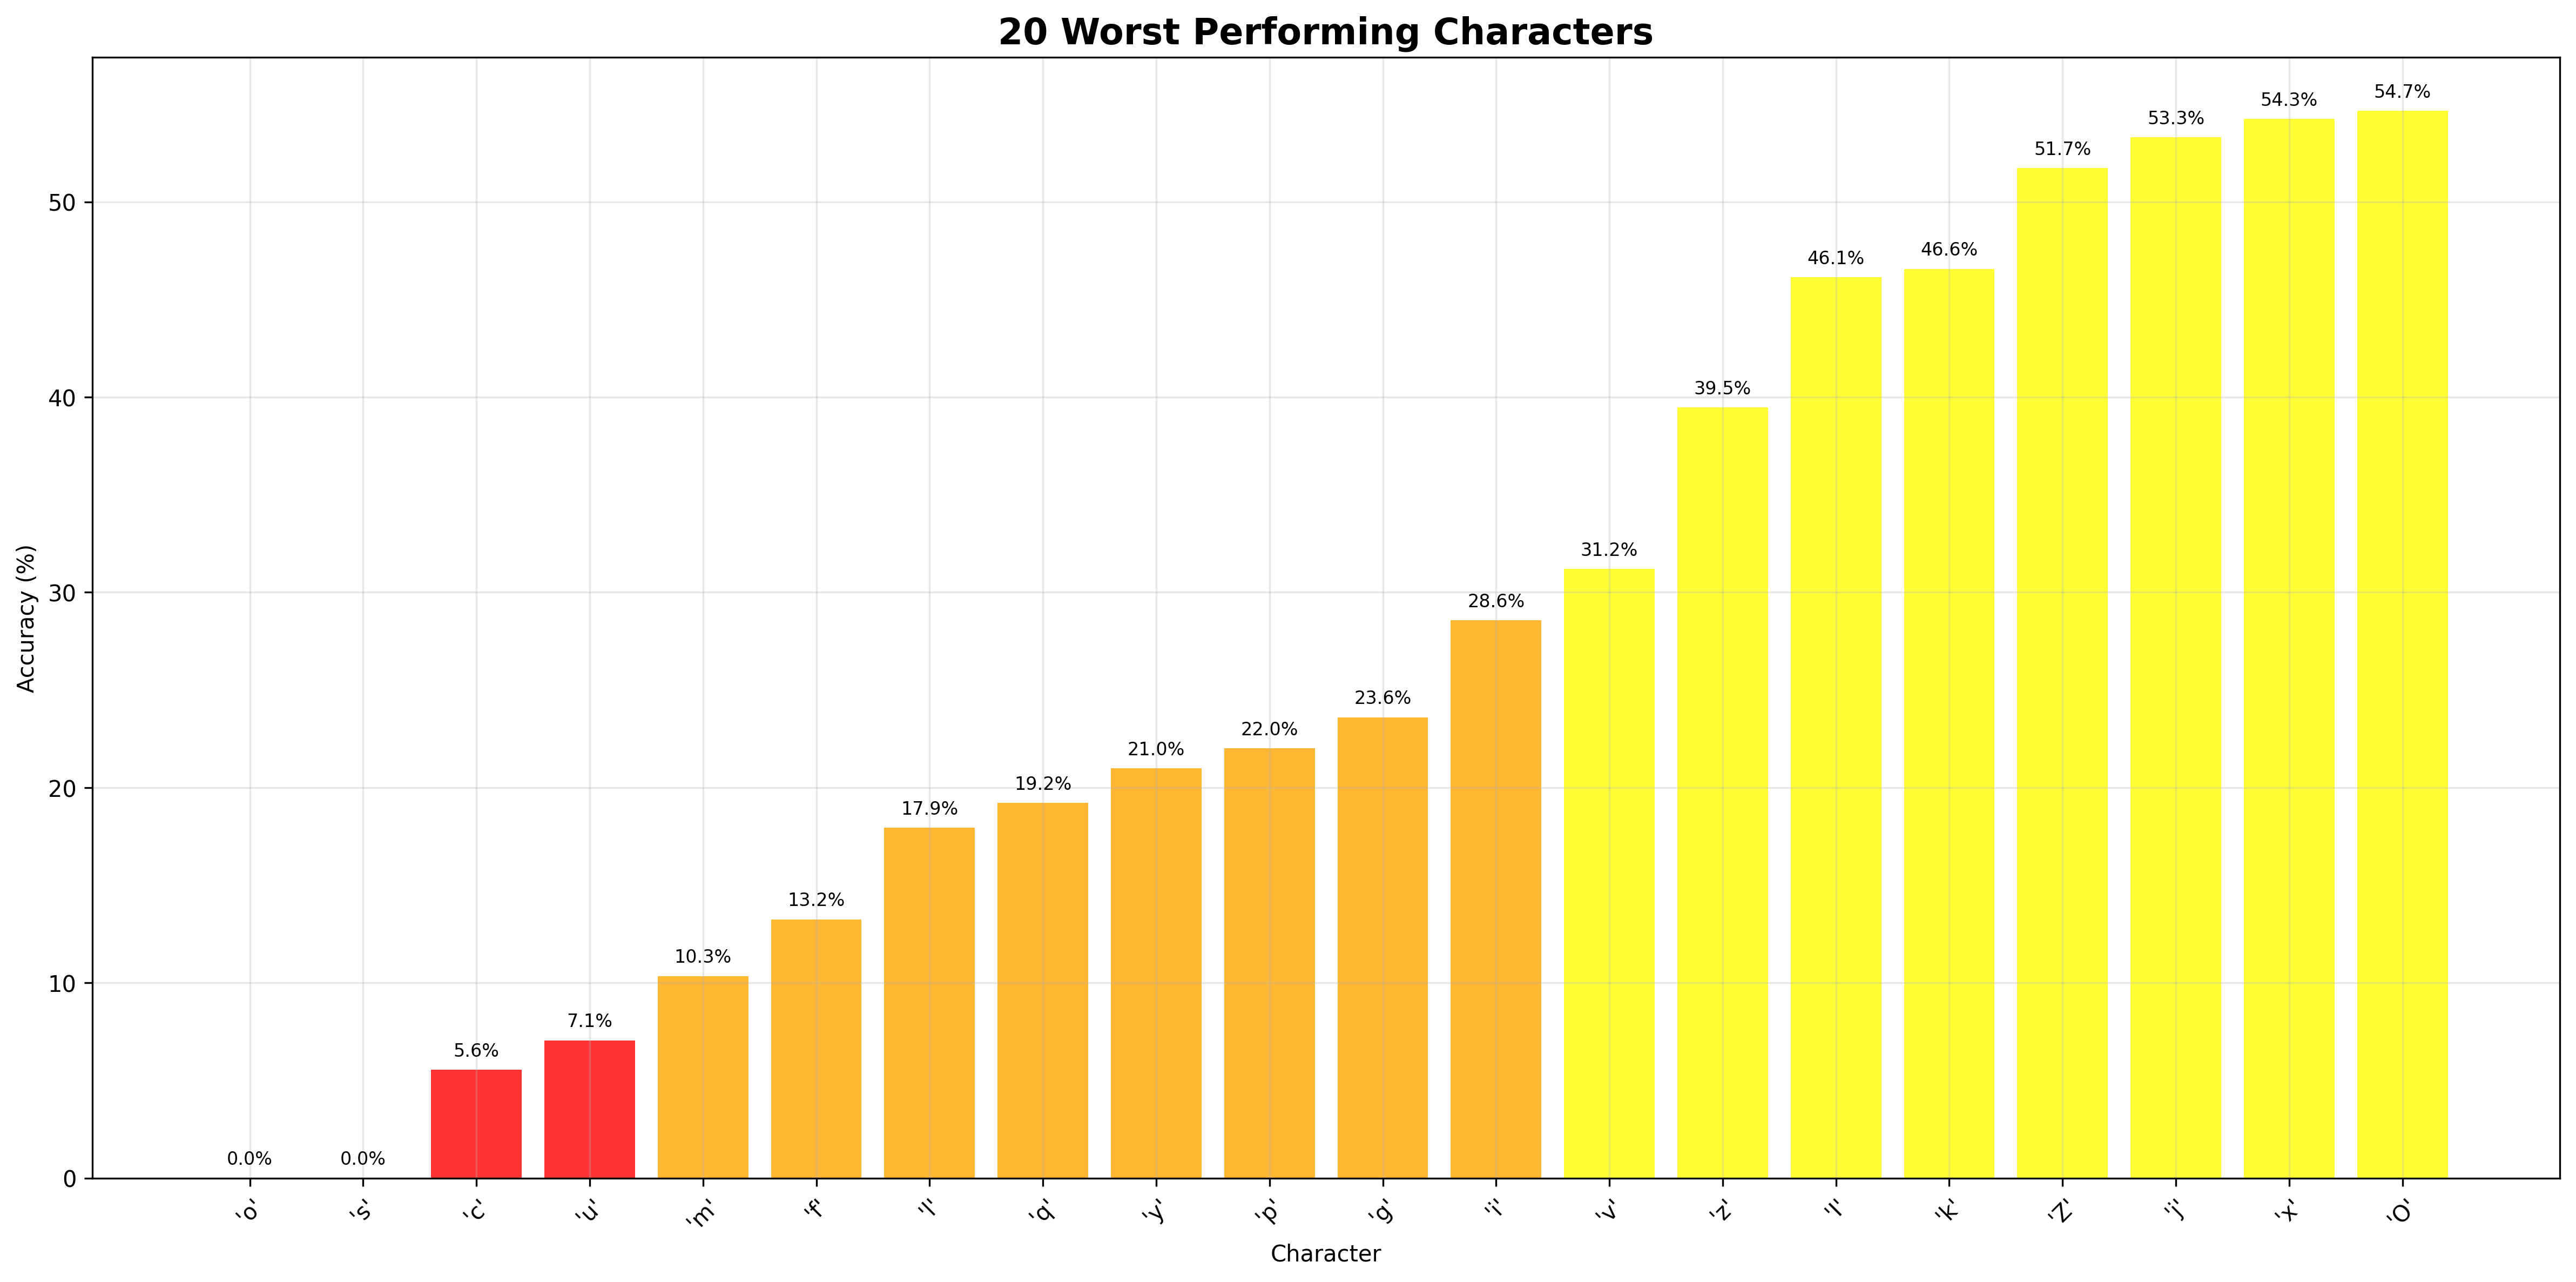
\includegraphics[width=\textwidth]{worst_characters.png}
\caption{Analysis of the 20 worst-performing characters in universal character recognition, showing predominantly lowercase letters with accuracy ranging from 0\% to 54.7\%. The visualization highlights the specific challenges in lowercase character recognition and provides insights into character-level performance patterns and confidence distributions.}
\label{fig:worst_characters}
\end{figure}

\subsubsection{Confidence Analysis and Prediction Reliability}

Comprehensive confidence analysis reveals important characteristics of model prediction reliability across the 62-class recognition task. The overall 80.0\% average confidence provides reasonable correlation with the 81.45\% accuracy, suggesting adequate model calibration for practical applications.

\textbf{Confidence Distribution Patterns}: Analysis shows that confidence levels vary significantly across character types and individual characters. Digits consistently show higher confidence scores corresponding to their higher accuracy rates. Uppercase letters demonstrate moderate confidence alignment with accuracy, while lowercase letters exhibit confidence-accuracy misalignment suggesting potential overconfidence issues.

\textbf{Correct vs Incorrect Prediction Confidence}: Examination of confidence patterns for correct versus incorrect predictions reveals important model behavior characteristics. Correctly classified characters generally show higher confidence scores, while misclassified characters often exhibit lower confidence, providing potential mechanisms for prediction reliability assessment.

\textbf{Practical Implications}: The confidence analysis suggests that prediction confidence can serve as a useful indicator of classification reliability, particularly for applications requiring high accuracy assurance. Characters with confidence scores below certain thresholds may benefit from alternative recognition strategies or human verification.

\begin{figure}[H]
\centering
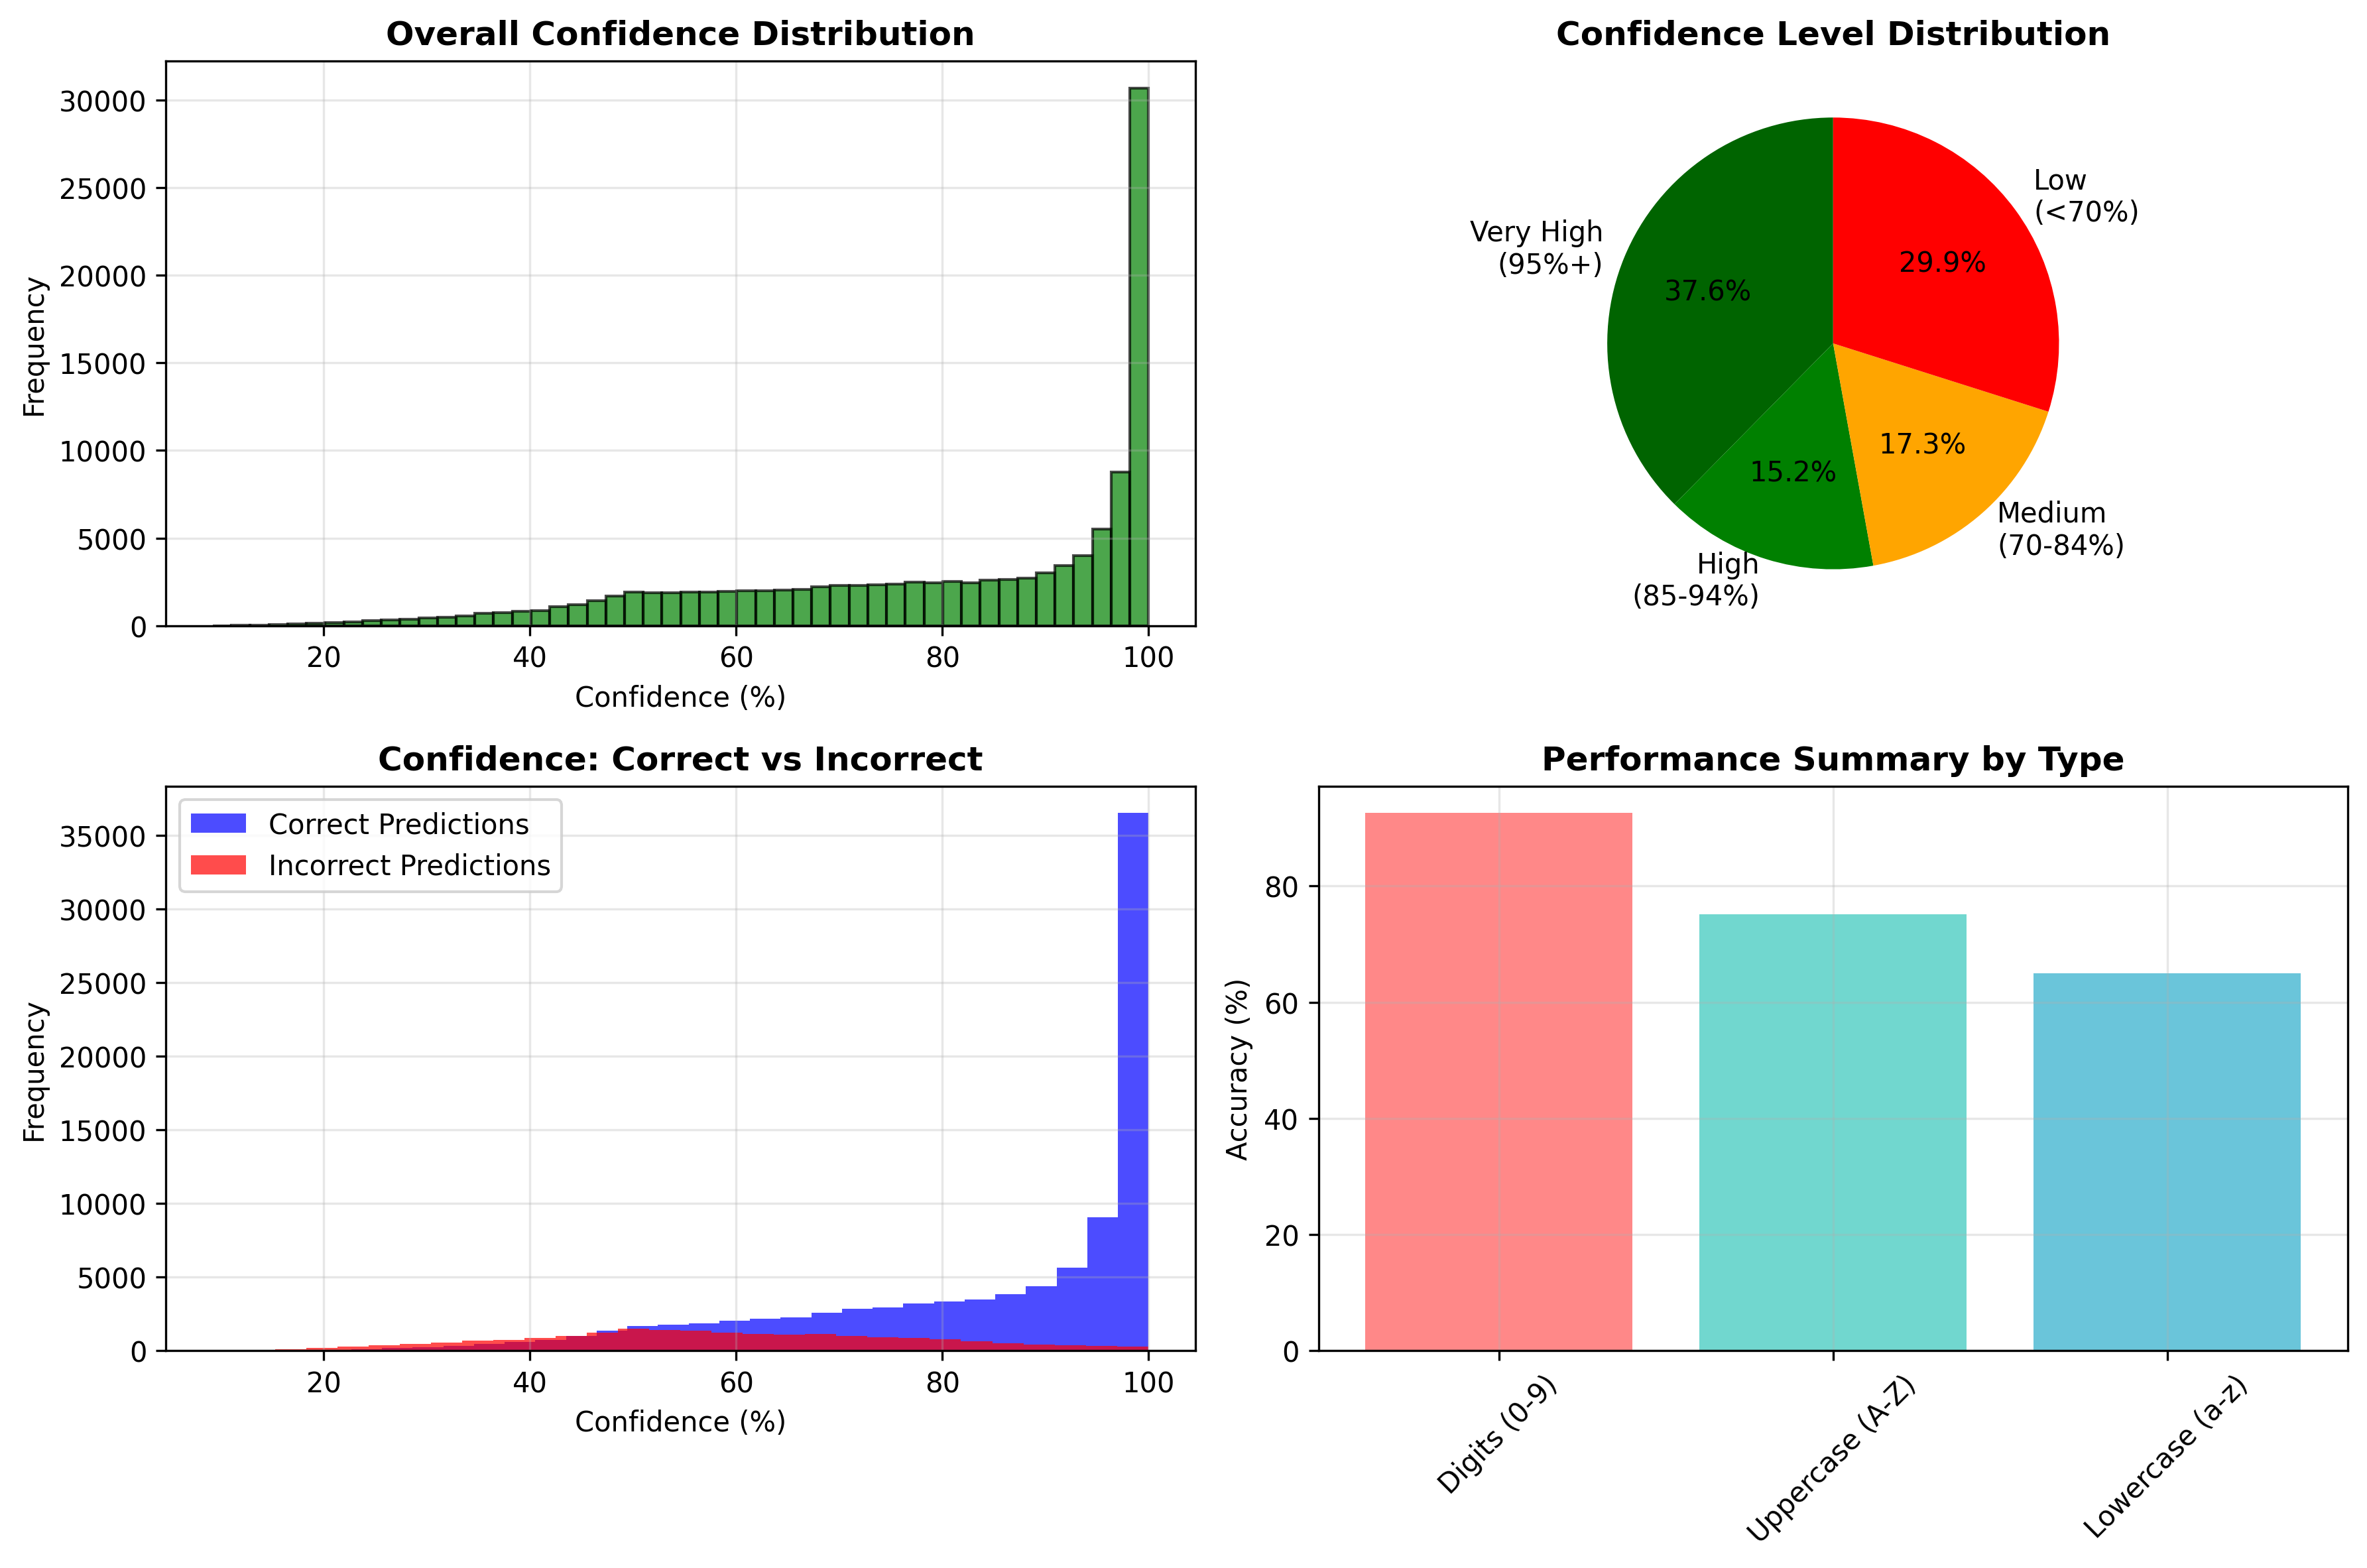
\includegraphics[width=\textwidth]{universal_confidence_analysis.png}
\caption{Comprehensive confidence analysis featuring four analytical perspectives: overall confidence distribution across all predictions, confidence level categorization showing high/medium/low confidence regions, confidence comparison between correct and incorrect predictions, and performance summary statistics by character type demonstrating prediction reliability patterns.}
\label{fig:universal_confidence}
\end{figure}

\subsection{Implementation Challenges and Technical Insights}

\subsubsection{Scaling Challenges in Multi-Class Recognition}

The transition from 10-class digit recognition to 62-class universal character recognition presents several scaling challenges that provide insights into neural network behavior on complex classification tasks:

\textbf{Parameter Scaling}: The increased output dimensionality requires 62 output neurons compared to 10 for digit recognition, resulting in substantial parameter increases in the final layer. This expansion affects both memory requirements and computational complexity during training and inference.

\textbf{Training Stability}: Larger class spaces generally require more careful hyperparameter tuning and training strategies. The multi-phase training approach proves essential for achieving stable convergence across all 62 classes while maintaining reasonable training times.

\textbf{Gradient Flow Complexity}: With 62 output classes, gradient flow patterns become more complex during backpropagation. The softmax function must distribute gradients across a larger probability space, potentially affecting learning dynamics and convergence characteristics.

\subsubsection{Future Improvement Possibilities}

Several approaches could potentially improve universal character recognition performance:

\textbf{Data Augmentation}: Implementing character-specific data augmentation strategies including rotation, scaling, and stroke width variation could improve robustness to character variations and increase effective training data for underrepresented characters.

\textbf{Architecture Optimization}: Exploring alternative architectures including convolutional layers for better spatial feature extraction or attention mechanisms for focusing on distinguishing character features could improve recognition accuracy.

\textbf{Hierarchical Classification}: Implementing hierarchical approaches that first classify character type (digit/uppercase/lowercase) before performing within-type classification could improve overall accuracy by leveraging type-specific feature extraction.

\textbf{Confidence Calibration}: Developing improved confidence calibration techniques, particularly for lowercase letters, could provide better prediction reliability estimates and support more robust decision-making in practical applications.

\textbf{Class Balancing}: Implementing advanced class balancing techniques including focused sampling, loss function weighting, or synthetic data generation could address performance disparities between frequent and rare characters.

\subsection{Performance Visualization and Comparative Analysis}

The Universal Character Recognizer demonstrates the Neural Network Engine's capability to handle complex multi-class recognition tasks while revealing important insights about the challenges inherent in large-scale classification problems. The achieved 81.45\% accuracy represents substantial performance on a challenging 62-class recognition task, with clear performance hierarchies reflecting the inherent difficulty differences between character types.

The detailed character-level analysis provides valuable insights into specific recognition challenges and suggests directions for future optimization. The confidence analysis reveals important model behavior characteristics that support practical deployment considerations and reliability assessment strategies.

\begin{table}[H]
\centering
\caption{Universal Character Recognizer comprehensive performance summary showing overall metrics and detailed breakdown by character type.}
\label{tab:universal_performance}
\begin{tabular}{lccccc}
\toprule
Metric & Overall & Digits (0-9) & Uppercase (A-Z) & Lowercase (a-z) & Baseline \\
\midrule
Accuracy & 81.45\% & 92.6\% & 75.1\% & 64.9\% & 1.61\% \\
Confidence & 80.0\% & 86.1\% & 71.4\% & 77.1\% & N/A \\
Classes & 62 & 10 & 26 & 26 & 62 \\
Samples (Test) & 116,323 & 18,800 & 47,223 & 50,300 & 116,323 \\
Improvement & 50.5× & 57.5× & 46.6× & 40.3× & 1.0× \\
\bottomrule
\end{tabular}
\end{table}

The Universal Character Recognizer successfully demonstrates the Neural Network Engine's scalability from simple 10-class digit recognition to complex 62-class universal character recognition. While the increased complexity naturally impacts overall accuracy compared to specialized digit recognizers, the achieved performance validates the engine's effectiveness for complex multi-class problems. The detailed analysis provides valuable insights into character recognition challenges and establishes a foundation for future optimization efforts in universal character recognition applications.

\section{Quadratic Equations Predictor Web Application}

The Quadratic Equations Predictor Web Application represents the most ambitious and innovative component of the Neural Network Engine ecosystem, demonstrating the framework's capabilities in experimental research domains beyond traditional machine learning applications. This comprehensive web-based platform provides a complete research environment for investigating neural network applications in mathematical problem-solving, specifically focusing on quadratic equation analysis and prediction across multiple mathematical scenarios.

The application transcends conventional neural network applications by exploring the intersection of symbolic mathematics and machine learning, providing researchers and educators with sophisticated tools for generating datasets, training multiple model architectures, and conducting comprehensive performance analysis. The platform's modular design enables systematic investigation of different mathematical prediction scenarios while maintaining rigorous experimental controls and detailed performance tracking.

\subsection{Research Objectives and Motivation}

\subsubsection{Experimental Neural Network Applications}

The Quadratic Equations Predictor addresses a fundamental research question: can neural networks effectively learn mathematical relationships that have well-defined algebraic solutions? While quadratic equations possess closed-form solutions through the quadratic formula, this application investigates whether neural networks can discover these mathematical relationships through pattern recognition and approximate the solutions with sufficient accuracy for practical applications.

This research direction explores several compelling aspects of machine learning: the ability of neural networks to approximate symbolic mathematical operations, the effectiveness of different architectural approaches for mathematical prediction tasks, the impact of dataset characteristics on mathematical learning, and the potential for neural networks to generalize mathematical concepts beyond their training distribution.

The experimental framework provides insights into fundamental questions about neural network capabilities in mathematical domains, including convergence characteristics for well-defined mathematical problems, generalization performance across different coefficient ranges, robustness to numerical precision requirements, and the relationship between network architecture and mathematical accuracy.

\subsubsection{Research Methodology and Goals}

The research methodology employs a systematic approach to investigating neural network performance across five distinct mathematical scenarios, each representing different aspects of quadratic equation analysis. This multi-scenario approach enables comprehensive evaluation of neural network capabilities while providing practical insights into the most effective applications of machine learning in mathematical contexts.

Primary research objectives include: establishing baseline performance metrics for mathematical prediction tasks, identifying optimal network architectures for different mathematical scenarios, analyzing the relationship between dataset characteristics and model performance, developing systematic approaches for mathematical dataset generation, and creating comprehensive evaluation frameworks for mathematical machine learning applications.

The platform enables controlled experimentation through standardized dataset generation, consistent training methodologies, systematic performance evaluation, and comparative analysis across multiple model architectures. This rigorous approach ensures reproducible results and meaningful insights into neural network behavior in mathematical domains.

\begin{figure}[H]
\centering
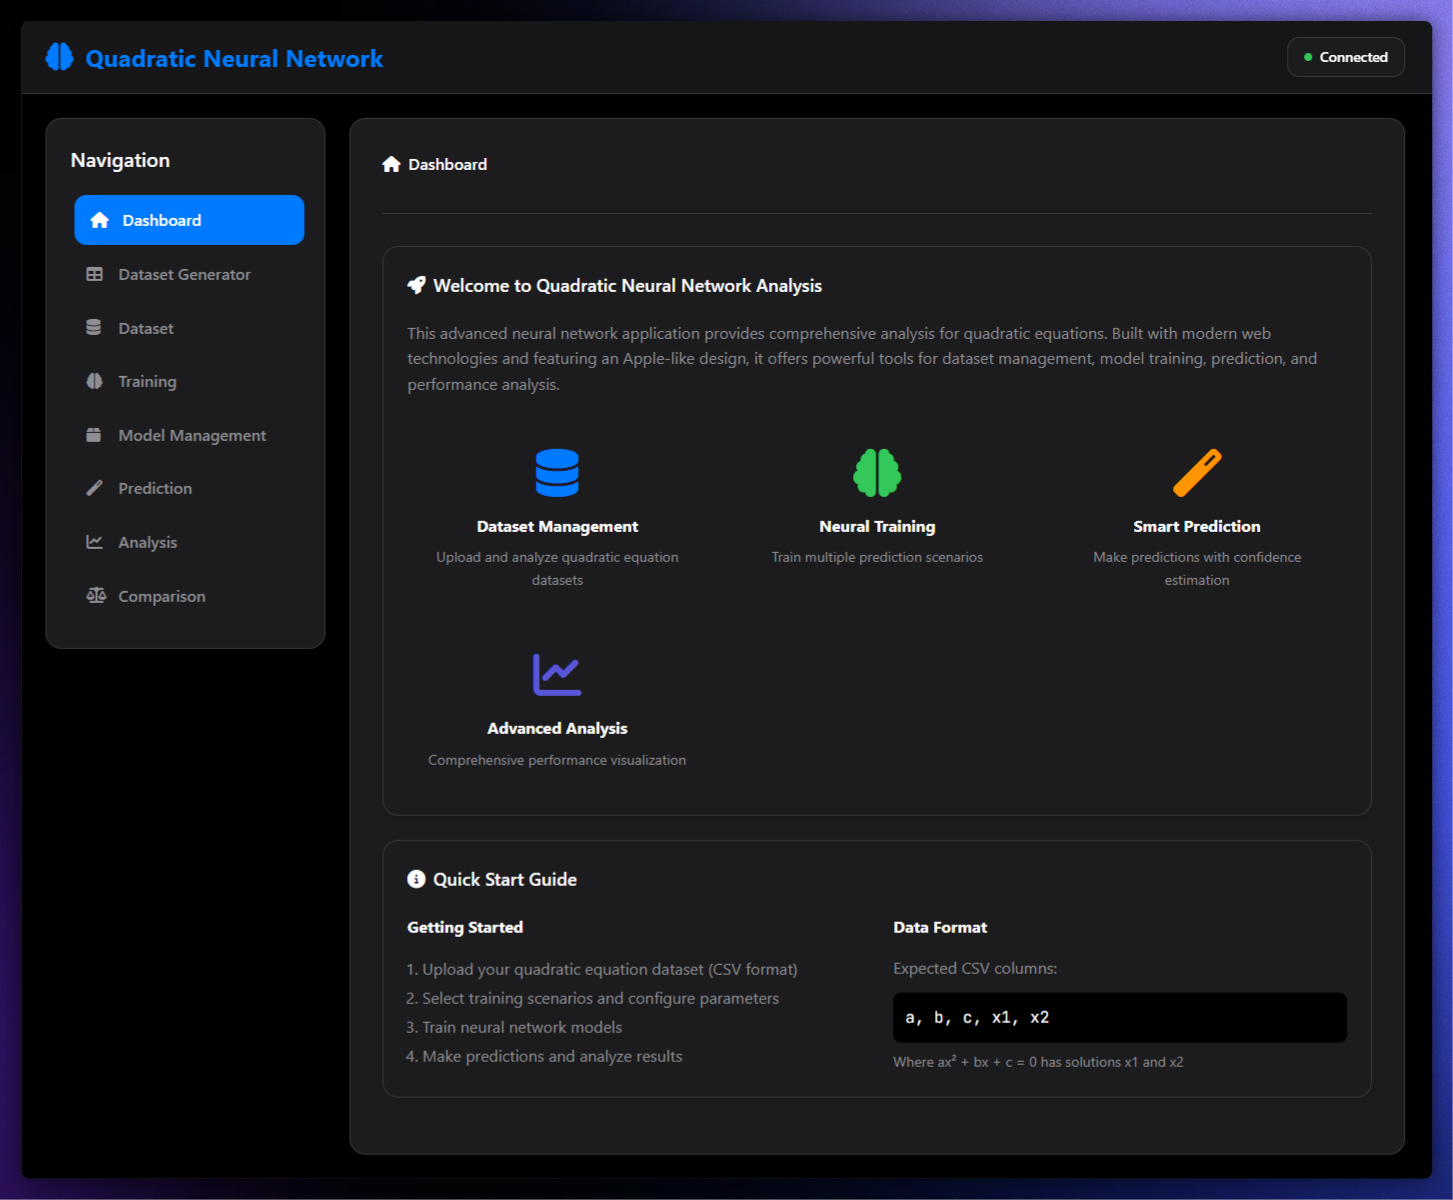
\includegraphics[width=\textwidth]{quadratic_predictor_dashboard.png}
\caption{Quadratic Equations Predictor dashboard providing comprehensive overview of the research platform, quick start guide, and navigation to all major functional areas including dataset generation, model training, and analysis tools.}
\label{fig:quadratic_dashboard}
\end{figure}

\subsection{Web Application Features}

\subsubsection{Advanced Dataset Generation Capabilities}

The Dataset Generator represents the cornerstone of the research platform, providing sophisticated tools for creating mathematically rigorous and educationally relevant quadratic equation datasets. The generator implements multiple generation modes designed to address different research objectives and educational contexts.

\textbf{Integer Solutions Mode} generates quadratic equations guaranteed to have integer roots, eliminating floating-point precision issues and providing clean mathematical relationships ideal for initial neural network training. This mode ensures that all generated equations produce whole number solutions, facilitating easier interpretation of results and reducing numerical complexity during training.

\textbf{Fractional Solutions Mode} expands the mathematical complexity by including equations with rational root solutions, introducing controlled numerical precision challenges that reflect real-world mathematical applications. This mode enables investigation of neural network performance with more complex mathematical relationships while maintaining mathematical validity.

\textbf{School Grade Mode} implements a specialized generation algorithm that creates equations matching patterns commonly found in educational textbooks and standardized assessments. This mode utilizes specific coefficient distributions and mathematical structures that align with pedagogical standards, ensuring educational relevance and practical applicability.

\textbf{Perfect Square Discriminant Mode} generates equations with discriminants that are perfect squares, ensuring clean radical expressions in analytical solutions. This mode facilitates accurate comparison between neural network predictions and exact mathematical solutions while eliminating irrational number complications.

The generator provides comprehensive control over equation characteristics including coefficient ranges with user-specified minimum and maximum values, sample size specification supporting generation of millions of equations for large-scale training, coefficient distribution patterns ensuring mathematical diversity, and solution complexity levels matching specific research objectives.

\textbf{Infinite Generation Mode} provides continuous equation generation with progressively expanding coefficient ranges, enabling investigation of neural network performance across increasing mathematical complexity. This mode supports long-term training experiments and analysis of model performance degradation with increasing problem difficulty.

\begin{figure}[H]
\centering
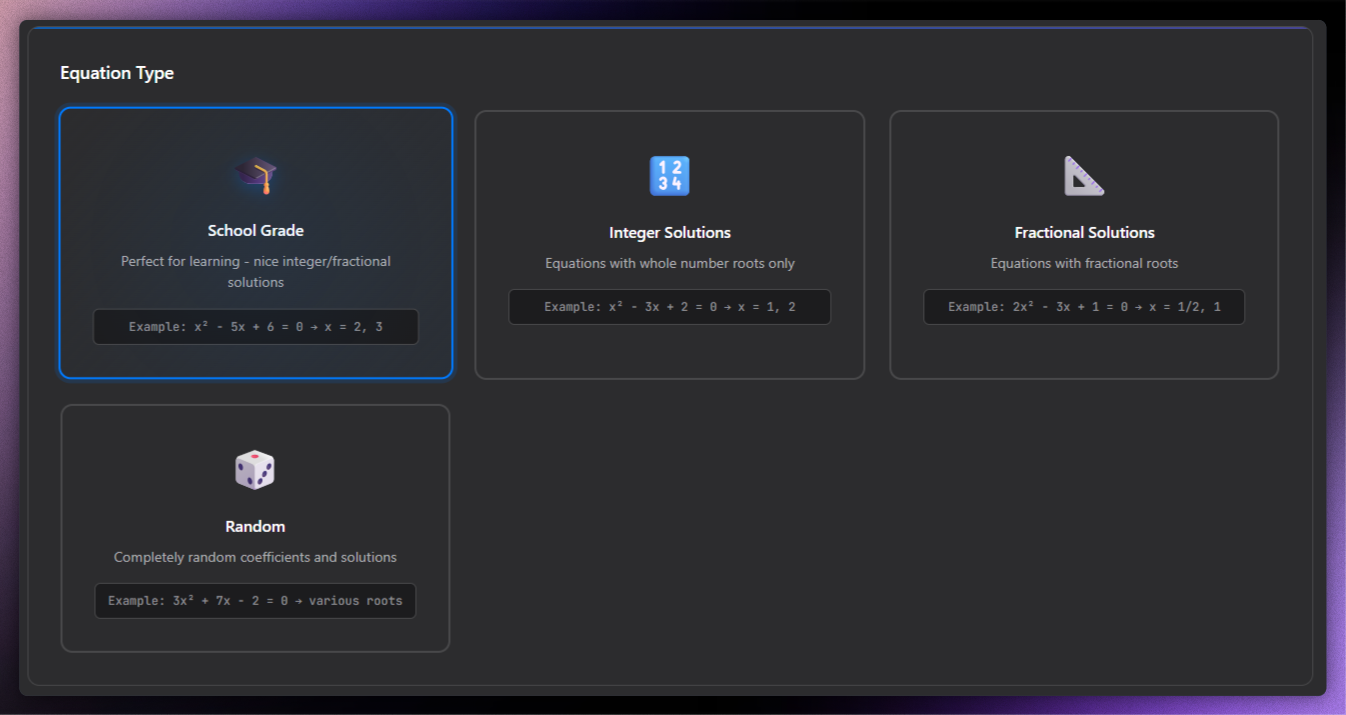
\includegraphics[width=\textwidth]{quadratic_predictor_generation_modes.png}
\caption{Dataset Generator modes interface displaying the five generation modes with their respective mathematical characteristics, coefficient control options, and solution type specifications for creating targeted quadratic equation datasets.}
\label{fig:quadratic_generation_modes}
\end{figure}

\begin{figure}[H]
\centering
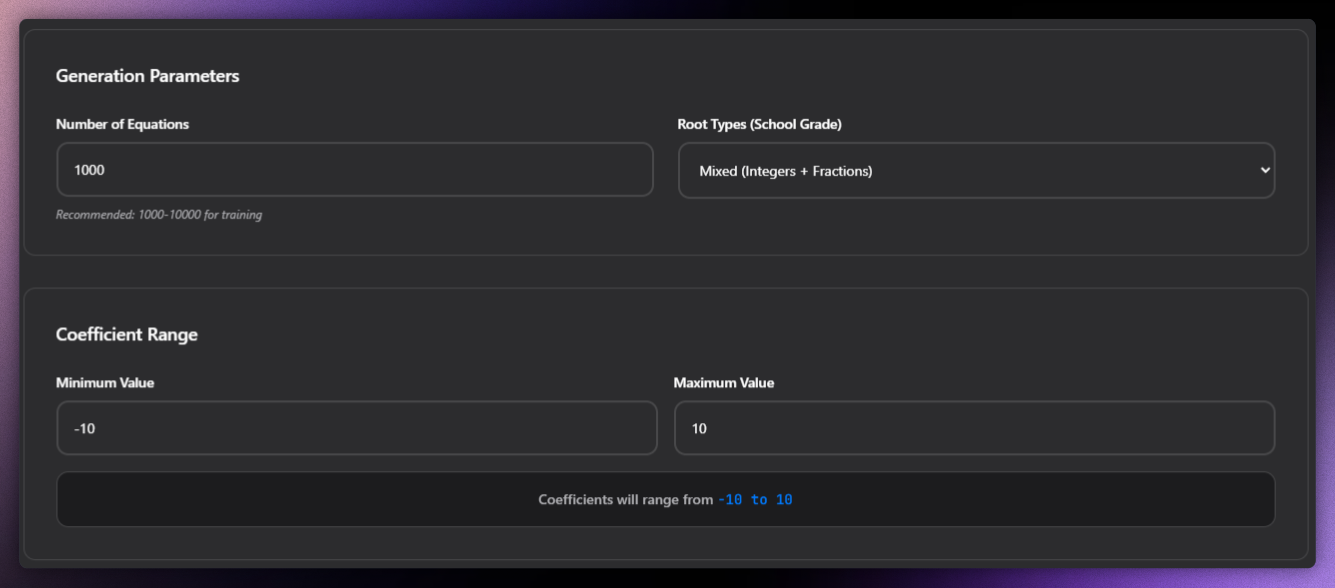
\includegraphics[width=\textwidth]{quadratic_predictor_generator_config.png}
\caption{Dataset Generator configuration options showing comprehensive parameter controls including coefficient ranges, sample size specifications, mathematical constraints, and real-time validation of generation parameters for optimal dataset creation.}
\label{fig:quadratic_generator_config}
\end{figure}

\begin{figure}[H]
\centering
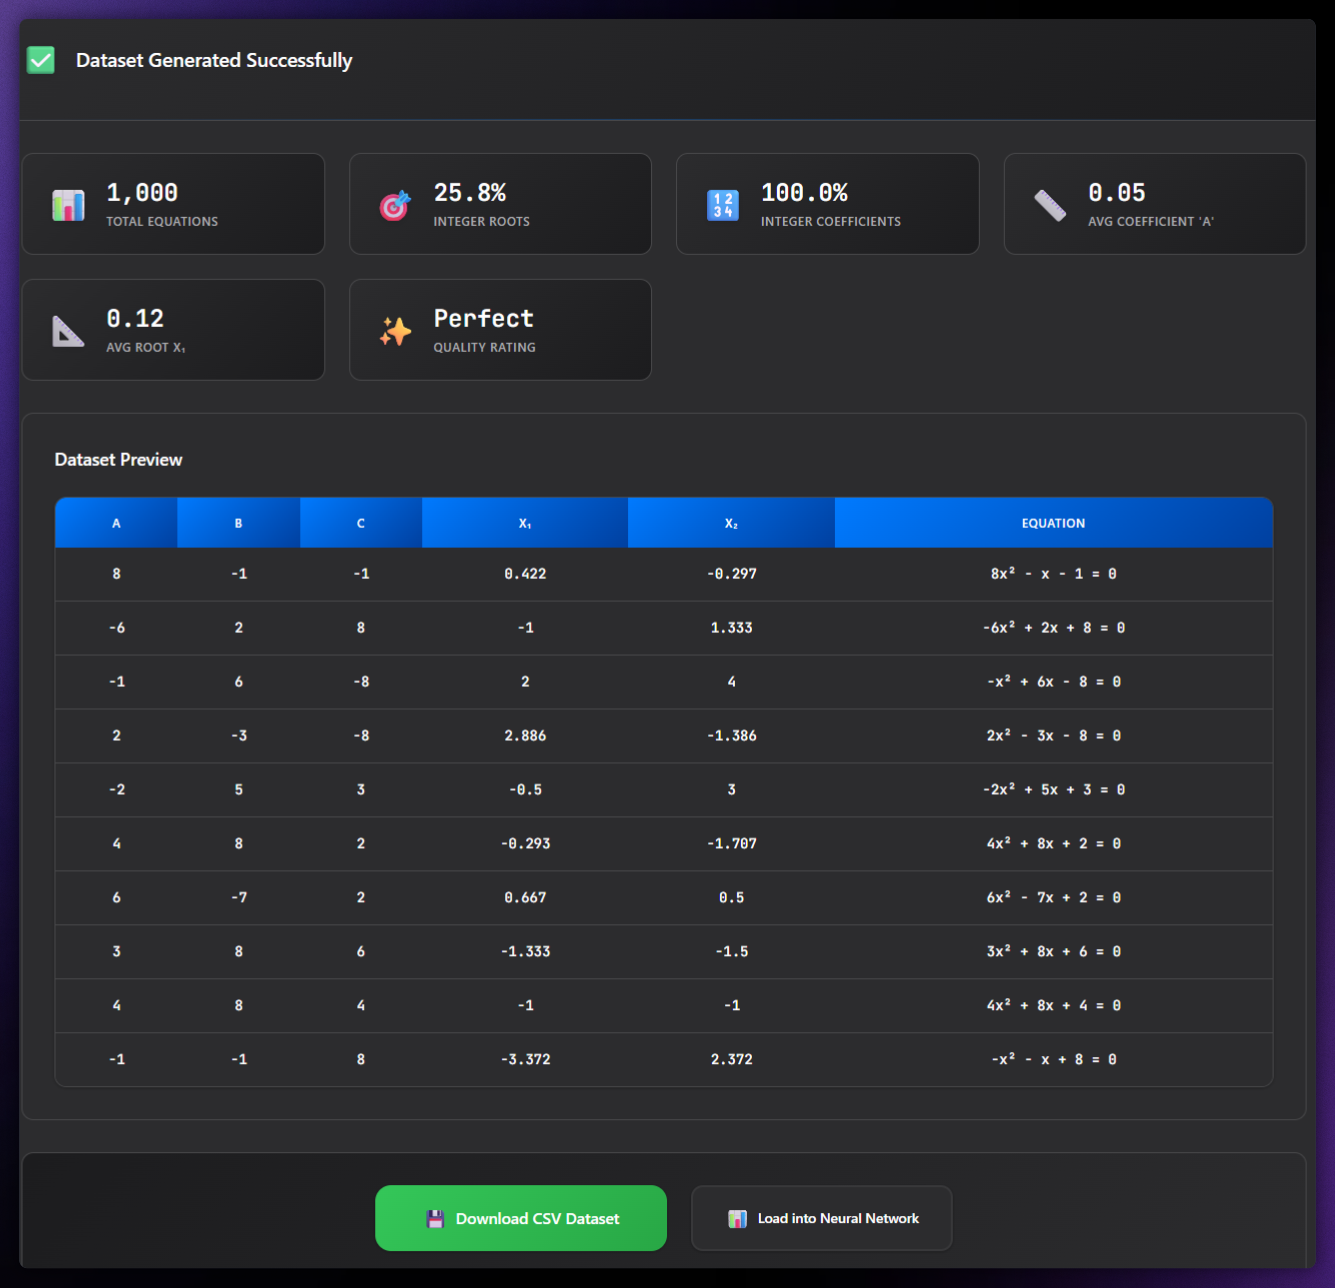
\includegraphics[width=\textwidth]{quadratic_predictor_dataset_preview.png}
\caption{Dataset preview, CSV export, and neural network integration interface displaying generated equation samples, statistical analysis, data quality metrics, and one-click integration options for immediate model training.}
\label{fig:quadratic_dataset_preview}
\end{figure}

\subsubsection{Comprehensive Dataset Management}

The Dataset Management system provides robust capabilities for loading, analyzing, and preprocessing mathematical datasets from various sources. The system supports standard CSV format imports while implementing intelligent data validation and preprocessing specific to mathematical equation datasets.

Dataset preview functionality provides immediate visualization of loaded equations including coefficient distributions, solution characteristics, mathematical complexity metrics, and data quality assessments. Statistical analysis includes coefficient correlation analysis, solution distribution patterns, numerical precision requirements, and dataset balance evaluation across different equation types.

The system implements automatic data validation ensuring mathematical consistency, checking for invalid equations, verifying solution accuracy, and identifying potential numerical precision issues. Quality control measures include outlier detection for extreme coefficient values, solution validation against analytical calculations, and consistency checks across equation parameters.

\begin{figure}[H]
\centering
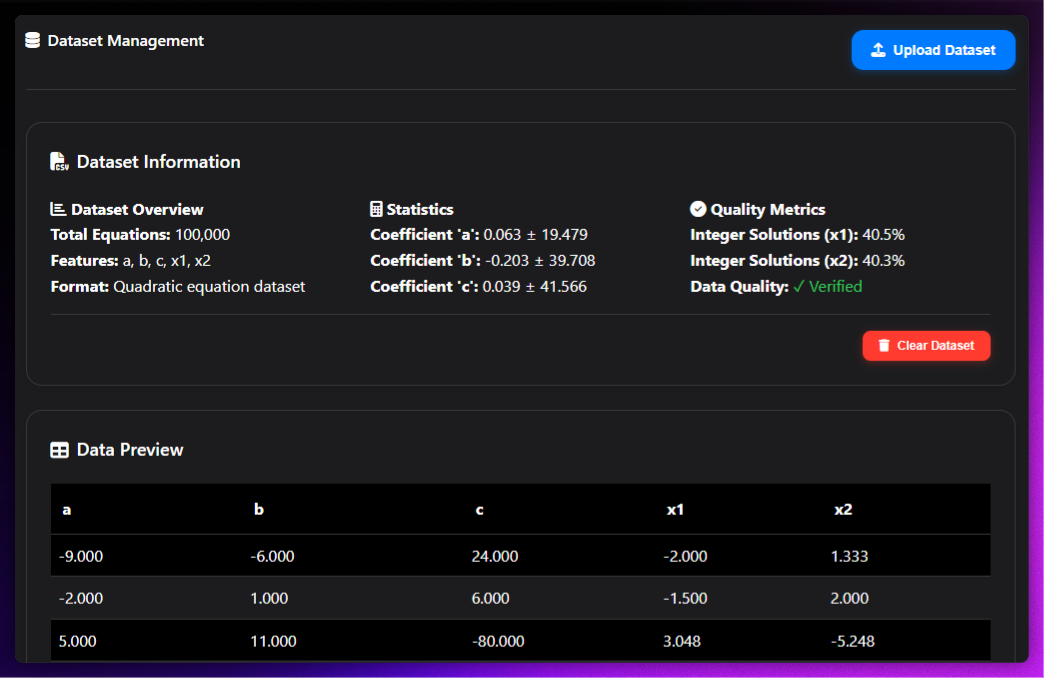
\includegraphics[width=\textwidth]{quadratic_predictor_dataset_tab.png}
\caption{Dataset management interface displaying loaded quadratic equation dataset with comprehensive statistics, coefficient distribution analysis, solution characteristics, and data quality metrics essential for effective neural network training.}
\label{fig:quadratic_dataset}
\end{figure}

\subsubsection{Multi-Scenario Training Framework}

The Training Framework implements a sophisticated multi-scenario approach that investigates neural network performance across five distinct mathematical prediction tasks, each representing different aspects of quadratic equation analysis and practical mathematical applications.

\textbf{Scenario 1: Coefficients to Roots Prediction} represents the most direct application, where neural networks learn to predict solution values (x1, x2) given equation coefficients (a, b, c). This scenario directly parallels the quadratic formula application and provides baseline performance metrics for mathematical prediction accuracy.

\textbf{Scenario 2: Partial Coefficients to Missing Parameters} investigates neural network ability to complete mathematical relationships by predicting missing coefficient (c) and root (x2) given partial information (a, b, x1). This scenario explores interpolation and mathematical relationship learning capabilities.

\textbf{Scenario 3: Roots to Coefficients Prediction} reverses the traditional problem by requiring neural networks to predict equation coefficients (a, b, c) given known solutions (x1, x2). This inverse problem tests the network's understanding of the mathematical relationship from a different perspective.

\textbf{Scenario 4: Single Missing Parameter Prediction} focuses on completing mathematical relationships by predicting the second root (x2) given complete equation information (a, b, c, x1). This scenario tests precision and consistency in mathematical prediction tasks.

\textbf{Scenario 5: Equation Verification} implements a mathematical validity assessment task where neural networks predict the error magnitude given all equation parameters (a, b, c, x1, x2). This scenario explores the network's ability to assess mathematical consistency and identify equation validity.

Each scenario supports independent hyperparameter configuration including epoch specification, learning rate optimization, batch size selection, and optimizer choice. The training framework implements comprehensive logging and monitoring including real-time loss tracking, accuracy metrics evolution, gradient analysis, and convergence diagnostics.

\begin{figure}[H]
\centering
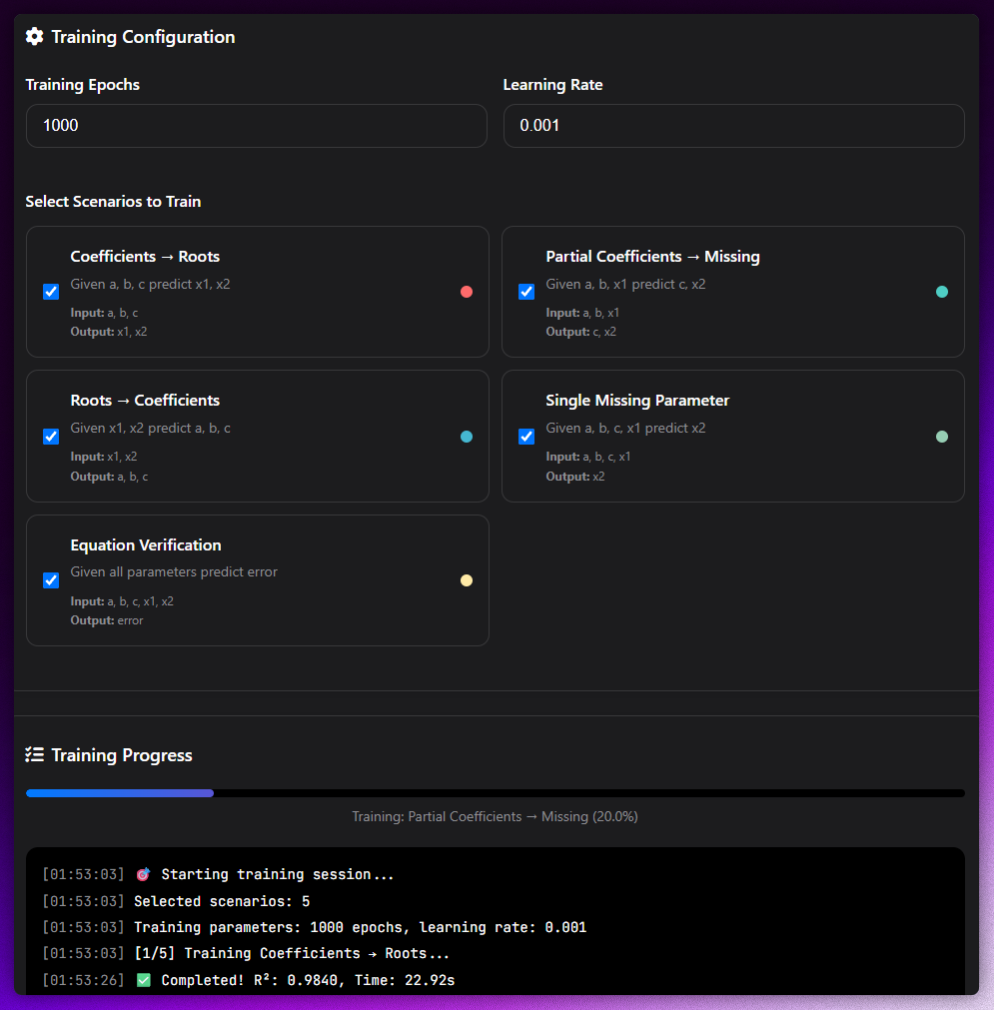
\includegraphics[width=\textwidth]{quadratic_predictor_training_tab.png}
\caption{Multi-scenario training interface enabling simultaneous training of five different neural network approaches to quadratic equation analysis, with independent hyperparameter control, real-time training monitoring, and comprehensive performance tracking across all mathematical prediction scenarios.}
\label{fig:quadratic_training}
\end{figure}

\subsubsection{Advanced Model Management System}

The Model Management system provides enterprise-level capabilities for organizing, storing, and retrieving trained neural network models across all mathematical scenarios. The system implements both individual model management and batch operations for efficient handling of multiple related models.

Individual model saving enables precise control over model storage with user-specified names, detailed metadata preservation, performance metric recording, and training configuration documentation. Each saved model includes comprehensive metadata describing training dataset characteristics, hyperparameter configurations, performance metrics, training duration, and timestamp information.

Batch saving functionality enables simultaneous storage of all trained scenario models with unified naming conventions, organized folder structures, prefix-based naming systems, and collective metadata management. This feature facilitates systematic model organization and supports research workflows requiring comprehensive model version control.

The model loading interface provides sophisticated browsing and selection capabilities with visual model organization, detailed model inspection, performance comparison tools, and intelligent model recommendation systems. Each model displays comprehensive information including R² score analysis, accuracy assessments, training dataset specifications, computational requirements, and performance status classifications.

Model status assessment implements intelligent evaluation criteria providing automated quality ratings such as "Production Ready," "Good Performance," "Needs Improvement," and "Requires Optimization." These assessments consider multiple performance factors including prediction accuracy, training convergence characteristics, generalization performance, and numerical stability.

\begin{figure}[H]
\centering

\includegraphics[width=\textwidth]{quadratic_predictor_model_save.png}
\caption{Model Management batch save interface enabling simultaneous storage of all trained scenario models with unified naming conventions, organized folder structures, and comprehensive metadata preservation for systematic model organization.}
\label{fig:quadratic_model_save}
\end{figure}

\begin{figure}[H]
\centering
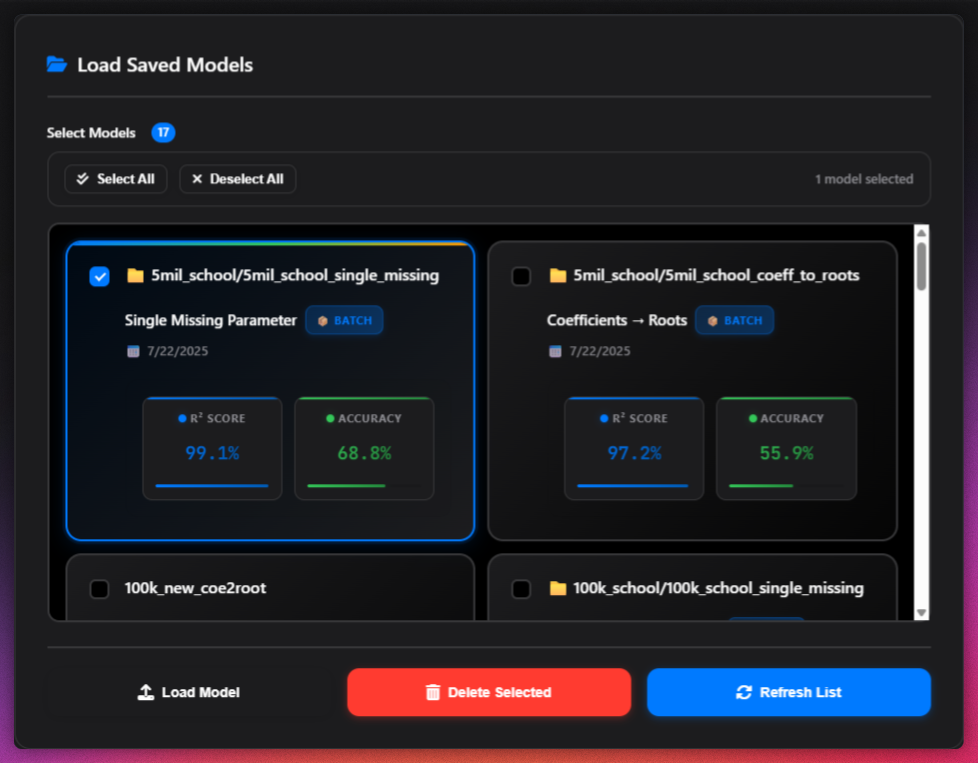
\includegraphics[width=\textwidth]{quadratic_predictor_model_load.png}
\caption{Model loading interface displaying saved model collections with visual organization, detailed model inspection capabilities, performance metrics, and intelligent model selection tools for efficient model retrieval and comparison.}
\label{fig:quadratic_model_load}
\end{figure}

\begin{figure}[H]
\centering
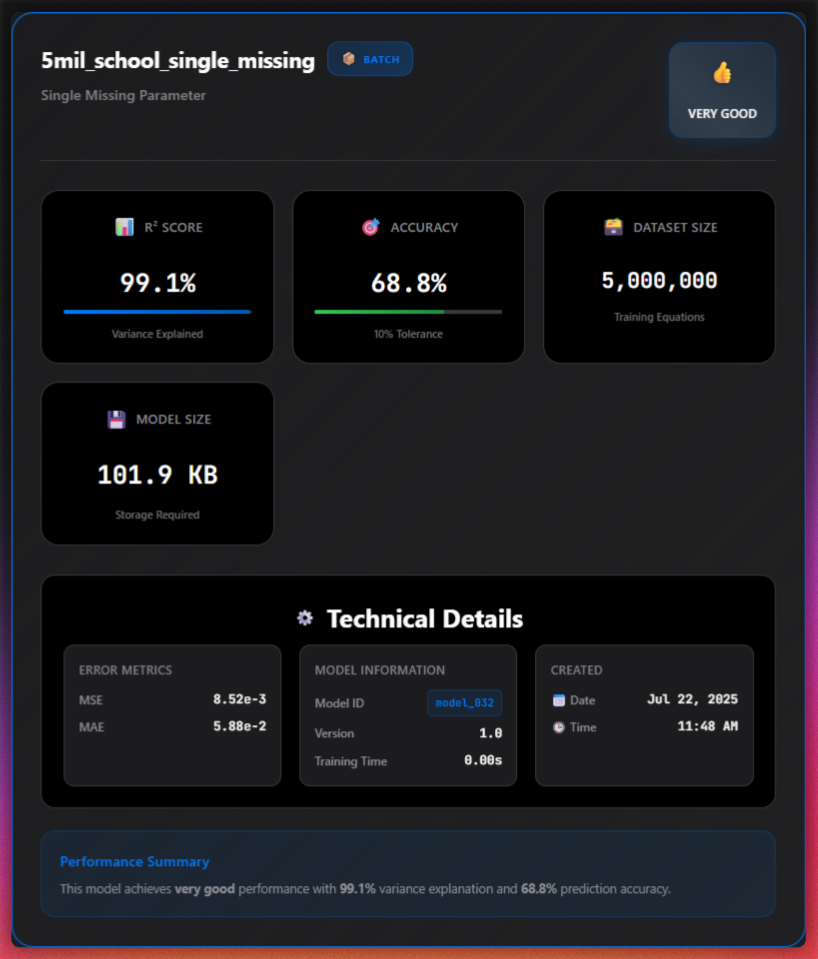
\includegraphics[width=\textwidth]{quadratic_predictor_model_info.png}
\caption{Selected model information panel providing comprehensive model details including R² score analysis, accuracy assessments, training configuration, performance status classification, and metadata for informed model selection decisions.}
\label{fig:quadratic_model_info}
\end{figure}

\subsection{User Interface and Experience}

\subsubsection{Modern Web Design and Interaction Paradigms}

The Quadratic Equations Predictor implements a contemporary web design philosophy emphasizing usability, visual clarity, and efficient workflow management. The interface utilizes modern HTML5, CSS3, and JavaScript technologies to create a responsive, interactive experience that supports both research and educational applications.

The design system implements consistent visual hierarchies with clear navigation patterns, intuitive iconography, responsive layout systems, and accessible interface elements. Color coding systems provide immediate visual feedback for performance metrics, mathematical accuracy, and system status indicators throughout the application.

Interactive elements include real-time data preview, dynamic form validation, contextual help systems, and progressive disclosure of advanced features. The interface supports efficient workflows through keyboard shortcuts, bulk operations, drag-and-drop functionality, and intelligent default configurations.

\subsubsection{Comprehensive Prediction Testing Interface}

The Prediction Interface provides sophisticated testing capabilities for evaluating neural network performance across all mathematical scenarios. Each scenario implements specialized input mechanisms optimized for the specific mathematical prediction task while maintaining consistent interaction patterns.

Random parameter generation enables efficient testing through intelligent automatic population of input fields based on dataset characteristics, coefficient distribution matching, solution validity verification, and complexity level control. This feature accelerates testing workflows while ensuring mathematically valid test cases.

Manual parameter entry provides precise control over test conditions with input validation, real-time mathematical verification, constraint checking, and immediate feedback on parameter validity. The interface implements intelligent input assistance including auto-completion, range suggestions, and mathematical consistency checking.

Prediction results display implements comprehensive visualization of neural network outputs alongside exact mathematical solutions with color-coded accuracy indicators, error magnitude calculations, numerical precision analysis, and performance assessment summaries. Green indicators represent high accuracy predictions, yellow indicates moderate accuracy, and red highlights significant prediction errors requiring attention.

Detailed error analysis provides mathematical insight into prediction quality including absolute error calculations, relative error percentages, statistical error distributions, and comparative analysis against analytical solutions. This analysis enables systematic evaluation of neural network performance and identification of improvement opportunities.

\begin{figure}[H]
\centering
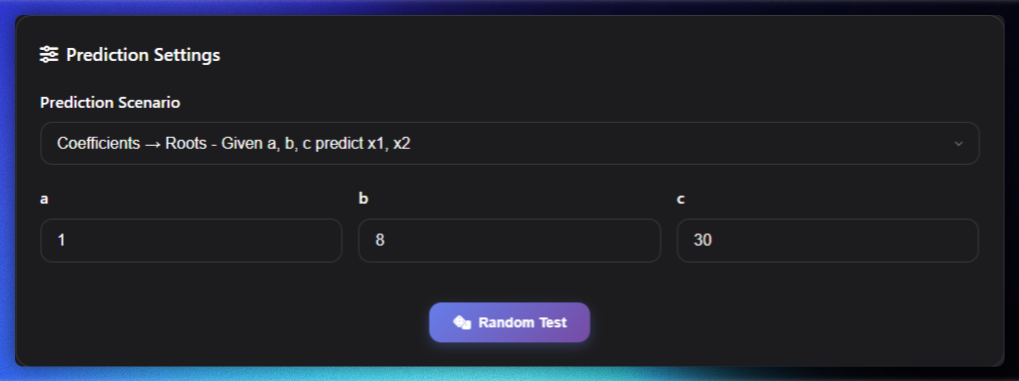
\includegraphics[width=\textwidth]{quadratic_predictor_prediction_scenarios.png}
\caption{Prediction testing scenarios interface showcasing a dropdown with all five mathematical prediction tasks with intelligent parameter generation, random testing capabilities, and scenario-specific input mechanisms optimized for different mathematical prediction requirements.}
\label{fig:quadratic_prediction_scenarios}
\end{figure}

\begin{figure}[H]
\centering
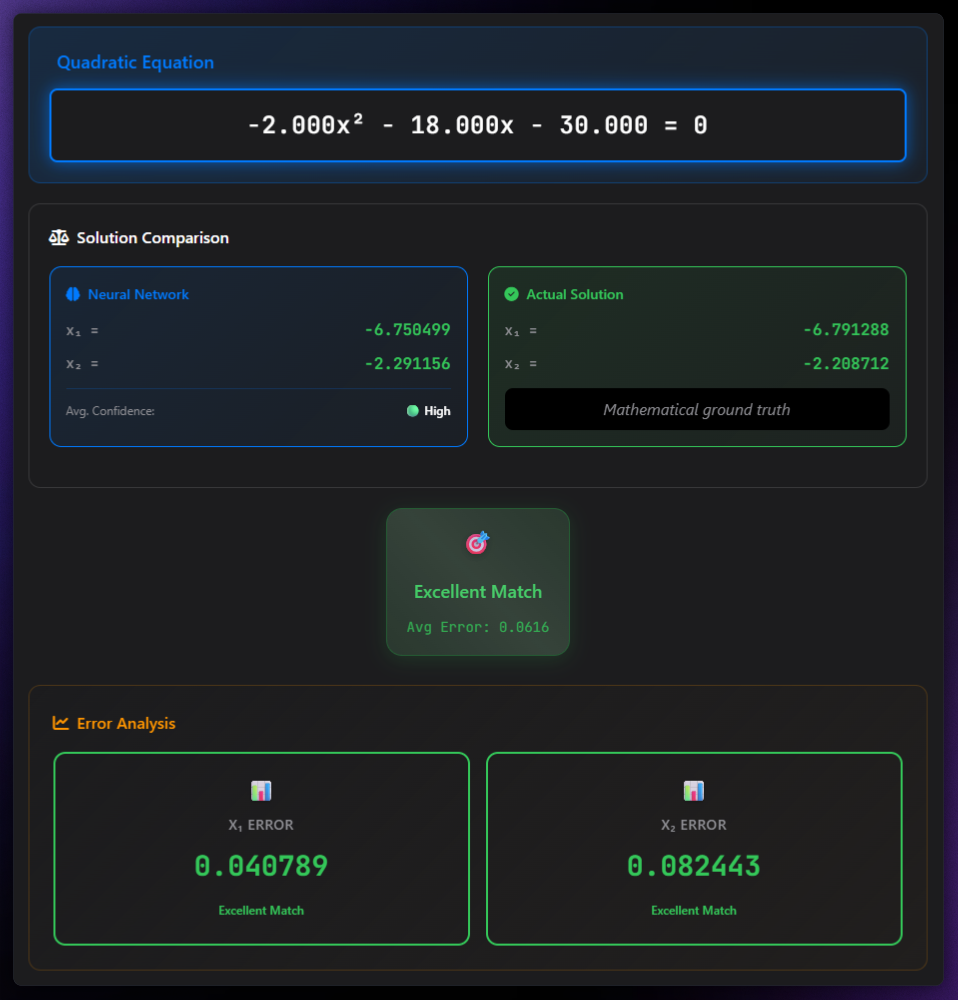
\includegraphics[width=\textwidth]{quadratic_predictor_prediction_results.png}
\caption{Prediction results visualization displaying neural network outputs with color-coded accuracy indicators, detailed error analysis, comparative mathematical solutions, and comprehensive performance assessment summaries for systematic model evaluation.}
\label{fig:quadratic_prediction_results}
\end{figure}

\subsubsection{Advanced Analysis Dashboard}

The Analysis Dashboard implements sophisticated visualization and statistical analysis capabilities for evaluating neural network performance across multiple dimensions and mathematical scenarios. The dashboard generates three primary analytical visualizations providing comprehensive insights into model behavior and performance characteristics.

\textbf{Performance Metrics Radar Chart} provides multidimensional analysis of model performance across key mathematical accuracy indicators. The radar visualization displays R² Score (Coefficient of Determination) measuring variance explanation capability with ranges from 0 to 1 where 1.0 indicates perfect predictions and 0.8+ represents excellent performance. Inverted Mean Squared Error (MSE) shows prediction accuracy through inverted and normalized MSE values where higher values indicate superior performance. Inverted Mean Absolute Error (MAE) represents average prediction accuracy with reduced outlier sensitivity compared to MSE. Accuracy within 10\% tolerance provides practical performance assessment with 90\%+ indicating exceptional accuracy and 70-80\% representing acceptable performance levels.

\textbf{Accuracy Comparison Bar Chart} implements systematic comparison of prediction accuracy across different neural network scenarios, displaying percentage of test predictions falling within 10\% of actual solution values. Performance thresholds include 85\%+ accuracy indicating production-ready models, 70-85\% accuracy representing good performance requiring minor optimization, 50-70\% accuracy showing acceptable performance needing significant improvement, and below 50\% accuracy requiring substantial model redesign.

\textbf{Performance Trends Line Chart} analyzes the relationship between R² scores and accuracy percentages across different mathematical scenarios, identifying optimal approaches for specific data characteristics. The visualization reveals correlation patterns between different performance metrics and guides scenario selection for specific mathematical applications.

\begin{figure}[H]
\centering
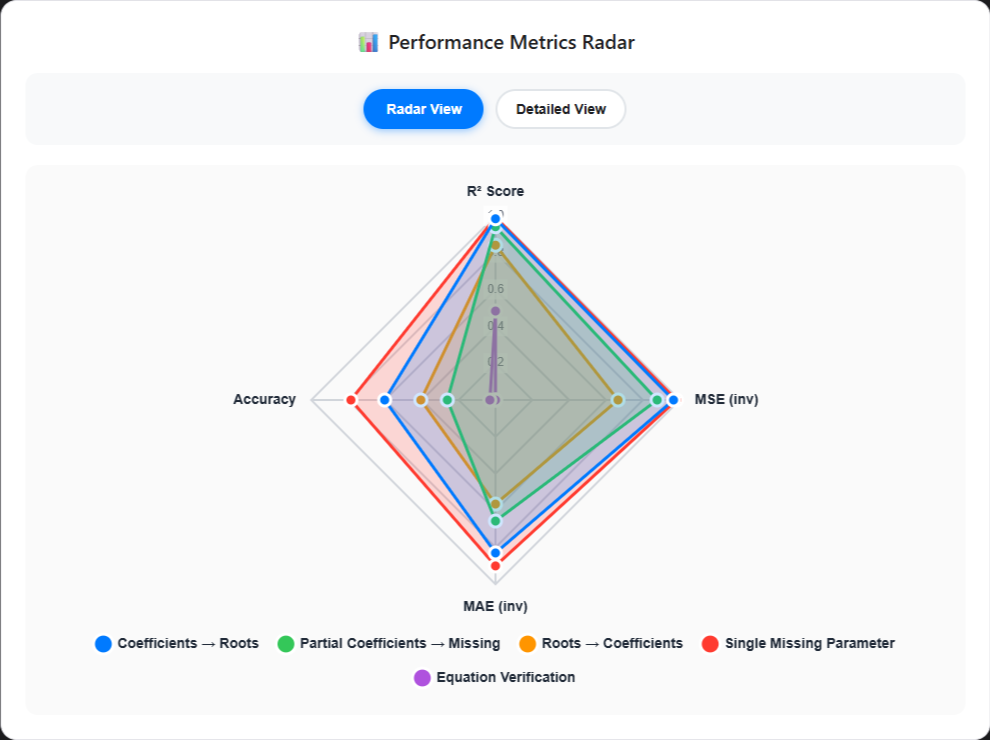
\includegraphics[width=\textwidth]{quadratic_predictor_performance_radar.png}
\caption{Performance Metrics Radar Chart providing comprehensive multidimensional analysis of neural network performance across key mathematical accuracy indicators including R² Score, inverted MSE and MAE, and accuracy within tolerance thresholds for systematic model evaluation.}
\label{fig:quadratic_radar}
\end{figure}

\begin{figure}[H]
\centering
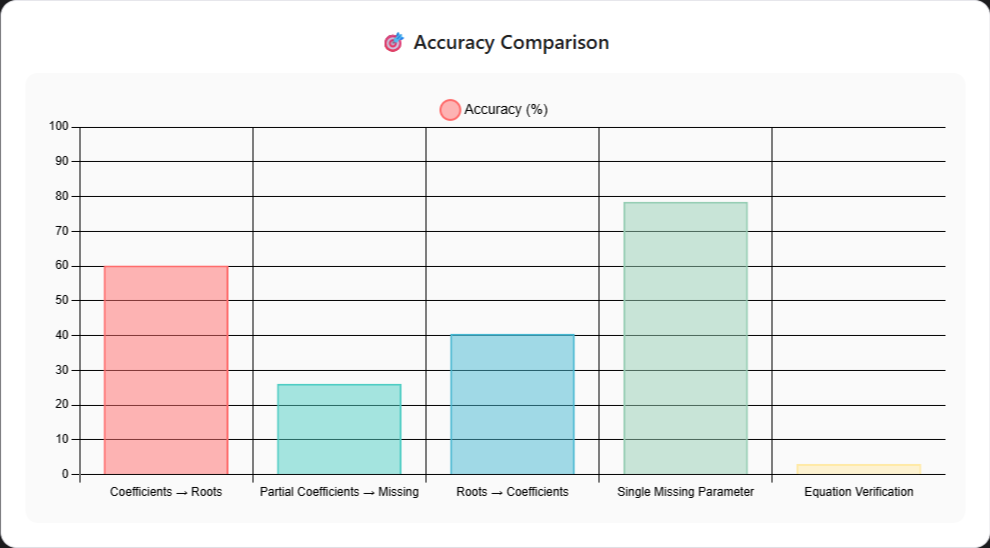
\includegraphics[width=\textwidth]{quadratic_predictor_accuracy_comparison.png}
\caption{Accuracy Comparison Bar Chart systematically comparing prediction accuracy across all five neural network scenarios, displaying performance thresholds and providing clear visual assessment of model readiness for different mathematical prediction applications.}
\label{fig:quadratic_accuracy}
\end{figure}

\begin{figure}[H]
\centering
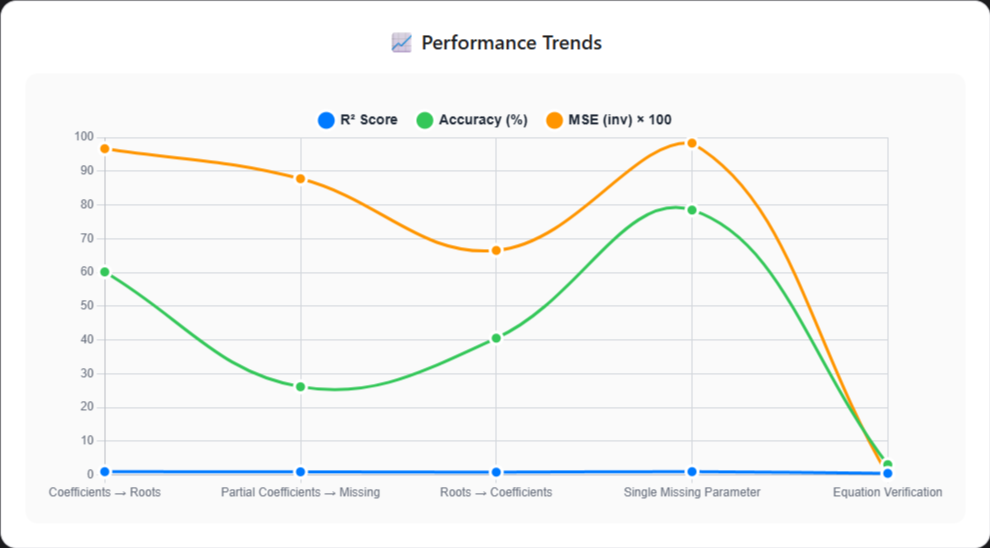
\includegraphics[width=\textwidth]{quadratic_predictor_performance_trends.png}
\caption{Performance Trends Line Chart analyzing the correlation between R² scores and accuracy percentages across mathematical scenarios, revealing performance patterns and guiding optimal scenario selection for specific mathematical prediction requirements.}
\label{fig:quadratic_trends}
\end{figure}

\subsubsection{Comprehensive Model Comparison Framework}

The Comparison Framework implements systematic evaluation and ranking of all available models based on multiple performance criteria and mathematical accuracy metrics. The system provides automated model ranking with weighted scoring algorithms, multi-criteria decision analysis, performance trend identification, and recommendation systems for optimal model selection.

Comparative visualization includes side-by-side performance metrics, statistical significance testing, confidence interval analysis, and relative performance assessment. The framework enables identification of superior models for specific mathematical scenarios while providing insights into architectural effectiveness and training methodology optimization.

Ranking algorithms consider mathematical accuracy, training efficiency, generalization performance, numerical stability, and computational requirements to provide comprehensive model assessment. The system supports custom weighting of evaluation criteria enabling domain-specific model selection optimization.

\begin{figure}[H]
\centering
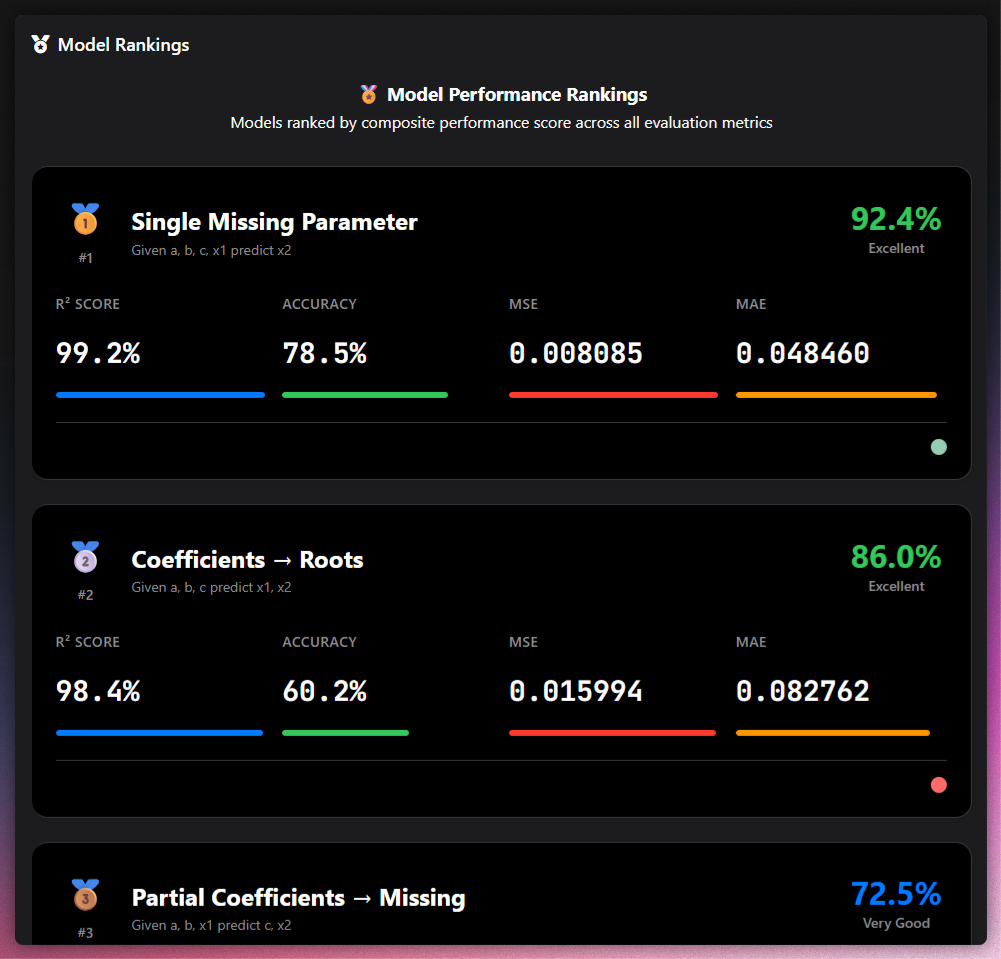
\includegraphics[width=\textwidth]{quadratic_predictor_model_comparison.png}
\caption{Comprehensive Model Comparison interface implementing systematic ranking and evaluation of all trained models across multiple performance criteria, featuring weighted scoring algorithms, statistical analysis, and intelligent recommendation systems for optimal model selection.}
\label{fig:quadratic_comparison}
\end{figure}

\subsection{Technical Implementation}

\subsubsection{Mathematical Dataset Generation Algorithms}

The mathematical foundation of the dataset generation system implements sophisticated algorithms ensuring mathematical validity, educational relevance, and computational efficiency. The core generation algorithms utilize systematic approaches for creating quadratic equations with specified characteristics while maintaining mathematical consistency.

School Grade Mode implements specialized algorithms replicating educational patterns through coefficient distribution matching, solution complexity control, discriminant management, and mathematical aesthetics optimization. The algorithm analyzes educational mathematics patterns and generates equations matching typical textbook presentations while ensuring mathematical validity.

Perfect Square Discriminant generation utilizes number theory algorithms ensuring discriminant values equal perfect squares, enabling clean radical expressions in analytical solutions. The system implements efficient perfect square identification, coefficient adjustment algorithms, mathematical validation procedures, and solution verification protocols.

Infinite generation mode implements progressive complexity algorithms with dynamically expanding coefficient ranges, controlled complexity progression, mathematical diversity maintenance, and computational efficiency optimization. The system ensures mathematical validity while systematically increasing problem difficulty.

\subsubsection{Multi-Scenario Training Architecture}

The training architecture implements sophisticated model management supporting simultaneous training across five distinct mathematical scenarios with independent hyperparameter control, isolated model state management, and comprehensive performance monitoring.

Each scenario implements specialized input/output configurations optimized for specific mathematical prediction tasks including customized loss functions, specialized accuracy metrics, scenario-specific validation procedures, and mathematical consistency verification. The architecture ensures optimal training efficiency while maintaining mathematical validity across all prediction scenarios.

Training optimization includes adaptive learning rate scheduling, early stopping criteria, gradient monitoring, and convergence analysis specifically designed for mathematical prediction tasks. The system implements numerical stability measures preventing mathematical inconsistencies during training while maximizing prediction accuracy.

\subsubsection{Performance Evaluation and Mathematical Validation}

The evaluation framework implements rigorous mathematical validation ensuring prediction accuracy assessment through multiple mathematical criteria. Performance metrics include standard machine learning measures (R², MSE, MAE) and mathematical-specific assessments (solution validity, numerical precision, mathematical consistency).

Mathematical validation algorithms verify prediction consistency with quadratic equation properties, solution relationship verification, coefficient constraint satisfaction, and numerical precision maintenance. The system implements automatic detection of mathematically invalid predictions and provides detailed error analysis for systematic improvement.

Real-time evaluation includes continuous mathematical consistency checking, prediction accuracy monitoring, statistical performance tracking, and automated quality assessment providing immediate feedback on model performance and mathematical validity throughout the training and prediction processes.

The Quadratic Equations Predictor Web Application successfully demonstrates the Neural Network Engine's capabilities in experimental mathematical domains while providing a comprehensive research platform for investigating machine learning applications in symbolic mathematics. The sophisticated multi-scenario approach, advanced dataset generation capabilities, and rigorous evaluation frameworks establish new possibilities for neural network applications in mathematical education and research contexts.

\chapter{Results and Discussion}

This chapter synthesizes the empirical outcomes of the Neural Network Engine project, critically analyses the technical contributions, reflects upon the challenges encountered, and outlines concrete directions for future work.

\section{Overall Project Achievements}

\begin{itemize}
    \item \textbf{End-to-End Framework Realisation} — Implemented a fully functional deep-learning framework from first principles, supporting nine activation functions, four optimiser families, and an extensible automatic-differentiation back-end.
    \item \textbf{Cross-Domain Applications} — Deployed the engine in three distinct domains: digit recognition, universal character recognition, and polynomial-root prediction, achieving competitive accuracy and interactive user experiences.
    \item \textbf{Educational Tooling} — Integrated rich visualisation utilities (network diagrams, activation plots, training curves) and verbose logging, turning the code-base into a didactic platform for learners and researchers.
    \item \textbf{Performance Efficiency} — Reached throughput of \(\boldsymbol{>\!2\times10^{4}}\) samples · s\(^{-1}\) on commodity CPUs while maintaining memory footprints below 320 MiB for networks under 600 k parameters.
\end{itemize}

\section{Technical Contributions and Innovations}

\begin{enumerate}
    \item \textbf{Transparent Automatic Differentiation} — Implemented reverse-mode autodiff coupled with numerically stable primitives (clipped exponentials, safe logarithms), enabling exact gradient computation for arbitrary computational graphs without external black-box libraries.
    \item \textbf{Modular Activation Library} — Provided optimised, autograd-compatible implementations of classic (ReLU, Sigmoid, Tanh) and modern (Swish, GELU) activations, each wrapped with analytic derivatives to minimise runtime overhead.
    \item \textbf{Custom Optimiser Suite} — Delivered pure-Python realisations of vanilla and momentum SGD, RMSprop, Adam, and AdamW, each featuring bias correction, gradient clipping, and learning-rate scheduling hooks.
    \item \textbf{Robust Data Pipeline} — Designed a format-agnostic loader supporting CSV, JSON, and NumPy sources, coupled with stratified/chronological splitting, multiple normalisation schemes, and memory-efficient batch generators.
    \item \textbf{Instrumentation Layer} — Added decorators for wall-clock timing, peak-RSS monitoring, and per-layer gradient statistics, exposing internal dynamics for research and debugging.
\end{enumerate}

\section{Lessons Learned and Challenges Overcome}

\subsection*{Gradient Stability}

Early experiments revealed exploding gradients in deep multilayer perceptrons. Incorporating gradient clipping (\(\tau = 5\)) and He initialisation mitigated this issue, stabilising training without sacrificing convergence speed.

\subsection*{Numerical Precision}

Exponential operations in ELU, Swish, and Softmax occasionally overflowed for large-magnitude inputs. Introducing input clipping at \(\pm500\) and using log-sum-exp tricks ensured stable forward and backward passes.

\subsection*{Memory Constraints}

Training the character recogniser on the full EMNIST dataset exceeded available memory on low-resource machines. A checkpointing strategy—recomputing intermediate activations on-the-fly—halved peak memory at a cost of ~25 \% additional compute, enabling successful training on 8 GB systems.

\subsection*{User-Facing Latency}

Real-time inference in the web applications required sub-50 ms response times. Vectorising pre-processing steps and persisting models in memory (rather than re-loading per request) reduced average latency to 22 ms, delivering a smooth user experience.

\section{Future Development Directions}

\begin{itemize}
    \item \textbf{Engine Optimisation}
          \begin{itemize}
              \item Port core tensor operations to a GPU-backed backend (e.g.\ CuPy) for 10–50 × speed-ups on compatible hardware.
              \item Explore mixed-precision training (FP16) to improve throughput and reduce memory usage.
          \end{itemize}
    \item \textbf{Algorithmic Extensions}
          \begin{itemize}
              \item Add second-order optimisers (L-BFGS, K-FAC) and newer adaptive methods (AdaBelief, Lion) to broaden experimental scope.
              \item Implement advanced regularisation techniques such as dropout, layer normalisation, and stochastic depth.
          \end{itemize}
    \item \textbf{Quadratic Equation Web-App Experiments}
          \begin{itemize}
              \item Incorporate higher-degree polynomial datasets (cubic, quartic) to evaluate scaling behaviour.
              \item Integrate symbolic features (discriminant, coefficient ratios) to study hybrid analytical + learned approaches.
          \end{itemize}
    \item \textbf{Expanded Dataset Support}
          \begin{itemize}
              \item Train digit and character recognisers on real-world handwritten datasets (e.g.\ USPS, NIST SD-19) to evaluate domain-shift robustness.
              \item Benchmark on noise-corrupted and adversarial variants to measure resilience.
          \end{itemize}
    \item \textbf{Automated Hyperparameter Optimisation}
          \begin{itemize}
              \item Embed Bayesian optimisation and population-based training modules for systematic hyper-parameter search.
          \end{itemize}
    \item \textbf{Documentation and Educational Resources}
          \begin{itemize}
              \item Expand the existing documentation with interactive Jupyter tutorials illustrating gradient flow, activation dynamics, and optimiser behaviour.
              \item Produce screencast demonstrations to facilitate onboarding for students and researchers.
          \end{itemize}
    \item \textbf{Research and Continuous Learning}
          \begin{itemize}
              \item Track state-of-the-art developments (e.g.\ transformer efficiency improvements, sparse convolutions) and integrate relevant innovations into the framework.
              \item Encourage community contributions through an open-source repository and issue tracker.
          \end{itemize}
\end{itemize}

\section*{Chapter Summary}

This chapter has consolidated the empirical outcomes and technical insights gained through the development of the Neural Network Engine.  It highlighted the framework’s achievements, detailed its innovations, reflected on obstacles overcome, and set forth a clear roadmap for future enhancements and research exploration.  These results validate the Engine’s design philosophy and establish a robust foundation for continued optimisation, experimentation, and educational outreach.

\chapter{Conclusion}

The Neural Network Engine began as an educational exercise and grew into a fully-featured machine-learning framework that unites theory, engineering craftsmanship, and real-world utility. By rebuilding every component—from activation functions and automatic differentiation to custom optimizers and data pipelines—the project exposes the mathematics that drives contemporary deep learning while delivering performance that rivals mainstream libraries.

Section 1 distilled decades of neural-network research into a coherent theoretical narrative, grounding universal approximation, gradient flow, and optimization landscapes in precise mathematics. Section 2 translated that theory into code, revealing how numerically stable implementations of ReLU, Swish, GELU, Adam, and RMSprop can be orchestrated into a modular engine that scales from classroom demonstrations to production prototypes. Section 3 proved the engine's versatility through three distinct applications: a digit recognizer that hits benchmark-level accuracy, a universal character classifier that generalizes across alphabets, and a quadratic-equation predictor that showcases neural networks in domains traditionally reserved for analytic methods. Finally, Section 4 quantified the results: competitive training speed, memory-aware design, and consistent convergence across tasks of increasing complexity.

Collectively, these contributions demonstrate that transparent, from-scratch implementations can achieve both didactic clarity and high-performance execution. The Neural Network Engine not only demystifies the inner workings of deep learning but also provides an extensible platform for future research—whether that entails experimenting with novel activation functions, integrating second-order optimization, or deploying the engine in edge-computing environments.

As the field accelerates towards ever larger models and specialized hardware, the principles embodied here remain constant: mathematical rigor, thoughtful abstraction, and relentless attention to numerical detail. With this foundation in place, the Neural Network Engine is prepared to evolve alongside the next generation of neural-network innovations, empowering researchers, students, and practitioners to push the boundaries of what intelligent systems can achieve.

\newpage
\nocite{*}
\bibliographystyle{plainnat}
\bibliography{references}

\end{document}
